%\documentclass[a4paper,12pt,twoside]{book}
\documentclass[listof=nochaptergap,12pt,times]{report}
\usepackage{mathptmx}%This package supersedes times and mathptm
\usepackage[a4paper,right=2.54cm,left=2.54cm,top=2.54cm,bottom=2.54cm]{geometry}
\usepackage{array}
\usepackage{listings}
\usepackage{pdflscape}
\usepackage{longtable}
\usepackage{enumitem}
\newcolumntype{C}[1]{>{\centering\arraybackslash}p{#1}}
\newcolumntype{N}{@{}m{0pt}@{}}

%%Paquete para ocultar indices de tabla de contenidos
%% Numeración continua en figuras y tablas
\setcounter{equation}{0}
\usepackage{chngcntr}
\counterwithout{figure}{chapter}
\counterwithout{table}{chapter}
\counterwithout{equation}{chapter}
\renewcommand{\thefigure}{\arabic{figure}}
\renewcommand{\thetable}{\arabic{table}}
\renewcommand{\theequation}{\arabic{equation}}

% Parche para eliminar espacios por capítulos en lista de figuras y tablas
\usepackage{etoolbox}% http://ctan.org/pkg/etoolbox
\makeatletter
% \patchcmd{<cmd>}{<search>}{<replace>}{<succes>}{<failure>}
\patchcmd{\@chapter}{\addtocontents{lof}{\protect\addvspace{10\p@}}}{}{}{}% LoF
\patchcmd{\@chapter}{\addtocontents{lot}{\protect\addvspace{10\p@}}}{}{}{}% LoT
\makeatother

%%%%paquete para usar citas de diferentes formatos
%%%%%%%%%%%%%%%%%%%%%%%%%%%%%%%%%
%%add al indice
%\usepackage[nottoc,numbib]{tocbibind}
%\usepackage[authoryear,round]{natbib}
\usepackage[utf8]{inputenc}
\usepackage{csquotes}
\usepackage[spanish,es-lcroman]{babel}
\decimalpoint
%% Citas y bibliografía formato APA
\usepackage[style=apa ,
%hyperref=auto,
%citestyle=authoryear,
natbib=true,
backend=biber]{biblatex}
\addbibresource{biblio/references.bib}
%% Convertir comando cita por textcite para que tenga formato APA
\let\cite\textcite

%% Para que texto de figuras y tablas tenga formato APA
\usepackage{multirow,booktabs,setspace,caption}
\DeclareCaptionLabelSeparator*{spaced}{\\[2ex]}
\captionsetup[table]{textfont=it,format=plain,justification=justified,
	singlelinecheck=false,labelsep=spaced,skip=0pt}
\captionsetup[figure]{labelsep=period,labelfont={it,bf},justification=justified,singlelinecheck=false,font=doublespacing}
\captionsetup[subfigure]{justification=centering}

%%%Editar formato y tamaño de capítulos y secciones
\usepackage{titlesec}
\titleformat{\chapter}
{\normalfont\large\bfseries}{CAPÍTULO \thechapter:}{1em}{}
\titlespacing*{\chapter}{0pt}{-4ex}{1ex}

\titleformat{\section}
{\normalfont\large\bfseries}{\thesection}{1em}{}
\titlespacing*{\section}{0pt}{0pt}{0pt}

\titleformat{\subsection}
{\normalfont\large\bfseries}{\thesubsection}{1em}{}
\titlespacing*{\subsection}{0pt}{0pt}{0pt}

%\usepackage{biblatex}
%paquete para hiperlinks entre citas e imagenes
%%%%%%%%%%%%%%%%%%%%%%%%%%%%%%%%%
\usepackage[colorlinks=true,
citecolor=black,
urlcolor=black,
bookmarks=true,
linkcolor=black,
pdftitle={Tesis-nombre-alumno},
pdfauthor={autor nombres}]{hyperref}

\usepackage{amssymb}
\usepackage{graphicx} % for improved inclusion of graphics
%\usepackage{wrapfig} % to include figure with text wrapping around it
\usepackage[margin=10pt,font=small,labelfont=bf]{caption} % for improved layout of figure captions with extra margin, smaller font than text
\usepackage{subcaption}
\usepackage{eucal}
\usepackage[usenames, dvipsnames]{color}
\usepackage[perpage]{footmisc}
%\usepackage[round, sort]{natbib}
\usepackage{ifthen}
\usepackage{multicol} % for pages with multiple text columns, e.g. References
\setlength{\columnsep}{20pt} % space between columns; default 10pt quite narrow
%% Para no mostrar índices de figuras ni tablas en el índice general
\usepackage[nottoc,notlot,notlof]{tocbibind}
%\usepackage{appendix}
\usepackage[titletoc,title]{appendix} 

%%%----Modificar encabezado y pie de pagina
%%%%%%%%%%%%%%%%%%%%%%%%%%%%%%%%%%%%%%%%%%%%%%%%%%%%%%%%%%%%%%%%%%%%%
\usepackage{fancyhdr} % for better header layout
\newcommand{\changefont}{%
	\fontsize{9pt}{1.5pt}\selectfont
}

\pagestyle{fancy}
%%Para borrar fancy por default (incluye numeracion)
\fancyhf{} % sets both header and footer to nothing
%%Para borrar linea de encabezado
\renewcommand{\headrulewidth}{0pt}
%%Encabezados solo con numero de pagina
\fancypagestyle{normal}{%
	\fancyhead{} % clear all header fields
	\fancyhead[R]{\thepage}}
%%Encabezados con titulo de tesis y numero de pagina
\fancypagestyle{special}{%
	\fancyhead[L]{\changefont Predicción del estado de financiamiento de proyectos de tecnología en sitio web de crowdfunding Kickstarter mediante modelo de Aprendizaje Profundo Multimodal}
	\fancyhead[R]{\thepage}}


%\fancyhf{} %% delete default configuration of page
%%\setlength\headheight{15pt}

%%%%%%%%%%%%%%%%%%%%%%%%%%%%%5
%%%% Configuracion de los parrafos
%\usepackage{setspace}
%\onehalfspacing
%\linespread{1.25} 
\setlength{\parindent}{0.5in} %%sangria
\setlength{\parskip}{3mm}  %%espacio entre parrafos
\linespread{1.3} %This equals 1.5 linespacing in Word
%%%% nuevo parrafo
%%%%%%%%%%%%%%%%%%%%%%%%%%%%%5
%%%% Centrar valores de una tabla
\usepackage{array}
%%CENTRADO HORIZONTAL
\newcolumntype{P}[1]{>{\centering\arraybackslash}p{#1}}
%%CENTRADO VERTICAL
\newcolumntype{M}[1]{>{\centering\arraybackslash}m{#1}}

%%%%%%%%%%%%%%%%%%%%%%%%%%%%%5
%%%%Paquete para alinear texto
\usepackage{ragged2e}
\usepackage{multirow}
\usepackage{makecell}
\usepackage{rotating}
\usepackage{siunitx} % To align the numbers later on
\usepackage[table,xcdraw]{xcolor}
\usepackage{color, colortbl}
\definecolor{Gray}{gray}{0.9}
\definecolor{orange}{rgb}{1,0.647,0}
\definecolor{turq3}{rgb}{0.54, 0.81, 0.94}
\definecolor{turq}{rgb}{0.63, 0.79, 0.95}
\definecolor{bluejean}{rgb}{0.03, 0.27, 0.49}

%%%%%%%%%%%%%%%%%%%%%%%%%
\usepackage{xparse}
\usepackage{expl3}
%%%%funcion de reemplazar regex
\ExplSyntaxOn
\NewDocumentCommand{\replace}{mmm}
{
	\marian_replace:nnn {#1} {#2} {#3}
}

\tl_new:N \l_marian_input_text_tl
\tl_new:N \l_marian_search_tl
\tl_new:N \l_marian_replace_tl

\cs_new_protected:Npn \marian_replace:nnn #1 #2 #3
{
	\tl_set:Nn \l_marian_input_text_tl { #1 }
	\tl_set:Nn \l_marian_search_tl { #2 }
	\tl_set:Nn \l_marian_replace_tl { #3 }
	\regex_replace_all:nnN { \b\u{l_marian_search_tl}\b } { \u{l_marian_replace_tl} } \l_marian_input_text_tl
	\tl_use:N \l_marian_input_text_tl
}
\ExplSyntaxOff

%%%%%%%%%%%%%%%%%%%%%%%%%%%%%%%%%%%%%%
\usepackage{amsmath}
%\setcounter{equation}{0}
%\numberwithin{equation}{chapter} %%enumerar ecuaciones
%\renewcommand{\theequation}{Ecuación \arabic{equation}}   
\usepackage{mathtools, nccmath, cool}
%%%Configuraciones de biblatex

%%%hel
%%%%\citeauthor
\makeatletter

%%%%%%%%%%%%
\DeclareCiteCommand{\citeauthor}
{\boolfalse{citetracker}%
	\boolfalse{pagetracker}%
	\usebibmacro{prenote}}
{\ifciteindex
	{\indexnames{labelname}}
	{}%
	\printtext[bibhyperref]{\printnames{labelname}}}
{\multicitedelim}
{\usebibmacro{postnote}}


\DeclareCiteCommand{\citetitle}
{\boolfalse{citetracker}%
	\boolfalse{pagetracker}%
	\usebibmacro{prenote}}
{\ifciteindex
	{\indexfield{indextitle}}
	{}%
	\printtext[bibhyperref]{\printfield[citetitle]{labeltitle}}}
{\multicitedelim}
{\usebibmacro{postnote}}

\DeclareCiteCommand{\cite}
{\usebibmacro{prenote}}
{\usebibmacro{citeindex}%
	\printtext[bibhyperref]{\usebibmacro{cite}}}
{\multicitedelim}
{\usebibmacro{postnote}}

\DeclareCiteCommand*{\cite}
{\usebibmacro{prenote}}
{\usebibmacro{citeindex}%
	\printtext[bibhyperref]{\usebibmacro{citeyear}}}
{\multicitedelim}
{\usebibmacro{postnote}}

\DeclareCiteCommand{\parencite}[\mkbibparens]
{\usebibmacro{prenote}}
{\usebibmacro{citeindex}%
	\printtext[bibhyperref]{\usebibmacro{cite}}}
{\multicitedelim}
{\usebibmacro{postnote}}

\DeclareCiteCommand*{\parencite}[\mkbibparens]
{\usebibmacro{prenote}}
{\usebibmacro{citeindex}%
	\printtext[bibhyperref]{\usebibmacro{citeyear}}}
{\multicitedelim}
{\usebibmacro{postnote}}

\DeclareCiteCommand{\footcite}[\mkbibfootnote]
{\usebibmacro{prenote}}
{\usebibmacro{citeindex}%
	\printtext[bibhyperref]{ \usebibmacro{cite}}}
{\multicitedelim}
{\usebibmacro{postnote}}

\DeclareCiteCommand{\footcitetext}[\mkbibfootnotetext]
{\usebibmacro{prenote}}
{\usebibmacro{citeindex}%
	\printtext[bibhyperref]{\usebibmacro{cite}}}
{\multicitedelim}
{\usebibmacro{postnote}}

\DeclareCiteCommand{\textcite}
{\boolfalse{cbx:parens}}
{\usebibmacro{citeindex}%
	\printtext[bibhyperref]{\usebibmacro{textcite}}}
{\ifbool{cbx:parens}
	{\bibcloseparen\global\boolfalse{cbx:parens}}
	{}%
	\multicitedelim}
{\usebibmacro{textcite:postnote}}
\makeatother
\makeatletter
\let\abx@macro@citeOrig\abx@macro@cite
\renewbibmacro{cite}{%
	\bibhyperref{%
		\let\bibhyperref\relax\relax%
		\abx@macro@citeOrig%
	}%
}
\let\abx@macro@textciteOrig\abx@macro@textcite
\renewbibmacro{textcite}{%
	\bibhyperref{%
		\let\bibhyperref\relax\relax%
		\abx@macro@textciteOrig%
	}%
}%

\makeatother

%%%%%%%%%%%%%%%%%%%%%%%%%%%%%%%%%%%%%%%%%%%
% Agregando librerias para que aparezca texto debajo de las ecuaciones.
\usepackage{tocloft}
\usepackage{xpatch}
\usepackage{caption}
\DeclareCaptionType{equcaption}[Ecuación][Índice de Ecuaciones]

\newenvironment{conditions}
{\par\vspace{\abovedisplayskip}\noindent\begin{tabular}{>{$}l<{$} @{${}={}$} l}}
	{\end{tabular}\par\vspace{\belowdisplayskip}}

%\usepackage[titles]{tocloft}

% Para agregar linea de puntos en la tabla de contenidos
\renewcommand{\cftpartleader}{\cftdotfill{\cftdotsep}} % for parts
\renewcommand{\cftchapleader}{\cftdotfill{\cftdotsep}} % for chapters

% Para eliminar linea de puntos de la tabla de contenidos
%\renewcommand{\cftdot}{}

% Para alinear párrafo en indice de figuras y tablas
\cftsetindents{figure}{0em}{2.5em}
\renewcommand\cftfigpresnum{\figurename~}
\renewcommand{\cftfigaftersnum}{.} % Goes after figure number
\newlength\mylength
\settowidth\mylength{\cftfigpresnum}
\addtolength\cftfignumwidth{\mylength}
\cftsetindents{table}{0em}{2.5em}
\renewcommand\cfttabpresnum{Tabla }
\renewcommand{\cfttabaftersnum}{.} % Goes after figure number
\settowidth\mylength{\cfttabpresnum}
\addtolength\cfttabnumwidth{\mylength}

\begin{document}
% Se añade esto para agregar la lista de ecuaciones en el indice del documento	

\newcommand{\listequationsname}{Índice de Ecuaciones}
\newlistof{myequations}{equ}{\listequationsname}
\newcommand{\myequations}[1]{%
	\addcontentsline{equ}{myequations}{Ecuación \protect\numberline{\theequation}#1}\par}
%\addcontentsline{toc}{section}{Índice de Ecuaciones}

%%Numeros de pagina en romano (minuscula)
%\pagenumbering{roman}
\renewcommand{\thepage}{\roman{page}}

% Beginning of hack...
%\let\oldthispagestyle=\thispagestyle % If we want to see a page number.
%\def\thispagestyle#1{} % If we want to see a page number.
%\let\oldsetcounter=\setcounter
%\def\setcounter#1#2{}
% End of hack...

\begin{titlepage}

	\begin{center}
		%%%cargar imagen
	    
\includegraphics[width=0.45\textwidth]{images_repo/esanlogomin}
		\vspace*{2cm} \\
		UNIVERSIDAD ESAN \vspace*{1ex} \\
		FACULTAD DE INGENIERÍA \vspace*{1ex} \\
		INGENIERÍA DE TECNOLOGÍAS DE INFORMACIÓN Y SISTEMAS
		\vspace*{8ex} \\
		%\textbf
		{Predicción del estado de financiamiento de proyectos de tecnología en sitio web de crowdfunding Kickstarter mediante modelo de Aprendizaje Profundo Multimodal}
		\vspace*{8ex}\\	
		Tesis para optar el Título de Ingeniero de Tecnologías de Información y Sistemas que presenta: 
		\vspace*{8ex} \\	
		Alonso Augusto Puente Ríos \\
		Asesor: Marks Arturo Calderón Niquin		
		\vfill
		
		Lima, \today 
		
	\end{center}
\end{titlepage}
%%Permite mostrar encabezado y numeracion en primera pagina de capitulos - indices
\fancypagestyle{plain}{}
%%cambiar nombres de objetos para el indice y otros
\renewcommand{\listfigurename}{Índice de Figuras}
\renewcommand{\tablename}{Tabla}
\renewcommand{\listtablename}{Índice de Tablas}
%%Permite empezar conteo de paginas de forma personalizada
\addtocounter{page}{1}
\pagestyle{normal}
%\thispagestyle{plain}
%\vspace{0.5cm}
\leftline{Esta tesis denominada:}
\begin{center}
	%\vspace*{10cm}
	{PREDICCIÓN DEL ESTADO DE FINANCIAMIENTO DE PROYECTOS DE TECNOLOGÍA EN WEB DE CROWDFUNDING KICKSTARTER MEDIANTE MODELO DE APRENDIZAJE PROFUNDO}
\end{center}

\leftline{ha sido aprobada.}
\vspace{2.5cm}

\dotfill

\rightline{(Jurado Presidente)}
\vspace{1.5cm}

\dotfill

\rightline{(Jurado)}
\vspace{1.5cm}

\dotfill

\rightline{(Jurado)}
\vspace{1.5cm}

\centerline{Universidad ESAN}
\centerline{2021}
%\thispagestyle{plain}
\begin{center}
	\vspace*{10cm}
	{PREDICCIÓN DEL ESTADO DE FINANCIAMIENTO DE PROYECTOS DE TECNOLOGÍA EN WEB DE CROWDFUNDING KICKSTARTER MEDIANTE MODELO DE APRENDIZAJE PROFUNDO}
\end{center}

%\thispagestyle{plain}
\begin{center}
	%\vspace*{1.5cm}
	{\Large \bfseries  Agradecimiento y Dedicatoria}
\end{center}
\vspace{0.5cm}

Durante la inducción en la empresa en la cual realicé mis segundas prácticas pre-profesionales, se realizaron varias actividades, entre ellas, una que me marcó positivamente. Esta consistía en comparar los tiempos de llegada de un punto a otro de una persona corriendo. Se caracterizó porque quien asumió el reto tuvo presente en su mente las personas y las razones por las cuales todos los días lucha y son su principal fuente de motivación.

Por ello, quiero dedicar este gran esfuerzo personal de trabajo de tesis a quienes siempre han estado a mi lado en los mejores y peores momentos, aquellos críticos en que definen el destino. Mi amada hermana Clarisabel, mis queridos padres Augusto e Isabel, mi familia en especial mis abuelos; y mis pocos, pero verdaderos y leales amigos de la universidad, colegio y trabajo. Todos ellos han sido y son cada uno, piedra fundamental en el desarrollo de mi ser como persona y profesional, así como también seres con los cuales siempre comparto gratos momentos. Su presencia en mi vida no ha sido una suerte más sino parte de mi destino.
Asimismo, luchar por mis sueños y mi país, y pensar cada día en solidificar su planificación me motivan emocionalmente hasta en aquellos momentos en que parece haber imposibles.

Quiero concluir esta sección, muy especial para mí, agradeciendo también a mi alma máter, la Universidad Esan, y al Programa Nacional de Becas (Pronabec) por hacer que estos 5 años entre el 2015 y 2019 sean mágicos y muy fructíferos. Tuve la oportunidad no solo de incrementar y potenciar mis conocimientos en distintas áreas académicas sino también de aprender de excelentes profesionales como mis profesores, conocer grandes amigos dentro y fuera de su campus (desde el primer ciclo como cachimbo hasta el último ciclo, en el CADE Universitario 2019, estudiantes de diferentes universidades y otras partes del Perú), ponerme a prueba en el exterior (en el II Congreso Internacional de Investigación en Colombia en el año 2017, y en el Summer School of Machine Learning en Rusia en el año 2020 luego de obtener mi grado de bachiller) y formar parte de la gran familia UE.

Por todos ellos, simplemente gracias.
\newline



% outline
\tableofcontents            % print the table of contents

%: ----------------------- contents ------------------------

\setcounter{secnumdepth}{3} % organisational level that receives a numbers
\setcounter{tocdepth}{3}    % print table of contents for level 3

% levels are: 0 - chapter, 1 - section, 2 - subsection, 3 - subsection


%: ----------------------- list of figures/tables ------------------------
\clearpage
\listoffigures
\clearpage
\listoftables  % print list of tables
\clearpage
\phantomsection
%\listofequcaptions % print list of equations
\listofmyequations
\clearpage
%%Numeros de pagina en arabic
\renewcommand{\thepage}{\arabic{page}}
%%Encabezado con titulo de tesis y numeracion
\pagestyle{special}
\thispagestyle{plain}
\begin{center}
	%\vspace*{1.5cm}
	{\Large \bfseries  Resumen}
\end{center}
\vspace{0.5cm}

Conocer el destino del financiamiento de proyectos siempre ha sido el principal deseo de todos los emprendedores que los promocionan en Internet, en especial, de la categoría de tecnología por ser los que presentan las ratios más bajas de éxito debido a sus altas metas que buscan alcanzar. El presente trabajo de investigación se basó en construir un modelo predictivo cuyo objetivo es la de estimar el éxito o fracaso de financiamiento de proyectos tecnológicos en la plataforma de crowdfunding Kickstarter durante su campaña a partir de su metainformación, descripción y comentarios de los patrocinadores. Para ello, se creó un Modelo Apilado Integrado de modelos de Aprendizaje Profundo para cada modalidad, denominada The Hydra. Luego de analizar los resultados del modelo final con las métricas mencionadas en la literatura, se concluyó que el modelo propuesto presentó mejor rendimiento que la mayoría de los antecedentes debido a la mejora de su capacidad colectiva por encima de cada performance individual que lo compone. Como trabajo a futuro, el sistema piloto que incluye al modelo será insertada en una plataforma web, se afinarán más hiperparámetros y se considerarán más variables potenciales.
%\newline

\textbf{Palabras claves: } metainformación, descripción, comentarios, Aprendizaje Profundo, Modelo Apilado, Perceptrón Multicapa (MLP), Red Neuronal Convolucional (CNN), Red Neuronal Recurrente (RNN).

\vspace{0.5cm}
Knowing funding projects destiny has always been the main desire of all entrepreneurs who promote them on the Internet, especially in the technology category because they have the lowest success rates due to their high goals. The present research work was based on building a predictive model whose objective is to estimate the success or failure of technological projects funding in the Kickstarter crowdfunding platform during its campaign based on its metadata, description and backers comments. For this, an Integrated Stacking Model based on Deep Learning models for each modal created, called The Hydra. After analyzing the final model results with metrics mentioned in the literature, it was concluded that the proposed model presented better performance than most of the antecedents due to the improvement of its collective capacity over each individual performance that composes it. As work in the future, the pilot system that includes the model will be inserted into a web platform, more hyperparameters will be refined and more potential variables will be considered.
%\newline

\textbf{Keywords: } project metadata, project description, project comments, Deep Learning, Stacked Model, Multilayer Perceptron (MLP), Convolutional Neural Network (CNN), Recurrent Neural Network (RNN).
%La línea de abajo es para quitar encabezado
%\thispagestyle{plain}

\chapter*{INTRODUCCIÓN}
\markboth{INTRODUCCIÓN}{INTRODUCCIÓN}
\addcontentsline{toc}{chapter}{INTRODUCCIÓN}

Por muchos años, en especial en las dos últimas décadas, diversos proyectos emprendedores han sido lanzados en distintas plataformas web, buscando un objetivo compartido por todos: ser financiados en un determinado plazo para hacer realidad estas ideas. Entre fracasos y éxitos, han surgido nuevas tendencias, así como nuevas perspectivas de estudios de estos casos para encontrar la clave que descifre las variables de éxito.

A diferencia de estudios previos, en donde casi la totalidad de antecedentes engloba todas las categorías existentes en Kickstarter, uno de los sitios web de crowdfunding más populares, la principal motivación para realizar esta investigación fue de proponer un nuevo enfoque para resolver el problema de predecir si un proyecto en esta plataforma será financiado o no durante su campaña, considerando solamente aquellos de la categoría Tecnología, cuyo ratio de 20\% de éxito representa la más baja de todas. Bajo este escenario, se buscó poder desarrollar un modelo predictivo con estas condiciones iniciales desfavorables sin que se afecte su desempeño por el comportamiento de otras categorías con mejores ratios de éxito. El nuevo aporte consistió en diseñar un modelo de Aprendizaje Multimodal Profundo utilizando información de las principales variables cuantitativas y el contenido textual de la campaña, tanto la descripción del proyecto redactada por el creador como los comentarios recibidos por los patrocinadores acerca del mismo, es decir, la interacción social directa entre los stakeholders.

En el Capítulo I, se describe la realidad problemática de la investigación y el entorno en que se desenvuelve. Asimismo, se formulan los problemas, objetivos, hipótesis, justificación y delimitación del estudio.

En el Capítulo II, se detallan los antecedentes principales que fueron considerados al estudiar el problema de clasificación desde distintas perspectivas y estrategias. A continuación, se expone la base teórica en donde son abordados los conceptos técnicos que fueron aplicados, desde los fundamentos de la Inteligencia Artificial hasta métodos que forman parte de ella. El capítulo cierra con el marco conceptual en donde se explican términos relacionados al financiamiento colectivo y cómo funciona su entorno.

En el Capítulo III, se describe el diseño, tipo, enfoque, población, muestra y la operacionalización de las variables de la investigación. Luego se expone la metodología de implementación de la solución, desde el criterio de su elección hasta la puesta en marcha de las fases y actividades incurridas, así como los entregables comprometidos. Después, se explaya la metodología para la medición de resultados de la implementación. Finalmente, el capítulo concluye con el detalle del cronograma de actividades y presupuesto.

En el Capítulo IV, se detalla el desarrollo de la solución, desde cada modelo construido según la modalidad correspondiente hasta el modelo apilado final, y las tareas ejecutadas que se plantearon efectuar en el anterior capítulo.

En el Capítulo V, se analizan y discuten los resultados obtenidos de los experimentos, desde el tiempo de ejecución hasta los valores calculados por cada métrica de clasificación aplicada. Aquí también se comparan los resultados del modelo propuesto con la línea de base.

En el Capítulo VI, se comentan las conclusiones principales de toda la investigación y se realizan recomendaciones en base a las fortalezas, oportunidades de mejora y trabajos que, en el futuro, podrían ser desarrollados.

La investigación concluye con las referencias utilizadas en el trabajo y los anexos que complementan con mayor información dentro de cada enunciado citado.

%\newcommand\chap[1]{%
%	\chapter*{#1}%
%	\addcontentsline{toc}{chapter}{#1}}


%%Num. de capitulos en romano y el resto en arabic
\renewcommand{\thechapter}{\Roman{chapter}}
\renewcommand{\thesection}{\arabic{chapter}.\arabic{section}}
\renewcommand{\thesubsection}{\arabic{chapter}.\arabic{section}.\arabic{subsection}}

% Este es el comando que funciona para las ecuaciones
\renewcommand{\theequcaption}{\arabic{equcaption}}
\chapter{PLANTEAMIENTO DEL PROBLEMA}
\section{Descripción de la Realidad Problemática}

El emprendimiento hoy en día es una realidad en todo el mundo. Desde crear productos nuevos hasta crear nuevas formas de hacer las cosas, todo gracias a ideas nacidas a partir de querer satisfacer nuestras propias necesidades.

Nuestro país no es ajeno a ello. El 50.6\% de la población entre 18 y 64 años tiene la expectativa de iniciar un emprendimiento dentro de los tres próximos años de acuerdo al último reporte de Global Entrepreneurship Monitor (GEM) 2014. El 62.3\% de la población entre ese rango de edad, además, tiende a ser más optimista en su percepción de oportunidades. Asimismo, según informa la Cámara de Comercio de Lima, la iniciativa emprendedora responde más a la identificación de una oportunidad de negocio que a una falta de oportunidad de empleo \parencite{cr_gestion2015emprendper}. Sin embargo, en un estudio más reciente basado en una encuesta realizada a residentes peruanos entre junio y julio del 2017 desarrollada por el equipo GEM Perú y ESAN a 2080 personas entre el mismo rango de edad, el 24.6\% de emprendimientos se encuentra en fase temprana, es decir, representa una dificultad para el emprendedor peruano llegar a etapas más avanzadas como un emprendimiento establecido (negocios con más de 3.5 años, que representan solo el 7.4\% para Perú), ubicando así a nuestro país en la posición 25 de 54 economías a nivel mundial \parencite{cr_gestion2018emprend}. En la Figura \ref{1:fig} se aprecian algunas ratios del estudio. %\medskip

\begin{figure}[h]
	\begin{center}
		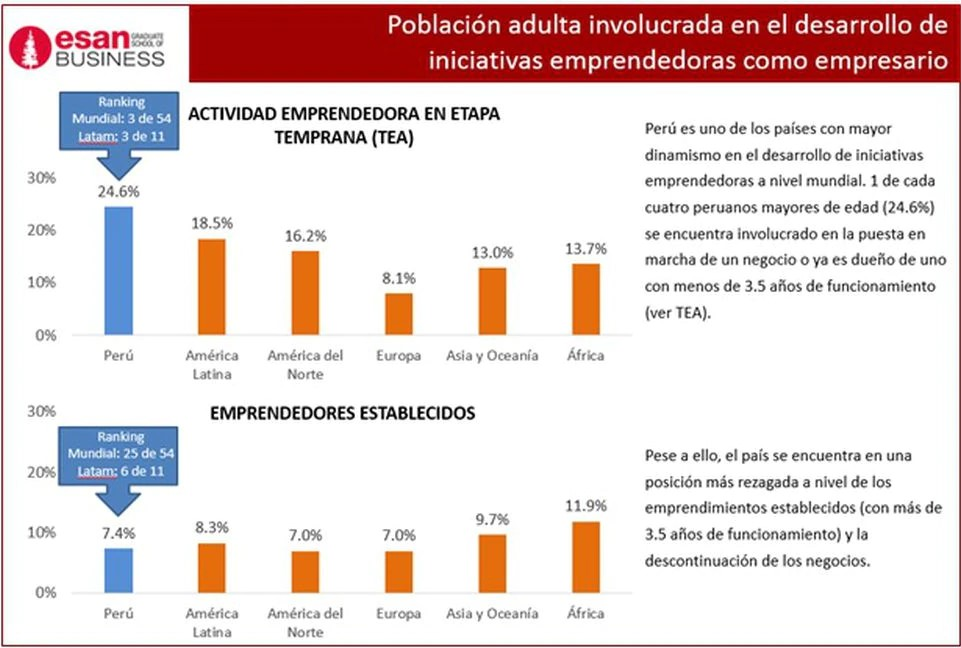
\includegraphics[width=0.7\textwidth]{1/figures/cuadro_esan.jpg}
		\caption[Resultados y ratios obtenidos en la encuesta por GEM y ESAN]{Resultados y ratios obtenidos en la encuesta por GEM y ESAN. Fuente: \cite{cr_gestion2018emprend}}
		\label{1:fig}
	\end{center}
\end{figure}

Estos resultados desfavorables tienen como base el ecosistema poco beneficioso para los emprendimientos que permitan su establecimiento en el entorno nacional, con condiciones asociadas al acceso de financiamiento, políticas gubernamentales que alienten la implementación de Innovación y Desarrollo en las empresas, acceso a infraestructura física y asesoría a nivel comercial y profesional, como sostiene el investigador del equipo GEM Perú Carlos Guerrero \parencite{cr_gestion2018emprend}. La Asociación de Emprendedores de Perú (ASEP) afirma, asimismo, que en la región solo se invierte el 1.5\% del PIB en actividades de ciencia, tecnología e innovación, y las limitaciones son dadas por barreras burocráticas ejercidas por el Gobierno y el sector privado \parencite{cr_aep2018emprend}. En adición a esto, otras razones que representan barreras para emprender son la falta de conocimientos en la iniciación de un negocio, su tramitación, la fuente de financiamiento del proyecto o búsqueda de inversionistas, la cultura, la falta de fomento de emprendimiento y la falta de una red de contactos \parencite{cr_sandoval_barreras}.

Ante estas limitaciones, en la actualidad muchos emprendedores se ven forzados a mostrar sus proyectos al público en la Internet con el fin de captar personas interesadas en ayudarlos en el financiamiento de estos. Por ello, se han creado plataformas web con el fin de permitir la interacción entre los proyectos publicados en un determinado tiempo, el cual puede variar entre 30 y 120 días, y la comunidad en general que desee colaborar con una cantidad de dinero para su financiamiento. El sitio web solo servirá para mostrar los proyectos presentados a detalle por los creadores y la promoción de estos al público. La idea es que, al término de este plazo de tiempo, el proyecto sea financiado y se logre convertir en una realidad. A esta práctica se le conoce como crowdfunding \parencite{cr_uc_crowdfunding}.

En Latinoamérica, son muy pocos los países los que se incorporan en el crowdfunding, entre los principales se destacan Chile, México, Argentina y Brasil. Sin embargo, el modelo funciona distinto a países de Norteamérica y Europa debido a la cultura diferente y resistencia a su implementación por la poca confianza en el éxito de los proyectos. En los países mencionados, se encontró que los proyectos audiovisuales, a pesar de encontrarse en desventaja que en sus pares europeos y norteamericanos, se estrenaron 4,135 títulos extranjeros en la región iberoamericana frente a 791 propios, de los cuales 162 fueron obras brasileñas y 131, argentinas, en el año 2015. Estas estadísticas se apoyan con el incremento de aperturas de salas de cines en nuestra región en las dos últimas décadas. Los factores principales: el apoyo de gobiernos latinoamericanos, la masificación de las comunicaciones digitales y por ende, la participación activa de usuarios en redes sociales y el papel protagónico que toma el crowdfunding para apoyar estos proyectos (22,179 proyectos financiados con éxito en Kickstarter con más de 1 millón de dólares de recaudación en el 2017) \parencite{cr_lopezgolan2017crowdfunding}. Asimismo, en los últimos años se decidió seguir una manera muy similar a los modelos de Estados Unidos, basados en la creación de campañas de un emprendedor para obtener fondos para sus ideas con la moneda norteamericana pero limitados a las leyes económicas de cada país \parencite{cr_sl_crowdfundlatam}.


En el caso de nuestro país, el crowdfunding sí existe y es apoyada por universidades y organizaciones sin fines de lucro, cuyo objetivo es generar empresas comerciales que aumenten la calidad de vida en la comunidad, además de convertir a las personas en socios financieros \parencite{cr_fernandezbedoya2020colecoperu}. Esta actividad es parte de uno de los 4 grupos básicos de economía colaborativa: el financiamiento colaborativo \parencite{cr_stokes2014coleco}.

Entre los sitios web más conocidos de crowdfunding están Kickstarter e Indiegogo. Kickstarter, desde su inicio en 2009, es una plataforma de financiamiento de proyectos creativos de todo tipo, los cuales incluyen películas, juegos, música, arte, diseño y tecnología. Actualmente, se han registrado más de 162 mil proyectos realizados, 16 millones de contribuyentes y 4,3 miles de millones de dólares fondeados \parencite{cr_kickstarter_about}. La plataforma utiliza un modelo de financiamiento llamado “todo o nada”, el cual consiste en que si un proyecto no alcanza su meta de financiamiento en un determinado plazo de tiempo, no se realiza ninguna transacción de fondos \parencite{cr_kickstarter_founding}. Si bien los patrocinadores apoyan estos proyectos por motivos personales y distintos para hacerlos realidad, ellos no obtienen la propiedad o los ingresos de los proyectos que financian, sino que los creadores conservan la totalidad de su trabajo \parencite{cr_kickstarter_press}.

Para los proyectos tecnológicos, en contraste, la ratio de éxito es uno de los más bajos de las categorías existentes (20\%) solo por delante de Artesanía y Periodismo, como se aprecia en la Figura \ref{1:fig2}.
\begin{figure}[h]
	\begin{center}
		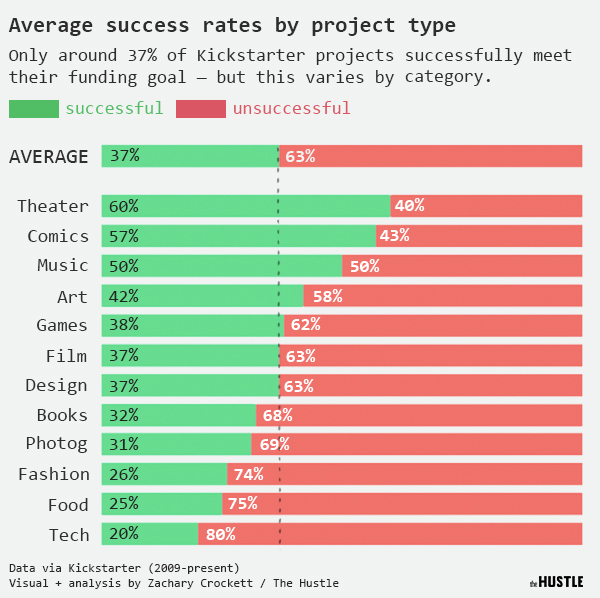
\includegraphics[width=0.6\textwidth]{1/figures/kickstarter_success_rate_2009_2019.jpg}
		\caption[Ratio de éxito de proyectos en Kickstarter desde 2009 hasta 2019 (Febrero)]{Ratio de éxito de proyectos en Kickstarter desde 2009 hasta 2019 (Febrero). Fuente: \cite{cr_hustle2019successrate}}
		\label{1:fig2}
	\end{center}
\end{figure}


Ya existen estudios previos para predecir la probabilidad de éxito de financiamiento para este tipo de proyectos utilizando técnicas de Aprendizaje Automático. Sin embargo, la mayoría de los modelos predictivos propuestos no arrojan resultados con exactitud muy alta ya que su rango varía entre 60 y 70\%. Esto conlleva a generar imprecisión para pronosticar confiablemente el éxito de financiamiento de estos proyectos de tecnología. Para el presente trabajo de tesis, se creó un modelo predictivo alimentado de datos históricos de la plataforma para estimar el estado final de financiamiento de un proyecto aleatorio, así como su probabilidad de éxito. 



\section{Formulación del Problema}
Para la formulación de los problemas de la presente investigación, se elaboró un «árbol de problemas» (véase Anexo \ref{anexo1}).

\subsection{Problema General}
\newcommand{\ProblemaGeneral}{
Bajo rendimiento de modelos de Aprendizaje Automático según sus métricas de evaluación para predecir estado de financiamiento de proyectos de tecnología. 
}
\ProblemaGeneral
\subsection{Problemas Espec\'{i}ficos}
\newcommand{\Pbone}{
Presencia de data desbalanceada.
}
\newcommand{\Pbtwo}{
Carencia de datos en variables de algunos proyectos.
}
\newcommand{\Pbthree}{
Información irrelevante considerada para entrenamiento de modelos.
}
\newcommand{\Pbfour}{
Parámetros no ajustados de modelos.
}
\newcommand{\Pbfive}{
Sobreajuste de aprendizaje de modelos y clasificación incorrecta de clases del estado final de financiamiento (exitoso o fracasado).
}
\newcommand{\Pbsix}{
Falta de herramientas predictivas para ayudar a creadores de proyectos en la toma de decisiones.
}

\begin{itemize}
	\item {\Pbone}
	\item {\Pbtwo}
	\item {\Pbthree}
	\item {\Pbfour}
	\item {\Pbfive}
	\item {\Pbsix}
\end{itemize}

\section{Objetivos de la Investigación}
Para la formulación de los objetivos de la presente investigación, se elaboró un «árbol de objetivos» (véase Anexo \ref{anexo2}) 
\subsection{Objetivo General}
\newcommand{\ObjetivoGeneral}{
Construir modelo de Aprendizaje Automático para predecir el estado de financiamiento de proyectos de tecnología.
}
\ObjetivoGeneral
\subsection{Objetivos Espec\'{i}ficos}
\newcommand{\Objone}{
Utilizar técnicas de Machine Learning para trabajar con data desbalanceada.
}
\newcommand{\Objtwo}{
Imputar datos faltantes o incompletos de proyectos.
}
\newcommand{\Objthree}{
Definir información relevante para entrenamiento de modelos.
}
\newcommand{\Objfour}{
Ajustar parámetros de modelos.
}
\newcommand{\Objfive}{
Evitar sobreajuste de aprendizaje del modelo y clasificación incorrecta de clases del estado final de financiamiento (exitoso o fracasado).
}
\newcommand{\Objsix}{
Ofrecer herramienta analítica y predictiva a creadores de proyectos para ayudar en la toma de decisiones.
}

\begin{itemize}
	\item {\Objone}
	\item {\Objtwo}
	\item {\Objthree}
	\item {\Objfour}
	\item {\Objfive}
	\item {\Objsix}
\end{itemize}

\section{Justificación de la Investigación}

\subsection{Teórica}
Esta investigación se basa en crear un modelo de Aprendizaje Automático que sea aplicable a proyectos de tecnología de la plataforma Kickstarter por presentar bajas performances en antecedentes.

\subsection{Práctica}
Al culminar la investigación, se ofrecerá un modelo predictivo confiable que ayude a los emprendedores en la toma de decisiones respecto a sus proyectos a partir del insight obtenido de los resultados que deriven a la manipulación de los datos de entrada.

\subsection{Metodológica}
Se creará un modelo predictivo a partir de las variables finales seleccionadas, previa limpieza de datos. Luego, será entrenado y evaluado por las métricas correspondientes. Finalmente, se lanzará una versión de prueba que reciba datos de entrada para predecir la viabilidad de un proyecto de tecnología.

\section{Delimitación del Estudio}

\subsection{Espacial}
Para la presente investigación, se considerará el territorio de los Estados Unidos ya que tanto la campaña del proyecto a servir para la investigación como los datos fuentes de proyectos relacionados financiados previamente, que servirán para la elaboración del modelo predictivo, se encuentran en dicho país.

\subsection{Temporal}
El periodo de tiempo abarcará desde el año 2009, fecha en el cual se tiene registrado los primeros conjuntos de datos de proyectos en Kickstarter hasta el mes de agosto del año 2019, últimos registros descargados hasta el inicio del presente trabajo.

\subsection{Conceptual}
La presente investigación consistirá en la implementación de un modelo predictivo del estado de financiamiento de un proyecto tecnológico en Kickstarter basado en técnicas y conceptos de Aprendizaje Automático, previamente evaluando cuál de todas las existentes genera un mejor desempeño para su uso y análisis de resultados.

\section{Hipótesis}

\subsection{Hipótesis General}
\newcommand{\HipotesisGeneral}{
El modelo propuesto de Aprendizaje Automático predice el estado de financiamiento de proyectos de tecnología.
}
\HipotesisGeneral
\subsection{Hipótesis Específicas}
\newcommand{\Hone}{
Las técnicas de Machine Learning ayudan a los modelos a trabajar con data desbalanceada.
}
\newcommand{\Htwo}{
Los datos faltantes o incompletos de proyectos son imputados.
}
\newcommand{\Hthree}{
Se considera solo información relevante para entrenamiento de modelos.
}
\newcommand{\Hfour}{
Los parámetros de los modelos están ajustados.
}
\newcommand{\Hfive}{
Se evita el sobreajuste de aprendizaje del modelo y éste clasifica correctamente las clases del estado final de financiamiento (exitoso o fracasado).
}
\newcommand{\Hsix}{
Se ofrece herramienta analítica y predictiva para ayudar a los creadores de proyectos en la toma de decisiones.
}
\begin{itemize}
	\item \Hone
	\item \Htwo
	\item \Hthree
	\item \Hfour
	\item \Hfive
	\item \Hsix
\end{itemize}

\subsection{Matriz de Consistencia}
A continuación se presenta la matriz de consistencia elaborada para la presente investigación (véase Anexo \ref{anexo3}).


\chapter{MARCO TEÓRICO}
\section{Antecedentes de la investigación}
En esta sección se presentarán diversos trabajos de investigación basados en la predicción de éxito o fracaso de campañas en Kickstarter o plataformas similares y el análisis de estas utilizando conjunto de datos de la propia plataforma o almacenadas en otros repositorios, con sus variables respectivas. En la mayoría de casos consideraron variables básicas que se obtienen del repositorio de las plataformas de crowdfunding, en otros casos consideraron variables cualitativas basadas en texto y descripción de proyectos, y en otros antecedentes usaron nuevas técnicas poco convencionales como el Aprendizaje Profundo e híbridos de modelos para obtener los mejores resultados posibles.
Asimismo, a continuación se presenta un cuadro resumen (véase Anexo \ref{anexo4}) de lo que se presenta en esta sección.

\subsection{Primer antecedente: «Supervised Learning Model For Kickstarter Campaigns With R Mining» \citep*{pr_kamath2018suplearn}}
\citeauthor{pr_kamath2018suplearn} realizaron un artículo de investigación el cual fue publicado en la revista «International Journal of Information Technology, Modeling and Computing» en el año 2018. Este fue titulado \citetitle{pr_kamath2018suplearn} la cual traducida al español significa «Modelo de aprendizaje supervisado para campañas de Kickstarter con R Mining».

\subsubsection{Planteamiento del Problema y objetivo}
Kickstarter actualmente es la plataforma web basado en crowdfunding más grande existente. Sin embargo, no todas las campañas que se encuentran en su portal son exitosas. Algunos trabajos previos citados en este artículo citan que el lenguaje usado en las campañas alcanza el poder predictivo de 58.86\%, es decir, la descripción semántica de un proyecto ayuda considerablemente en la predicción de éxito debido a que muchos patrocinadores se fijan en la calidad presente en una campaña antes de invertir.  Sin embargo, es dejada de lado en muchos trabajos de investigación destinados a la predicción de éxito de financiamiento, así como también las interacciones de un proyecto en redes sociales. Para el tiempo en que este artículo fue publicado, el nivel de exactitud de los modelos predictivos ya existentes bordeaba por el 68\% como el descrito anteriormente

Ante esto, autores desarrollaron un sistema con técnicas de Aprendizaje Automático usando el entorno R aplicada a conjunto de datos de campañas en Kickstarter para clasificar proyectos entrenando diferentes clasificadores en esta data y predecir con un alto nivel de exactitud.

\subsubsection{Técnicas empleadas por los autores}
Los autores elaboraron 5 modelos clasificadores para la investigación: Árbol de decisión, Bosque Aleatorio, Red Neuronal Artificial, Vecino K más cercano, y Naïve Bayes. Se consideraron como variables para estos modelos al nombre del proyecto, URL del proyecto, descripción del proyecto, categoría, sub-categoría, número de patrocinadores, monto total patrocinado, meta de financiación, fecha de lanzamiento del proyecto, duración del proyecto, número de actualizaciones, número de recompensas, si el proyecto cuenta con video, localización del proyecto, y creador del proyecto.

\subsubsection{Metodología empleada por los autores}
En primer lugar, se analizó y definió el problema. A continuación, se recolectaron 120 proyectos de Kickstarter a través de su URL. Luego, las variables categóricas fueron transformadas en numéricas como parte del pre-procesamiento. Esto permitió realizar extracción y exploración del conjunto final mediante estadísticas descriptivas con paquetes de R. Una vez analizado los datos, se procedió a elaborar los modelos clasificadores y finalmente, con la matriz de confusión, se seleccionó el mejor de ellos evaluándolos mediante la exactitud.

\subsubsection{Resultados obtenidos}
Bajo la métrica de exactitud, el mejor de los 5 modelos clasificadores construidos fue la Red Neuronal, con un valor de 0.94.


\subsection{Segundo antecedente: «Predicting Success in Equity Crowdfunding» \citep*{pr_beckwith2016predcrowd}}
\citeauthor{pr_beckwith2016predcrowd} realizó un artículo de investigación el cual fue publicado en la revista «Joseph Wharton Scholars» de la Universidad de Pensilvania en el año 2016. Este fue titulado \citetitle{pr_beckwith2016predcrowd} la cual traducida al español significa «Prediciendo el éxito en el financiamiento colectivo de acciones».

\subsubsection{Planteamiento del Problema y objetivo}
El financiamiento colectivo o crowdfunding de inversión está haciéndose cada vez más popular. Este concepto permite que los emprendedores ofrezcan algún tipo de producto o servicio como compensación por contribuciones financieras una vez que ya se tengan ventas reales o acuerdos comerciales, a diferencia por ejemplo del crowdfunding de recompensas que ofrece algo a sus patrocinadores desde la concepción del proyecto. Resulta ser muy interesante para los patrocinadores ya que no se necesita contar con un capital muy alto. A cambio, ellos recibirán algo a cambio una vez que el proyecto se realice. Este factor permite su mayor probabilidad de éxito de financiamiento al momento de darse una campaña de este tipo de crowdfunding ya que los patrocinadores pueden invertir en más de un proyecto a la vez. A partir de este punto nace la siguiente cuestión: “Dados diferentes start-ups con similares características observables, ¿qué motiva a pequeños patrocinadores a invertir en ciertos start-ups y no en otros?”.

Por ello, el objetivo del autor fue determinar la relación entre las características de una compañía determinada y su capacidad para recaudar fondos en la plataforma de financiamiento colectivo de capital AngelList.

\subsubsection{Técnicas empleadas por los autores}
El autor desarrolló un modelo de Regresión logística usando las siguientes variables: si la empresa previamente había recibido o no financiación, si la compañía cuenta con perfil en Twitter, número de veces que la compañía había sido mencionada en alguna publicación, número de veces que la compañía había sido mencionada en TechCrunch, número de personas listadas como co-fundadoras en el perfil de la compañía AngelList, si AngelList lista entre 11 y 50 empleados como tamaño de la empresa, si la compañía está ubicada en San Francisco, si entre los fundadores de AngelList al menos uno de ellos cuenta con un MBA, si entre los fundadores de AngelList al menos uno de ellos realizó sus estudios en alguna de las mejores 20 universidades de Estados Unidos, y el número de cierre del S\&P 500 el día anterior al lanzamiento de la campaña de crowdfunding de AngelList.
Este modelo se comparó con un Árbol de Decisión CART, un modelo de Naïve Bayes y una Máquina de Vectores de Soporte.

\subsubsection{Metodología empleada por los autores}
Inicialmente, se recolectaron más de 5 mil compañías de AngelList que solicitaron contribuciones financieras. De esta cantidad, se considerarons aquellas con datos completos (2,603 empresas). Luego del pre-procesamiento del conjunto final de datos, se elaboró el modelo y se evaluó el modelo mediante la exactitud, precisión, sensibilidad, puntaje F1, y área bajo la curva (AUC).

\subsubsection{Resultados obtenidos}
Bajo las métricas mencionadas, el modelo propuesto por los autores superó a los otros 3 modelos comparados en cada una, tomando como resultados 0.87 de exactitud, precisión promedio de 0.85, sensibilidad promedio de 0.88, puntaje F1 promedio de 0.86, y área bajo la curva de 0.74.


\subsection{Tercer antecedente: «Money Talks: A Predictive Model on Crowdfunding Success Using Project Description» \citep*{pr_zhou2018projectdesc}}
\citeauthor{pr_zhou2018projectdesc} realizaron un resumen de la conferencia «Twenty-first Americas Conference on Information Systems» en Puerto Rico en el año 2018. Este fue titulado \citetitle{pr_zhou2018projectdesc} la cual traducida al español significa «Money Talks: un modelo predictivo sobre el éxito del crowdfunding utilizando la descripción del proyecto».

\subsubsection{Planteamiento del Problema y objetivo}
Las investigaciones existentes de crowdfunding se centran principalmente en las variables básicas del proyecto como la categoría y la meta; sin embargo, son muy pocos estudios basados en el contenido de la información, es decir, en la descripción del mismo.

El objetivo de los autores fue estudiar la influencia y el impacto del uso de descripciones de proyectos en su éxito de financiación para predecirlo.

\subsubsection{Técnicas empleadas por los autores}
Se desarrolló un modelo de Regresión Logística usando variables previamente identificadas (meta del proyecto, duración del proyecto, si el creador tiene conección a Facebook, número de amigos en Facebook del creador, si el proyecto incluye una imagen, si el proyecto incluye un video, número de recompensas, año de lanzamiento del proyecto, categoría del proyecto) y nuevas introducidas (número de palabras en la descripción del proyecto, legibilidad de descripción del proyecto medido por Índice de niebla Gunning, ratio de positivo y negativo en descripción del proyecto, número de proyectos previamente creados y número de proyectos previamente patrocinados por el autor).

\subsubsection{Metodología empleada por los autores}
Se comenzó con la operacionalización de los constructos, es decir, cómo se consideraría la información recolectada a partir de los antecedentes en la literatura. El siguiente paso fue la recolección de información de más de 154 mil proyectos de Kickstarter entre 2009 y 2014. Y finalmente, se construyó el modelo predictivo y se comparó contra otros modelos de la base y convencionales.

\subsubsection{Resultados obtenidos}
Todos los modelos (base, convencional y propuesto) fueron evaluados por el valor-F probando en validaciones cruzadas de 3, 5 y 10 iteraciones. Bajo esta métrica, el mejor modelo fue el propuesto, alcanzando un valor-F de 71.17 con 10 iteraciones.


\subsection{Cuarto antecedente: «The Determinants of Crowdfunding Success: A Semantic Text Analytics Approach» \citep*{pr_yuan2016textanalytics}}
\citeauthor{pr_yuan2016textanalytics} realizaron un artículo de investigación el cual fue publicado en la revista «Decision Support Systems» en el año 2016. Este fue titulado \citetitle{pr_yuan2016textanalytics} la cual traducida al español significa «Los determinantes del éxito del financiamiento colectivo: Un enfoque de analítica semántica de texto».

\subsubsection{Planteamiento del Problema y objetivo}
Actualmente existen diversos estudios de éxito de campañas de financiamiento colectivo, la mayoría usando modelos predictivos en proyectos crowdfunding basados en recompensas y análisis de características poco profundas del lenguaje en descripción de los proyectos (por ejemplo, número de palabras, errores ortográficos, etc) así como en la implementación de métodos de Aprendizaje Automático.

Como propuesta alterna, los autores construyeron un marco de trabajo basado en análisis de texto que pueda extraer semánticas de descripciones textuales de proyectos para predecir sus resultados de recaudación de fondos.

\subsubsection{Técnicas empleadas por los autores}
Se creó un modelo de Bosque Aleatorio para los datos numéricos, y POS Tag Stemming más modelo DC-LDA más características tópicas para los datos textuales. Esta arquitectura se comparó con otros modelos en la literatura de la publicación.

\subsubsection{Metodología empleada por los autores}
Se recolectaron 500 proyectos de 2 webs chinas sobre crowdfunding cada una. Luego, se construyó el framework de análisis textual. A continuación, se desarrolló un modelo DC-LDA para una extracción más efectiva de las características tópicas a partir de las descripciones. Y finalmente, se realizó un análisis empírico para identificar características discriminatorias que influye en el éxito de la recaudación de fondos.

\subsubsection{Resultados obtenidos}
Para los datos numéricos, la mejor performance se obtuvo evaluando el modelo con la sensibilidad para el Random Forest (0.98 en la segunda data); mientras que para los datos textuales, el modelo DC-LDA (al ser comparado con el LDA normal) obtuvo un puntaje F1 de 0.91.


\subsection{Quinto antecedente: «Will your Project get the Green light? Predicting the success of crowdfunding campaigns» \citep*{pr_chen2015predcrowd}}
\citeauthor{pr_chen2015predcrowd} realizaron un resumen de la conferencia «Pacific Asia Conference on Information Systems (PACIS) 2015» en New York, Estados Unidos. Este fue titulado \citetitle{pr_chen2015predcrowd} la cual traducida al español significa «¿Tu proyecto obtendrá la luz verda? Prediciendo el éxito de campañas de financiamiento colectivo».

\subsubsection{Planteamiento del Problema y objetivo}
Desde el surgimiento de campañas de financiamiento colectivo en sitios web así como estudios de estos casos, la mayoría de estos presentan problemas en la predicción de éxito de una campaña por distintas casuísticas ya que suelen enfocarse en aquellos concluídos. ¿Será posible desarrollar una técnica efectiva para predecir si una campaña será exitosa o no en diferentes momentos de tiempo de las campañas de crowdfunding?

Para responder esta interrogante, los autores desarrollaron una técnica efectiva para predecir si una campaña de crowdfunding tendrá éxito o fracasará a través de extracción y posterior uso de características estáticas y dinámicas.

\subsubsection{Técnicas empleadas por los autores}
Los autores construyeron una serie de 8 modelos de Bosque Aleatorio para diferentes etapas (puntos de tiempo) de la campaña desde el día 0 hasta el día 7.

\subsubsection{Metodología empleada por los autores}
Se recolectaron más de 4 mil proyectos de Kickstarter obtenido directamente desde el sitio, así como con ayuda de la página web Kickspy, entre el primer y último día de abril del 2014. Una vez pre-procesada la data, se extrajeron las características para la tarea de predicción de objetivos. Luego, estas características se clasificaron en 5 categorías: características intrínsecas, mecanismo financiero, calidad y sentimiento del contenido, interacción social y efecto de progresión, en donde las 3 primeras + interacción social corresponden a un nuevo grupo asignado como «características estáticas», mientras que la última + interacción social se asignó como «características dinámicas». Ambos nuevos conjuntos agrupados finalmente fueron entrenados con la serie de modelos para diferentes etapas.

\subsubsection{Resultados obtenidos}
Se comparó la serie de modelos propuestos considerando todas las características con modelos que solo consideraban algunas, así como también comparado con uno de la literatura. El resultado final de la evaluación medidos por la exactitud determinó que la primera opción mencionada logró la mejor performance, con un valor de 0.8467.


\subsection{Sexto antecedente: «Project Success Prediction in Crowdfunding Environments» \citep*{pr_li2016predcrowd}}
\citeauthor{pr_li2016predcrowd} realizaron un resumen de la conferencia «WSDM’ 16 Proceedings of the Ninth ACM International Conference on Web Search and Data Mining» en San Francisco (2016). Este fue titulado \citetitle{pr_li2016predcrowd} la cual traducida al español significa «Predicción de éxito de un proyecto en ambientes de financiamiento colectivo».

\subsubsection{Planteamiento del Problema y objetivo}
Durante la última década se han elaborado una serie de modelos de clasificación que permitan pronosticar con cierto nivel de exactitud si algunos proyectos de financiamiento colectivo tendrán éxito o no. Sin embargo, el hecho de estimar si esto ocurrirá durante el plazo dado de la campaña no puede proporcionar una guía adecuada a los patrocinadores que desean invertir en proyectos populares. Es entonces que se cuestiona la posibilidad de predecir el éxito de campañas en sitios web de crowdfunding como Kickstarter considerando características obtenidas durante la operación de la campaña.

Para ello, los autores formularon la predicción del éxito del proyecto como un problema de análisis de supervivencia y aplicar el enfoque de regresión censurada.

\subsubsection{Técnicas empleadas por los autores}
Los autores desarrollaron 2 modelos para evaluar la regresión censurada: 1 modelo de distribución logística y 1 de distribución log-logística. Para comparar con sus modelos, también se elaboraron otros métodos para manejar observaciones censuradas, mencionados en la literatura como Cox, Regresión Tobit, estimación Buckley-James e Índice de Concordancia Boosting (BoostCI).

\subsubsection{Metodología empleada por los autores}
Inicialmente, se recolectaron más de 27 mil proyectos de Kickstarter entre diciembre del 2013 y junio del 2014 para la data estática, a los cuales se removieron los cancelados, suspendidos o con menos de 1 patrocinador y monto prometido de \$100. Asimismo, para la data dinámica se capturaron más de 106 mil tweets de Twitter que contenían el enlace rápido hacia la página de Kickstarter. Una vez obtenidos los conjuntos de datos, se pre-procesaron para finalmente elaborar los modelos predictivos.

\subsubsection{Resultados obtenidos}
Como resultados de las múltiples pruebas en los modelos, en los cuales los autores experimentaron distintas combinatorias con la data estática y la dinámica, así como agregando y desagregando proyectos fracasados, se obtuvo que el modelo de Regresión log-logística evaluado con el área bajo la curva (AUC) presentó mejor performance que el resto en 3 de las 4 combinatorias, alcanzando su mejor nivel en el conjunto de datos que combina data estática, dinámica, de características de proyectos transcurridos los primeros 3 días y con proyectos fracasados, con un puntaje Survival AUC de 0.9030.


\subsection{Séptimo antecedente: «Effect of Social Media Connectivity on Success of Crowdfunding Campaigns» \citep*{pr_kaur2017socmedcrowd}}
\citeauthor{pr_kaur2017socmedcrowd} realizaron un artículo de investigación el cual fue publicado en la revista «Procedia Computer Science» en el año 2017. Este fue titulado \citetitle{pr_kaur2017socmedcrowd} la cual traducida al español significa «Efecto de conectividad en medios sociales en éxito de campañas de financiamiento colectivo».

\subsubsection{Planteamiento del Problema y objetivo}
Los proyectos de crowdfunding, así como los proyectos lanzados en sitios dedicados a esto, han crecido exponencialmente en los últimos años. Los medios sociales desempeñan un papel importante en la difusión de palabras sobre una campaña y en la obtención de fondos con éxito. Después de lanzarse una campaña, su éxito se define por la interacción social de los creadores en la plataforma y en las redes sociales. Además, el tamaño de la red social del creador y su presencia en línea motiva a los patrocinadores a participar y financiar el proyecto. Partiendo de esta premisa, se busca conocer el impacto de la conectividad con las redes sociales y las interacciones sociales en el rendimiento del crowdfunding.

Para ello, los autores plantearon el desarrollo de un modelo predictivo que comprenda las características de la campaña y sumado a eso, la información sobre la conectividad con las diversas redes sociales como Facebook y Twitter.

\subsubsection{Técnicas empleadas por los autores}
Los autores propusieron un modelo de Regresión Logística, el cual compararon con algunos enunciados en sus antecedentes como Naïve Bayes, J48 y Bosques Aleatorios.

\subsubsection{Metodología empleada por los autores}
Se recolectaron 2 tipos de conjuntos de datos: el primero obtenido desde Kickstarter en el mes de Abril del 2014, con más de 4 mil campañas; mientras que el segundo a través del perfil del creador vinculado a redes sociales. El primer conjunto comprendió las variables de categoría, tipo de divisa, monto de la meta, monto prometido, número de recompensas, duración de la campaña en días, y el estado final de financiamiento (exitoso o fracasado). Por el lado del segundo conjunto, además de obtener marcas de hacia qué redes sociales el creador se conecta, mediante el enlace se extrajeron más de 19 mil tweets en el que se promocionaron las campañas gracias a la API de Twitter.

Una vez armados los conjuntos de datos, se creó el modelo propuesto y se comparó con las bases de referencia usando como métrica principal la exactitud. Previo a este paso, todas las variables consideradas se evaluaron en una matriz de correlaciones con el valor de “exitoso” de la variable dependiente.

\subsubsection{Resultados obtenidos}
Culminados los experimentos de la selección de variables en la matriz de correlaciones, así como la ejecución del modelo de Regresión Logística, la exactitud de este alcanzó un valor de 0.767 para un subconjunto de 66\% de entrenamiento y de 34\% de prueba, indicando así que la conectividad a medios sociales e interacciones en ellos influye en la predicción de éxito de la campaña. Asimismo, evaluando también con precisión y sensibilidad promedio, el ratio alcanzó 0.768 y 0.767 respectivamente.


\subsection{Octavo antecedente: «Prediction of Crowdfunding Project Success with Deep Learning» \citep*{pr_yu2018deeplearning}}
\citeauthor{pr_yu2018deeplearning} realizaron un resumen de la conferencia «2018 IEEE 15th International Conference on e-Business Engineering (ICEBE)» del 12 al 14 de octubre del 2018 en Xi'an, China. Este fue titulado \citetitle{pr_yu2018deeplearning}, la cual traducida al español significa «Predicción del éxito de proyecto de financiamiento colectivo con Aprendizaje Profundo».

\subsubsection{Planteamiento del Problema y objetivo}
Debido al aumento dramático de la actividad de financiamiento colectivo en los últimos años, en el cual tanto creadores como patrocinadores participan, son más las campañas que buscan alcanzar su objetivo. Sin embargo, según el análisis empírico, solo la tercera parte lo logra. La incógnita que rodea a esta situación es la posibilidad de elaborar un modelo predictivo de éxito en proyectos de Kickstarter utilizando distintas técnicas al Aprendizaje Automático.

Por ello, los autores plantean como objetivo el desarrollo de un modelo que prediga el éxito del proyecto de crowdfunding con Aprendizaje Profundo usando registros históricos de campañas en Kickstarter.

\subsubsection{Técnicas empleadas por los autores}
Los autores elaboraron un modelo basado en un Perceptrón Multicapa (MLP), alimentado por 6 variables visibles de la campaña (metadata). Además, sus resultados se compararon con otros modelos considerados en sus antecentes como Bosques aleatorios, AdaBoost, Máquina de vectores de soporte, Árboles de decisión, Regresión logística y Naïve Bayes.

\subsubsection{Metodología empleada por los autores}
Se recolectaron más de 378 mil campañas de Kickstarter entre Mayo 2009 y Marzo 2018, recopilados retrospectivamente desde Kaggle. A continuación, realizaron análisis exploratorio de los datos para entender la data y seleccionar variables, y finalmente construyeron un modelo, el cual se comparó sus resultados con los de otros modelos.

\subsubsection{Resultados obtenidos}
Para comparar los resultados del modelo propuesto con los antecedentes, se tomaron en cuenta como métricas la exactitud y el área bajo la curva (AUC). De acuerdo a ellas, para ambos escenarios se lograron mejor performance, con una exactitud de 0.9320 y un área bajo la curva de 0.9323 frente al mejor modelo de los antecedentes, Bosques Aleatorios, que obtuvo como resultados 0.9293 y 0.9272 para las mismas métricas respectivamente.

\subsection{Noveno antecedente: «Estimating the Days to Success of Campaigns in Crowdfunding: A Deep Survival Perspective» \citep*{pr_jin2019dayssuccess}}
\citeauthor{pr_jin2019dayssuccess} realizaron un resumen de la conferencia «The 33rd AAAI Conference on Artificial Intelligence (AAAI'2019)» del 27 de enero al 1 de febrero del 2019 en Honolulu, Estados Unidos. Este fue titulado \citetitle{pr_jin2019dayssuccess} la cual traducida al español significa «Estimación de días de éxito de campañas en financiamiento colectivo: Una perspectiva de supervivencia profunda».

\subsubsection{Planteamiento del Problema y objetivo}
Dado el incremento de actividad en campañas de crowdfunding en sitios como Kickstarter o Indiegogo, los estudios sobre este tema también han ido de la mano. Sin embargo, la mayoría de investigaciones se enfocan en predecir el ratio de éxito de financiamiento en una campaña. El reto de predecir el tiempo de duración es más complicado porque se ve afectada por la variabilidad de la metadata y los comentarios del proyecto, resultando un alto nivel de fracaso (60\%) en la financiación de proyectos.

Los autores plantean la predicción de la fecha exacta de finalización de una campaña, así como controlar la distribución de patrocinios conforme a la evolución del tiempo.

\subsubsection{Técnicas empleadas por los autores}
Se elaboró un modelo Seq2seq (encoder + decoder) con previos multifacéticos (SMP) para la distribución de patrocinios y el tiempo de éxito, así como también un modelo evolutivo lineal para mantener el cambio de las distribuciones de patrocinios.

\subsubsection{Metodología empleada por los autores}
Se recolectó más de 14 mil proyectos de Indiegogo con información estática (descripción de campaña, descripción de las recompensas, categoría de la campaña, tipo del creador, duración declarada de financiación, meta declarada prometida, número de recompensas, precio máximo/mínimo/promedio de recompensas, plazo máximo/mínimo/promedio de entrega) y dinámica (comentarios), luego se definió el problema estudiado. A continuación, se introdujo los detalles técnicos de SMP, el conjunto pre-procesado de entrada, la arquitectura SMP, los previos multifacéticos y por último, el método de entrenamiento del modelo.

\subsubsection{Resultados obtenidos}
Respecto a la predicción de distribución de patrocinios, y evaluando mejor con RECM, los modelos propuestos de SMP fueron los más efectivos (0.135 para 70\% de ratio de partición) para el Encoder.
Respecto a la predicción del tiempo de éxito, los modelos propuestos de SMP (el mejor con 0.96 para 50\% de ratio de partición) fueron mejores que modelos de referencia para el Decoder.

\subsection{Décimo antecedente: «Success Prediction on Crowdfunding with Multimodal Deep Learning» \citep*{pr_cheng2019deeplearning}}
\citeauthor{pr_cheng2019deeplearning} realizaron un resumen de la conferencia «The Twenty-Eighth International Joint Conference on Artificial Intelligence (IJCAI-19)» del 10 al 16 de agosto del 2019 en Macao, China. Este fue titulado \citetitle{pr_cheng2019deeplearning} la cual traducida al español significa «Predicción del éxito en financiamiento colectivo con Aprendizaje Profundo Multimodal».

\subsubsection{Planteamiento del Problema y objetivo}
La mayoría de los enfoques de predicción existentes aprovechan solo la modalidad dominada por el texto a pesar de existir más información en los perfiles de los proyectos, como por ejemplo, metadatos e imágenes. A estos últimos se han realizado poco trabajo para evaluar sus efectos hacia la predicción del éxito. Además, la metainformación ha sido explotada en muchos enfoques existentes para mejorar la precisión de la predicción. Sin embargo, esta generalmente se limita a la dinámica después de la publicación de los proyectos, haciendo que tanto los creadores del proyecto como las plataformas no puedan predecir el resultado de manera oportuna. Se carecen estudios basados en distintas modalidades más allá de la metainformación.

El objetivo de los autores es construir esquemas avanzados de redes neuronales que combinan información de diferentes modalidades para predecir el estado de financiamiento del proyecto usando solo información pre-publicación.

\subsubsection{Técnicas empleadas por los autores}
Debido a que los autores construyeron un modelo apilado de 3 modelos para cada modalidad, cada una se distribuyó de la siguiente manera: un modelo de Máquina de Vectores de Soporte (SVM) para la metainformación; la Red Neuronal Convolucional (CNN) pre-entrenada de 16 capas VGG16, trabajando junto con la Bolsa de Palabras Visuales (BoVW) para las imágenes; y la Bolsa de Palabras (BoW) trabajando junto con el método Frecuencia de Términos - Frecuencia Inversa de Documentos (TF-IDF), con modelo de incrustaciones de palabras GloVe de 300 dimensiones.

\subsubsection{Metodología empleada por los autores}
Se recolectaron más de 20 mil campañas finalizadas (exitosas o fracasadas) en Kickstarter gracias a algoritmo creado para captura de datos en la página por 2 semanas. Se descartaron proyectos previos al 2015, resultando así proyectos entre este año y el 2018. Asimismo, entre el contenido obtenido se registraron perfil textual (título, resumen, descripción del financiamiento, y riesgos/retos), imágenes (en formato jpg), categorías, meta de financiamiento, fecha de inicio y de finalización de campaña. Luego, se realizó pre-procesamiento a los subconjuntos de datos y se dividieron en 3 subconjuntos: entrenamiento (proyectos del 2015 y 2016), validación (2017) y prueba (2018). A continuación, se configuró la arquitectura del marco de trabajo del modelo Aprendizaje Profundo Multimodal y finalmente se realizaron distintos experimentos elaborando combinatorias de distintas modalidades para compararlas entre sí mediante las métricas de sensibilidad, precisión, puntaje F1 y área bajo la curva (AUC).

\subsubsection{Resultados obtenidos}
Realizando una comparación entre la base de referencia de un modelo SVM con texto, imágenes y metadata (SVM-TIM), contra el modelo propuesto (MDL-TIM) por los autores, se observó que bajo todas las métricas, con excepción de la precisión, el marco de trabajo Multimodal obtuvo mejores resultados, con 0.7505 en sensibilidad, 0.7534 en puntaje F1 y 0.8326 en área bajo la curva, frente a 0.7411, 0.7483 y 0.7411 respectivamente.
\clearpage

\section{Bases Teóricas}
\subsection{Inteligencia Artificial}

La Inteligencia Artificial es la inteligencia llevado a cabo por máquinas en las que una máquina “inteligente” ideal es un agente flexible que percibe su entorno y lleva a cabo acciones que maximicen sus posibilidades de éxito en algún objetivo \parencite{tec_poole1998machinelearning}. Este término se aplica cuando una máquina imita las funciones “cognitivas” que asocian los humanos con otras mentes \parencite{bk_russell2009intart}.

Durante la historia de la humanidad, se han seguido 4 enfoques: dos centrados en el comportamiento humano y dos enfocados en torno a la racionalidad. El enfoque centrado en el comportamiento humano se basa en una ciencia empírica, es decir, mediante experimentos que incluyen hipótesis y confirmaciones. Este enfoque nace a partir de la prueba de Alan Turing, en 1950, en la cual, el célebre matemático inglés diseñó una prueba basada en la incapacidad de diferenciar entre entidades inteligentes indiscutibles y seres humanos por parte de un computador. Si este era capaz de diferenciar y superar la prueba mientras que el humano no, se afirma que se trataba de una “máquina inteligente”. Por ello, el computador debía contar con las siguientes capacidades: procesamiento de lenguaje natural para poder comunicarse, representación del conocimiento describiendo lo que percibe de su entorno, razonamiento automático utilizando la información procesada en su interior, y aprendizaje automático para adaptarse a nuevos eventos. Si el evaluador decide incluir una señal de video para evaluar la percepción de la computadora, se dice que se está realizando la Prueba Global de Turing. Para superarla, además de las 4 anteriormente mencionadas, la computadora debe contar además con las capacidades de visión computacional para percibir objetos y robótica con el fin de manipularlos. Todas estas seis capacidades o disciplinas abarcan la mayor parte de la Inteligencia Artificial \parencite{bk_russell2004intart}.

Por el otro lado, el enfoque racional implica una combinación de ingeniería y matemáticas basándose en las “leyes del pensamiento”. Estas parten de la Grecia antigua, planteadas por grandes filósofos como Aristóteles en su intento de codificar la “manera correcta de pensar”, lo que más adelante derivó al estudio de la lógica. Más adelante, en el siglo XIX, se construyeron programas capaces de resolver problemas en notación lógica. De ahí que la tradición logista dentro del campo de la Inteligencia Artificial trata de construir sistemas inteligentes con estas capacidades. De todo lo anterior dicho respecto al enfoque racional se creó el término de un agente racional, el cual actúa intentando lograr el mejor resultado, o de existir incertidumbre, el mejor resultado esperado. Finalmente, la amplia aplicación de la Inteligencia Artificial y sus fundamentos derivan en muchas ciencias de las cuales se pueden mencionar, además de la filosofía y las matemáticas, a la economía, neurociencia, psicología, la ingeniería computacional, la teoría de control y cibernética, y hasta la lingüística \parencite{bk_russell2004intart}.

Pero, ¿cómo es surge este amplio estudio de la Inteligencia Artificial? En 1943, basándose en la fisiología básica y funcionamiento de las neuronas en el cerebro, el análisis formal de la lógica proposicional de Russell y Whitehead, y la teoría computacional de Turing, dos estudiosos en neurociencia realizaron juntos el que sería considerado primer trabajo de Inteligencia Artificial. Warren McCulloch y Walter Pitts propusieron un modelo constituido por neuronas artificiales, en el que cada una de ellas se caracterizaba por estar “activada” o “desactivada”; la del primer tipo daba como resultado a la estimulación producida por una cantidad suficiente de neuronas vecinas. Como ejemplo, mostraron que cualquier función de cómputo podría calcularse mediante alguna red de neuronas interconectadas y que todos los conectores lógicos eran capaces de ser implementados usando estructuras sencillas de red. Seis años más adelante, Donald Hebb propuso una regla de actualización de intensidades de conexiones entre las neuronas, la que actualmente se le conoce como la “regla de aprendizaje Hebbiano” vigente hasta nuestros días. En 1956, Allen Newell y Herbert Simon inventaron un programa de computación en el taller de Dartmouth de John McCarthy, que era capaz de pensar de forma no numérica, basado en el Teórico Lógico, artículo que, además, fue rechazado de ser publicado en la revista \textit{Journal of Symbolic Logic}. A pesar de ello, los trabajos de los colaboradores presentes en dicho taller se mantuvieron por 20 años más, siendo McCarthy quien acuñó el término de “Inteligencia Artificial” a este campo \parencite{bk_russell2004intart}.

En la década de los años 80, la Inteligencia Artificial dio el gran salto de formar parte de la industria, en especial, de las compañías más grandes de los países desarrollados a través de grupos especializados para la realización de investigaciones de sistemas expertos, así como en la construcción de computadoras cada vez más potentes y capaces de resolver tareas más complejas.

Actualmente, la IA cuenta con muchas aplicaciones como la Minería de Datos, el procesamiento de lenguaje natural, la robótica, los videojuegos, entre otros. Dentro de ella se pueden encontrar otras ramas como por ejemplo el Aprendizaje Automático, Visión computacional, etcétera.

\subsection{Aprendizaje Automático}
El Aprendizaje Automático (\textit{Machine Learning} por su nombre en inglés) es una rama de la Inteligencia Artificial cuyo fin es desarrollar técnicas que las computadoras pueden aprender a través de encontrar algoritmos y heurísticas que conviertan muestras de datos en programas sin necesidad de hacerlos \parencite{bk_russell2009intart}. Sus algoritmos están compuestos por muchas tecnologías, como por ejemplo Aprendizaje Profundo, Redes Neuronales y Procesamiento de lenguaje natural, utilizadas en el aprendizaje supervisado y no supervisado, las cuales operan guiadas por lecciones de información existente \parencite{gl_gartner2019ml}. La premisa básica del aprendizaje automático es construir algoritmos que puedan recibir datos de entrada y usar análisis estadísticos para predecir una salida mientras se actualizan las salidas a medida que se dispone de nuevos datos \parencite{bk_alpaydin2014ml}.

Los tres tipos de aprendizaje principales son:
\begin{itemize}
	\item \textbf{Aprendizaje supervisado}: Se trabajan con datos etiquetados buscando obtener una función que asigne una respuesta de salida adecuada, denominadas etiquetas, a partir de unos datos de entrada denominadas características \parencite{bk_zambrano2018supnosup}. Por lo general, los datos de entrada son conocidos como variables dependientes o X, mientras que los datos de salida son llamadas variables independientes o Y. Se le dice supervisado ya que el resultado depende de los datos que recibe de entrada, afectando su performance si estos son alterados.
	
	Existen dos tipos de aprendizaje supervisado (ver Figura \ref{2:fig1}). El primero es la regresión, que consiste en obtener como resultado un número específico a partir de un conjunto de variables de las características; mientras que por otra parte está la clasificación, el cual se basa en encontrar distintos patrones ocultos para clasificar los elementos del conjunto de datos en diferentes grupos \parencite{bk_zambrano2018supnosup}.
	\begin{figure}[!ht]
		\centering
		\small
		\begin{subfigure}{.5\textwidth}
			\centering
			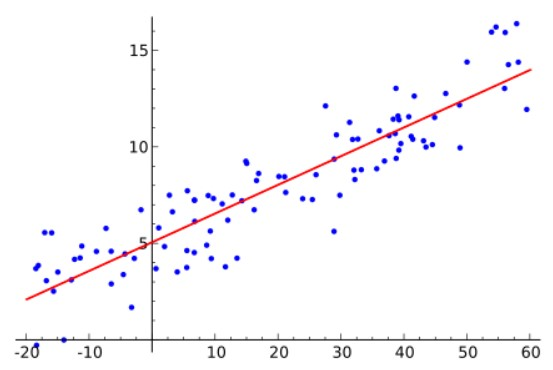
\includegraphics[width=0.75\linewidth]{2/figures/regresion.jpg}
			\caption{Regresión}
		\end{subfigure}%
		\begin{subfigure}{.5\textwidth}
			\centering
			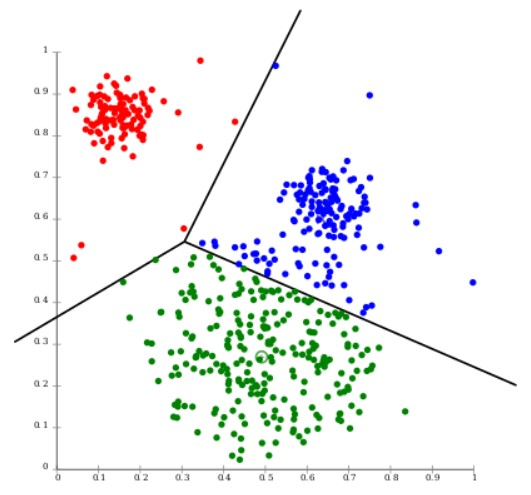
\includegraphics[width=0.65\linewidth]{2/figures/clasificacion.jpg}
			\caption{Clasificación}
		\end{subfigure}
		\caption[Ejemplo de algoritmos de regresión y clasificación]{Ejemplo de algoritmos de regresión y clasificación.\\
		Fuente: \cite{bk_zambrano2018supnosup}. \textit{¿Aprendizaje supervisado o no supervisado? Conoce sus diferencias dentro del machine learning y la automatización inteligente}.}
		\label{2:fig1}
	\end{figure}
	
	Para el segundo tipo de aprendizaje supervisado, el algoritmo más usado es el de los K Vecinos más cercanos o \textit{k-NN Nearest Neighbour} en inglés. Este se basa en la idea de que los nuevos ejemplos serán clasificados a la clase a la cual pertenezca la mayor cantidad de vecinos más cercanos del conjunto de entrenamiento más cercano a él. Sin embargo, el número k de vecinos más cercanos lo decide el usuario, de preferencia impar, para evitar ambigüedad al momento de clasificar un registro por parte del algoritmo (esto puede ocasionarse por las mismas distancias existentes entre dos o más registros). Otra variante aplicada consiste en la ponderación de cada vecino de acuerdo a la distancia entre él y el ejemplar a ser clasificado, asignando mayor peso a los más próximos \parencite{tec_sancho2018supnosup}. Para ello, se tiene la Ecuación \ref{eq:weights-KNN} y su variante en la Ecuación \ref{eq:weights-KNN_alt}:	
	%\begin{equcaption}[!ht]
	\begin{equation}\label{eq:weights-KNN}
	\phantomsection
	W_i = \frac{1}{d(x, x_i)^2}
	\end{equation}
	\myequations{Cálculo de pesos para K-NN mediante ponderación de sus distancias}
	%\caption[Cálculo de pesos para K-NN mediante ponderación de sus distancias]{Cálculo de pesos para K-NN mediante ponderación de sus distancias. Fuente: \cite{tec_sancho2018supnosup}}
	%\end{equcaption}

	%\begin{equcaption}[!ht]
	\begin{equation}\label{eq:weights-KNN_alt}
	\phantomsection
	argmax_{v \in V}\sum_{i=1…k,x_i \in v}W_i
	\end{equation}
	\myequations{Fórmula alternativa del algoritmo K-NN mediante sumatoria de pesos}
	%\caption[Fórmula alternativa del algoritmo K-NN mediante sumatoria de pesos]{Fórmula alternativa del algoritmo K-NN mediante sumatoria de pesos. Fuente: \cite{tec_sancho2018supnosup}}
	%\end{equcaption}

	Donde:
	\begin{conditions}
		x	&	ejemplo que se desea clasificar \\
		V	&	posibles clases de clasificación \\
		x_i   &  conjunto de los k ejemplos de entrenamiento más cercanos
	\end{conditions}
		
	y finalmente, la clase asignada a $x$ es aquella que verifique que la suma de los pesos de sus representantes sea la máxima, representándose en la Figura \ref{2:fig2}:
	
	\begin{figure}[h]
		\begin{center}
			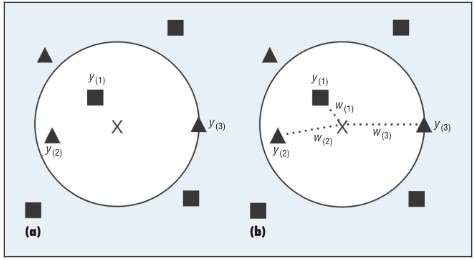
\includegraphics[width=0.55\textwidth]{2/figures/knn.jpg}
			\caption[Algoritmo de K Vecinos más cercanos con pesos ponderados]{Algoritmo de K Vecinos más cercanos con pesos ponderados.\\
			Fuente: \cite{tec_sancho2018supnosup}. \citetitle{tec_sancho2018supnosup}.}
			\label{2:fig2}
		\end{center}
	\end{figure}
	
	\item \textbf{Aprendizaje no supervisado}: A diferencia de la anterior, aquí se trabaja con datos no etiquetados para entrenar el modelo, ya que el fin es de carácter exploratorio y descriptivo de la estructura de los datos. No existen variables independientes o Y.
	
	La función es agrupar ejemplares, por lo que el algoritmo los cataloga por similitud en sus características y a partir de ahí, crea grupos o clústeres sin tener la capacidad de definir cómo es cada individualidad de cada uno de los integrantes de los mismos \parencite{bk_zambrano2018supnosup}.
	
	El algoritmo usado para este tipo de aprendizaje es el de las K medias o \textit{k-means} en inglés. Este intenta encontrar una partición de las muestras en K agrupaciones, de manera que cada ejemplar pertenezca a una de ellas de acuerdo al centroide más cercano. Si bien el valor de K es definido por el usuario, a partir de pruebas de varias iteraciones se le puede consultar al algoritmo cuál es su valor óptimo. La función para lograr esto se observa en la Ecuación \ref{eq:k-means}:
	%\begin{equcaption}[!ht]
	\begin{equation}\label{eq:k-means}
	\phantomsection
	\sum_{i}\sum_{j}\mathrm{d}(x_j^i, c_i)^2
	\end{equation}
	\myequations{Fórmula del algoritmo k-means}
	%\caption[Fórmula del algoritmo k-means]{Fórmula del algoritmo k-means. Fuente: \cite{tec_sancho2018supnosup}}
	%\end{equcaption}
	
	Donde:
	\begin{conditions}
		c_i   &  centroide de la agrupación i-ésima \\
		x_j^i   &  conjunto de ejemplos clasificados de la agrupación i-ésima
	\end{conditions}
	
	Representándose en la Figura \ref{2:fig3}, los pasos seguidos para este algoritmo comienzan con la selección de los K puntos como como centros de los grupos. Luego, se asignarán los ejemplos al centro más cercano y se calculará el centroide de los ejemplos asociados a cada grupo. Finalmente, estos dos últimos pasos se repetirán hasta que ninguno de los centros pueda ser reasignados en las iteraciones.
	\begin{figure}[h]
		\begin{center}
			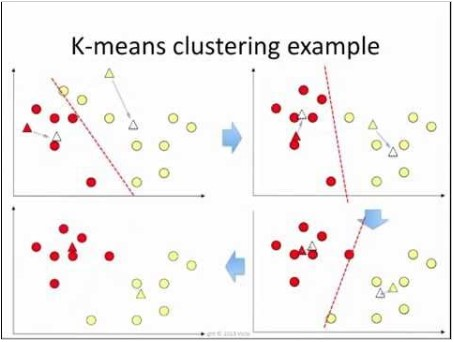
\includegraphics[width=0.50\textwidth]{2/figures/kmeans.jpg}
			\caption[Funcionamiento del algoritmo de K medias]{Funcionamiento del algoritmo de K medias.\\
			Fuente: \cite{tec_sancho2018supnosup}. \citetitle{tec_sancho2018supnosup}.}
			\label{2:fig3}
		\end{center}
	\end{figure}
		
	\item \textbf{Aprendizaje por refuerzo}: Se basa en que un agente racional puede tomar una decisión a partir de una retroalimentación llamada recompensa o refuerzo. A diferencia del Aprendizaje Supervisado, en donde el agente puede aprender solamente a partir de ejemplos dados, en este caso no basta solamente con proporcionárselos sino también de “informarle” si lo está haciendo de la manera correcta o no. Por ejemplo, un agente que intenta aprender a jugar ajedrez necesita saber que algo bueno ha ocurrido cuando gana y algo malo ha ocurrido cuando pierde. La mejor recompensa que busca al finalizar el juego es vencer al oponente, y para ello debe estudiar todos los movimientos que este haga, la posición de las fichas en el tablero, entre otros. A este conjunto se le conoce como entorno o medio ambiente \parencite{bk_russell2004intart}. Entonces, en resumen, representando en la Figura \ref{2:fig4}, y mencionando otro ejemplo, el aprendizaje por refuerzo está compuesto por un agente (Pacman) en un estado determinado (su ubicación o posición actual) dentro de un medio ambiente (el laberinto). La recompensa positiva que busca Pacman son los puntos por comer, mientras que la negativa será la de morir si se cruza con un fantasma, en base a la acción (desplazamiento a un nuevo estado) que realice \parencite{tec_merino2019aprendrefuerzo}.
	\begin{figure}[h]
		\begin{center}
			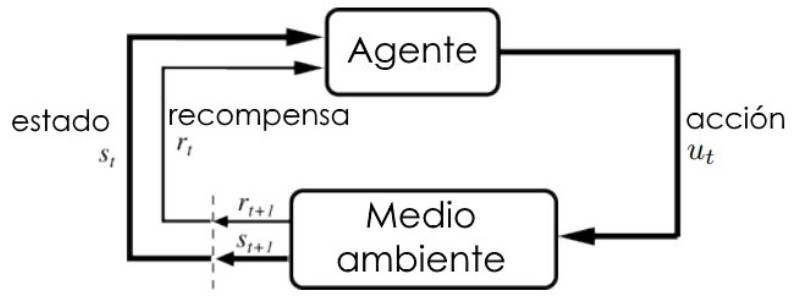
\includegraphics[width=0.60\textwidth]{2/figures/aprendizaje_refuerzo.jpg}
			\caption[Componentes del Aprendizaje por Refuerzo]{Componentes del Aprendizaje por Refuerzo.\\
			Fuente: \cite{bk_sutton2018rl}. \textit{Finite Markov Decision Processes}. (p. 48)}
			\label{2:fig4}
		\end{center}
	\end{figure}
\end{itemize}

\clearpage

\subsection{Aprendizaje Profundo}

El Aprendizaje Profundo (\textit{Deep Learning} por su nombre en inglés) es un tipo de Aprendizaje Automático que entrena a una computadora para realizar tareas hechas por los seres humanos, desde la identificación de imágenes hasta predecir y reconocer el lenguaje humano. El Aprendizaje Profundo configura parámetros básicos acerca de los datos y entrena a la computadora para que aprenda por su cuenta reconociendo patrones mediante el uso de múltiples capas de procesamiento \parencite{gl_sas_deeplearning}. Se basa en teorías acerca de cómo funciona el cerebro humano \parencite{tec_banafa2019deeplearning}.

La principal diferencia con el Aprendizaje Automático es que el Aprendizaje Profundo se basa en la extracción de características y clasificación al mismo tiempo luego de recibir una entrada, algo que en la primera técnica ocurre por separado, como se aprecia en la Figura \ref{2:fig5}.
\begin{figure}[!ht]
	\begin{center}
		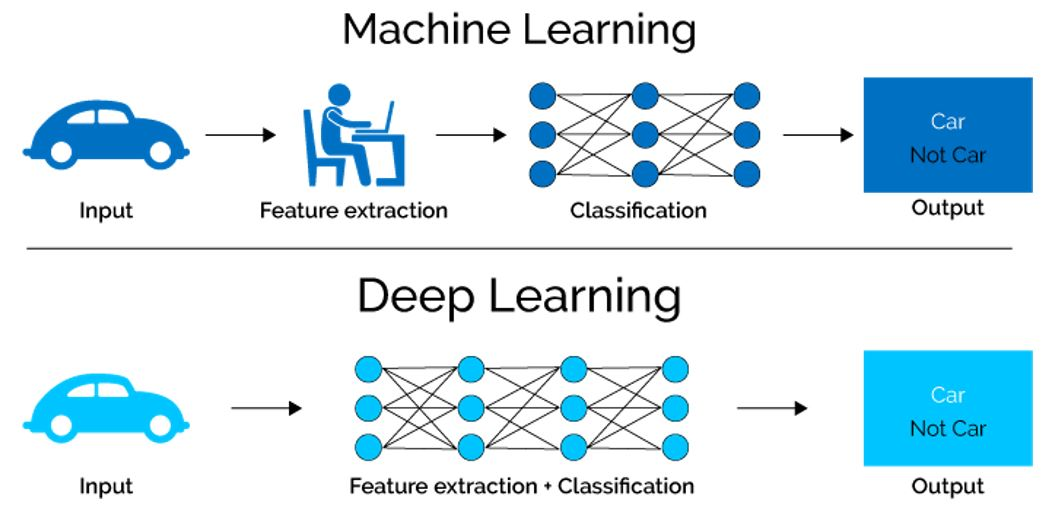
\includegraphics[width=0.70\textwidth]{2/figures/deeplearning_machinelearning.jpg}
		\caption[Diferencia entre Aprendizaje Automático y Aprendizaje Profundo]{Diferencia entre Aprendizaje Automático y Aprendizaje Profundo.\\
		Fuente: \cite{tec_cook2018deeplearning}. \textit{Most Popular 20 Free Online Courses to Learn Deep Learning}.}
		\label{2:fig5}
	\end{center}
\end{figure}

Por un lado, mientras en el Aprendizaje Automático o de máquina, el ordenador extrae conocimiento a través de experiencia supervisada, en el aprendizaje profundo está menos sometido a supervisión. Mientras que el primer tipo de aprendizaje consume muchísimo tiempo y se basa en proponer abstracciones que permiten aprender al ordenador, en el segundo no consume demasiado tiempo y por el contrario de su par, crea redes neuronales a gran escala que permiten que el ordenador aprenda y piense por sí mismo sin necesidad directa de intervención humana. Actualmente, el Aprendizaje Profundo se usa para crear softwares capaces de determinar emociones o eventos descritos en textos, reconocimiento de objetos en fotografías y realizar predicciones acerca del posible comportamiento futuro de las personas. Empresas como Google (proyecto Google Brain) o Facebook (Unidad de investigación en IA) han puesto en marcha proyectos basados en esta rama para potenciar y mejorar sus algoritmos con el fin de ofrecer una mejor experiencia de sus servicios a sus clientes \parencite{tec_banafa2019deeplearning}.

\subsection{Aprendizaje Profundo Multimodal}
El Aprendizaje Profundo Multimodal y Multitarea (\textit{Multimodal and Multitask Deep Learning}) son un tipo de aprendizaje basado en la explotación de representaciones latentes en las redes neuronales profundas agrupando distintas modalidades (por ejemplo, audio, imágenes, texto, videos, etc) o múltiples tareas (predicción, clasificación, series de tiempo, entre otros) como en la Figura \ref{2:fig6} \parencite{bk_deng2018deeplearningnlp}

\begin{figure}[!ht]
	\begin{center}
		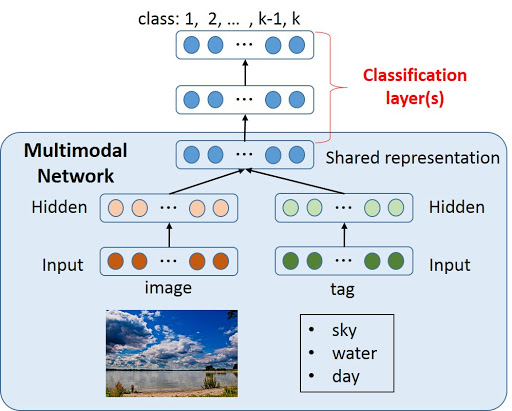
\includegraphics[width=0.70\textwidth]{2/figures/multimodal_network.jpg}
		\caption[Arquitectura de un modelo multimodal de imágenes y texto]{Arquitectura de un modelo multimodal de imágenes y texto.\\
		Fuente: \cite{tec_nishida2015multimodal}. \textit{Multimodal gesture recognition using multi-stream recurrent neural network}.}
		\label{2:fig6}
	\end{center}
\end{figure}

\subsection{Modelo Predictivo}

Son modelos de datos estadísticos utilizados para predecir el comportamiento futuro. En estos, se recopilan datos históricos y actuales, se formula un modelo estadístico, se realizan predicciones y el modelo se valida a medida que se dispone de datos adicionales. Los modelos predictivos analizan el rendimiento pasado para evaluar la probabilidad de que un cliente muestre un comportamiento específico en el futuro. En esta categoría también abarca la búsqueda de patrones ocultos \parencite{gl_gartner2019pm}.

\subsection{Minería de Datos}

La Minería de Datos es un campo de la estadística y las ciencias de la computación referido al proceso que intenta descubrir patrones en grandes volúmenes de conjuntos de datos \parencite{bk_maimon2010datamining}. Normalmente, estos patrones no pueden detectarse mediante la exploración tradicional de datos porque sus relaciones son demasiado complejas o por su gran volumen. Para ello, utiliza métodos de Inteligencia Artificial, Aprendizaje Automático, estadística y sistemas de bases de datos. Estos patrones son recopilados y definidos como un modelo de minería de datos, los cuales pueden aplicarse en los siguientes escenarios \parencite{gl_microsoft2019datamining}:
\begin{itemize}
	\item Previsión.
	\item Riesgo y probabilidad.
	\item Recomendaciones.
	\item Buscar secuencias.
	\item Agrupación.
\end{itemize}

La generación de un modelo de minería de datos forma de un macro-proceso descrita en los siguientes seis pasos representados en la Figura \ref{2:fig7} \parencite{gl_microsoft2019datamining}:
\begin{figure}[h]
	\begin{center}
		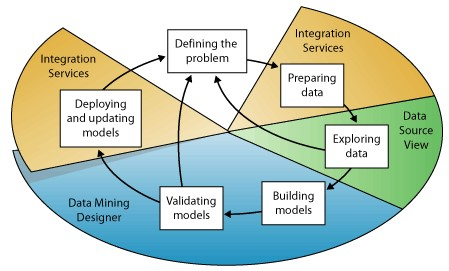
\includegraphics[width=0.7\textwidth]{2/figures/data_mining_steps.jpg}
		\caption[Diagrama de los seis pasos básicos]{Diagrama de los seis pasos básicos.\\
		Fuente: \cite{gl_microsoft2019datamining}. \textit{Conceptos de minería de datos}.}
		\label{2:fig7}
	\end{center}
\end{figure}

\clearpage

\subsection{Metodologías de Minería de Datos}

Dentro de los sistemas de analítica de negocio, Big Data y Minería de Datos, las tres metodologías más usadas se encuentran CRISP-DM, SEMMA y KDD \parencite{tec_braulio2015metodologiasdm}.
\begin{itemize}
	\item \textbf{CRISP-DM} (Cross Industry Standard Process for Data Mining):
	
	Esta metodología presenta seis fases representadas en la Figura \ref{2:fig8} a continuación.
	\begin{figure}[h]
		\begin{center}
			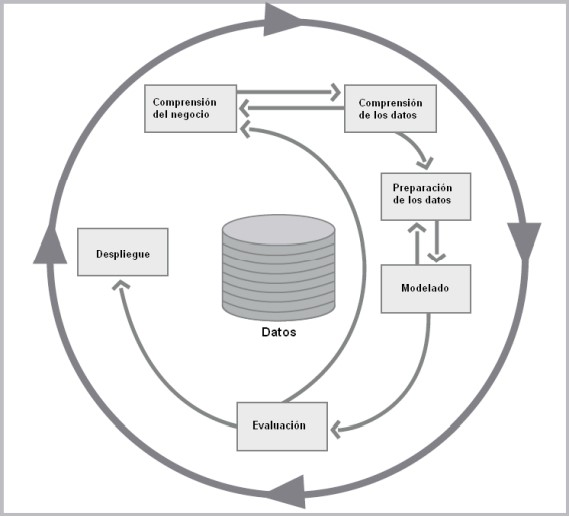
\includegraphics[width=0.65\textwidth]{2/figures/crispdm.jpg}
			\caption[Fases de la metodología CRISP-DM]{Fases de la metodología CRISP-DM.\\
			Fuente: \cite{tec_braulio2015metodologiasdm}. \textit{Customer Analytics: Mejorando la inteligencia del cliente a través de los datos}. (p. 19)}
			\label{2:fig8}
		\end{center}
	\end{figure}
		
	\begin{itemize}
		\item En la comprensión del negocio se determinan los objetivos y requerimientos desde el lado del negocio, así como generar plan del proyecto.
		\item En la comprensión de los datos se logra entender el significado de las variables existentes, así como el entendimiento de los datos desde su recopilación hasta su verificación de calidad.
		\item En la preparación de los datos se prepara el conjunto de datos adecuado que servirán para la construcción del modelo. Por ello, la calidad de los datos es un factor relevante y ello requiere la exclusión de redundancia y valores que no ayuden a establecer buena comprensión y resultados más adelante. A esto se le conoce como limpieza de datos.
		\item En el modelado se aplican técnicas de minería de datos en el conjunto de datos creado en el paso anterior. Para ello, se evalúan entre varias la que mejor performance desempeñe y luego se construye el o los modelos que busquen determinar un objetivo.
		\item En la evaluación se evalúan los posibles modelos del paso anterior a partir del nivel de importancia de acuerdo a las necesidades del negocio y performance que estos cuentan.
		\item El despliegue, finalmente, utiliza el modelo final creado para determinar los objetivos que se buscan cumplir en los requerimientos y ayudar en la toma de decisiones.
	\end{itemize}
	
	\item \textbf{SEMMA} (Sample – Explore – Modify – Model – Assess):
	
	Esta metodología cuenta con cinco fases como se aprecia en la Figura \ref{2:fig9}. A diferencia de la anterior, esta metodología se enfoca más en el modelado.
	\begin{figure}[h]
		\begin{center}
			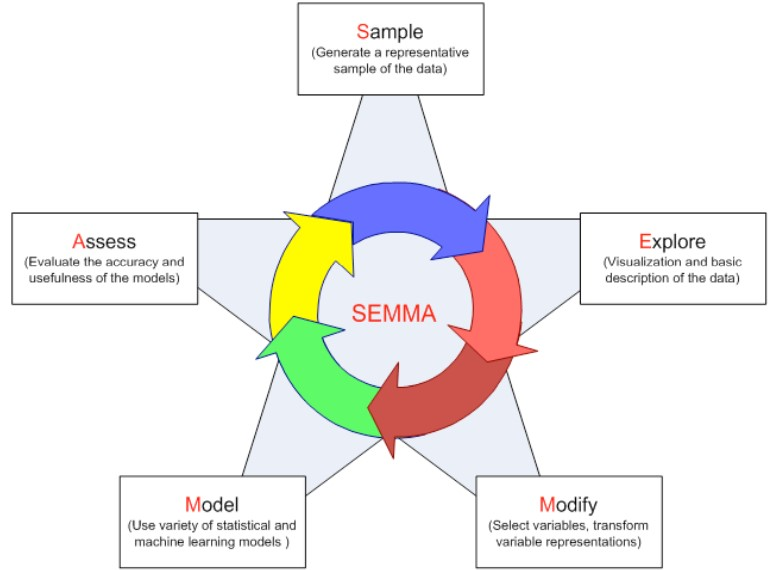
\includegraphics[width=0.70\textwidth]{2/figures/semma.jpg}
			\caption[Fases de la metodología SEMMA]{Fases de la metodología SEMMA.\\
			Fuente: \cite{tec_braulio2015metodologiasdm}. \textit{Customer Analytics: Mejorando la inteligencia del cliente a través de los datos}. (p. 20)}
			\label{2:fig9}
		\end{center}
	\end{figure}
	
	\begin{itemize}
		\item En la Muestra (\textit{Sample}) se crea una muestra significativa.
		\item En la Exploración (\textit{Explore}) se comprenden los datos con el fin de encontrar relaciones entre variables y anomalías.
		\item En la Modificación (\textit{Modify}) se transforman las variables para las necesidades del modelo.
		\item En la Modelización (\textit{Model}) se aplican uno o varios modelos sobre el conjunto de datos para buscar resultados.
		\item En el Asesoramiento (\textit{Assessment}) se evalúan los resultados obtenidos del modelo.
	\end{itemize}
	
	\item \textbf{KDD} (Knowledge Discovery and Data Mining):
	
	Esta metodología se refiere al proceso de encontrar conocimiento alguno en el dato y, a diferencia de sus predecesores, se enfoca en crear aplicaciones de minería de datos. Consta de cinco fases más 1 previa y 1 posterior basadas en la generación de conocimiento como se muestra en la Figura \ref{2:fig10}.
	\begin{figure}[h]
		\begin{center}
			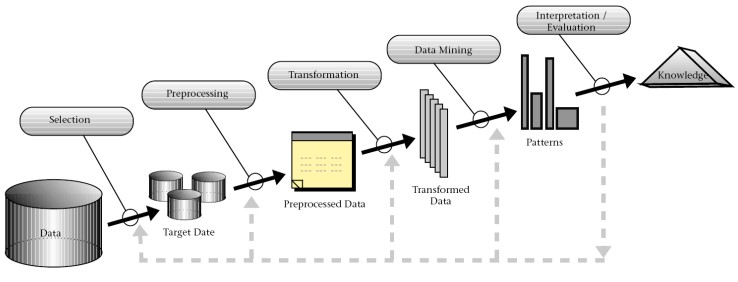
\includegraphics[width=0.80\textwidth]{2/figures/kdd.jpg}
			\caption[Fases de la metodología KDD]{Fases de la metodología KDD.\\
			Fuente: \cite{tec_braulio2015metodologiasdm}. \textit{Customer Analytics: Mejorando la inteligencia del cliente a través de los datos}. (p. 21)}
			\label{2:fig10}
		\end{center}
	\end{figure}
	
	\begin{itemize}
		\item En la fase Pre KDD se comprende el dominio del negocio, así como también se identifican las necesidades del cliente.
		\item En la selección, primero se identifica el conjunto de datos a usar y luego se seleccionan la muestra y las variables para la exploración.
		\item En el pre-procesamiento, se realiza la limpieza de datos y se elimina el ruido, así como los valores atípicos.
		\item En la transformación se implementan métodos de reducción de dimensiones para reducir el número de variables efectivas.
		\item En la Minería de datos, se elige el tipo de tarea de minería de datos (clasificación, regresión, agrupamiento, entre otros) así como el algoritmo, los métodos, los modelos y parámetros apropiados.
		\item En la interpretación y evaluación se analizan los resultados dados.
		\item En la fase Post KDD finalmente se consolida el conocimiento adquirido.
	\end{itemize}

\end{itemize}

Luego de presentar las tres metodologías más usadas, la pregunta dada es ¿cuál de los tres representa la mejor opción para usar?
Las tres metodologías tienen distinto número de pasos, así como distintos enfoques, tal cual se observa en el siguiente resumen de la Tabla \ref{2:table1}.

\begin{table}[htbp]
	\caption[Cuadro comparativo entre características de las tres metodologías]{Cuadro comparativo entre características de las tres metodologías.}
	\label{2:table1}
	\newcommand{\multirot}[1]{\multirow{2}{*}[-8ex]{\rotcell{\rlap{#1}}}}
	%\scriptsize
	\footnotesize
	\centering
	\begin{tabular}{M{3.5cm}M{5cm}M{3.5cm}M{2.5cm}}
		\specialrule{.1em}{.05em}{.05em}
		Modelo de Procesos de Minería de Datos &
		KDD &
		CRISP-DM & 
		SEMMA
		\\
		\specialrule{.1em}{.05em}{.05em}
		{Número de pasos}
		&9
		&6
		&5                                                        
		\\[5pt]
		\hline
		{\multirow{9}{*}[-8ex]{Nombre de los pasos}}
		&Desarrollo y entendimiento de la aplicación
		&Entendimiento del negocio
		&- \\
		\cline{2-4}
		&Creación de un conjunto de datos de destino
		&\multirow{2}{3.5cm}[-2ex]{\centering Entendimiento de los datos}
		&Muestreo
		\\
		\cline{2-2}\cline{4-4}
		&Limpieza de datos y pre-procesamiento
		&\multicolumn{1}{c}{}
		&Exploración
		\\
		\cline{2-4}
		&Transformación de datos
		&Preparación de los datos
		&Modificación
		\\
		\cline{2-4}
		&Elección de la tarea adecuada de Minería de datos
		&\multirow{3}{*}[-3ex]{Modelamiento}
		&\multirow{3}{*}[-3ex]{Modelo}
		\\
		\cline{2-2}
		&Elección del algoritmo adecuado de Minería de datos
		&\multicolumn{1}{c}{}
		&\multicolumn{1}{c}{}
		\\
		\cline{2-2}
		&Implementación del algoritmo de Minería de datos
		&\multicolumn{1}{c}{}
		&\multicolumn{1}{c}{}
		\\
		\cline{2-4}
		&Interpretación de patrones minados
		&Evaluación
		&Evaluación
		\\
		\cline{2-4}          & Uso de conocimiento descubierto & Despliegue & -
		\\
		\specialrule{.1em}{.05em}{.05em}
	\end{tabular}%
	%\par	%%Salto de linea
	%\bigskip
	\begin{flushleft}	%%Alinear a la izquierda sin justificar
		\small Fuente: \cite{tec_shafique2014dmmodels}. \textit{A Comparative Study of Data Mining Process Models (KDD, CRISP-DM and SEMMA). (p. 221)}
	\end{flushleft}
\end{table}

Sin embargo, la elección depende de los involucrados que finalmente usarán el modelo en el negocio. La mayoría de investigadores siguen la metodología KDD debido a que es más completo y su exactitud. Para aquellos objetivos enfocados más en la compañía como la integración usada por SAS Enterprise Miner con su software se utilizan SEMMA y CRISP-DM. Esta última resulta ser más completa de acuerdo a los estudios.

\clearpage

\subsection{Técnicas de Minería de Datos}

Existe una gran variedad de técnicas para la Minería de Datos. Las más importantes y utilizadas en los antecedentes de la investigación se mencionan a continuación \parencite{gl_microsoft2018datamining}.

\begin{itemize}
	\item \textbf{Redes Neuronales Artificiales} (RNA): Es un sistema de computación que consiste en un número de elementos o nodos simples, pero altamente interconectados, llamados “neuronas”, que se organizan en capas que procesan información utilizando respuestas de estado dinámico a entradas externas \parencite{tec_inzaugarat2018ann}.
	
	Este sistema de programas y estructura de datos se aproxima al funcionamiento del cerebro humano. Una red neuronal implica tener un gran número de procesadores funcionando en paralelo, teniendo cada uno de ellos su propia esfera de conocimiento y acceso a datos en su memoria local. Normalmente, una se alimenta con grandes cantidades de datos y un conjunto dado de reglas acerca de las relaciones. Luego, un programa puede indicar a la red cómo debe comportarse en respuesta a un estímulo externo o si puede iniciar la actividad por sí misma \parencite{tec_banafa2019deeplearning}.
	
	Para entender mejor cómo funciona una red neuronal, hay que describir qué es una neurona. Una neurona es una célula del cerebro cuya función principal es la recogida, procesamiento y emisión de señales eléctricas. Debido a que se piensa que la capacidad de procesamiento de información del cerebro proviene de redes de este tipo de neuronas, los primeros trabajos en Inteligencia Artificial se basaron en crear redes neuronales artificiales para emular este comportamiento, en 1943 con un modelo matemático, mostrado en la Figura \ref{2:fig11}, por los ya mencionados anteriormente McCulloch y Pitts.
	\begin{figure}[h]
		\begin{center}
			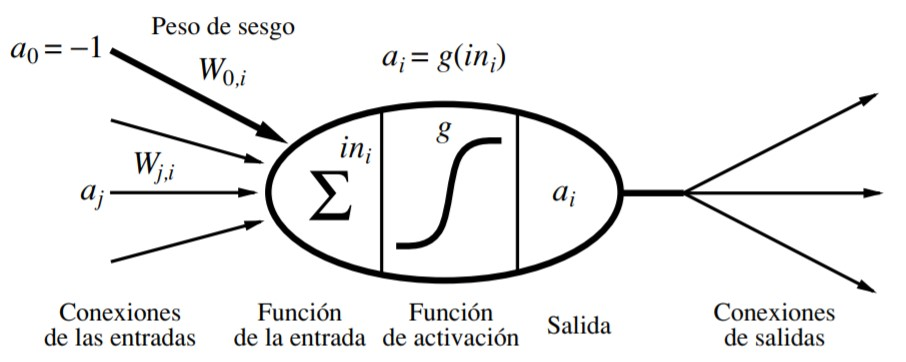
\includegraphics[width=0.75\textwidth]{2/figures/rnn_mcculloch.jpg}
			\caption[Modelo para representar una neurona propuesto por McCulloch y Pitts (1943)]{Modelo para representar una neurona propuesto por McCulloch y Pitts (1943).\\
			Fuente: \cite{bk_russell2004intart}. \textit{Inteligencia Artificial: Un Enfoque Moderno}. (segunda edición). (p. 839)}
			\label{2:fig11}
		\end{center}
	\end{figure}

	Estos y posteriores trabajos potenciaron lo que hoy en día se conoce como el campo de la neurociencia computacional \parencite{bk_russell2004intart}. Años más tarde, en 1958, se desarrolló el concepto del perceptrón por Rosenblatt, el cual tenía la capacidad de aprender y reconocer patrones sencillos, formado por entradas, neurona, función de adaptación (sigmoidal, tangencial, en escalón, etc.) y salida.	La última figura descrita muestra, además de los pesos, funciones de activación tanto para la entrada ($a_j$) como para la salida ($a_i$).
	
	Las redes neuronales están compuestas de nodos (la elipse) conectados a través de conexiones dirigidas (las flechas). Una conexión del nodo $j$ a la unidad $i$ sirve para propagar la activación $a_j$ de $j$ a $i$. Asimismo, cada conexión tiene un peso numérico $W(j,i)$ que determina la fuerza y el signo de la conexión. Para calcular cada nodo $i$, se realiza una suma ponderada de sus entradas (producto entre pesos y nodos de entrada $j$), y se le añade el sesgo (\textit{bias}) $\theta_i$ (aumenta/disminuye el valor de la combinación lineal de las entradas).
	%\begin{equcaption}[!ht]
	\begin{equation}\label{eq:nodo}
	\phantomsection
	in_i=\sum_{j=0}^n W_{j,i}*a_j + \theta_i
	\end{equation}
	\myequations{Fórmula del cálculo del valor de un nodo i}
	%\caption[Fórmula del cálculo del valor de un nodo i]{Fórmula del cálculo del valor de un nodo \textit{i}. Fuente: \cite{bk_russell2004intart}}
	%\end{equcaption}
	
	Posteriormente, se efectúa una función de activación g a esta suma para producir la salida.
	%\begin{equcaption}[!ht]
	\begin{equation}\label{eq:activacion}
	\phantomsection
	a_i = g(in_i) = g \left(\sum_{j=0}^n W_{j,i}*a_j + \theta_i\right)
	\end{equation}
	\myequations{Fórmula de una función de activación g para la salida del nodo}
	%\caption[Fórmula de una función de activación g para la salida del nodo]{Fórmula de una función de activación g para la salida del nodo. Fuente: \cite{bk_russell2004intart}}
	%\end{equcaption}
	
	%\clearpage
	Entonces, aquí se explica los dos objetivos de una función de activación. En primer lugar, se desea que el nodo esté “activo” (cercano a +1) cuando las entradas correctas sean dadas, e “inactiva” (cercano a 0) cuando las entradas erróneas sean proporcionadas. En segundo lugar, la activación tiene que ser no lineal porque, de lo contrario, la red neuronal colapsaría en su totalidad con una función lineal sencilla (Figura \ref{2:fig12}).
	\begin{figure}[h]
		\begin{center}
			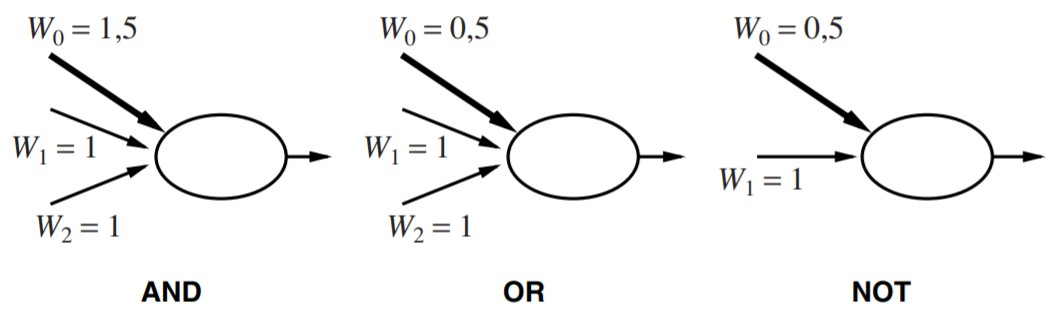
\includegraphics[width=0.75\textwidth]{2/figures/rna_activaciones.jpg}
			\caption[Nodos con funciones de activación umbral en forma de puertas lógicas]{Nodos con funciones de activación umbral en forma de puertas lógicas.\\
			Fuente: \cite{bk_russell2004intart}. \textit{Inteligencia Artificial: Un Enfoque Moderno}. (segunda edición). (p. 840)}
			\label{2:fig12}
		\end{center}
	\end{figure}
	
	Entre las funciones de activación que más destacan son las siguientes:
	\begin{itemize}
		\item \textbf{Función sigmoide o logística}: Toma los valores de entrada que oscilan entre infinito negativo y positivo, y restringe los valores de salida al rango entre 0 y 1. Frecuentemente es usada en Redes Multicapa (MLP) entrenadas con el algoritmo de propagación inversa. Se representa como en la Figura \ref{2:fig13} y su fórmula para calcular su nuevo valor es la Ecuación \ref{eq:sigmoide}:
		%\begin{equcaption}[!ht]
		\begin{equation}\label{eq:sigmoide}
		\phantomsection
		a=Logsig(n)=\frac{1}{1+e^{-n}}
		\end{equation}
		\myequations{Fórmula de la función de activación sigmoide}
		%\caption[Fórmula de la función de activación sigmoide]{Fórmula de la función de activación sigmoide. Fuente: \cite{pr_dorofki2012ann}}
		%\end{equcaption}
		
		\begin{figure}[h]
			\begin{center}
				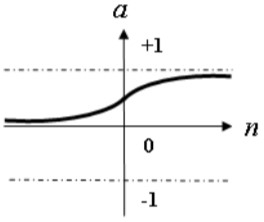
\includegraphics[width=0.3\textwidth]{2/figures/sigmoide.jpg}
				\caption[Función de activación sigmoide]{Función de activación sigmoide.\\
				Fuente: \cite{pr_dorofki2012ann}. \textit{Comparison of Artificial Neural Network Transfer Functions Abilities to Simulate Extreme Runoff Data}. (p. 40)}
				\label{2:fig13}
			\end{center}
		\end{figure}
		
		Un dato curioso de esta función relacionado con la regresión logística es que el nombre de esta última no deriva de una regresión. Por el contrario, se debe a que, al principio de la neurona, se realiza una combinación lineal muy parecida a una regresión lineal y después se aplica la función logística o sigmoide. De ahí el origen del nombre \parencite{gl_iartificial2019reglogistica}.
		\begin{itemize}
			\item \textbf{Regresión Logística}: Como se mencionó antes, es similar a un modelo de regresión lineal, pero está adaptado para modelos en los que la variable dependiente es dicotómica, es decir, presenta solo dos posibles valores. Resulta muy útil para los casos en los que se desea predecir la presencia o ausencia de una característica o resultado según los valores de un conjunto de predictores \parencite{gl_ibm2019reglogistica}. Su función de coste que se optimiza con gradiente descendiente se representa mediante la Ecuación \ref{eq:logistica}:
			%\begin{equcaption}[!ht]
			\begin{equation}\label{eq:logistica}
			\phantomsection
			J(\theta)=\frac{1}{m}\sum_{i=1}^m [-y_i*\log(h_{\theta}(x_{i}))-(1-y_i)*\log(1-h_{\theta}(x_{i}))]
			\end{equation}
			\myequations{Fórmula de función de coste de una regresión logística}
			%\caption[Fórmula de función de coste de una regresión logística]{Fórmula de función de coste de una regresión logística. Fuente: \cite{gl_pardo_reglogcosto}}
			%\end{equcaption}
			
			Donde:
			\begin{conditions}
				h_{\theta}(x_{i})	&	función sigmoide de $\theta^T x$ \\
				\theta	&	vector de longitud theta para j=0,1,2,3...n \\
				x   &  matriz de entradas \\
				y	&  vector de salidas
			\end{conditions}
			
			La primera parte de la ecuación está conformada por el logaritmo de la probabilidad de éxito y la segunda, por la de fracaso.
			
			\item \textbf{Gradiente descendiente}: Es un método de optimización numérica para estimar los mejores coeficientes, fundamental en Deep Learning para entrenar redes neuronales y en muchos casos, para la regresión logística. A través de una función E(W), proporciona el error que comete la red en función del conjunto de pesos sinápticos W. El objetivo del aprendizaje será encontrar la configuración de pesos que corresponda al mínimo global de la función de error o coste \parencite{tec_bertona2005algevol}.
			
			En general, la función de error es una función no lineal, por lo que el algoritmo realiza una búsqueda a través del espacio de parámetros que, se aproxime de forma iterada a un error mínimo de la red para los parámetros adecuados, como se aprecia en la Figura \ref{2:fig14} \parencite{tec_sancho2017descentgrad}.
			\begin{figure}[h]
				\begin{center}
					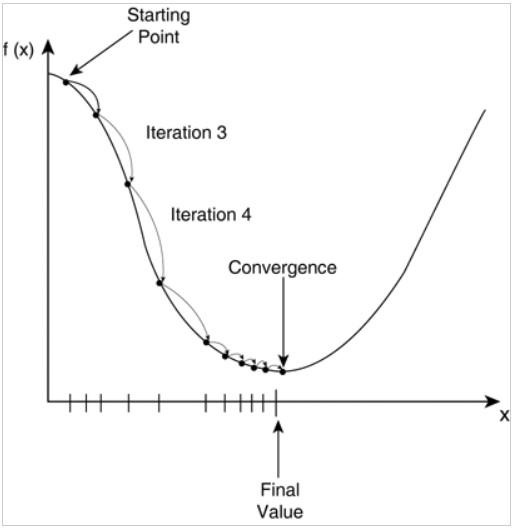
\includegraphics[width=0.40\textwidth]{2/figures/gradiente_descendiente.jpg}
					\caption[Ilustración del algoritmo gradiente descendiente]{Ilustración del algoritmo gradiente descendiente.\\
					Fuente: \cite{tec_sancho2017descentgrad}. \textit{Entrenamiento de Redes Neuronales: mejorando el Gradiente Descendiente}.}
					\label{2:fig14}
				\end{center}
			\end{figure}
			
			El Descenso del Gradiente, como también se le conoce, es el algoritmo de entrenamiento más simple y también el más extendido y conocido. Solo hace uso del vector gradiente, y por ello se dice que es un método de primer orden \parencite{tec_sancho2017descentgrad}. Un gradiente es la generalización de la derivada. Matemática, la derivada de una función mide la rapidez con la que cambia el valor de esta, según varié el valor de su variable independiente. La gradiente se calcula con derivadas parciales, por lo que al actualizar los coeficientes W para un tiempo t, se usa la Ecuación \ref{eq:w_descgrad} \parencite{gl_iartificial2019descentgrad}:
			%\begin{equcaption}[!ht]
			\begin{equation}\label{eq:w_descgrad}
			\phantomsection
			W_{(t+1)}=W_{(t)}-\alpha \left(\frac{\partial MSE}{\partial W} \right)
			\end{equation}
			\myequations{Actualización de pesos W mediante gradiente descendiente}
			%\caption[Actualización de pesos W mediante gradiente descendiente]{Actualización de pesos W mediante gradiente descendiente. Fuente: \cite{gl_iartificial2019descentgrad}}
			%\end{equcaption}
		
			Donde: $\alpha$ = ratio de aprendizaje
			
			Este ratio controla el tamaño de la actualización. Si este es demasiado grande, será más difícil encontrar los coeficientes que minimicen la función de coste o error; la actualización de W es proporcional al gradiente; y se usa la resta para ir en dirección opuesta al gradiente como en la Figura \ref{2:fig15}.
			\begin{figure}[h]
				\begin{center}
					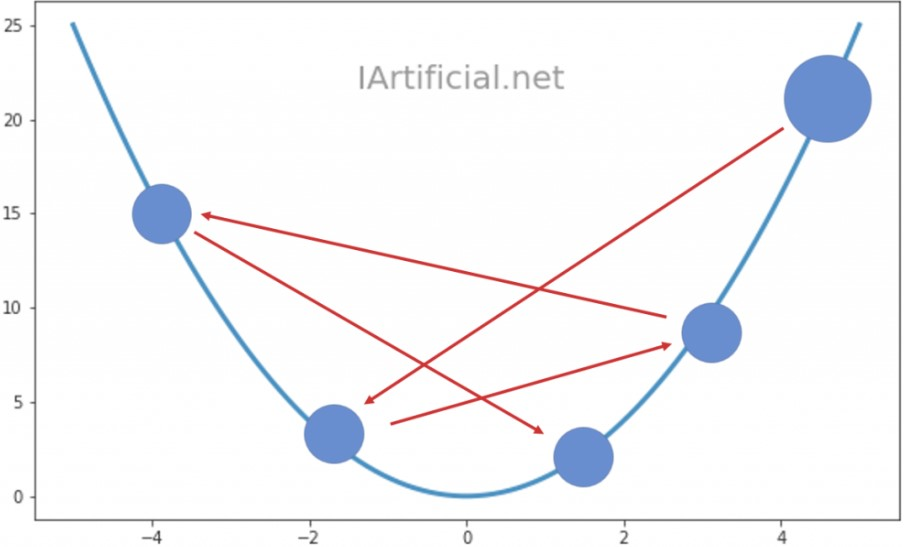
\includegraphics[width=0.47\textwidth]{2/figures/pesos_graddescen.jpg}
					\caption[Actualización de pesos W con el algoritmo]{Actualización de pesos W con el algoritmo.\\
					Fuente: \cite{gl_iartificial2019descentgrad}. \textit{Método del Gradiente Descendiente}.}
					\label{2:fig15}
				\end{center}
			\end{figure}
			
			\item \textbf{Propagación hacia atrás}: También conocido en inglés como \textit{Backpropagation}, es un método que consta de dos fases: en la primera se aplica un patrón, el cual se propaga por las distintas capas que componen la red hasta producir la salida de la misma. Luego, esta se compara con la salida deseada y se calcula el error cometido por cada neurona de salida. Estos errores se transmiten hacia atrás, partiendo de la capa de salida, hacia todas las neuronas de las capas intermedias [Fritsch, 1996] \parencite{tec_bertona2005algevol}. La actualización iterativa de los pesos que el algoritmo propone es mediante la Ecuación \ref{eq:backpropagation}:
			%\begin{equcaption}[!ht]
			\begin{equation}\label{eq:backpropagation}
			\phantomsection
			W_{ji}(t+1)=W_{ji}(t)+[\alpha \delta_{pj} y_{pj} + \beta \Delta W_{ji}(t)]
			\end{equation}
			\myequations{Fórmula del algoritmo de propagación hacia atrás}
			%\caption[Fórmula del algoritmo de propagación hacia atrás]{Fórmula del algoritmo de propagación hacia atrás. Fuente: \cite{tec_bertona2005algevol}}
			%\end{equcaption}
			
			\begin{equation*}
			%\phantomsection
			\text{siendo} \quad \delta_{pj} =
			\left\{
			\begin{aligned}
				(d_{pj}-y_{pj})f'_j(h_j) \quad\text{si j es una neurona de salida}\\
				\left(\sum_{k} \delta_{pk} W_{kj}\right)f'_j(h_j) \quad\text{si j es una neurona oculta}
			\end{aligned}
			\right.
			\end{equation*}
			
			\begin{figure}[h]
				\begin{center}
					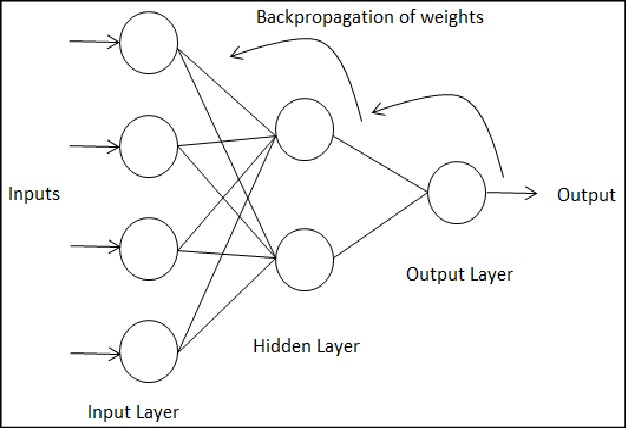
\includegraphics[width=0.5\textwidth]{2/figures/backpropagation.jpg}
					\caption[Capa oculta simple MLP con propagación hacia atrás]{Capa oculta simple MLP con propagación hacia atrás.\\
					Fuente: \cite{gl_iartificial2019descentgrad}. \textit{Método del Gradiente Descendiente}.}
					\label{2:fig16}
				\end{center}
			\end{figure}
			
			Para entender mejor la teoría y la fórmula de actualización de pesos, se seguirá el siguiente ejemplo del conjunto de redes de la Figura \ref{2:fig17}.
			
			\begin{figure}[h]
				\begin{center}
					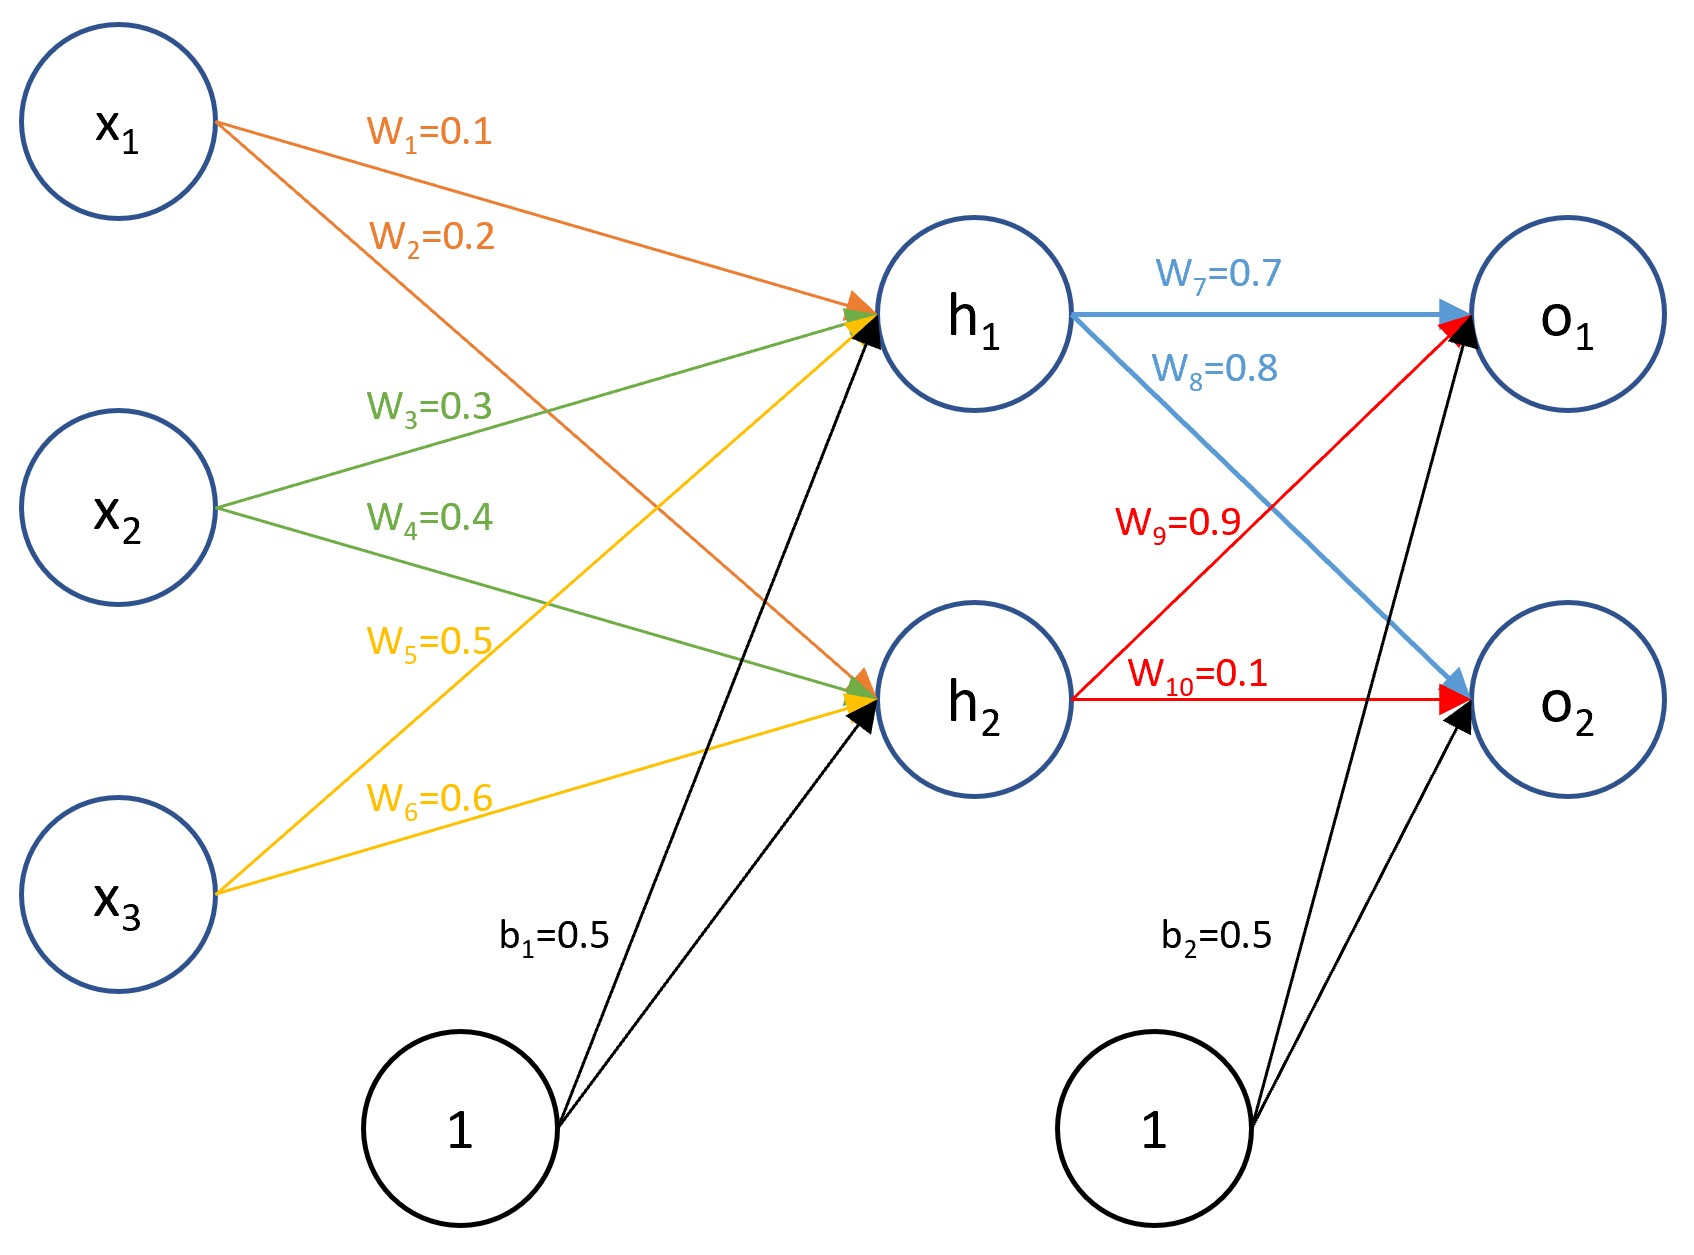
\includegraphics[width=0.58\textwidth]{2/figures/rna_pesos.jpg}
					\caption[Redes neuronales de ejemplo]{Redes neuronales de ejemplo.\\
					Fuente: \cite{gl_ansrw2019backpropagation}. \textit{Backpropagation Example With Numbers Step by Step}.}
					\label{2:fig17}
				\end{center}
			\end{figure}
			
			Se tiene una red neuronal con tres nodos de entradas ($x_1$=1, $x_2$=4 y $x_3$=5) con dos pesos respectivos cada una ($W_1$=0.1 y $W_2$=0.2 para $x_1$; $W_3$=0.3 y $W_4$=0.4 para $x_2$; $W_5$=0.5 y $W_6$=0.6 para $x_3$), dos capas ocultas ($h_1$ y $h_2$) con dos peso cada una ($W_7$=0.7 y $W_8$=0.8 para $h_1$; $W_9$=0.9 y $W_10$=0.1 para $h_2$) y dos nodos de salida ($O_1$ y $O_2$).
			
			El proceso normal para calcular el valor del nodo final se da, tanto con los nodos de entrada y los de capa oculta, mediante la sumatoria de producto de cada peso con su valor, es decir, mediante la fórmula de las RNA $in_i=\sum_{j=0}^n W_{j,i}*a_j+b_{j,i}$, al mismo tiempo que devuelve un valor del error cometido. Este último se calcula mediante la Ecuación \ref{eq:rnaerror}:
			%\begin{equcaption}[!ht]
			\begin{equation}\label{eq:rnaerror}
			\phantomsection
			E_k=(T_k-O_k)*O_k*(1-O_k)
			\end{equation}
			\myequations{Cálculo del error cometido en una red neuronal}
			%\caption[Cálculo del error cometido en una red neuronal]{Cálculo del error cometido en una red neuronal. Fuente: \cite{tec_viera2013backpropexplain}}
			%\end{equcaption}
			
			Donde:
			\begin{conditions}
				T_k	&	salida correcta de cada nodo de salida \\
				O_k	&	salida actual que cada nodo genera
			\end{conditions}
			
			Con estos errores, se retrocede hacia la capa oculta y se procede a calcular los nuevos pesos para sus nodos. Esto se realiza mediante la Ecuación \ref{eq:updateweightsrna}:
			%\begin{equcaption}[!ht]
			\begin{equation}\label{eq:updateweightsrna}
			\phantomsection
			W_{jk}=W_{jk}+L*E_k*O_j
			\end{equation}
			\myequations{Actualización de pesos mediante propagación hacia atrás}
			%\caption[Actualización de pesos mediante propagación hacia atrás]{Actualización de pesos mediante propagación hacia atrás. Fuente: \cite{tec_viera2013backpropexplain}}
			%\end{equcaption}
			
			Donde:
			\begin{conditions}
				W_{jk}	&	peso a actualizar para cada nodo de la capa oculta ($W_7$, $W_8$, $W_9$ y $W_{10}$) \\
				L	&	porcentaje de aprendizaje \\
				O_j	&	valor de los nodos que entrarán a las salidas
			\end{conditions}
			
			Estos nuevos pesos permitirán redefinir los errores de ambos nodos, con una pequeña diferencia en su cálculo (Ecuación \ref{eq:errornodorna}):
			%\begin{equcaption}[!ht]
			\begin{equation}\label{eq:errornodorna}
			\phantomsection
			E_{j}=O_{j}*(1-O_{j})*\sum E_{k}*W_{jk}
			\end{equation}
			\myequations{Cálculo de errores de nodos usando pesos actualizados}
			%\caption[Cálculo de errores de nodos usando pesos actualizados]{Cálculo de errores de nodos usando pesos actualizados. Fuente: \cite{tec_viera2013backpropexplain}}
			%\end{equcaption}
			
			El error de cada nodo de la capa oculta se obtiene multiplicando su valor por su complemento por la sumatoria del producto de sus pesos y los errores de los nodos de salida. Por ejemplo, para h1 sería 
			$E_{h1}=h_1*(1-h_1)*(0.7*O_1+0.8*O_2)$.
			
			Finalmente, se retrocede hacia los nodos de entrada y se repite el mismo proceso para la actualización de sus pesos y errores.
		\end{itemize}
	\item \textbf{Función tangente hiperbólica}: Esta función está relacionada con una sigmoide bipolar. Sin embargo, sus salidas estarán en el rango de -1 y +1. Para redes neuronales, donde la velocidad es más importante que la forma de la función misma, es recomendable usar esta. Se representa como en la Figura \ref{2:fig18} y su fórmula para calcular su nuevo valor es la Ecuación \ref{eq:tansig}:
	\begin{figure}[!ht]
		\begin{center}
			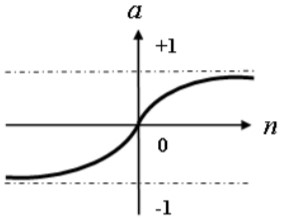
\includegraphics[width=0.30\textwidth]{2/figures/hiperbolica.jpg}
			\caption[Función de activación tangente hiperbólica]{Función de activación tangente hiperbólica.\\
			Fuente: \cite{pr_dorofki2012ann}. \textit{Comparison of Artificial Neural Network Transfer Functions Abilities to Simulate Extreme Runoff Data}. (p. 40)}
			\label{2:fig18}
		\end{center}
	\end{figure}
	
	%\begin{equcaption}[!ht]
	\begin{equation}\label{eq:tansig}
	\phantomsection
	a=Tansig(n)=\frac{2}{1+e^{-2n}}-1
	\end{equation}
	\myequations{Fórmula de la función de activación tangente hiperbólica}
	%\caption[Fórmula de la función de activación tangente hiperbólica]{Fórmula de la función de activación tangente hiperbólica. Fuente: \cite{pr_dorofki2012ann}}
	%\end{equcaption}

	\item \textbf{Función puramente lineal (purelin)}: Se caracteriza porque su salida es igual a su entrada debido a su linealidad. Normalmente se usa para obtener los mismos valores de entrada. Se representa en la Figura \ref{2:fig19} y se calcula mediante la Ecuación \ref{eq:purelin}:
	
	\begin{figure}[h]
		\begin{center}
			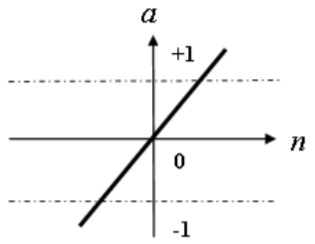
\includegraphics[width=0.30\textwidth]{2/figures/purelin.jpg}
			\caption[Función de activación puramente lineal]{Función de activación puramente lineal.\\
			Fuente: \cite{pr_dorofki2012ann}. \textit{Comparison of Artificial Neural Network Transfer Functions Abilities to Simulate Extreme Runoff Data}. (p. 40)}
			\label{2:fig19}
		\end{center}
	\end{figure}

	%\begin{equcaption}[!ht]
	\begin{equation}\label{eq:purelin}
	\phantomsection
	a=n
	\end{equation}
	\myequations{Fórmula de la función de activación puramente lineal}
	%\caption[Fórmula de la función de activación puramente lineal]{Fórmula de la función de activación puramente lineal. Fuente: \cite{pr_dorofki2012ann}}
	%\end{equcaption}
	
	\item \textbf{Función Unidad Lineal Rectificada (ReLU)}: Se caracteriza por conservar los valores positivos y convertir los negativos de entrada en 0, con la finalidad de no considerarlos en la siguiente capa de convolución \parencite{gl_bigdata2019bigdata}. Si bien tiene un buen desempeño en redes convolucionales y es muy usada para procesar imágenes, al no estar acotada pueden morirse demasiadas neuronas \parencite{gl_calvo2018activrna}. Se representa en la Figura \ref{2:fig20} y se calcula mediante la Ecuación \ref{eq:relu}:
	\begin{figure}[h]
		\begin{center}
			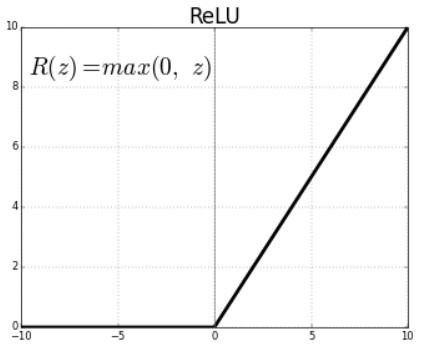
\includegraphics[width=0.30\textwidth]{2/figures/relu.jpg}
			\caption[Función de activación ReLU]{Función de activación ReLU.\\
			Fuente: \cite{gl_mlfa2019redesneuronales}. \textit{Redes Neuronales}.}
			\label{2:fig20}
		\end{center}
	\end{figure}
	
	%\begin{equcaption}[!ht]
	\begin{equation}\label{eq:relu}
	\phantomsection
	f(x) = \max (0,x) =
	\left\{
	\begin{aligned}
	0 \quad \text{para} \quad x < 0\\
	x \quad \text{para} \quad x \geq 0
	\end{aligned}
	\right.
	\end{equation}
	\myequations{Fórmula de la función de activación ReLU}
	%\caption[Fórmula de la función de activación ReLU]{Fórmula de la función de activación ReLU. Fuente: \cite{gl_calvo2018activrna}}
	%\end{equcaption}
	
	\end{itemize}
	
	Además de existir distintas funciones de activación, las redes neuronales artificiales se clasifican según la topología de red, siendo algunas de las más importantes \parencite{gl_calvo2017clasifrna}.
	
	\begin{itemize}
		\item \textbf{Red Neuronal Monocapa – Perceptrón simple}: Es la red neuronal más simple ya que está compuesta solamente de una capa de neuronas que componen varios nodos de entrada para proyectar una capa de neuronas de salida, como se aprecia en la Figura \ref{2:fig21}. Esta última capa se calcula usando la misma Ecuación 4 que implica la suma de productos de cada uno de los pesos de los nodos de entrada con sus instancias, añadiéndole finalmente el sesgo, aquel que controla la predisposición de la neurona a disparar un 1 o 0 independientemente de los pesos, para que el valor resultante se le aplique la función de activación que ayudarán a modelar funciones curvas o no triviales \parencite{gl_mlfa2019redesneuronales}.
		\begin{figure}[h]
			\begin{center}
				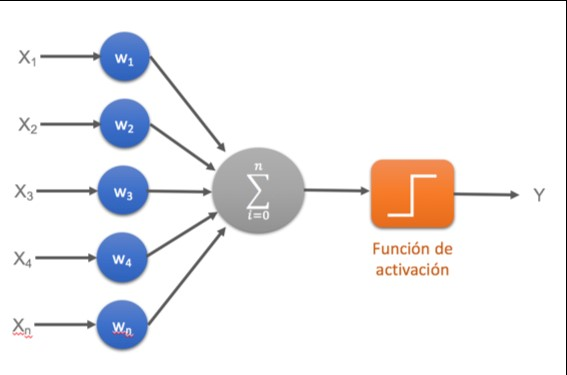
\includegraphics[width=0.55\textwidth]{2/figures/perceptron_simple.jpg}
				\caption[Ejemplo de perceptrón simple]{Ejemplo de perceptrón simple.\\
				Fuente: \cite{gl_calvo2017clasifrna}. \textit{Clasificación de redes neuronales artificiales}.}
				\label{2:fig21}
			\end{center}
		\end{figure}
		
		\newpage
		\item \textbf{Red Neuronal Multicapa – Perceptrón multicapa}: Con arquitectura similar al perceptrón simple, con el añadido de contener capas intermedias entre la capa de neuronas de entrada y la de salida, conocidas como capas ocultas, como en el ejemplo de la Figura \ref{2:fig22}.
		\begin{figure}[h]
			\begin{center}
				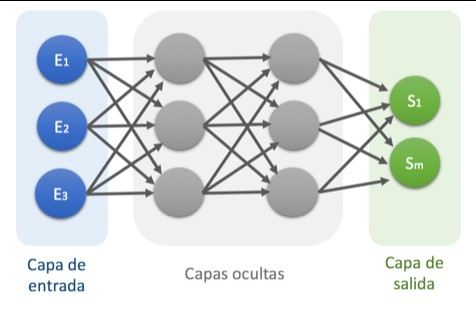
\includegraphics[width=0.55\textwidth]{2/figures/perceptron_multicapa.jpg}
				\caption[Ejemplo de perceptrón multicapa]{Ejemplo de perceptrón multicapa.\\
				Fuente: \cite{gl_calvo2017clasifrna}. \textit{Clasificación de redes neuronales artificiales}.}
				\label{2:fig22}
			\end{center}
		\end{figure}
		
		\item \textbf{Redes Neuronales Convolucionales (CNN)}: También conocidas por su nombre en inglés \textit{Convolutional Neural Networks}, se diferencia del perceptrón multicapa en que cada neurona no necesita estar unida con todas las que le siguen, sino más bien solo con un subgrupo de estas con el fin de reducir la cantidad de neuronas necesarias para su funcionamiento, como se observa en la Figura \ref{2:fig23} \parencite{gl_calvo2017clasifrna}.
		\begin{figure}[h]
			\begin{center}
				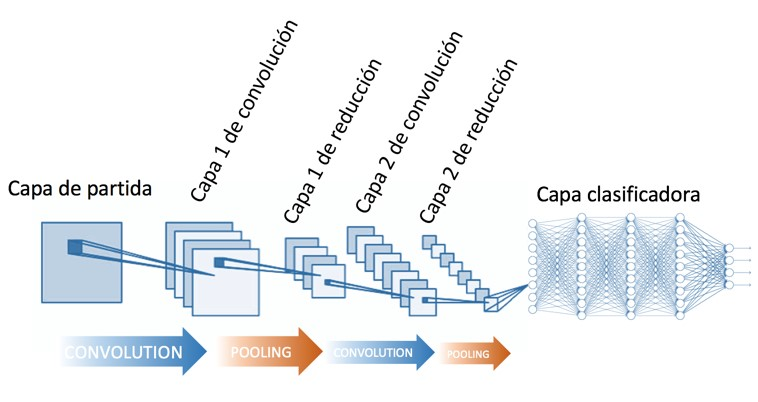
\includegraphics[width=0.50\textwidth]{2/figures/cnn.jpg}
				\caption[Ejemplo de red neuronal convolucional]{Ejemplo de red neuronal convolucional.\\
				Fuente: \cite{gl_calvo2017clasifrna}. \textit{Clasificación de redes neuronales artificiales}.}
				\label{2:fig23}
			\end{center}
		\end{figure}
		
		Hoy en día, las redes neuronales convolucionales tienen múltiples usos desde que la idea fue concebida. Algunos de los problemas en las que pueden ser usados son de clasificación de objetos, recuperación de imágenes, detección y segmentación de objetos, distorsión y filtros de imágenes, por citar los ejemplos más comunes. El modelo de CNN más conocido es “AlexNet” (2012) por ser uno de los pioneros en clasificar imágenes \parencite{tec_li2019cnn}.
		
		En la Figura \ref{2:fig24}, se ilustran redes neuronales que dieron origen a la CNN. La primera imagen representa el Neocognitron introducido por Fukushima en 1980 como modelo de red neuronal para el mecanismo de reconocimiento de patrón visual sin la enseñanza de un “profesor”, mismo que en el año 1998 sería mejorado por LeCun, Bottou, Bengio y Haffner al agregar un método de aprendizaje de gradiente aplicado al reconocimiento de documento basado en la propagación hacia atrás y representado en la segunda imagen \parencite{tec_li2019cnn}.
		
		\begin{figure}[!ht]
			\centering
			\small
			\begin{subfigure}{.5\textwidth}
				\centering
				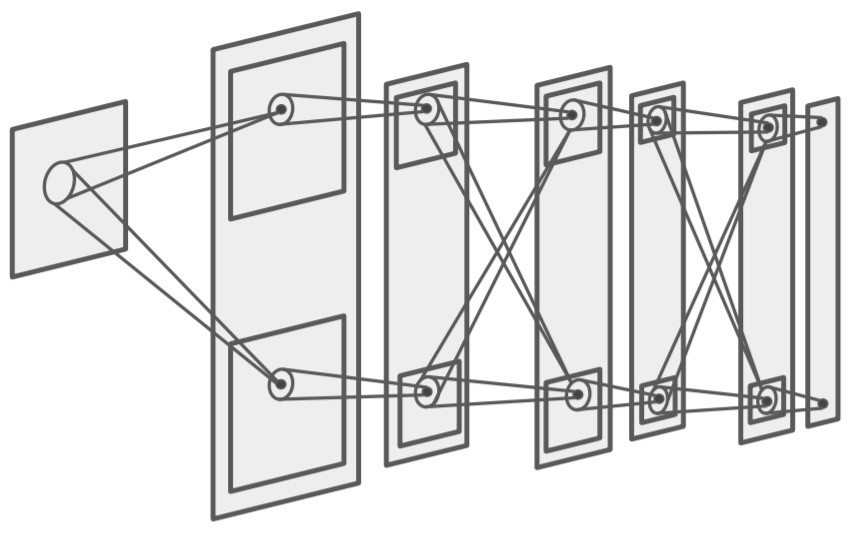
\includegraphics[width=0.62\textwidth]{2/figures/neocognitron.jpg}
				\caption{Modelo Neocognitron de Fukushima (1980)}
			\end{subfigure}%
			\begin{subfigure}{.5\textwidth}
				\centering
				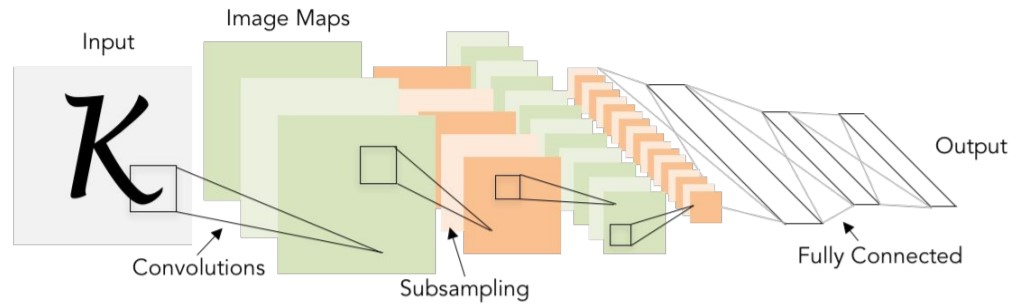
\includegraphics[width=1.22\textwidth]{2/figures/lenet5.jpg}
				\caption{Modelo LeNet-5 de LeCun (1998)}
			\end{subfigure}
			\caption[Modelos de redes neuronales que inspiraron a la CNN]{Modelos de redes neuronales que inspiraron a la CNN.\\
				Fuente: \cite{tec_li2019cnn}. \textit{Convolutional Neural Networks}. (pp. 6, 15)}
			\label{2:fig24}
		\end{figure}
		
		Estos modelos se inspiraron en el estudio de la información visual en la corteza donde se ubican hasta 5 áreas. La primera, V1, contiene la información visual donde sus neuronas se ocupan de características visuales de bajo nivel, alimentando así a otras áreas adyacentes. Cada una de ellas se encarga de aspectos más específicos y detallados de la información obtenida. La idea de su implementación es la de solucionar el problema que surgen al escalar imágenes de mucha definición por las redes neuronales ordinarias. Por ello, este tipo de redes trabajan modelando de forma consecutiva piezas pequeñas de información para luego combinarlas en sus capas más profundas \parencite{tec_lopez2016cnnTF}.
		
		Su nombre deriva del concepto convolución. La convolución es un término en las matemáticas usado como operador matemático que convierte dos funciones f y g en una tercera función en donde la primera se superpone a una versión invertida y trasladada de la segunda, así como para denotar la distribución de la función de probabilidad de la suma de dos variables independientes aleatorias. Esta se da por la Ecuación \ref{eq:convolution} \parencite{tec_figueroa_convolucion}:
		
		%\begin{equcaption}[!ht]
		\begin{equation}\label{eq:convolution}
		\phantomsection
		(f*g)(t)=\int_0^t f(t-\tau)g(\tau)\mathrm{d}\tau
		\end{equation}
		\myequations{Fórmula matemática de la convolución}
		%\caption[Fórmula matemática de la convolución]{Fórmula matemática de la convolución. Fuente: \cite{tec_figueroa_convolucion}}
		%\end{equcaption}
		
		Donde el rango puede variar entre un conjunto finito (como en la fórmula desde 0 hasta un valor t) o uno infinito.
		
		La estructura de las Redes Neuronales Convolucionales se constituye en tres tipos de capas \parencite{tec_lopez2016cnnTF}.
		\begin{itemize}
			\item \textbf{Capa convolucional (\textit{Convolutional Layer})}: Es la capa que hace distinta a esta red de otros tipos de redes neuronales artificiales. Se aplica la operación de la convolución, que recibe como entrada (\textit{input} en inglés) a la imagen para luego aplicarle un filtro (\textit{kernel} en inglés), devolviendo un mapa de las características de la imagen original, logrando así reducir el tamaño de los parámetros, como se observa en la Figura \ref{2:fig25}.
			\begin{figure}[h]
				\begin{center}
					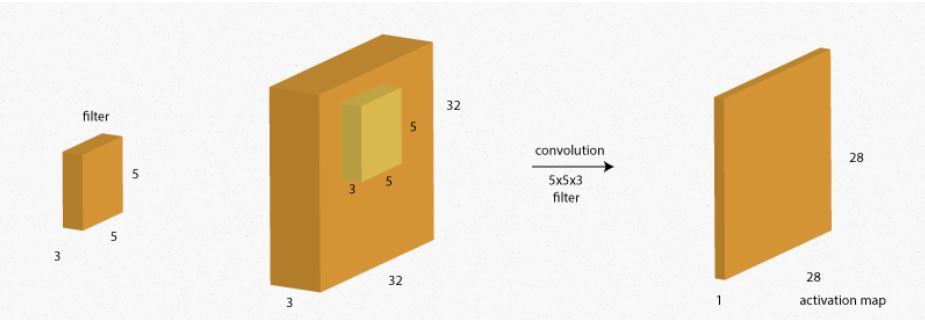
\includegraphics[width=0.80\textwidth]{2/figures/convolucion.jpg}
					\caption[Ejecución de la convolución en una entrada]{Ejecución de la convolución en una entrada.\\
					Fuente: \cite{tec_lopez2016cnnTF}. \textit{Redes neuronales convolucionales con TensorFlow}.}
					\label{2:fig25}
				\end{center}
			\end{figure}
			
			Por ejemplo, en la anterior figura se tiene una imagen de entrada con dimensiones de 32 de alto, 32 de ancho y 3 de profundidad (32x32x3). A ella se le aplica un filtro de dimensiones (5x5x3) que recorrerá toda la imagen para extraer características de cada pixel. Tanto la profundidad de la entrada como del filtro siempre son iguales. El resultado de tomar un producto escalar entre el filtro y un pequeño fragmento de 5x5x3 de la imagen es un número, generando así un mapa de activación de nuevas dimensiones (28x28x1). Por cada n filtros aplicados a la entrada se generan n de estos mapas. Al final, la cantidad de mapas de activación determinará una nueva imagen de n de profundidad, como en la Figura \ref{2:fig26}.
			\begin{figure}[h]
				\begin{center}
					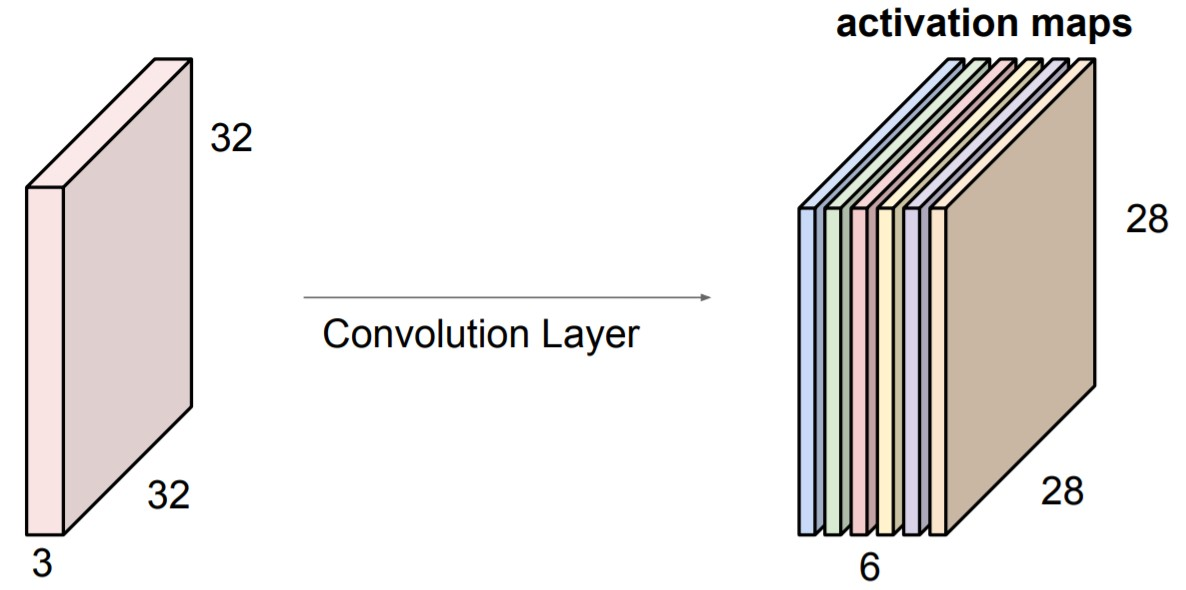
\includegraphics[width=0.70\textwidth]{2/figures/filtros_cnn.jpg}
					\caption[Generación de una nueva imagen a partir de filtros]{Generación de una nueva imagen a partir de filtros.\\
					Fuente: \cite{tec_li2019cnn}. \textit{Convolutional Neural Networks}. (p. 36)}
					\label{2:fig26}
				\end{center}
			\end{figure}
			
			Asimismo, cada vez que se aplica una convolución a una imagen, se aplicará una función de activación como en la secuencia de la Figura \ref{2:fig27}.
			\begin{figure}[h]
				\begin{center}
					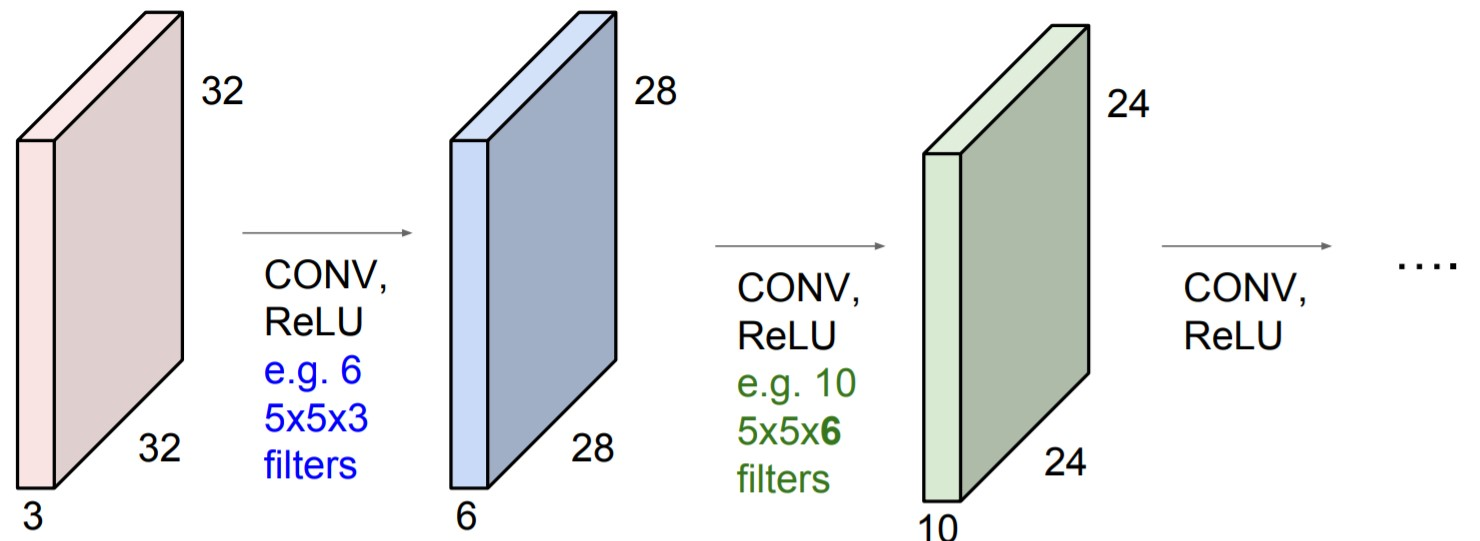
\includegraphics[width=0.70\textwidth]{2/figures/capas_cnn.jpg}
					\caption[Secuencia de varias capas convolucionales]{Secuencia de varias capas convolucionales.\\
					Fuente: \cite{tec_li2019cnn}. \textit{Convolutional Neural Networks}. (p. 38)}
					\label{2:fig27}
				\end{center}
			\end{figure}
			
			A nivel visual, en la Figura \ref{2:fig28} se aprecia un ejemplo de los resultados de aplicar varias convoluciones a una imagen.
			\begin{figure}[h]
				\begin{center}
					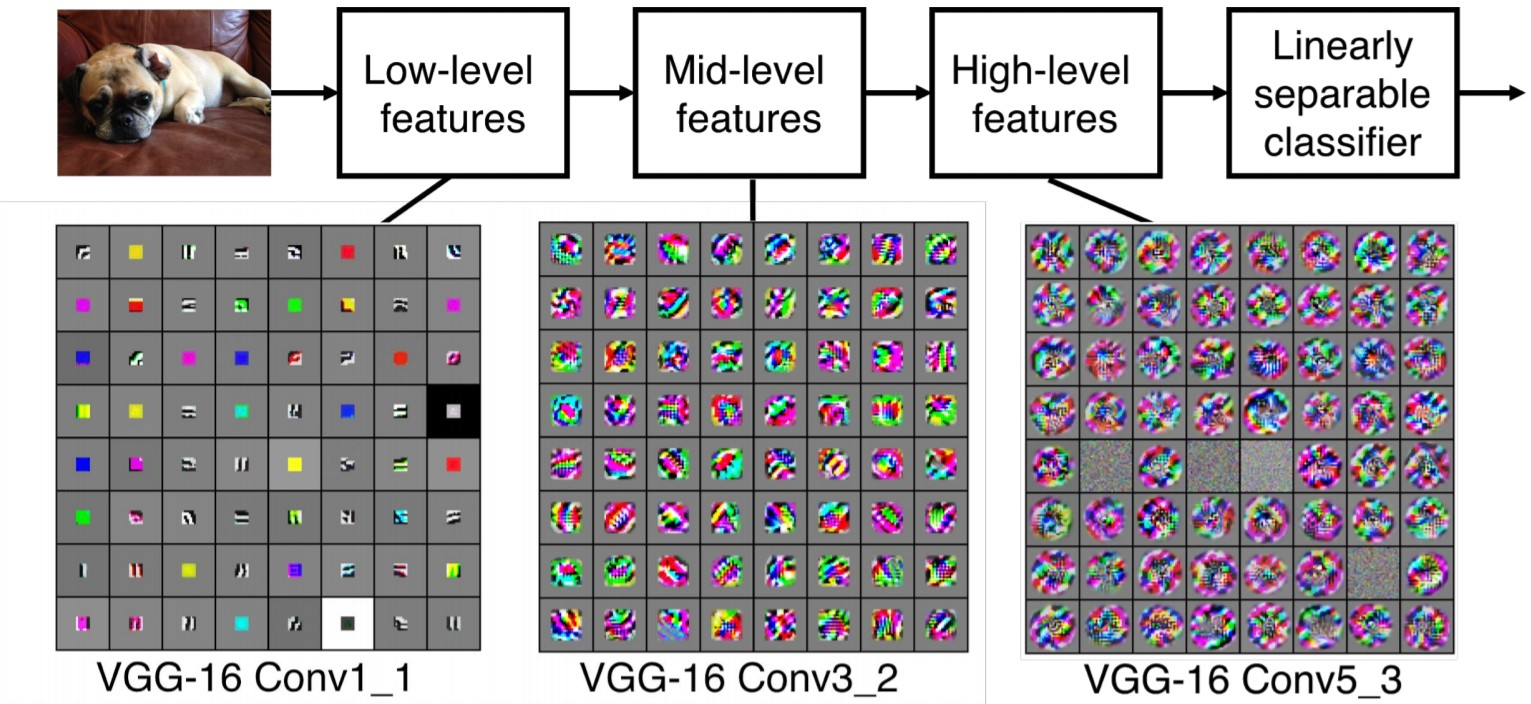
\includegraphics[width=0.70\textwidth]{2/figures/features_cnn.jpg}
					\caption[Extracción de características a partir de convoluciones]{Extracción de características a partir de convoluciones.\\
					Fuente: \cite{tec_li2019cnn}. \textit{Convolutional Neural Networks}. (p. 39)}
					\label{2:fig28}
				\end{center}
			\end{figure}
			
			Finalmente, se calcula el volumen de la dimensión de la salida de la Figura \ref{2:fig29} mediante la Ecuación \ref{eq:mapaact}:
			\begin{itemize}
				\item Se tiene una entrada de dimensiones $(h * w * d)$.
				\item Se tiene un filtro de dimensiones $(f_h * f_w * d)$.
			\end{itemize}
			
			\begin{figure}[h]
				\begin{center}
					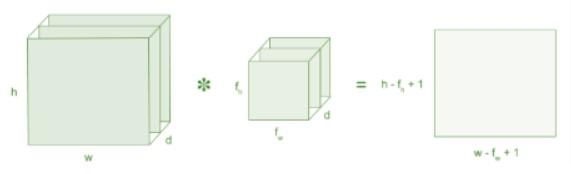
\includegraphics[width=0.75\textwidth]{2/figures/matriz_cnn.jpg}
					\caption[Ejemplo de matriz de imagen de entrada y un filtro]{Ejemplo de matriz de imagen de entrada y un filtro.\\
					Fuente: \cite{tec_prabhu2018cnn}. \textit{Understanding of Convolutional Neural Network (CNN) — Deep Learning}.}
					\label{2:fig29}
				\end{center}
			\end{figure}
			
			%\begin{equcaption}[!ht]
			\begin{equation}\label{eq:mapaact}
			\phantomsection
			Volumen=(h-f_h+1)*(w-f_w+1)*1
			\end{equation}
			\myequations{Cálculo del volumen del mapa de activación}
			%\caption[Cálculo del volumen del mapa de activación]{Cálculo del volumen del mapa de activación. Fuente: \cite{tec_prabhu2018cnn}}
			%\end{equcaption}
			
			\item \textbf{Capa de reducción (\textit{Pooling Layer})}: Esta capa le sucede a la capa convolucional (luego de aplicar la función de activación). Sirve principalmente para reducir las dimensiones espaciales del volumen de la entrada (alto x ancho) para la siguiente capa convolucional. Sin embargo, no afecta la profundidad de la misma. Esta operación que realiza se le conoce también como “reducción de muestreo” debido a que, si bien logra reducir las dimensiones para procesar mejor en la siguiente capa, también conlleva perder información. Por el contrario de lo que se piensa, además de reducir la sobrecarga del cálculo para las siguientes capas, el modelo se beneficia también disminuyendo el sobreajuste.
			
			Para determinar las dimensiones de la nueva imagen generada (siempre que sea cuadrada como en la Figura \ref{2:fig30}) con esta capa, se aplica la Ecuación \ref{eq:outputconv}:
			\begin{figure}[htbp]
				\begin{center}
					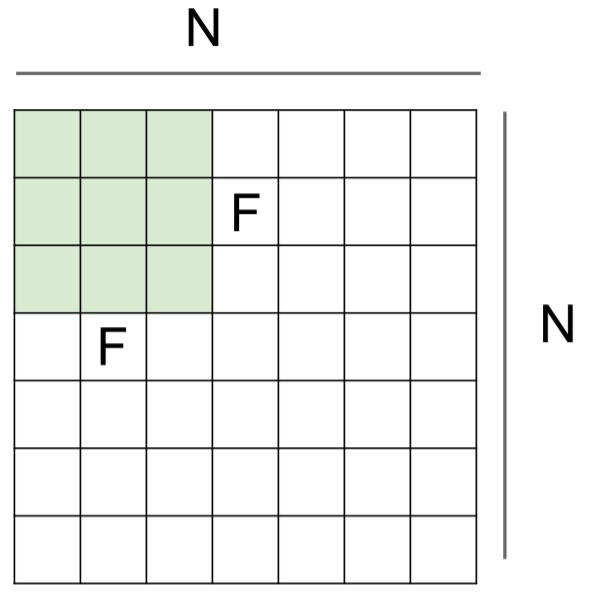
\includegraphics[width=0.25\textwidth]{2/figures/input_filter_cnn.jpg}
					\caption[Dimensiones de una entrada y un filtro]{Dimensiones de una entrada y un filtro.\\
					Fuente: \cite{tec_li2019cnn}. \textit{Convolutional Neural Networks}. (p. 54)}
					\label{2:fig30}
				\end{center}
			\end{figure}
		
			%\begin{equcaption}[!ht]
			\begin{equation}\label{eq:outputconv}
			\phantomsection
			Salida=\frac{N-F}{S}+1
			\end{equation}
			\myequations{Cálculo del tamaño de la imagen reducida}
			%\caption[Cálculo del tamaño de la imagen reducida]{Cálculo del tamaño de la imagen reducida. Fuente: \cite{tec_li2019cnn}}
			%\end{equcaption}
		
			Donde:
			\begin{conditions}
				N   &  tamaño del lado de la imagen de entrada \\
				F   &  tamaño del lado del filtro \\   
				S	&  número de desplazamiento de pixeles sobre la matriz de entrada
			\end{conditions}
			
			Si el paso es 1, los filtros se mueven a 1 pixel por vez, cuando si es 2, se mueven a 2 píxeles (como en la Figura \ref{2:fig31}) y así sucesivamente \parencite{tec_prabhu2018cnn}.
			\begin{figure}[htbp]
				\begin{center}
					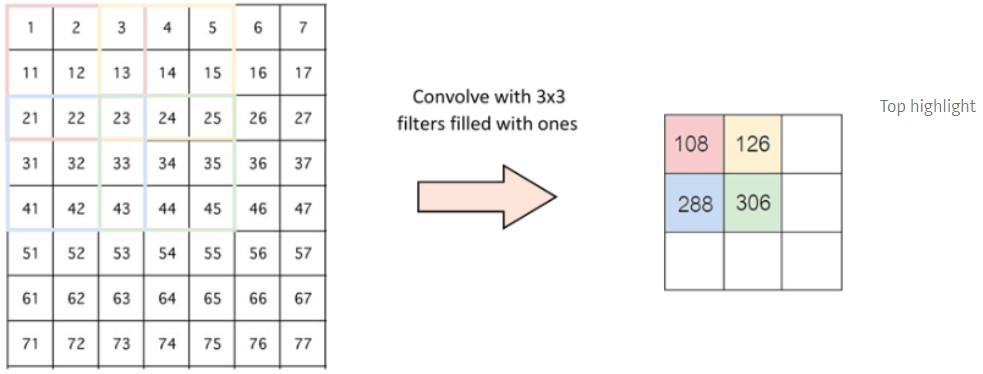
\includegraphics[width=0.63\textwidth]{2/figures/stride_cnn.jpg}
					\caption[Paso de 2 píxeles por parte de un filtro]{Paso de 2 píxeles por parte de un filtro.\\
					Fuente: \cite{tec_prabhu2018cnn}. \textit{Understanding of Convolutional Neural Network (CNN) — Deep Learning}.}
					\label{2:fig31}
				\end{center}
			\end{figure}
			
			Si, por el contrario, se desea aplicar convolución a una imagen sin afectar sus dimensiones luego de pasar por la capa de reducción, se construye bordes de ceros de n píxeles. A este tamaño de borde se le llama Relleno (\textit{pad} en inglés), por lo que el tamaño de la nueva salida se obtiene mediante la fórmula:
			
			%\begin{equcaption}[!ht]
			\begin{equation}\label{eq:outputconvwithpad}
			\phantomsection
			Salida=\frac{N-F+2*Relleno}{S}+1
			\end{equation}
			\myequations{Cálculo del tamaño de la imagen reducida con bordes rellenados con ceros}
			%\caption[Cálculo del tamaño de la imagen reducida con bordes rellenados con ceros]{Cálculo del tamaño de la imagen reducida con bordes rellenados con ceros. Fuente: \cite{tec_li2019cnn}}
			%\end{equcaption}
			
			Existen diferentes tipos de reducción \parencite{tec_prabhu2018cnn}:
			\begin{itemize}
				\item Max Pooling: Toma el elemento más grande dentro del mapa de características.
				\item Average Pooling: Toma el promedio de los elementos dentro del mapa de características.
				\item Sum Pooling: Toma la suma total de los elementos dentro del mapa de características.
			\end{itemize}
			
			\item \textbf{Capa totalmente conectada (\textit{Fully Connected Layer})}: Al final de las capas de convolución y reducción, se usan redes completamente conectadas a cada pixel considerando que cada uno como una neurona separada al igual que en una red neuronal regular \parencite{tec_lopez2016cnnTF}. En esta capa, se aplana la matriz de todas las características obtenidas anteriormente a un vector y se alinea en una capa completamente conectada a una red neuronal (Figura \ref{2:fig32}).
			\begin{figure}[h]
				\begin{center}
					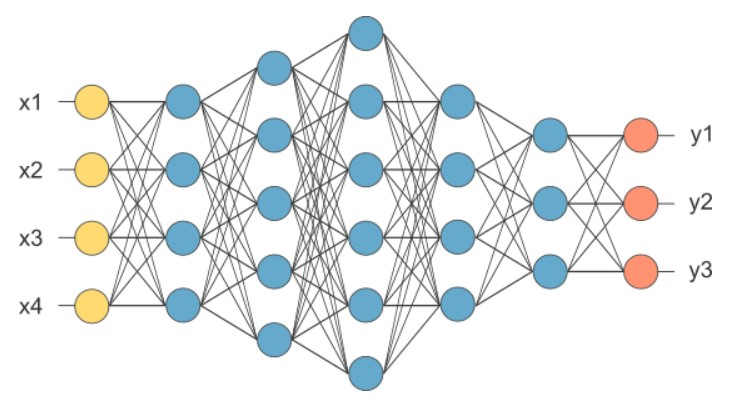
\includegraphics[width=0.65\textwidth]{2/figures/fully_conected_cnn.jpg}
					\caption[Aplanado de matrices luego de agrupar la capa]{Aplanado de matrices luego de agrupar la capa.\\
					Fuente: \cite{tec_prabhu2018cnn}. \textit{Understanding of Convolutional Neural Network (CNN) — Deep Learning}.}
					\label{2:fig32}
				\end{center}
			\end{figure}
		\end{itemize}
		Para concluir, en la Figura \ref{2:fig33} se representa la arquitectura completa de una Red Neuronal Convolucional resumiendo los conceptos anteriores.
		\begin{figure}[h]
			\begin{center}
				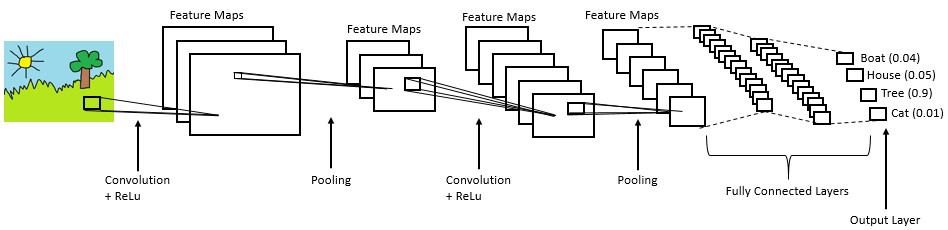
\includegraphics[width=0.95\textwidth]{2/figures/arquitectura_cnn.jpg}
				\caption[Arquitectura completa de una CNN]{Arquitectura completa de una CNN.\\
				Fuente: \cite{tec_prabhu2018cnn}. \textit{Understanding of Convolutional Neural Network (CNN) — Deep Learning}.}
				\label{2:fig33}
			\end{center}
		\end{figure}
		
		\item \textbf{Redes Neuronales Recurrentes (RNN)}: También conocidas por su nombre en inglés \textit{Recurrent Neural Networks}, se caracterizan por no tener una estructura de capas como se aprecia en la Figura \ref{2:fig34}, sino más bien por permitir conexiones entre sus neuronas de manera arbitraria para crear temporalidad y que toda la red obtenga memoria. Todo esto permite generar una red muy potente para el análisis de secuencias, entre algunos ejemplos se mencionan el análisis de textos, sonidos o video \parencite{gl_calvo2018rnn}.
		\begin{figure}[h]
			\begin{center}
				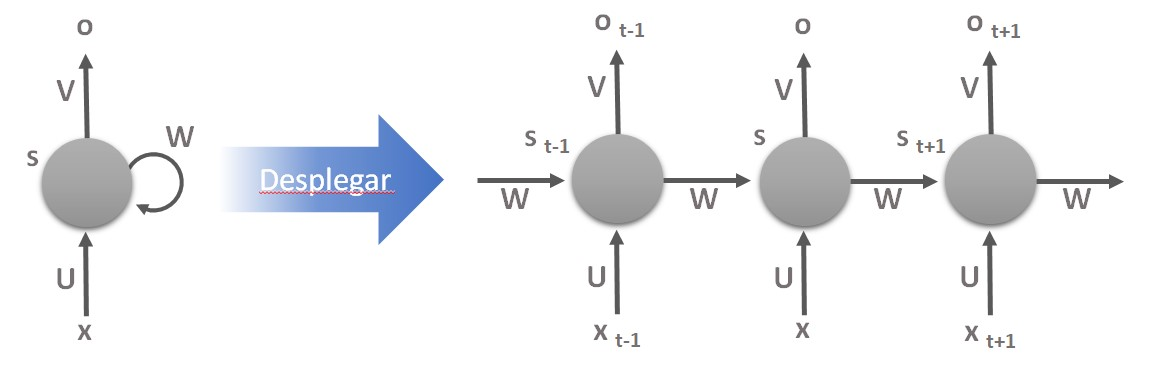
\includegraphics[width=0.85\textwidth]{2/figures/rnn_ejemplo.jpg}
				\caption[Ejemplo de red neuronal recurrente]{Ejemplo de red neuronal recurrente.\\
				Fuente: \cite{gl_calvo2018rnn}. \textit{Definición de Red Neuronal Recurrente}.}
				\label{2:fig34}
			\end{center}
		\end{figure}
	\end{itemize}
	\item \textbf{Máquina de Vectores de Soporte (SVM)}: Es un algoritmo usado para tareas de regresión y clasificación, buscando un hiperplano en un espacio N-dimensional que clasifique claramente los puntos de datos a partir de la distancia máxima entre los puntos de datos de ambas clases. Para ello, maximiza la distancia del margen proporcionando cierto refuerzo para que los puntos de datos futuros puedan clasificarse con más confianza, permitiendo distinguir 2 clases, como se muestra en la Figura \ref{2:fig35} \parencite{tec_gandhi2018svm}.
	\begin{figure}[h]
		\begin{center}
			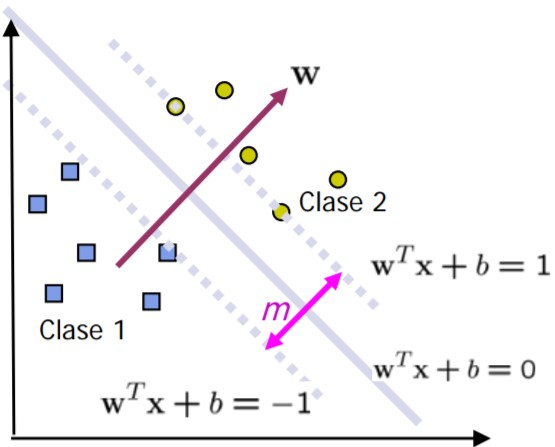
\includegraphics[width=0.45\textwidth]{2/figures/svm_hiperplano.jpg}
			\caption[Hiperplano con dos clases separadas por una distancia m]{Hiperplano con dos clases separadas por una distancia m.\\
			Fuente: \cite{tec_betancourt2005svm}. \textit{Las Máquinas de Soporte Vectorial (SVMs)}.}
			\label{2:fig35}
		\end{center}
	\end{figure}
	
	Este algoritmo tiene sus orígenes en la década de los años 60 en Rusia, desarrollados por Vapnik y Chervonenkis. Inicialmente se enfocó en el reconocimiento óptico de caracteres (OCR). Más tarde, los clasificadores de Vectores de Soporte se volvieron competitivos con los mejores sistemas disponibles en ese momento para resolver no solamente el anterior tipo de problema, sino también abarcar tareas de reconocimiento de objetos. En 1998, se publicó el primer manual de estos algoritmos por Burges. Y debido a sus grandes resultados obtenidos en la industria, actualmente se usa con frecuencia en el campo del aprendizaje automático \parencite{tec_smola2004svm}.
	
	Los vectores de soporte hacen referencia a un pequeño subconjunto de las observaciones de entrenamiento que se utilizan como soporte para la ubicación óptima de la superficie de decisión \parencite{gl_mathworks_svm}.
	
	Una Máquina de Vectores de Soporte aprende la superficie decisión de dos clases distintas de los puntos de entrada. Como un clasificador de una sola clase, la descripción dada por los datos de los vectores de soporte es capaz de formar una frontera de decisión alrededor del dominio de los datos de aprendizaje con muy poco o ningún conocimiento de los datos fuera de esta frontera. Los datos son mapeados por medio de un \textit{kernel} Gaussiano u otro tipo de \textit{kernel} a un espacio de características en un espacio dimensional más alto, donde se busca la separación máxima entre clases. Cuando es traída de regreso al espacio de entrada, la función de frontera puede separar los datos en todas las clases distintas, cada una formando un agrupamiento. Esta teoría se basa en la idea de minimización de riesgo estructural (SRM), demostrando en muchas aplicaciones tener mejor desempeño que otros algoritmos de aprendizaje tradicional como las redes neuronales para resolver problemas de clasificación \parencite{tec_betancourt2005svm}.
	
	Cabe mencionar que hay casos en que el conjunto de datos de dos clases puede ser separables no necesariamente de forma lineal. En la Figura \ref{2:fig36} se observan casos linealmente y no linealmente separables, respectivamente.
	\begin{figure}[!ht]
		\centering
		\small
		\begin{subfigure}{.5\textwidth}
			\centering
			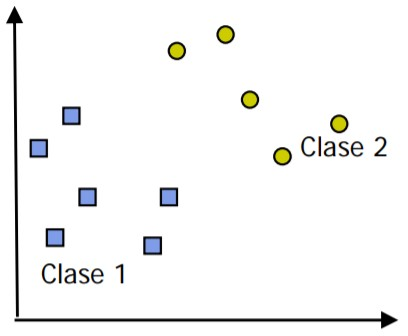
\includegraphics[width=0.6\linewidth]{2/figures/caso1_svm.jpg}
			\caption{Linealmente separable}
		\end{subfigure}%
		\begin{subfigure}{.5\textwidth}
			\centering
			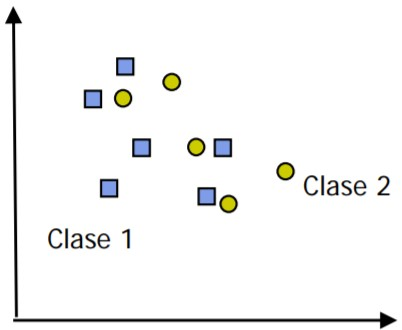
\includegraphics[width=0.6\linewidth]{2/figures/caso2_svm.jpg}
			\caption{No linealmente separable}
		\end{subfigure}
		\caption[Ejemplo de separación de 2 clases]{Ejemplo de separación de 2 clases.\\
		Fuente: \cite{tec_betancourt2005svm}. \textit{Las Máquinas de Soporte Vectorial (SVMs)}.}
		\label{2:fig36}
	\end{figure}
	
	
	Lo que se debe hacer para el primer caso es crear el hiperplano a través de una función lineal $w*z+b=0$ y, definido el par $(w,b)$, separar el punto $x_i$ según la Ecuación \ref{eq:hiperplano}:
	
	%\begin{equcaption}[!ht]
	\begin{equation}\label{eq:hiperplano}
	\phantomsection
	f(x_i) = sign(w*z+b) =
	\left\{
	\begin{aligned}
	1 \quad y_i=1\\
	-1 \quad y_i=-1
	\end{aligned}
	\right.
	\end{equation}
	\myequations{Ecuación del hiperplano para clasificar dos clases}
	%\caption[Ecuación del hiperplano para clasificar dos clases]{Ecuación del hiperplano para clasificar dos clases. Fuente: \cite{tec_betancourt2005svm}}
	%\end{equcaption}
	
	Para el segundo caso, debido a su mayor complejidad, se puede introducir algunas variables no-negativas a la función del hiperplano para hallar su valor óptimo; o también es viable utilizar una función \textit{kernel} que calcule el producto punto de los puntos de entrada en el espacio de características Z, como se aprecia en la Figura \ref{2:fig37}.
	\begin{figure}[h]
		\begin{center}
			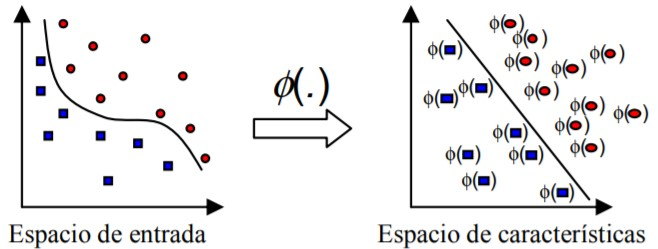
\includegraphics[width=0.75\textwidth]{2/figures/kernel_svm.jpg}
			\caption[Aplicación de un kernel para transformar el espacio de los datos]{Aplicación de un kernel para transformar el espacio de los datos.\\
			Fuente: \cite{tec_betancourt2005svm}. \textit{Las Máquinas de Soporte Vectorial (SVMs)}.}
			\label{2:fig37}
		\end{center}
	\end{figure}
	
	\item \textbf{Árboles de Decisión}: Representación visual de decisiones y toma de decisiones utilizada en la minería de datos para derivar una estrategia y alcanzar un objetivo particular. Se dibuja boca abajo con su raíz en la parte superior. Consta de nodos internos, los cuales se subdividen en ramas o bordes y su contenido, las hojas o decisiones \parencite{tec_gupta2017decisiontree}.
	
	Un árbol de decisión toma como entrada un objeto descrito a través de un conjunto de atributos y devuelve una “decisión”. Estos pueden ser discretos o continuos. La salida puede tomar cualquiera de estos dos tipos de valores; en el caso que aprenda una función tomando valores discretos se le denominará clasificación, y en el caso que la función sea continua será llamada regresión. En las clasificaciones booleanas, es decir de dos valores o binaria, clasificará como verdadero (positivo) o falso (negativo). Para alcanzar una decisión, el árbol desarrolla una serie de pruebas a través de sus nodos y las ramas que salen del nodo son etiquetadas con los valores posibles de dicha propiedad. Además, cada nodo hojas del árbol representa el valor que ha de ser devuelto si es alcanzado \parencite{bk_russell2004intart}.
	
	Por ejemplo, representando un ejemplo de este algoritmo, se ilustra en la Figura \ref{2:fig38} para decidir si se debe esperar por una mesa en un restaurante.
	\begin{figure}[h]
		\begin{center}
			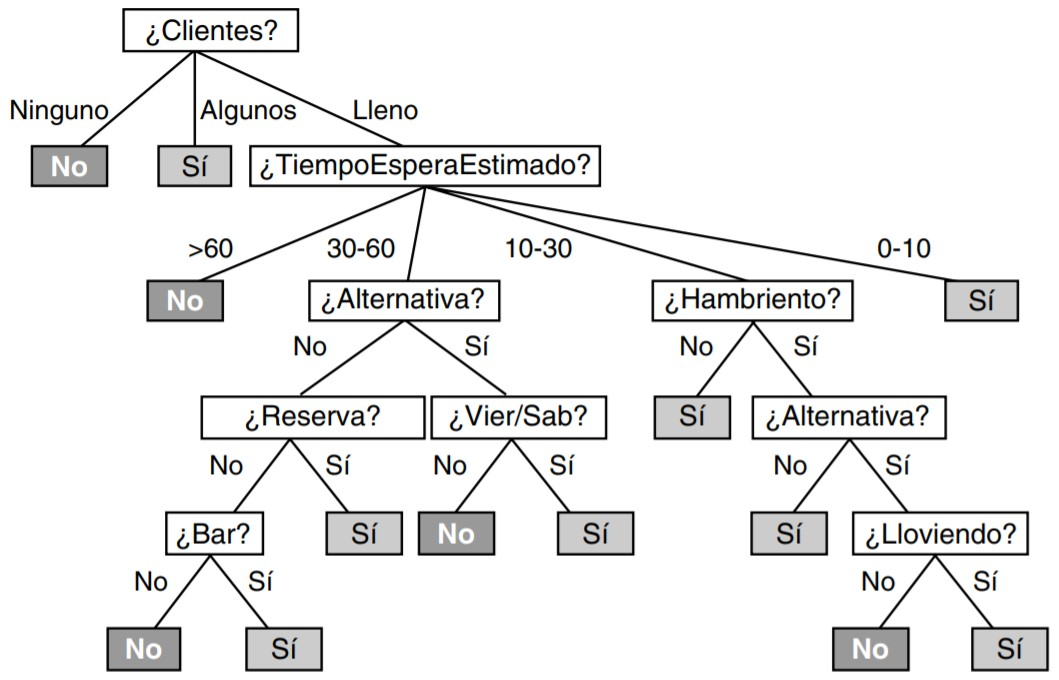
\includegraphics[width=0.85\textwidth]{2/figures/arbol_decision.jpg}
			\caption[Ejemplo del algoritmo de árbol de decisión]{Ejemplo del algoritmo de árbol de decisión.\\
			Fuente: \cite{bk_russell2004intart}. \textit{Inteligencia Artificial: Un Enfoque Moderno}. (segunda edición). (p. 745)}
			\label{2:fig38}
		\end{center}
	\end{figure}
\end{itemize}

\clearpage
\subsection{Procesamiento del Lenguaje Natural}
El Procesamiento del Lenguaje Natural (\textit{Natural Language Processing (NLP)} por su nombre en inglés) es un campo interdisciplinario que combina lingüística computacional, ciencias de la computación, ciencia cognitiva e inteligencia artifical. Investiga el uso de las computadoras para entender el lenguaje humano con el fin de realizar tareas útiles, así como lograr una interacción entre ambas partes. Algunas de estas tareas son, por ejemplo, reconocimiento de voz, comprensión del lenguaje hablado, sistemas de diálogo, análisis léxico, análisis de sentimientos, entre otros \parencite{bk_deng2018deeplearningnlp}.

Los autores \citeauthor{bk_deng2018deeplearningnlp} explican en su libro \citetitle{bk_deng2018deeplearningnlp} el desarrollo del estudio de este campo, separando desde una perspectiva histórica en 3 olas: el Racionalismo, el Empiricismo y el Aprendizaje Profundo.

El Racionalismo, nomenclatura establecida entre las décadas de los años 60s y 80s de acuerdo a los argumentos por Noam Chomsky sobre la concepción del lenguaje humano, se basa en el conocimiento de este último fijado por herencia genética y concebido desde el nacimiento. Las primeras apariciones de la aplicación de este enfoque se remontan a la década de los años 50s, donde Alan Turing, en los experimentos que se conocen como "las pruebas de Turing", intentó simular conversaciones de lenguaje natural entre un humano y un computador para generar respuestas similares a la de una persona con el fin de poder evaluar las habilidades que ellas pueden alcanzar. Durante las décadas de los 70s y 80s, los sistemas de entendimiento de lenguaje hablado y sistemas de diálogo se basaron en conjuntos de reglas, desarrollados por la ingeniería de conocimiento experto.

El Empirismo, la segunda ola, se caracterizó por la explotación del cuerpo de texto (\textit{data corpora}) y su uso con Aprendizaje Automático. Esta idea plantea que la mente humana comienza con operaciones de asociación, patrones de reconocimiento y generalización. Algunos ejemplos son el Modelo Ocultro de Markov (HMM) y los modelos de traducción de IBM.

El Aprendizaje Profundo, la tercera y última ola, se basa en el uso de estas técnicas para resolver problemas de Lenguaje Natural que el Aprendizaje Automático no puede lograr para entrenar con grandes cantidades de datos, por ejemplo. Las más comunes son las Redes Neuronales Artificiales, debido a que su configuración permite personalizar la arquitectura basada en múltiples capas e hiperparámetros para soportar el entrenamiento con volúmenes considerables. Sin embargo, pese a sus ventajas, algunas de las limitaciones que presenta son justamente este último detalle para lograr resultados estadísticos impresionantes, mucha capacidad computacional, o habilidades pobres para entender las relaciones de inter-oracional como frases o palabras progresivas dentro de una oración.

Algunas técnicas de Aprendizaje Profundo utilizados actualmente para resolver problemas de NLP comprenden modelos anteriormente mencionados como las Redes Neuronales Convolucionales (CNN) o las Redes Neuronales Recurrentes (RNN). A continuación, se detallarán algunas de las más usadas, así como las principales características y diferencias de ejemplos ya explicados bajo este contexto.

\begin{itemize}
	\item \textbf{Redes Neuronales Convolucionales} (\textit{Convolutional Neural Networks}): Entre las técnicas de minería de datos, se explicaron los conceptos y tipos de Redes Neuronales Artificiales, entre ellas, la actual mencionada. Se comentó que entre sus mayores usos se dan actualmente en el tratamiento de imágenes, problemas de clasificación a partir de estas y visión por computador. El ejemplo más popular fue ImageNet desarrollado por Yann LeCun, informático reconocido por ser el fundador de este tipo de redes, para reconocer objetos dentro de imágenes.
	
	Sin embargo, también son utilizadas para problemas de clasificación de texto. Ronan Collobert y Jason Weston fueron los pioneros de la aplicación de las CNN en tareas de procesamiento de lenguaje natural, modificando y adaptando su arquitectura y parámetros internos \parencite{bk_kamath2019deeplearning_nlp_sr}. En la Figura \ref{2:fig39} se ilustra la arquitectura de una CNN para problemas de NLP.
	\begin{figure}[!ht]
		\begin{center}
			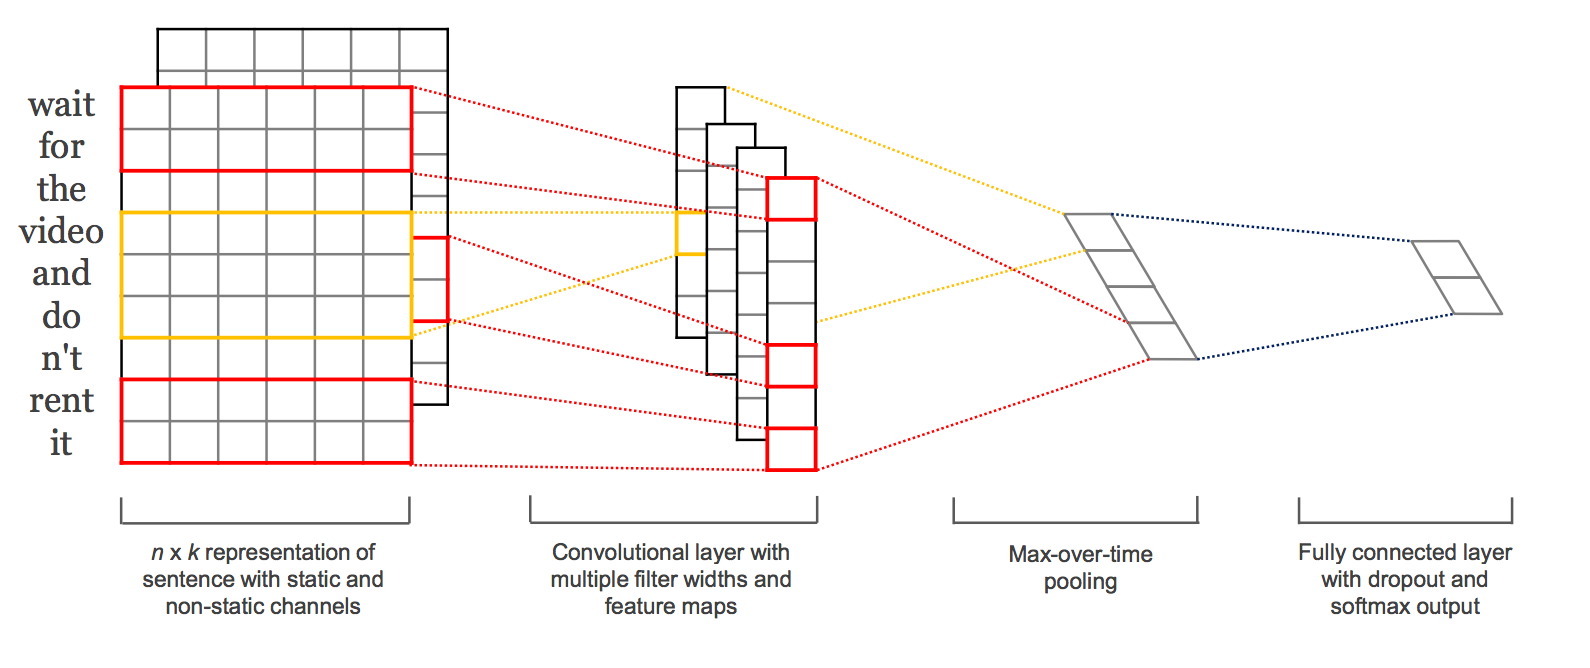
\includegraphics[width=0.95\textwidth]{2/figures/cnn_nlp.png}
			\caption[Arquitectura de modelo CNN con 2 canales para una oración de ejemplo]{Arquitectura de modelo CNN con 2 canales para una oración de ejemplo.\\
			Fuente: \cite{tec_kim2014convolutional}. \textit{Convolutional Neural Networks for Sentence Classification}. (p. 1747)}
			\label{2:fig39}
		\end{center}
	\end{figure}
	
	Una de las principales diferencias entre ambos tipos de aplicación es que las convoluciones para imágenes son bidimensionales (2d) debido a que se desplazan a través de matrices de 2 dimensiones (largo y ancho). Mientras que las convoluciones unidimensionales (1d) son muy útiles para series de tiempo y operaciones de NLP por estar conformadas por vectores, aprendiendo así patrones en la dimensión de secuencia \parencite{bk_rao2019nlp_pytorch}. En la Figura \ref{2:fig40} se observa una comparación entre ambos tipos de convolución según el tamaño de dimensión.

	\begin{figure}[!ht]
		\centering
		\small
		\begin{subfigure}{.5\textwidth}
			\centering
			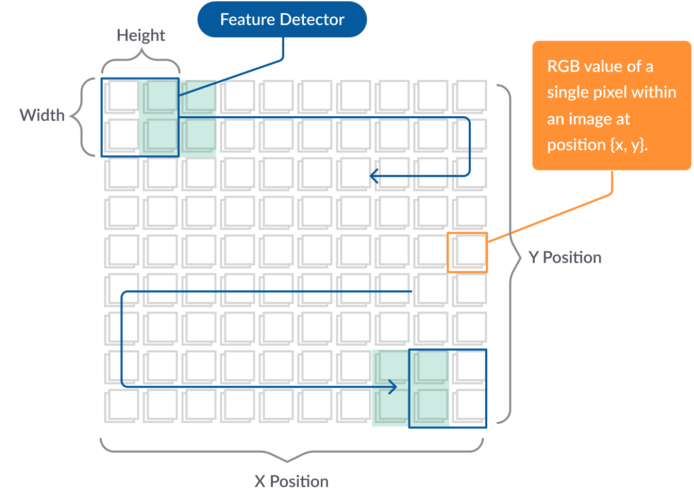
\includegraphics[width=1.00\linewidth]{2/figures/2D-convolutional-example.png}
			\caption{Convolución 2d}
		\end{subfigure}%
		\begin{subfigure}{.5\textwidth}
			\centering
			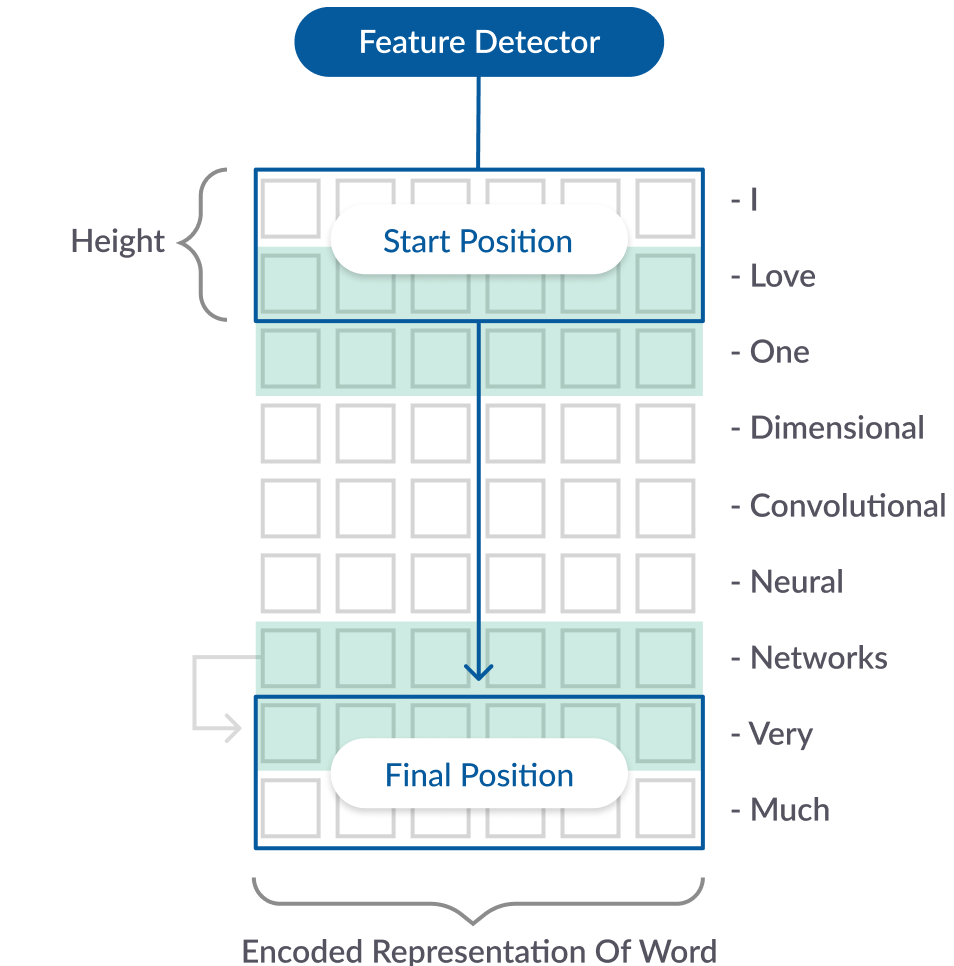
\includegraphics[width=0.85\linewidth]{2/figures/1D-convolutional-example.png}
			\caption{Convolución 1d}
		\end{subfigure}
		\caption[Diferencias entre convoluciones según su dimensión]{Diferencias entre convoluciones según su dimensión.\\
		Fuente: \cite{tec_missinglink_conv1d}. \textit{Keras Conv1D: Working with 1D Convolutional Neural Networks in Keras}.}
		\label{2:fig40}
	\end{figure}
	
	En la anterior imagen, donde cada palabra codificada se representa por un vector, un kernel de convolución de tamaño de 2 bloques (\textit{kernel\_size}) recorre toda la oración con paso (\textit{stride}) de 1 bloque.
	
	Para problemas de clasificación de texto como los que se considera en esta investigación y en algunos antecedentes con contenido textual, el proceso de la arquitectura CNN de manera general se basa en la Figura \ref{2:fig41}.
	\begin{figure}[!ht]
		\begin{center}
			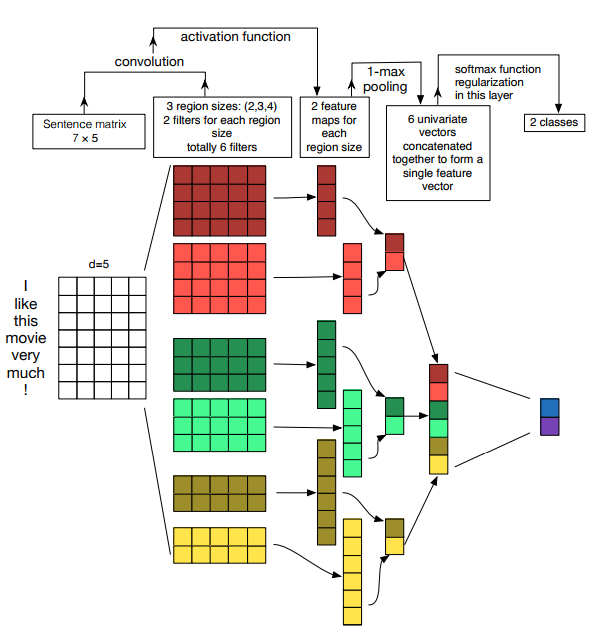
\includegraphics[width=0.60\textwidth]{2/figures/cnn_steps_for_nlp.png}
			\caption[Arquitectura de modelo CNN para clasificación de oraciones]{Arquitectura de modelo CNN para clasificación de oraciones.\\
			Fuente: \cite{tec_zhang2017cnn_sentenceclassification}. \textit{A Sensitivity Analysis of (and Practitioners’ Guide to) Convolutional Neural Networks for Sentence Classification}. (p. 256)}
			\label{2:fig41}
		\end{center}
	\end{figure}
	
	La idea general es básicamente formar vectores de palabras codificadas para generar una matriz, la cual al ser recorrida por filtros de una dimensión determinada, se obtengan mapas de características para la siguiente entrada. De cada capa resultante, se agruparán (\textit{pooling}) según el criterio del usuario (puede ser valor máximo, mínimo, promedio, etc) para generar nuevos vectores univariantes que serán concatenados y luego el valor final de predicción regularizado entre un rango dependiendo de la función de activación asignada para el problema (\textit{sigmoid} para clasificación de 2 clases o \textit{softmax} a partir de 3 clases). 
	
	\newpage
	\item \textbf{Redes Neuronales Recurrentes} (\textit{Recurrent Neural Networks}): Este tipo de redes también fue comentada brevemente en los tipos de redes neuronales más conocidas. Las RNN son muy usadas incluso también en series de tiempo, ya que los datos para estas casuísticas son secuencias, es decir, una colección ordenada de elementos. Para el caso del lenguaje humano, en donde el habla es un conjunto de secuencia de palabras llamadas fonemas, se busca predecir la siguiente palabra en una oración dada a partir de un elemento dependiente, en este caso, las palabras previas \parencite{bk_rao2019nlp_pytorch}. Como ejemplos de estos casos de uso más comunes se mencionan a los motores de búsqueda en navegadores o sitios web, traductores, entre otros.
	
	Según \cite{bk_brownlee2017deeplearning_nlp}, las RNN generalmente más usadas son los siguientes 3 tipos:
	\begin{itemize}
		\item \textbf{RNN Simple} (\textit{Elman Network} o S-RNN): Son el tipo de redes neuronales recurrentes más básicas, propuesto por Jeffrey L. Elman en 1990, cuya arquitectura se caracteriza por la secuencia de elementos, como en la Figura \ref{2:fig34}.
		Las S-RNN proporcionan resultados sólidos para el etiquetado de secuencias, así como para el modelado del lenguaje.
		
		La ecuación para representar un estado determinado en una RNN toma la siguiente forma:
		
		%\begin{equcaption}[!ht]
		\begin{equation}\label{eq:srnn}
		\phantomsection
		s_i = R_{SRNN}(x_i, s_{i-1}) = g([s_{i-1};x_i]W+b)
		\end{equation}
		\myequations{Fórmula para determinar un estado en una S-RNN}
		%\caption[Fórmula para determinar un estado en una S-RNN]{Fórmula para determinar un estado en una S-RNN. Fuente: \cite{bk_brownlee2017deeplearning_nlp}}
		%\end{equcaption}
		
		Donde se observa que un estado depende de la información del estado previo.
		
		\item \textbf{Memoria Larga a Corto Plazo} (\textit{Long-Short Term Memory} o LSTM): Este modelo fue desarrollado para encargarse del problema de los gradientes que desaparecen de la RNN Simple, que limitaba más adelante el entrenamiento de las RNN profundas.
		
		Según el mismo autor, este problema surge debido a que los gradientes incluyen la multiplicación repetida de la matriz W (de la Ecuación \ref{eq:srnn}), haciendo que los valores desaparezcan.
		
		Esta arquitectura divide el vector de un estado observado $s_i$ en dos mitades, donde una es tratada como “celdas de memoria” y la otra es la memoria de trabajo. Las del primer grupo tienen como función preservar la memoria, así como también los gradientes de error, a lo largo del tiempo. Son controladas mediante componentes de puerta diferenciables, que son funciones matemáticas suaves simuladoras puertas lógicas. En cada estado de entrada, se utiliza una puerta para decidir qué cantidad de la nueva entrada se debe escribir en la memoria.
		
		La arquitectura LSTM es actualmente la más exitosa dentro de las RNN. Un ejemplo de su representación puede ilustrarse en la Figura \ref{2:fig42}.
		
		\begin{figure}[!ht]
			\begin{center}
				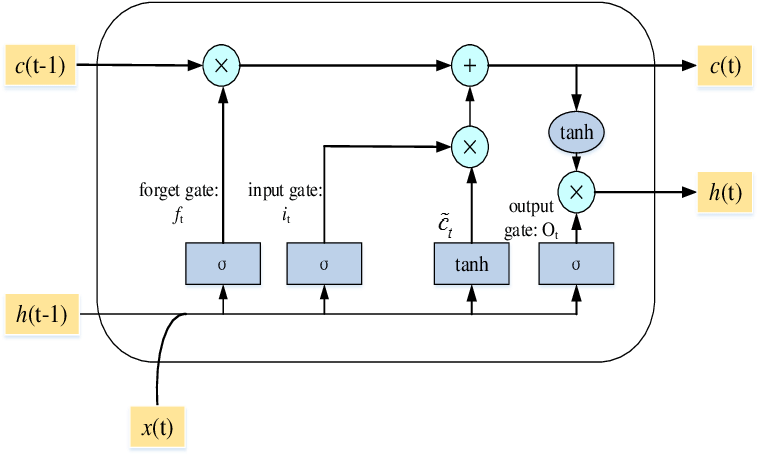
\includegraphics[width=0.65\textwidth]{2/figures/lstm.png}
				\caption[Arquitectura de una LSTM]{Arquitectura de una LSTM.\\
				Fuente: \cite{tec_yuan2019lstm}. \textit{Nonlinear Dynamic Soft Sensor ModelingWith Supervised	Long Short-Term Memory Network}. (p. 2)}
				\label{2:fig42}
			\end{center}
		\end{figure}
	
		En donde $x$ son las entradas, $c_{t-1}$ y $c_{t}$ los estados de la celda, y $h_{t-1}$ y $h_{t}$  las salidas.
		
		Una variante muy útil de las RNN son las RNN Bidireccionales (\textit{Bidirectional RNN} o \textit{BiRNN}). Mientras una red neuronal recurrente toma una palabra del pasado para predecir el siguiente, las bidireccionales permiten mirar arbitrariamente lejos tanto al pasado como al futuro dentro de una secuencia \parencite{bk_goldberg2017nn_nlp}.
		La ventaja que se logra a partir de estas características es que, por ejemplo, el modelo puede identificar y discernir mejor en la predicción de la siguiente palabra en el caso de existir 2 o más secuencias idénticas (problema de reconocimiento de entidades nombradas) al lograr conocer más información.
		
		\cite{tec_ng2018bidirectionalRNN}, fundador de Coursera, DeepLearning.AI, Landing AI y Google Brain, explica lo anterior con el siguiente ejemplo como parte del curso Redes Neuronales Recurrentes:
		
		Sean las oraciones \textit{He said, “Teddy bears are on sale!”} y \textit{He said, “Teddy Roosevel was a great President!”}, se desea saber si \textit{Teddy} es parte del nombre de una persona. El problema es que se cuenta con 2 oraciones cuya secuencia inicial de 3 palabras resultan ser las mismas, pero con distinto panorama posterior a estas. Por ello, la red es duplicada pero con orden de secuencia invertida y colocada en paralelo con la original para que cada una de las nuevas capas conecten sus salidas con las pre-existentes y originen una nueva predicción que toma información previa y posterior.
		
		Bajo la misma premisa, pero con la oración de ejemplo \textit{The brown fox jumped over the dog}, se representa la arquitectura de una BiRNN en la Figura \ref{2:fig43}.
		
		\begin{figure}[!ht]
			\begin{center}
				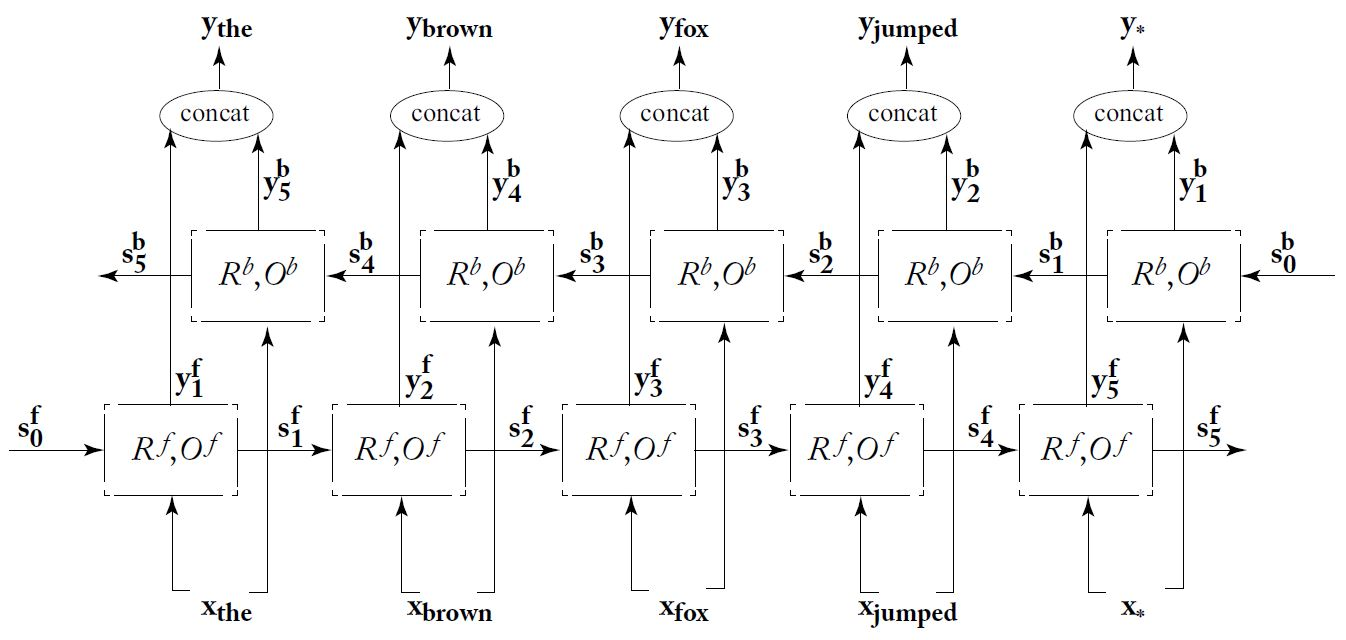
\includegraphics[width=0.90\textwidth]{2/figures/birnn_architecture.jpg}
				\caption[Representación de arquitectura BiRNN de la palabra \textit{jumped} en la oración]{Representación de arquitectura BiRNN de la palabra \textit{jumped} en la oración.\\
				Fuente: \cite{bk_goldberg2017nn_nlp}. \textit{Neural Network Methods for Natural Language Processing}. (p. 171)}
				\label{2:fig43}
			\end{center}
		\end{figure}
		
		Como parte de las BiRNN, se encuentra la LSTM Bidireccional (\textit{Bidirectional LSTM} o \textit{BiLSTM}), mejora de la LSTM, que sobresale particularmente en la representación de palabras en la secuencia junto con sus contextos, capturando la palabra y las incontables posibilidades existentes a su alrededor \parencite{bk_deng2018deeplearningnlp}.
		
		\item \textbf{Unidad Recurrente Cerrada} (\textit{Gated Recurrent Unit} o GRU): Este modelo se desarrolló con la intención de simplificar la LSTM debido a su complejidad. Al igual que esta, consiste en un mecanismo de puertas pero en menor cantidad y sin un componente de memoria separada (ver Figura \ref{2:fig44}). La red GRU muestra ser efectiva en modelamiento de lenguaje y máquina traductora \parencite{bk_goldberg2017nn_nlp}.
		
		\begin{figure}[!ht]
			\begin{center}
				\includegraphics[width=0.95\textwidth]{2/figures/lstm_vs_gru.png}
				\caption[Comparación entre arquitecturas LSTM y GRU]{Comparación entre arquitecturas LSTM y GRU.\\
				Fuente: \cite{tec_phi2018gru}. \textit{Illustrated Guide to LSTM’s and GRU’s: A step by step explanation}.}
				\label{2:fig44}
			\end{center}
		\end{figure}
		
		Sin embargo, al compararse los resultados entre estos 3 tipos de modelos, por lo general el mejor desempeño tiene la LSTM \parencite{bk_brownlee2017deeplearning_nlp}.
	\end{itemize}
	
	\item \textbf{Modelo Secuencia a Secuencia} (\textit{Sequence-to-Sequence Model} o \textit{Seq2seq Model}): También conocida como \textit{Encoder-Decoder} (Codificador-Decodificador por su traducción al español), es un tipo de generador de lenguaje natural (\textit{Natural Language Generation} o NLG) usado comúnmente para traducción (por ejemplo, Google Traductor). Se basa en 2 capas LSTM, en donde la primera es usada para codificar la oración de entrada en un “vector de pensamiento”, y la otra para decodificar en una respuesta (ver Figura \ref{2:fig45}) \parencite{bk_deng2018deeplearningnlp}.
	
	\begin{figure}[!ht]
		\begin{center}
			\includegraphics[width=0.67\textwidth]{2/figures/encoder-decoder.jpeg}
			\caption[Arquitectura de un modelo Seq2seq]{Arquitectura de un modelo Seq2seq.\\
			Fuente: \cite{tec_kostadinov2019seq2seq}. \textit{Understanding Encoder-Decoder Sequence to Sequence Model}.}
			\label{2:fig45}
		\end{center}
	\end{figure}	
\end{itemize}

\newpage
El contenido textual que se usa en los modelos anteriores debe ser pre-procesada previamente. El texto en sí no puede ser incluido tal cual en los modelos de Aprendizaje Automático o Aprendizaje Profundo sin antes ser limpiado \parencite{bk_brownlee2017deeplearning_nlp}. Python ofrece una librería para trabajar y modelar texto llamada Natural Language Toolkit o NLTK. Algunas de las funciones disponibles se encuentran separación de texto en oraciones, separación en palabras o tokenización, eliminación de signos de puntuación, eliminación de palabras de parada (\textit{stop words}), reducción de palabras hacia su forma raíz (\textit{stemming}), retorno de palabras hacia su base o forma diccionario (\textit{lemmatization}).

Suprimir contenido como signos de puntuación, caracteres especiales, palabras de parada, enlaces web, entre otros, ayuda a reducir la cantidad de vectores innecesarios para las representaciones de palabras que se utilizan en la fase de entrenamiento. Para ello, la secuencia de entrada debe dividirse en \textit{tokens}, que pueden ser una palabra, oración, párrafo.

NLTK ofrece más de una alternativa para la tokenización, como por ejemplo, \textit{WhitespaceTokenizer} (elimina espacios en blanco para separar palabras y signos de puntuación en una oración, estos últimos no son independientes), \textit{TreebankWordTokenizer} (separa palabras y signos de puntuación en una oración de manera independiente) y \textit{WordPunctTokenizer} (funciona igual que TreebankWordTokenizer pero no distingue contracciones en idiomas como el inglés). La elección de alguna de estas depende del objetivo que busque el usuario. Asimismo, la reducción de palabras hacia su raíz (llamada \textit{stem}) permite suprimir los prefijos o sufijos agregados a una palabra. Sin embargo, presenta problemas en formas irregulares, generando “No palabras”. El retorno de palabras hacia su forma base (llamada \textit{lemma}), por su lado, convertir palabras conjugadas en distintas variantes de tiempo. Aún así, no todas las formas pueden ser reducidas. La finalidad de estos 2 últimos es reducir una palabra a su forma más primitiva (expresiones regulares) para generar un diccionario homogéneo \parencite{tec_zimovnov2018text_preprocessing}.

Luego de la limpieza de texto, el nuevo conjunto de datos debe representarse como vectores. Dentro de las modalidades más usadas para representación de palabras se encuentran:
\begin{itemize}
	\item \textbf{Incrustación de palabra} (\textit{Word Embedding}): Es una representación aprendida para texto en donde las palabras con el mismo significado tienen una similar representación. La principal ventaja que presenta es la baja dimensionalidad de vectores a nivel computacional, ya que una palabra individual se representa como vectores de valor real en un espacio vectorial predefinido, a diferencia de otros métodos de muy alta dimensionalidad como la codificación en caliente (\textit{one hot encoding}) o la bolsa de palabras (\textit{bag-of-words}), en donde distintas palabras presentan diferentes representaciones \parencite{bk_brownlee2017deeplearning_nlp}.
	
	Algunos de los algoritmos destacados de este grupo son:
	\begin{itemize}
		\item \textbf{Capa de incrustación} (\textit{Embedding Layer}): Consiste en una incrustación de palabras que aprende con un modelo de red neuronal. En esta capa, se especifica el tamaño del espacio vectorial (dimensiones), donde los vectores inicializan con pequeños valores aleatorios. La capa se utiliza en el extremo frontal de la red, es decir, luego de la capa de entrada, y es ajustada de forma supervisada mediante el algoritmo de propagación hacia atrás. Puede recibir palabras codificadas, en donde cada una se representa por un código, o codificación en caliente, la cual presenta mayor dimensión. Si se utiliza un Perceptrón Multicapa (MLP), los vectores de palabras son concatenados antes de entrar al modelo. En el caso se use una RNN, cada palabra será tomada como una entrada en una secuencia \parencite{bk_brownlee2017deeplearning_nlp}. Como se observa en la Figura \ref{2:fig46}, la capa de incrustación toma como entrada a la matriz de incrustación y la transforma en un vector tridimensional de \textit{n} registros.
		
		\begin{figure}[!ht]
			\begin{center}
				\includegraphics[width=0.67\textwidth]{2/figures/embedding_layer.jpg}
				\caption[Ejemplo de funcionamiento de una capa de incrustación]{Ejemplo de funcionamiento de una capa de incrustación.\\
				Fuente: \cite{tec_chengwei2018embedding}. \textit{Simple Stock Sentiment Analysis with news data in Keras}.}
				\label{2:fig46}
			\end{center}
		\end{figure}
		
		\item \textbf{Palabra a vector} (\textit{Word2Vec}): Se trata de un método estadístico, desarrollado en el 2013 por Tomas Mikolov, cuya finalidad es de aprender eficientemente una incrustación de palabras independientes de un corpus de texto, incluso si este y sus dimensiones son más grandes. En este trabajo se involucró el análisis de los vectores aprendidos y la exploración de la matemática vectorial para representar palabras. Para entender estos conceptos, se ilustra bajo el ejemplo de la analogía “\textit{Rey es a Reina como hombre es a mujer}”, en donde se evidencia la relación sintáctica y semántica capturada por su proximidad vectorial \parencite{bk_brownlee2017deeplearning_nlp}. La Figura \ref{2:fig47} grafica las palabras relacionadas en un espacio vectorial gracias al algoritmo.
		
		\begin{figure}[!ht]
			\begin{center}
				\includegraphics[width=0.95\textwidth]{2/figures/word2vec.png}
				\caption[Incrustaciones de palabras por Word2Vec]{Incrustaciones de palabras por Word2Vec.\\
				Fuente: \cite{tec_bujokas2020word2vec}. \textit{Creating Word Embeddings: Coding the Word2Vec Algorithm in Python	using Deep Learning}.}
				\label{2:fig47}
			\end{center}
		\end{figure}
		
		\item \textbf{Vectores globales para representación de palabra} (\textit{GloVe}): Es un algoritmo de aprendizaje no supervisado para obtener representaciones vectoriales de palabras. Es una extensión del método Word2Vec, desarrollado en 2014 por Jeffrey Pennington como proyecto de código abierto en la Universidad Stanford. Las representaciones de palabras del modelo de espacio vectorial clásico se desarrollaron utilizando técnicas de factorización matricial como el Análisis semántico latente (LSA), con el cual combina sus características de aprendizaje adoptadas de Word2Vec, logrando un modelo de aprendizaje con mejor performance para incrustación de palabras \parencite{gl_pennington2014glove}. GloVe dispone en su web distintos vectores de palabras pre-entrenados, entre ellas, un vocabulario de más de 400 mil palabras, hasta 4 opciones de matrices con distintas dimensiones, y 6 billones de tokens extraídos de Wikipedia (2014) y Gigaword (5ta edición) de la Universidad de Pensilvania, así como datas públicas extraídas de mayor tamaño. La Figura \ref{2:fig48} ilustra ejemplos de palabras  relacionadas en un espacio vectorial gracias al algoritmo. La relación semántica (palabras clasificadas en un mismo grupo) entre ellas se aprecia por la cercanía en su el eje Y. Mientras que aquellos señalados con líneas horizontales en su eje X se encuentran asociadas por analogías, como por ejemplo, género, geolocalización, compañía, grados del adjetivo, entre otros.
		
		\begin{figure}[!ht]
			\centering
			\small
			\begin{subfigure}{.55\textwidth}
				\centering
				\includegraphics[width=0.85\linewidth]{2/figures/glove_man-woman.jpg}
				\caption{hombre - mujer}
			\end{subfigure}%
			\begin{subfigure}{.55\textwidth}
				\centering
				\includegraphics[width=0.85\linewidth]{2/figures/glove_company-ceo.jpg}
				\caption{compañía - CEO}
			\end{subfigure}
			\begin{subfigure}{.55\textwidth}
				\centering
				\includegraphics[width=0.85\linewidth]{2/figures/glove_comparative-superlative.jpg}
				\caption{comparativo - superlativo}
			\end{subfigure}%
			\begin{subfigure}{.55\textwidth}
				\centering
				\includegraphics[width=0.85\linewidth]{2/figures/glove_city-zipcode.jpg}
				\caption{ciudad - código postal}
			\end{subfigure}
			\caption[Incrustaciones de palabras por GloVe]{Incrustaciones de palabras por GloVe.\\
			Fuente: \cite{tec_pennington2014glove}. \textit{GloVe: Global Vectors for Word Representation}.}
			\label{2:fig48}
		\end{figure}
		
	\end{itemize}

	\item \textbf{Bolsa de palabras} (\textit{Bag-of-Words} o \textit{BoW}): Consiste en una forma de extraer características de textos implicando un vocabulario de palabras conocidas y una métrica de presencia de éstas. Se le denomina Bolsa de palabras ya que no considera el orden o la estructura de las palabras dentro del documento, sólo se enfoca en conocer su presencia. El algoritmo relaciona la similitud entre documentos si tienen contenido similar \parencite{bk_brownlee2017deeplearning_nlp}. Por ejemplo, en la Figura \ref{2:fig49} el algoritmo cuantifica la frecuencia cada palabra individual dentro de un documento sin importar su orden. De esta manera, los relaciona a partir de su recurrencia en todos ellos.
	
	\begin{figure}[!ht]
		\begin{center}
			\includegraphics[width=0.90\textwidth]{2/figures/bow_example.png}
			\caption[Ejemplo de funcionamiento de bolsa de palabras]{Ejemplo de funcionamiento de bolsa de palabras.\\
			Fuente: \cite{tec_zhou2019bow}. \textit{A Simple Explanation of the Bag-of-Words Model}.}
			\label{2:fig49}
		\end{center}
	\end{figure}
	
	\item \textbf{Frecuencia del término - Frecuencia inversa del documento} (\textit{TF-IDF}): Es un algoritmo que también contabiliza palabras pero que resaltan aquellas más significativas para calcular sus pesos correspondientes. Se compone por la frecuencia que una palabra aparece en un documento, y la frecuencia inversa del documento, el cual reduce la escala de palabras que aparecen mucho en los documentos \parencite{bk_brownlee2017deeplearning_nlp}.
	
	\begin{figure}[!ht]
		\begin{center}
			\includegraphics[width=1.00\textwidth]{2/figures/tfidf_example.png}
			\caption[Ejemplo de funcionamiento de TF-IDF]{Ejemplo de funcionamiento de TF-IDF.\\
				Fuente: \cite{tec_brinton2020ngrams}. \textit{Python for Data Science: n-grams and basic natural language processing}.}
			\label{2:fig50}
		\end{center}
	\end{figure}
	
	Su peso se calcula bajo la siguiente fórmula:	
	%\begin{equcaption}[!ht]
	\begin{equation}\label{eq:tfidf}
	\phantomsection
	TF-IDF_{(n,d)}=TF_{(n,d)}*IDF_{(n)}
	\end{equation}
	\myequations{Fórmula de TF-IDF}
	%\caption[Fórmula de TF-IDF]{Fórmula de TF-IDF. Fuente: \cite{tec_hamdaoui2019tfidf}}
	%\end{equcaption}
	Donde:
	\begin{conditions}
		TF_{(n,d)}	&	número de veces que el término \textit{t} aparece en un documento \textit{d} \\
		IDF_{(n)}	&	$\log{\frac{1+n}{1+df_{(d,n)}}+1}$	\\
		n			&	número de documentos	\\
		df_{(d,n)}	&	frecuencia de documentos \textit{d} que contienen el término \textit{t}
	\end{conditions}
	
\end{itemize}

\section{Marco Conceptual}
\subsection{Crowdfunding}
El financiamiento colectivo o crowdfunding es un sistema que, utilizando internet como base de operaciones, busca generar una respuesta económica activa en el usuario \parencite{cr_lopezgolan2017crowdfunding}.

Combinando ideas de microfinanzas y crowdsourcing, el crowdfunding es la práctica de financiar una empresa o un proyecto al recaudar muchas pequeñas cantidades de dinero de un gran número de personas. Este mecanismo de financiamiento ha sido recibido por los recaudadores de fondos, el público en general y los formuladores de políticas. La industria de crowdfunding ha crecido rápidamente en los últimos años, así como el crecimiento exponencial del número de plataformas de crowdfunding, el número de proyectos expuestos allí y el número de capital total recaudado en esos sitios web \parencite{cr_xuefeng2018chcrowdplatf}.

La cantidad de grupos de crowdfunding varía según distintos autores. Según \citeauthor{cr_hollas2013crwd}, se clasifican en 4 modelos: basado en donaciones, recompensas, capital y deuda. \citeauthor{cr_colgren2014risecrwd} reafirma lo anterior con la variante de crédito en vez de capital y por su lado, \citeauthor{cr_collins2014crwd}, préstamo por deuda. Mientras que \citeauthor{cr_lee2018fintech} solo consideran principalmente al crowdfunding basado en recompensas, donaciones y capital. El crowdfunding basado en capital social se encuentra actualmente limitado en los Estados Unidos debido a que la Regulación D de la Ley de Valores de 1933 prohíbe la participación de muchos potenciales inversionistas y los obliga a tener un ingreso anual mayor a \$ 200,000 o más de \$ 1 millón en patrimonio neto \parencite{cr_lichtig2015crowdfunding}.

El modelo basado en donaciones se refiere a la recaudación de fondos a través de la Web 2.0, en el cual los patrocinadores no esperan recompensas materiales a cambio sino más bien una recompensa social. Por el contrario, el modelo basado en recompensas ofrece compensación tanto material como inmaterial y representa hoy en día el modelo de crowdfunding más frecuente. Los financiadores, por un lado, pueden verse beneficiados de la venta anticipada, recibiendo el proyecto o producto financiado antes de su publicación o entrada al mercado al mejor precio. Los proyectos que pertenecen a esta categoría a menudo son organizaciones sin fines de lucro \parencite{cr_kraus2016crowdfunding_strategies}.

Además de los tipos mencionados en el párrafo anterior, \citeauthor{cr_collins2014crwd} también afirma que el crowdfunding se puede dividir en 2 tipos de modelo de negocio \parencite{cr_lee2019crwdfactors}:
\begin{itemize}
	\item El \textbf{modelo “Todo o Nada”} (\textit{All-Or-Nothing} (AON) en inglés), el cual un proyecto logra ser financiado si es que alcanza o sobrepasa la meta durante el periodo de campaña. A partir de esto, el creador tiene como principal objetivo motivar a los patrocinadores. En caso de no lograrse el cometido, los montos aportados al proyecto serán devueltos, significando un riesgo menor para ellos. Esto, asimismo, permite evaluar a los dueños las variables de la campaña para apostar por un algún cambio o decisión que le permita encaminar al éxito del financiamiento. Hasta febrero del 2019, el ratio promedio de proyectos financiados exitosamente en Kickstarter (considerando todas las categorías de la plataforma) fue de 37\%. Sin embargo, aunque parezca un indicador con baja performance, según la misma compañía, el 82\% de los proyectos que alcanzan el 20\% de su meta son financiados exitosamente. 
	\item El \textbf{modelo “Mantener todo”} (\textit{Keep-In-All} (KIA) en inglés), muy similar al anterior, con la única diferencia que el creador del proyecto mantiene todo el dinero financiado después de acabar el plazo de días sin importar si alcanza o no la meta establecida. En contraste con el modelo AON, este presenta un ratio menor de éxito. Asimismo, la plataforma de crowdfunding de este tipo de modelo más popular es Indiegogo, que viene funcionando desde el 2008.
\end{itemize}

Algunos factores clave, relacionados a la eficiencia del proceso y la retención de clientes durante la campaña, que afectan a un crowdfunding exitoso son \parencite{cr_lee2019crwdfactors}:
\begin{itemize}
	\item Seleccionar una plataforma correcta. Esta normalmente depende de los objetivos reales que busca el creador del proyecto durante la campaña. En el anterior punto se mencionaron las dos principales dirigidas a un tipo de modelo de negocio en particular cada una.
	\item Crear un proyecto atractivo. Las personas normalmente se motivan a contribuir económicamente por algún proyecto que sea de su interés. Para ello, deben ser fáciles de entender en general.
	\item Ofrecer diferentes opciones de recompensa. Estas pueden ir más allá de lo económico. Influirá mucho el nivel de creatividad que tenga el creador para llamar la atención del público.
	\item Promocionar un video. Además del contenido que pueda tener un proyecto, ayuda mucho el apoyo de material audiovisual que complemente o explique brevemente la descripción de este. Brinda una mejor impresión y además, para las generaciones más jóvenes, es más útil que leer un enunciado extenso.
\end{itemize}

\subsection{Kickstarter}
Kickstarter, desde su inicio en 2009, es una plataforma de financiamiento de proyectos creativos de todo tipo, los cuales incluyen películas, juegos, música, arte, diseño y tecnología. Actualmente, se han registrado más de 162 mil proyectos realizados, 16 millones de contribuyentes y 4,3 miles de millones de dólares fondeados \parencite{cr_kickstarter_about}. La plataforma utiliza un modelo de financiamiento llamado “Todo o Nada” (AON), el cual consiste en que, si un proyecto no alcanza su meta de financiamiento en un determinado plazo de tiempo, no se realiza ninguna transacción de fondos, como se explicó en el anterior punto \parencite{cr_kickstarter_founding}. Si bien los patrocinadores apoyan estos proyectos por motivos personales y distintos para hacerlos realidad, ellos no obtienen la propiedad o los ingresos de los proyectos que financian, sino que los creadores conservan la totalidad de su trabajo \parencite{cr_kickstarter_press}.

\begin{figure}[!ht]
	\begin{center}
		\includegraphics[width=0.70\textwidth]{2/figures/kickstarter_project.jpg}
		\caption[Ejemplo de proyecto vigente en Kickstarter]{Ejemplo de proyecto vigente en Kickstarter.\\
			Fuente: \cite{cr_perry2012kickstarterproject}. \textit{The New Project Page}.}
		\label{2:fig52}
	\end{center}
\end{figure}

\subsection{Proyecto}
Un proyecto es un esfuerzo temporal que se lleva a cabo para crear un producto, servicio o resultado único. La naturaleza temporal de los proyectos indica un principio y un final definidos, y que el propósito se alcanza cuando se logran los objetivos del proyecto o cuando este es terminado por no cumplir sus objetivos, o cuando ya no existe la necesidad inicial que dio origen al mismo \parencite{bk_pmi2017pmbokguide}.

A partir de este concepto enunciado por el PMI, se entiende que un proyecto parte de una idea que un individuo o conjunto de individuos tienen en mente para convertirla en realidad con el fin de responder a una necesidad.

En Kickstarter, los proyectos que pueden ser financiados deben pertenecer a las siguientes categorías: Arte, Cómics, Artesanías, Baile, Diseño, Moda, Cine y vídeo, Comida, Juegos, Periodismo, Música, Fotografía, Publicaciones, Tecnología, y Teatro. Cualquier tipo de persona puede contribuir al mismo desde ser patrocinadores hasta formar parte de las principales referencias \parencite{cr_kickstarter_learn}.

Dentro de las normas internas de la plataforma para la creación de proyectos se especifica que cada proyecto debe resultar ser totalmente nuevo, original e innovador que pueda ser compartido con el público, así como haber sido presentados de forma honesta y clara. En adición a esto, también se menciona que las recaudaciones que se darán no podrán ser otorgadas a obras benéficas sino cumplir con el objetivo de llevar a cabo el proyecto planteado, al igual que está prohibido asimismo del ofrecimiento de incentivos financieros como resultado \parencite{cr_kickstarter_rules}.


\subsection{Campaña}
Una campaña puede abarcar diversos términos si es que se busca su concepto en fuentes confiables como la Real Academia Española debido al alcance y empleabilidad del mismo. El significado más próximo que la RAE enuncia sobre campaña es la de un “conjunto de actos o esfuerzos de índole diversa que se aplican a conseguir un fin determinado” \parencite{gl_rae}. Para el actual contexto, el término se refiere específicamente a la campaña publicitaria, la cual se define como una estrategia diseñada y ejecutada en diferentes medios para obtener objetivos de notoriedad, ventas y comunicación de una determinada marca o producto a través del uso de la publicidad \parencite{tec_cyberclic_campaign}.

En la plataforma de Kickstarter, existen personas que tienen ideas y proyectos en mente, buscando financiarlos en el sitio web. Para lograr su objetivo y siguiendo la regla del “todo o nada”, estos individuos realizan eventos de promoción para atraer entre personas conocidas suyas y cibernautas en general. A esta serie de eventos de promoción se le conoce como campañas. Las campañas exitosas se basan en que un determinado proyecto alcanza a ser financiado en el tiempo estimado gracias a algunas de las siguientes características \parencite{cr_kickstarter_intro}:

\begin{itemize}
	\item Logran ser claros y concisos sobre lo que su proyecto busca alcanzar al ser financiado. Se definen bien las características del proyecto mediante detalles en la descripción, videos e imágenes precisas.
	\item Indican los beneficios y recompensas que los patrocinadores obtendrán si es que la campaña es exitosa y el proyecto se financia.
	\item Atrae e interactúa con una gran cantidad de público, manteniendo constante comunicación acerca de actualizaciones y novedades de la campaña y resolviendo dudas que puedan darse.
	\item Se estiman costos de manera eficiente que pueden ser solventados para cubrir más allá del proyecto una vez financiado, incluido los que se originan para la entrega del producto a los patrocinadores. Se logra convencerlos.
\end{itemize}

El autor \cite{cr_yu2017kickstarter_course} también complementa lo anterior con las siguientes estrategias para empezar a realizar la campaña:

\begin{itemize}
	\item Además de estimar los costos, se debe contar con un buffer en caso ocurra un imprevisto. Se puede determinar la meta a través de la fórmula (Gastos + Buffer) x Alcance.
	\item Un proyecto con video tiene 50\% de chance de tener éxito. El promedio de su duración debería ser de 3.38 minutos, aunque el público presta más atención hacia aquellos que duran poco. El vídeo debe contener y responder las siguientes preguntas:
	\begin{itemize}
		\item ¿Qué hace memorable al proyecto?
		\item ¿Cómo se verá el proyecto?
		\item ¿Por qué se está creando el producto?
		\item ¿Por qué se necesita?
		\item ¿Por qué es importante que el proyecto exista?
		\item ¿Por qué se debe ser creador?
		\item ¿Por qué deben escoger la compañía?
		\item ¿Cómo se proveerá una solución?
		\item ¿Cómo funciona la solución?
	\end{itemize}
	Es importante destacar las estadísticas del problema que se piensa resolver al inicio del video ya que el primer minuto resulta ser el lapso de tiempo que más capta la atención del público. Se recomienda también tener buen audio e iluminación.
	\item La descripción deberá ser un resumen de los puntos más relevantes del producto. Se debe mencionar una breve introducción del proyecto, cómo funciona, quiénes son el público objetivo, el proceso que se siguió en el desarrollo, detalles y especificaciones, y un cronograma e hitos.
	\item Las imágenes deben comunicar cómo lucirá el proyecto. Esta prueba convencerá a más de una persona en querer invertir en el proyecto. Las imágenes a veces atraen más a las personas que no gustan leer la descripción completa del proyecto.
	\item Al basarse en un modelo de crowdfunding en recompensas, los patrocinadores esperan un beneficio por parte del proyecto una vez este logre alcanzar su financiamiento. El número ideal de recompensas puede ser entre 5 y 7. Una recompensa en promedio de \$100 es la que genera más dinero. Las recompensas pueden ser de cuatro tipos: el producto en sí mismo entregado hacia los patrocinadores antes que este salga al mercado, reconocimientos en la página web y acceso hacia actualizaciones, recuerdos y certificados de membresía, y nuevas experiencias como visita a los desarrolladores en sus estudios.
\end{itemize}

Adicional a estos puntos, se descubrió en una investigación con más de 27 mil proyectos en Kickstarter que, a pesar que el número de proyectos iniciados por varones es dos veces más que de mujeres, el ratio de éxito de financiamiento es mayor en ellas. Esto debido a que las creadoras, en general, establecen objetivos más realísticos y con un tiempo límite más bajo para cumplir sus objetivos, transmitiendo así calidad y confianza para que los inversores actúen más rápido \parencite{cr_ullah2020crowdfunding}.

Otro factor clave es el rol importante de los patrocinadores en el éxito de un proyecto financiado. Sus principales motivaciones vienen dadas a factores como las recompensas por el aporte económico al proyecto, el nivel de innovación que este ofrece, la participación social que se logre captar, entre otros. Podrían clasificarse estas motivaciones en 6 grupos: interés, diversión, filantropía, recompensa, relación y reconocimiento. El resultado, 4 tipos de patrocinadores: los angelicales (donantes tradicionales), cazadores de recompensas (inversores del mercado), ávidos fanáticos (apasionados como los miembros de una comunidad de marca) y ermitaños de buen gusto (fanáticos discretos pero entusiastas) \parencite{cr_tung2019backers}.

\chapter{Metodología de la Investigación}
\section{Diseño de la investigación}
En esta sección del documento se explica cuál fue el diseño, el tipo y el enfoque del trabajo de investigación, así como también la población y la muestra. 

\subsection{Tipo de la investigación}
Para determinar el tipo de la investigación, primero fue necesario definir el actual trabajo como Diseño Experimental ya que, según \cite{bk_hernandez2014metodologia} en su libro \citetitle{bk_hernandez2014metodologia}, se pretende establecer el posible efecto de una causa que se manipula. Dentro de esta categoría se clasifica como Diseño Experimental Puro, ya que se manipuló intencionalmente más de una variable independiente (fueron agregadas y/o removidas) con la finalidad de medir el efecto que estas generan en la variable dependiente, el estado final de financiamiento de un proyecto de tecnología en Kickstarter.

\subsection{Enfoque de la investigación}
El presente trabajo tuvo un enfoque cuantitativo ya que, según \cite{bk_hernandez2014metodologia} en su libro \citetitle{bk_hernandez2014metodologia}, este enfoque utiliza la recolección de datos para probar hipótesis con base en la medición numérica y el análisis estadístico, con el fin de establecer pautas de comportamiento y probar teorías. Esto se refleja en los 10 pasos del proceso cuantitativo descritos por el anterior autor y que fueron aplicados en la investigación, desde la concepción de la idea hasta la elaboración del reporte de resultados.

\subsection{Población}
La población fueron todos los proyectos de la web de crowdfunding Kickstarter.

\subsection{Muestra}
La muestra fueron 27,251 proyectos, incluyendo exitosos y fracasados, de la categoría Tecnología, de la web de crowdfunding Kickstarter, entre los periodos 2009 y 2019. Como se mencionó en el Capítulo I, el criterio de la elección de esta categoría se debe a su bajo ratio de éxito de financiamiento en promedio durante los periodos mencionados, los cuales se consideraron hasta el 2019 dado que tomar el año 2020 incurriría en la distorsión del ratio por la coyuntura de la pandemia del Covid-19.

\subsection{Operacionalización de Variables}
En la Tabla \ref{3:table1} se presenta la operacionalización de variables para la investigación.

%\begin{table}[h!]

\begin{longtable}{M{3cm}M{4.2cm}M{3.6cm}M{4.8cm}}
	\caption[Matriz de operacionalización de variables]{Matriz de operacionalización de variables.}
	\label{3:table1}
	\newcommand{\multirot}[1]{\multirow{2}{*}[-8ex]{\rotcell{\rlap{#1}}}}
	\centering
	\small
	\tabularnewline \specialrule{.1em}{.05em}{.05em}
	VARIABLE & DIMENSIÓN & INDICADOR & CÁLCULO/VALORES
	\\%%[5pt]
	\specialrule{.1em}{.05em}{.05em}
	\multirow{2}{3cm}[0ex]{\centering Estado de financiamiento} & \multirow{1}{4.2cm}[4ex]{
	\begin{itemize}[label={--},noitemsep,leftmargin=*]
		\item Logro de la meta.
		\item Duración de campaña.
	\end{itemize}
	} & Proyecto exitoso & Meta $\leq$ Contribución                                                   \\%%[10pt]
	\cline{3-3} &  & Proyecto fracasado & Meta $>$ Contribución \\%%[10pt]
	\hline
	\multirow{1}{3cm}[4ex]{\centering Aprendizaje Profundo Multimodal} & \multirow{1}{4.2cm}[10ex]{
	\begin{itemize}[label={--},noitemsep,leftmargin=*]
		\item Modalidad de campaña.
		\item Aprendizaje Profundo.
	\end{itemize}
	} & Modelo de Aprendizaje Profundo & \setlist{nolistsep}
	\begin{itemize}[label={--},noitemsep,leftmargin=*]
		\item Perceptrón Multicapa.
		\item Red Neuronal Convolucional.
		\item LSTM Bidireccional.
	\end{itemize} \\
	\hline
	\multirow{2}{3cm}[-6ex]{\centering Método de pre-procesamiento} & \multirow{1}{4.2cm}[4ex]{
	\begin{itemize}[label={--},noitemsep,leftmargin=*]
		\item Inputación de datos.
		\item Transformación de datos.		
		\item Limpieza de textos.
		\item Vectorización de palabras.
	\end{itemize}
	} & Normalización de variable cuantitativa & Variable cuantitativa escalada en rango [0; 1] \\
	\cline{3-3}
	 &  & Procesamiento de Lenguaje Natural &
	 \setlist{nolistsep}
	 \begin{itemize}[label={--},noitemsep,leftmargin=*]
	 	\item Diccionario de palabras.
	 	\item Incrustaciones de palabras.
	 \end{itemize} \\
	\hline
	\multirow{5}{3cm}{\centering Efectividad del modelo} & \multirow{1}{4.2cm}[3ex]{
	\begin{itemize}[label={--},noitemsep,leftmargin=*]
		\item Verdaderos Positivos.
		\item Verdaderos Negativos.
		\item Falsos Positivos.
		\item Falsos Negativos.
	\end{itemize}
	} & Exactitud & $\frac{V.P.+V.N.}{V.P.+V.N.+F.P.+F.N.}$ \\%%[10pt]
	\cline{3-3} 
	&  & Precisión & $\frac{V.P.}{V.P.+F.P.}$ \\%%[10pt]
	\cline{3-3} 
	&  & A.U.C. & $P( score(x^{+}) > score(x^{-}) )$ \\%%[10pt]
	\cline{3-3} 
	&  & Sensibilidad & $\frac{V.P.}{V.P.+F.N.}$ \\%%[10pt]
	\cline{3-3} 
	&  & Puntaje F1 & $\frac{2*Precisi\acute{o}n*Sensibilidad}{Precisi\acute{o}n+Sensibilidad}$ \\%%[10pt]
	\specialrule{.1em}{.05em}{.05em}
\end{longtable}
%\par	%%Salto de linea
%\bigskip
\begin{flushleft}	%%Alinear a la izquierda sin justificar
	\small Fuente: Elaboración propia.
\end{flushleft}
%\end{table}

El trabajo busca resolver el problema de clasificación del estado final de financiamiento de un proyecto implementando un modelo de Aprendizaje Profundo Multimodal.

Como se explica en la subsección 2.3.3, un proyecto de Kickstarter presenta 5 categorías de acuerdo al logro del objetivo de su meta. Dado que se busca predecir si llegará a ser financiado o no, el estudio se delimita a exitoso o fracasado. Para determinar este valor, y según la política “Todo o Nada” de la plataforma explicado en la subsección 2.3.2, un proyecto es determinado como exitoso cuando el monto contribuido al culminar el tiempo de vida de su campaña logra ser mayor o igual a su meta estimada. De lo contrario, es un proyecto fracasado.

El modelo propuesto, alimentado de 3 modalidades independientes presentes en cada campaña de Kickstarter, comprende el ensamblaje de 3 modelos de Aprendizaje Profundo: un modelo Perceptrón Multicapa (MLP), una Red Neuronal Convolucional (CNN) y un modelo LSTM Bidireccional. Para estos 2 últimos, se trabajaron sus datos de entrada con técnicas de Procesamiento de Lenguaje Natural que incluye desde el pre-procesamiento de los textos hasta su conversión en vectores que finalmente fueron entrenados en sus respectivos modelos.

Por último, para poder evaluar la efectividad que este registrará al ser entrenado, su desempeño será evaluado a través de métricas de clasificación de Minería de Datos. Para la investigación, las 5 métricas utilizadas fueron la exactitud, la precisión, el área bajo la curva ROC, la sensibilidad y el puntaje F1, las cuales se describen en la Sección 3.3.2.

\section{Técnicas de recolección de datos}
Los conjuntos de datos recolectados para la investigación se componen de variables cuantitativas (características del proyecto como la meta de financiamiento, montos prometidos, duración de la campaña y otros indicadores financieros) y cualitativas (descripción y comentarios del proyecto). Para obtener los 3 principales datasets, se siguió el flujo de la Figura \ref{3:fig1}. La base de datos de la metainformación fue construída luego de descargar un histórico público de 10 años de la página web “Web Robots” y posteriormente pre-procesarla. Por el lado de la descripción y comentarios de los patrocinadores, se usaron técnicas y herramientas de \textit{web scraping} a partir de los URLs de cada proyecto disponibles en la Metainformación.

\begin{figure}[h]
	\begin{center}
		\includegraphics[width=0.89\textwidth]{3/figures/data_recolection_flux.png}
		\caption[Flujograma de la recolección de conjuntos finales de datos]{Flujograma de la recolección de conjuntos finales de datos.\\
			Fuente: Elaboración propia.}
		\label{3:fig1}
	\end{center}
\end{figure}

Asimismo, para encontrar algunos de los papers con la información requerida más cercana, se utilizaron keywords o palabras clave como \textit{crowdfunding}, \textit{Machine Learning}, \textit{Deep Learning}, \textit{prediction}, \textit{Kickstarter}, \textit{accuracy} y \textit{projects}.

%\newpage
\section{Técnicas para el procesamiento y análisis de la información}

\subsection{Metodología de implementación de la solución}
Como se explicó en el punto 2.2.6 del Marco Teórico del presente trabajo, según \cite{tec_braulio2015metodologiasdm}, dentro de los sistemas de analítica de negocio, Big Data y Minería de Datos, tres de las metodologías más usadas son CRISP-DM, SEMMA y KDD. Los mismos autores detallan en la Tabla \ref{2:table1} las características que cada una presenta al compararse.

Para escoger la metodología, se elaboró la Tabla \ref{3:table2} con el fin de comparar las utilizadas por los autores en los antecedentes. 17 de los 18 autores implementaron sus propias metodologías, las cuales de acuerdo a su similitud se agruparon en 8 grupos.

%\newpage
%\begin{table}[htbp]
\vspace{2ex}
\begingroup
	\renewcommand\arraystretch{0.2}
	\begin{longtable}{M{3cm}M{2.5cm}M{2.5cm}M{6cm}}
		\caption[Cuadro comparativo para la selección de la metodología]{Cuadro comparativo para la selección de la metodología.}
		\label{3:table2}
		\newcommand{\multirot}[1]{\multirow{2}{*}[-8ex]{\rotcell{\rlap{#1}}}}
		%\scriptsize
		\footnotesize
		\centering
		\small
		%% Se agrega tabularnewline para longtable
		\tabularnewline \specialrule{.1em}{.05em}{.05em}
		Metodología & Cantidad de referencias & Número de pasos & Nombre de los pasos
		\\
		\specialrule{.1em}{.05em}{.05em}
		{CRISP-DM}
		& 1
		& 6
		& \setlist{nolistsep}
		\begin{itemize}[label={--},nosep,noitemsep,leftmargin=*,topsep=0pt,partopsep=0pt]
			\item Comprensión del negocio.
			\item Comprensión de los datos.
			\item Preparación de los datos.
			\item Modelado.
			\item Evaluación.
			\item Despliegue.
		\end{itemize}                                                 
		\\
		\hline
		{Grupo A}
		& 2
		& 6
		& \setlist{nolistsep}
		\begin{itemize}[label={--},nosep,noitemsep,leftmargin=*,topsep=0pt,partopsep=0pt]
			\item Formulación del problema.
			\item Recolección de datos.
			\item Pre-procesamiento de datos.
			\item Modelado.
			\item Evaluación.
			\item Despliegue.
		\end{itemize} 
		\\
		\hline
		{Grupo B}
		& 1
		& 6
		& \setlist{nolistsep}
		\begin{itemize}[label={--},nosep,noitemsep,leftmargin=*,topsep=0pt,partopsep=0pt]
			\item Formulación del problema.
			\item Recolección de datos.
			\item Selección de características.
			\item Modelado.
			\item Evaluación.
			\item Despliegue.
		\end{itemize} 
		\\
		\hline
		{Grupo C}
		& 2
		& 5
		& \setlist{nolistsep}
		\begin{itemize}[label={--},nosep,noitemsep,leftmargin=*,topsep=0pt,partopsep=0pt]
			\item Recolección de datos.
			\item Pre-procesamiento de datos.
			\item Selección de características.
			\item Modelado.
			\item Evaluación.
		\end{itemize} 
		\\
		\hline
		{Grupo D}
		& 3
		& 5
		& \setlist{nolistsep}
		\begin{itemize}[label={--},nosep,noitemsep,leftmargin=*,topsep=0pt,partopsep=0pt]
			\item Formulación del problema.
			\item Recolección de datos.
			\item Pre-procesamiento de datos.
			\item Modelado.
			\item Evaluación.
		\end{itemize} 
		\\
		\hline
		{Grupo E}
		& 3
		& 5
		& \setlist{nolistsep}
		\begin{itemize}[label={--},nosep,noitemsep,leftmargin=*,topsep=0pt,partopsep=0pt]
			\item Recolección de datos.
			\item Pre-procesamiento de datos.
			\item Modelado.
			\item Evaluación.
			\item Despliegue.
		\end{itemize} 
		\\
		\hline
		{Grupo F}
		& 3
		& 4
		& \setlist{nolistsep}
		\begin{itemize}[label={--},nosep,noitemsep,leftmargin=*,topsep=0pt,partopsep=0pt]
			\item Recolección de datos.
			\item Pre-procesamiento de datos.
			\item Modelado.
			\item Evaluación.
		\end{itemize} 
		\\
		\hline
		{Grupo G}
		& 1
		& 4
		& \setlist{nolistsep}
		\begin{itemize}[label={--},nosep,noitemsep,leftmargin=*,topsep=0pt,partopsep=0pt]
			\item Recolección de datos.
			\item Modelado.
			\item Evaluación.
			\item Despliegue.
		\end{itemize} 
		\\
		\hline
		{Grupo H}
		& 2
		& 3
		& \setlist{nolistsep}
		\begin{itemize}[label={--},nosep,noitemsep,leftmargin=*,topsep=0pt,partopsep=0pt]
			\item Recolección de datos.
			\item Modelado.
			\item Evaluación.
		\end{itemize} 
		\\
		\specialrule{.1em}{.05em}{.05em}
	\end{longtable}%
\endgroup
	%\par	%%Salto de linea
	%\bigskip
	\begin{flushleft}	%%Alinear a la izquierda sin justificar
		\small Fuente: Elaboración propia
	\end{flushleft}
%\end{table}

Si bien es cierto que de las 3 metodologías mencionadas por \citeauthor{tec_braulio2015metodologiasdm}, solamente 1 autor especifica en su investigación el uso de una de ellas, en este caso CRISP-DM \parencite{pr_fernandezblanco2020crowdfunding_empirical}, otros 3 autores (grupos A y B) en sus propias metodologías siguieron secuencias de actividades que se encuentran comprendidas también dentro de esta metodología. Por su parte, los grupos C, F y H guardan cierta relación de semejanza con la metodología SEMMA por comprender enfocarse más en el modeloado, así como tener de primera actividad el Muestreo y culminar con la evaluación de resultados, obviando la actividad de formulación del problema. En el Anexo \ref{anexo4} se puede observar con más detalle las metodologías de la Tabla \ref{3:table2} asignadas a la investigación correspondiente.

Además de lo anterior expuesto, algunas de las siguientes características de acuerdo a la literatura también influyeron en la elección de la metodología CRISP-DM:

\begin{itemize}
	\item La metodología seleccionada contempla entre sus fases la comprensión del negocio además de la parte técnica que incluye el modelado y análisis de resultados. Esta guarda un rol importante ya que en ella se define el inicio de todo el proceso para dar el alcance del proyecto y definir objetivos que se buscan a partir de la Minería de Datos y Big Data. La formulación del problema se encuentra presente en el actual trabajo.
	\item Ayuda a los responsables del proyecto y/o investigación en la planeación y toma de decisiones (fase Despliegue) a partir de los resultados obtenidos, reportando y convirtiéndolos en oportunidades a considerar en los objetivos.
	\item Evalúa en todo el proceso los datos y variables usadas con el fin de crear el mejor modelo. Estas serán importantes para interpretar los resultados y tomar decisiones.
	\item Respecto a las otras dos metodologías, ambas omiten en su primera iteración la formulación del problema, la cual se encuentra presente en el actual trabajo. Por el lado de KDD, si bien esta contempla 9 pasos durante su proceso, el objetivo de KDD en cada uno de estos resulta ser más técnico, es decir, trabajar, seleccionar e interpretar métricas, variables, modelos, entre otros para obtener los mejores resultados más allá de considerar el contexto y comprensión del negocio. De hecho, no existe alguna fase dedicada al entendimiento del mismo.
	\item Por otra parte, la metodología SEMMA se basa, como su nombre lo indica, en la selección, exploración y modelado de grandes cantidades de datos para descubrir patrones de negocio desconocidos. Sin embargo, al limitarse a 5 fases comenzando con la fase de muestreo, no hace hincapié en la comprensión del negocio, sino más bien comienza con el procesamiento de datos para la construcción del modelo.
\end{itemize}

Cada una de las fases de la metodología seleccionada se detalla en la Figura \ref{3:fig2}.

\begin{figure}[htbp]
	\begin{center}
		\includegraphics[width=1\textwidth]{3/figures/metodologia.png}
		\caption[Metodología de la investigación]{Metodología de la investigación.\\
			Fuente: Elaboración propia}
		\label{3:fig2}
	\end{center}
\end{figure}

Durante el proceso de la implementación de la metodología, en donde se decidió construir un modelo de Aprendizaje Profundo Multimodal (utilizado por \cite{pr_kamath2018suplearn}, \cite{pr_jin2019dayssuccess}, y \cite{pr_cheng2019deeplearning}), de acuerdo a la literatura, se analizaron las siguientes posibles modalidades que se tomarían en cuenta para la investigación:

\begin{itemize}
	\item \textbf{Metainformación}: \cite{pr_chen2013kickpredict}, \cite{pr_mitra2014phrases}, \cite{pr_zhou2015projectdesc}, \cite{pr_chen2015predcrowd}, \cite{pr_beckwith2016predcrowd}, \cite{pr_li2016predcrowd}, \cite{pr_yuan2016textanalytics}, \cite{pr_sawhney2016usingLT}, \cite{pr_kaur2017socmedcrowd}, \cite{pr_kamath2018suplearn}, \cite{pr_yu2018deeplearning}, \cite{pr_jin2019dayssuccess}, \cite{pr_cheng2019deeplearning}, \cite{pr_fernandezblanco2020crowdfunding_empirical}.
	\item \textbf{Descripción del proyecto}: \cite{pr_mitra2014phrases}, \cite{pr_zhou2015projectdesc}, \cite{pr_yuan2016textanalytics}, \cite{pr_sawhney2016usingLT}, \cite{pr_kamath2018suplearn}, \cite{pr_lee2018contentDL}, \cite{pr_jin2019dayssuccess}, \cite{pr_cheng2019deeplearning}, \cite{pr_chen2019keywords_crowdfunding}, \cite{pr_chaichi2019nlp_3dprinting}.
	\item \textbf{Comentarios en la campaña}: \cite{pr_chen2015predcrowd}, \cite{pr_li2016predcrowd}, \cite{pr_lee2018contentDL}, \cite{pr_jin2019dayssuccess}, \cite{pr_shafqat2019topicpredictions}.
	\item \textbf{Actualizaciones y/o recompensas}: \cite{pr_zhou2015projectdesc}, \cite{pr_lee2018contentDL}.
	\item \textbf{Contenido audiovisual (imagen y/o video del proyecto)}: \cite{pr_cheng2019deeplearning}.
\end{itemize}

De las anteriores modalidades, las actualizaciones no representan un cambio significativo ya que consisten en agregar o desagregar contenido textual o modificar recompensas en la campaña. Por el lado del contenido audiovisual, además de no presentarse en todas las campañas, para el caso particular de la categoría Tecnología no se encontró un patrón entre sus imágenes que pueda ser de utilidad, como se presenta en el trabajo de tesis de pregrado del presente investigador \parencite{pr_puente2019kickstarter_prediction}.

Finalmente, fueron seleccionadas las modalidades de metainformación, descripción del proyecto y comentarios, para este último considerando solamente expresados por patrocinadores. Las 2 primeras se localizan en la sección principal de la campaña, mientras que la tercera se ubica en su sección respectiva, como se puede apreciar en la Figura \ref{3:fig3}.
\begin{figure}[htbp]
	\begin{center}
		\includegraphics[width=0.90\textwidth]{3/figures/framework.png}
		\caption[Marco de trabajo del prototipo final]{Marco de trabajo del prototipo final.\\
			Fuente: Elaboración propia}
		\label{3:fig3}
	\end{center}
\end{figure}

\newpage
\subsubsection{Comprensión del negocio}
En la primera fase, se definió el problema a partir de comprender el contexto de la investigación. A partir de aquí, se formularon los objetivos y requerimientos que se espera lograr en el proyecto. La lista de actividades y tareas se presenta en la Tabla \ref{3:table3}.

\vspace{2ex}
\begingroup
\renewcommand\arraystretch{0.3}
\begin{longtable}{m{5cm}m{5cm}M{5cm}}
	\caption[Actividades de fase Comprensión del negocio]{Actividades de fase Comprensión del negocio.}
	\label{3:table3}
	\newcommand{\multirot}[1]{\multirow{2}{*}[-8ex]{\rotcell{\rlap{#1}}}}
	%\scriptsize
	\footnotesize
	%\centering
	\small
	%% Se agrega tabularnewline para longtable
	\tabularnewline \specialrule{.1em}{.05em}{.05em}
	\centering Actividades & \centering Descripción & Tareas
	\\
	\specialrule{.1em}{.05em}{.05em}
	Definir problemas, objetivos e hipótesis.
	& Definición de los problemas, objetivos e hipótesis generales y específicos de la investigación.
	& \setlist{nolistsep}
	\begin{itemize}[label={--},nosep,noitemsep,leftmargin=*,topsep=0pt,partopsep=0pt]
		\item Identificar la realidad problemática del contexto.
		\item Definir los objetivos de la investigación.
		\item Formular las hipótesis del trabajo.
	\end{itemize}                                               
	\\
	\hline
	Desarrollar la literatura de la investigación.
	& Selección de los antecedentes y trabajos previos relacionados a la investigación.
	& \setlist{nolistsep}
	\begin{itemize}[label={--},nosep,noitemsep,leftmargin=*,topsep=0pt,partopsep=0pt]
		\item Buscar material académico sobre las variables de la investigación.
		\item Buscar material académico relacionado a la solución de la realidad problemática.
	\end{itemize} 
	\\
	\hline
	Definir metodología de la investigación.
	& Definición de la metodología a implementarse en el estudio.
	& \setlist{nolistsep}
	\begin{itemize}[label={--},nosep,noitemsep,leftmargin=*,topsep=0pt,partopsep=0pt]
		\item Evaluar metodologías de la literatura.
		\item Seleccionar metodología a implementar en el trabajo.
	\end{itemize} 
	\\
	\specialrule{.1em}{.05em}{.05em}
\end{longtable}%
\endgroup

%\par	%%Salto de linea
%\bigskip
\begin{flushleft}	%%Alinear a la izquierda sin justificar
	\small Fuente: Elaboración propia
\end{flushleft}

A continuación, cada actividad de la anterior tabla es detallada y se indican sus entregables respectivos.

\newpage
\textbf{Actividad 1: Definir problemas, objetivos e hipótesis}
\\
En esta actividad se detalla cómo se definieron los problemas, objetivos e hipótesis generales y específicos de la investigación a partir del estudio de la coyuntura en que se desenvuelve la realidad problemática.

\textbf{Entregable}: Problemas, objetivos e hipótesis definidos.


\textbf{Actividad 2: Desarrollar la literatura de la investigación}
\\
A partir de la definición de los objetivos, se realizó la búsqueda de fuentes, publicaciones, libros, artículos y material académico relacionado al contexto del financiamiento colectivo, sus características y qué métodos se utilizaron para resolver problemas dentro del entorno. Asimismo, se elaboró el marco teórico abordado en el estudio.

\textbf{Entregable}: Material académico y conocimientos obtenidos sobre el ambiente del crowdfunding y la Inteligencia Artificial.


\textbf{Actividad 3: Definir metodología de la investigación}
\\
Luego de conseguir los recursos intelectuales suficientes y los trabajos previos para el desarrollo de la investigación, se analizó cada antecedente y se compararon todas las metodologías implementadas por cada autor. Al culminar con esta tarea, en base a la literatura y los procesos más alineados al presente trabajo, se seleccionó la metodología CRISP-DM como la mejor opción.

\textbf{Entregable}: Metodología de implementación de la solución.


\subsubsection{Comprensión de los datos}
La segunda fase abarcó tanto la recolección de los datos como el análisis estadístico de estos para conocer un poco más sus características. El conjunto total de datos utilizado para la investigación consistió en la recolección de 27,251 proyectos tecnológicos de Kickstarter comprendidos entre los años 2009 y 2019, en 3 partes: metainformación, descripción y comentarios (excluyendo los del creador) del proyectos.

Para ello, se elaboró una lista de actividades y tareas presentadas en la Tabla \ref{3:table4}.

\vspace{2ex}
\begingroup
\renewcommand\arraystretch{0.3}
\begin{longtable}{m{4cm}m{5.5cm}M{5.5cm}}
	\caption[Actividades de fase Comprensión de los datos]{Actividades de fase Comprensión de los datos.}
	\label{3:table4}
	\newcommand{\multirot}[1]{\multirow{2}{*}[-8ex]{\rotcell{\rlap{#1}}}}
	%\scriptsize
	\footnotesize
	%\centering
	\small
	%% Se agrega tabularnewline para longtable
	\tabularnewline \specialrule{.1em}{.05em}{.05em}
	\centering Actividades & \centering Descripción & Tareas
	\\
	\specialrule{.1em}{.05em}{.05em}
	Construir base de datos de Metainformación.
	& Construcción de base de datos que contenga las variables de la campaña con excepción del contenido textual (descripción, actualizaciones y comentarios acerca del proyecto).
	& \setlist{nolistsep}
	\begin{itemize}[label={--},nosep,noitemsep,leftmargin=*,topsep=0pt,partopsep=0pt]
		\item Descargar conjuntos de datos comprimidos de la página Web Robots.
		\item Descomprimir archivos en partes y fusionarlos en uno solo según su mes.
		\item Fusionar archivos por mes, realizar limpieza de datos y generar base final.
	\end{itemize} 
	\\
	\hline
	Construir base de datos de Descripción.
	& Construcción de base de datos que contenga la descripción del proyecto en la página principal de la campaña.
	& \setlist{nolistsep}
	\begin{itemize}[label={--},nosep,noitemsep,leftmargin=*,topsep=0pt,partopsep=0pt]
		\item Identificar sección de descripción a partir de la búsqueda del URL desde la base de datos de Metainformación.
		\item Capturar información de sección identificada.
		\item Generar base final.
	\end{itemize} 
	\\
	\hline
	Construir base de datos de Comentarios.
	& Construcción de base de datos que contenga los comentarios de los patrocinadores del proyecto en su sección correspondiente.
	& \setlist{nolistsep}
	\begin{itemize}[label={--},nosep,noitemsep,leftmargin=*,topsep=0pt,partopsep=0pt]
		\item Identificar sección de comentarios a partir de la búsqueda del URL desde la base de datos de Metainformación.
		\item Capturar información de sección identificada, excluyendo comentarios y respuestas de los creadores del proyecto.
		\item Generar base final.
	\end{itemize}
	\\
	\hline
	Realizar análisis exploratorio y estadístico de variables considerados.
	& Análisis exploratorio y estadístico de las variables disponibles para cada modalidad.
	& \setlist{nolistsep}
	\begin{itemize}[label={--},nosep,noitemsep,leftmargin=*,topsep=0pt,partopsep=0pt]
		\item Describir distribución de los datos y tendencias.
		\item Analizar existencia de correlación entre variables.
	\end{itemize}
	\\
	\specialrule{.1em}{.05em}{.05em}
\end{longtable}%
\endgroup

%\par	%%Salto de linea
%\bigskip
\begin{flushleft}	%%Alinear a la izquierda sin justificar
	\small Fuente: Elaboración propia
\end{flushleft}

A continuación, se detalla cada actividad y su entregable respectivo.

\textbf{Actividad 1: Construir base de datos de Metainformación}
\\
De acuerdo a la Figura \ref{3:fig1}, en esta actividad se enfocó en la construcción de la base de datos de la Metainformación desde la descarga de los conjuntos de datos comprimidos de la página Web Robots hasta la generación del archivo final luego de limpiar los datos.

La 2 primeras tareas de la anterior tabla se resumen en el flujo de la Figura \ref{3:fig4}.

\begin{figure}[h]
	\begin{center}
		\includegraphics[width=0.8\textwidth]{3/figures/flujograma_metadata_t1_t2.png}
		\caption[Proceso de obtención y preparación de datasets iniciales de Metainformación]{Proceso de obtención y preparación de datasets iniciales de Metainformación.\\
			Fuente: Elaboración propia.}
		\label{3:fig4}
	\end{center}
\end{figure}

La siguiente fase de la actividad fue la selección de variables y limpieza de datos utilizando el software Alteryx Designer, el cual permite desarrollar flujos de trabajo para preparar, unir y analizar volúmenes de datos complejos de distintas fuentes. Se ejecutó el flujograma representado de forma resumida en la Figura \ref{3:fig5}.

\begin{figure}[h]
	\begin{center}
		\includegraphics[width=1\textwidth,clip]{3/figures/flujograma_metadata_t3.png}
		\caption[Proceso resumido de generación de conjunto final de Metainformación]{Proceso resumido de generación de conjunto final de Metainformación.\\
			Fuente: Elaboración propia.}
		\label{3:fig5}
	\end{center}
\end{figure}

\textbf{Entregable}: Conjunto de datos de Metainformación, que contiene 19 variables cuantitativas y cualitativas para la muestra considerada.

\textbf{Actividad 2: Construir base de datos de Descripción}
\\
De acuerdo a la Figura \ref{3:fig1}, una vez generado el conjunto de datos de Metainformación descrito en la anterior actividad, a partir de la variable \textit{urls} se puede extraer la descripción de cada proyecto, siguiendo el proceso del diagrama de flujo representado en la Figura \ref{3:fig6}.

\begin{figure}[h]
	\begin{center}
		\includegraphics[width=0.5\textwidth]{3/figures/diagrama_flujo_scrapping_descripcion.png}
		\caption[Proceso de extracción de la descripción de un proyecto]{Proceso de extracción de la descripción de un proyecto.\\
			Fuente: Elaboración propia.}
		\label{3:fig6}
	\end{center}
\end{figure}

\textbf{Entregable}: Conjunto de datos de Descripción, que contiene la variable textual de descripción del proyecto para la muestra considerada.

\textbf{Actividad 3: Construir base de datos de Comentarios}
\\
De acuerdo a la Figura \ref{3:fig1}, y realizando el mismo ejercicio con Descripción, una vez generado el conjunto de datos de Metainformación, a partir de la variable \textit{urls} se pueden extraer los comentarios de los patrocinadores por cada proyecto, siguiendo el proceso del diagrama de flujo representado en la Figura \ref{3:fig7}.

\begin{figure}[h]
	\begin{center}
		\includegraphics[width=0.45\textwidth]{3/figures/diagrama_flujo_scrapping_comentarios.png}
		\caption[Proceso de extracción de comentarios de un proyecto]{Proceso de extracción de comentarios de un proyecto.\\
			Fuente: Elaboración propia.}
		\label{3:fig7}
	\end{center}
\end{figure}

\textbf{Entregable}: Conjunto de datos de Comentarios, que contiene la variable textual de comentarios de los patrocinadores, cada uno separado por autor y almacenados en conjunto en una lista por proyecto, para la muestra considerada.

\textbf{Actividad 4: Realizar análisis exploratorio y estadístico de variables considerados}
\\
En esta actividad, las variables de los 3 conjuntos finales de datos se describen en distribución de gráficos de barras, diagramas de cajas y bigotes y análisis de correlaciones de variables para la Metainformación; y nubes de palabras para la Descripción y Comentarios.

\textbf{Entregable}: Gráficos estadísticos de Metainformación, Descripción y Comentarios.

\subsubsection{Preparación de los datos}
En el anterior paso, se logró analizar estadísticamente las tendencias y distribuciones de cada variable según su respectiva modalidad. En esta etapa, como se detalla en la Tabla \ref{3:table5}, las variables observadas fueron pre-procesadas con la finalidad de incluir datos homologados que no afecten negativamente el rendimiento de los modelos.

\vspace{2ex}
\begingroup
\renewcommand\arraystretch{0.3}
\begin{longtable}{m{5cm}m{5cm}M{5cm}}
	\caption[Actividades de fase Preparación de los datos]{Actividades de fase Preparación de los datos.}
	\label{3:table5}
	\newcommand{\multirot}[1]{\multirow{2}{*}[-8ex]{\rotcell{\rlap{#1}}}}
	%\scriptsize
	\footnotesize
	%\centering
	\small
	%% Se agrega tabularnewline para longtable
	\tabularnewline \specialrule{.1em}{.05em}{.05em}
	\centering Actividades & \centering Descripción & Tareas
	\\
	\specialrule{.1em}{.05em}{.05em}
	Pre-procesar base de datos de Metainformación.
	& Pre-procesamiento de las variables actuales y adicionales luego de evaluación de su comportamiento entre ellas.
	& \setlist{nolistsep}
	\begin{itemize}[label={--},nosep,noitemsep,leftmargin=*,topsep=0pt,partopsep=0pt]
		\item Añadir más variables cuantitativas según literatura.
		\item Evaluar comportamiento de variables en conjunto utilizando matriz de correlaciones.
		\item Armar grupos combinatorias potenciales de variables.
		\item Escalar variables a un mismo rango.
	\end{itemize}                                             
	\\
	\hline
	Pre-procesar base de datos de Descripción.
	& Pre-procesamiento de la variable \textit{description}.
	& \setlist{nolistsep}
	\begin{itemize}[label={--},nosep,noitemsep,leftmargin=*,topsep=0pt,partopsep=0pt]
		\item Realizar limpieza de datos de los textos.
		\item Armar vocabulario de palabras únicas.
		\item Transformar textos en vectores de palabras.
	\end{itemize} 
	\\
	\hline
	Pre-procesar base de datos de Comentarios.
	& Pre-procesamiento de la variable \textit{comments}.
	& \setlist{nolistsep}
	\begin{itemize}[label={--},nosep,noitemsep,leftmargin=*,topsep=0pt,partopsep=0pt]
		\item Realizar limpieza de datos de los textos.
		\item Armar vocabulario de palabras únicas.
		\item Transformar textos en vectores de palabras.
	\end{itemize}
	\\
	\specialrule{.1em}{.05em}{.05em}
\end{longtable}%
\endgroup

%\par	%%Salto de linea
%\bigskip
\begin{flushleft}	%%Alinear a la izquierda sin justificar
	\small Fuente: Elaboración propia
\end{flushleft}

A continuación, se detalla cada actividad y su entregable respectivo.

\textbf{Actividad 1: Pre-procesar base de datos de Metainformación}
\\
En esta actividad, antes de realizar el pre-procesamiento de las variables finales, se agregaron algunas cuantitativas sugeridas en la literatura que no estaban consideradas inicialmente. Para evaluar correctamente el nuevo conjunto de variables, se realizó un nuevo análisis de correlación y se armaron grupos de combinatorias de variables cuyos rendimientos serán medidos en los siguientes pasos. Previamente a la evaluación, los subconjuntos de entrenamiento y prueba divididos en 80\% y 20\% respectivamente (según \cite{pr_yuan2016textanalytics}, \cite{pr_yu2018deeplearning}, \cite{pr_chen2019keywords_crowdfunding}, \cite{pr_mitra2014phrases} y \cite{pr_sawhney2016usingLT}) estratificados según la variable \textit{state}, se escalaron a un mismo rango para evitar un entrenamiento incorrecto.

\textbf{Entregable}: Conjuntos de datos pre-procesados de Metainformación.

\textbf{Actividad 2: Pre-procesar base de datos de Descripción}
\\
Esta actividad se resume en la Figura \ref{3:fig8}, en donde se realizó desde la limpieza de los datos textuales, eliminando palabras y partes de ellas que no aportan para el diccionario final que se usará en la siguiente etapa, hasta la elaboración del vocabulario de palabras únicas, mayormente sustantivos y verbos en su forma original, los cuales se les asignaron un código para poder formar vectores de palabras y crear más adelante, las incrustaciones de palabras.

\begin{figure}[!ht]
	\begin{center}
		\includegraphics[width=0.33\textwidth]{3/figures/description_data_clean.png}
		\caption[Proceso de limpieza de conjunto de datos de descripciones]{Proceso de limpieza de conjunto de datos de descripciones.\\
			Fuente: Elaboración propia.}
		\label{3:fig8}
	\end{center}
\end{figure}

Luego de separar, al igual que la Metainformación, los subconjuntos de entrenamiento y prueba en 80\% y 20\% respectivamente estratificados según la variable \textit{state}, se ejecutó el proceso de la Figura \ref{3:fig9} dividido en 2 partes.

\begin{figure}[!ht]
	\centering
	\small
	\begin{subfigure}{.50\textwidth}
		\centering
		\includegraphics[width=0.65\linewidth]{3/figures/description_text_to_sequence.png}
		\caption{vectorización de palabras}
	\end{subfigure}%
	\begin{subfigure}{.50\textwidth}
		\centering
		\includegraphics[width=0.55\linewidth]{3/figures/description_embedding_matrix.png}
		\caption{matriz de incrustaciones de palabras}
	\end{subfigure}
	\caption[Procesos de vectorización y creación de matriz incrustaciones de palabras]{Procesos de vectorización y creación de matriz incrustaciones de palabras.\\
		Fuente: Elaboración propia.}
	\label{3:fig9}
\end{figure}

La primera mitad corresponde a la transformación del texto, para los subconjuntos de entrenamiento y prueba, de las descripciones en representaciones de vectores numéricos para la fase de entrenamiento del modelo. De forma paralela, se creó una matriz de incrustaciones de palabras que será parte de la capa de incrustaciones en la arquitectura del modelo.

\textbf{Entregable}: Descripciones representadas en secuencias de vectores numéricos y matriz de incrustaciones de palabras.

\textbf{Actividad 3: Pre-procesar base de datos de Comentarios}
\\
Al igual que en el proceso de Descripción, se realizó la limpieza de los datos textuales siguiendo la misma secuencia de la Figura \ref{3:fig7} para generar la representación de palabras de los comentarios en vectores numéricos, con la diferencia de acotar el tamaño final de los vectores debido a su extensa longitud al agruparse todos aquellos separados por autor. De igual manera, para generar la matriz de incrustaciones de palabras, se repitió el proceso de la Figura \ref{3:fig9}.

\textbf{Entregable}: Comentarios representadas en secuencias de vectores numéricos y matriz de incrustaciones de palabras.

\subsubsection{Modelamiento}
Al concluir la etapa del pre-procesamiento, las variables pudieron ser utilizadas para los modelos de cada modalidad, que fueron diseñados siguiendo las actividades de la Tabla \ref{3:table6}.

\vspace{2ex}
\begingroup
\renewcommand\arraystretch{0.3}
\begin{longtable}{m{4.6cm}m{4.9cm}M{5.5cm}}
	\caption[Actividades de fase Modelamiento]{Actividades de fase Modelamiento.}
	\label{3:table6}
	\newcommand{\multirot}[1]{\multirow{2}{*}[-8ex]{\rotcell{\rlap{#1}}}}
	%\scriptsize
	\footnotesize
	% \centering
	\small
	%% Se agrega tabularnewline para longtable
	\tabularnewline \specialrule{.1em}{.05em}{.05em}
	\centering Actividades & \centering Descripción & Tareas
	\\
	\specialrule{.1em}{.05em}{.05em}
	Desarrollar modelo predictivo de Metainformación.
	& Implementación del modelo Perceptrón Multicapa (MLP) para la modalidad Metainformación.
	& \setlist{nolistsep}
	\begin{itemize}[label={--},nosep,noitemsep,leftmargin=*,topsep=0pt,partopsep=0pt]
		\item Realizar benchmarking de modelos utilizados en trabajos previos.
		\item Diseñar arquitectura del modelo predictivo de acuerdo a opción escogida.
	\end{itemize}
	\\
	\hline
	Desarrollar modelo predictivo de Descripción.
	& Implementación de la Red Neuronal Convolucional (CNN) para la modalidad Descripción.
	& \setlist{nolistsep}
	\begin{itemize}[label={--},nosep,noitemsep,leftmargin=*,topsep=0pt,partopsep=0pt]
		\item Realizar benchmarking de modelos utilizados en trabajos previos.
		\item Diseñar arquitectura del modelo predictivo de acuerdo a opción escogida.
	\end{itemize}
	\\
	\hline
	Desarrollar modelo predictivo de Comentarios.
	& Implementación del modelo LSTM Bidireccional para la modalidad Comentarios.
	& \setlist{nolistsep}
	\begin{itemize}[label={--},nosep,noitemsep,leftmargin=*,topsep=0pt,partopsep=0pt]
		\item Realizar benchmarking de modelos utilizados en trabajos previos.
		\item Diseñar arquitectura del modelo predictivo de acuerdo a opción escogida.
	\end{itemize}
	\\
	\hline
	Desarrollar modelo ensamblado apilado.
	& Implementación del modelo de Aprendizaje Profundo Multimodal.
	& \setlist{nolistsep}
	\begin{itemize}[label={--},nosep,noitemsep,leftmargin=*,topsep=0pt,partopsep=0pt]
		\item Realizar benchmarking de modalidades utilizadas en trabajos previos.
		\item Diseñar arquitectura del modelo ensamblado apilado.
	\end{itemize}
	\\
	\specialrule{.1em}{.05em}{.05em}
\end{longtable}%
\endgroup
%\par	%%Salto de linea
%\bigskip
\begin{flushleft}	%%Alinear a la izquierda sin justificar
	\small Fuente: Elaboración propia
\end{flushleft}

%A continuación, se detalla cada actividad y su entregable respectivo.
\textbf{Actividad 1: Desarrollar modelo predictivo de Metainformación}
\\
En esta actividad, se diseñó la arquitectura que se usó para la modalidad Metainformación. Para ello, se realizó benchmarking sobre las propuestas de los autores enunciadas a continuación.

\begin{itemize}
	\item \textbf{Perceptrón Multicapa (MLP)}: \cite{pr_kamath2018suplearn}, \cite{pr_yu2018deeplearning}, \cite{pr_cheng2019deeplearning}.
	\item \textbf{Máquina de Vectores de Soporte (SVM)}: \cite{pr_chen2013kickpredict}, \cite{pr_beckwith2016predcrowd}, \cite{pr_sawhney2016usingLT}.
	\item \textbf{Regresión Logística}: \cite{pr_mitra2014phrases}, \cite{pr_zhou2015projectdesc}, \cite{pr_beckwith2016predcrowd}, \cite{pr_li2016predcrowd}, \cite{pr_kaur2017socmedcrowd}.
	\item \textbf{Regresión Log-logística}: \cite{pr_li2016predcrowd}.
	\item \textbf{Bosques Aleatorios}: \cite{pr_chen2015predcrowd}, \cite{pr_yuan2016textanalytics}, \cite{pr_kamath2018suplearn}.
	\item \textbf{Árboles de Decisión}: \cite{pr_beckwith2016predcrowd}, \cite{pr_kamath2018suplearn}.
	\item \textbf{Naïve Bayes}: \cite{pr_beckwith2016predcrowd}, \cite{pr_kamath2018suplearn}.
	\item \textbf{Modelo Seq2seq}: \cite{pr_jin2019dayssuccess}.
\end{itemize}

De acuerdo a los resultados de los autores citados, los modelos de Redes Neuronales (MLP), SVM y Regresión Logística tuvieron los mejores rendimientos en sus experimentos. Dado que la investigación consistió en implementar un modelo de Aprendizaje Profundo Multimodal, en donde se ensamblan modelos de Aprendizaje Profundo, se optó por el modelo Perceptrón Multicapa para la Metainformación.

Para desarrollar la arquitectura del modelo Perceptrón Multicapa, se evaluaron metodologías y estrategias utilizadas en la literatura, como la investigación de los autores \cite{pr_yu2018deeplearning} y las 17 Reglas del Pulgar según \cite{tec_ranjan2019thumbrules}.

De estas últimas reglas, se consideraron las siguientes 13:
\begin{itemize}
	\item El número de capas ocultas debe comenzar con 2, sin considerar la última capa.
	\item El número de neuronas en capas intermedias debe seguir progresión geométrica de 2.
	\item El número de nodos para la capa de salida de clasificación debe ser 1 si es clasificación binaria, y el número de clases si se trata de una clasificación multiclase.
	\item Usar la función de activación \textit{relu} para las capas intermedias.
	\item La función de activación para la capa de salida debe ser \textit{sigmoid} para clasificación binaria y \textit{softmax} para clasificación multiclase.
	\item Las capas de desactivación deben de ir después de cada capa, excepto luego de la capa de entrada, y su ratio debe ser recomendable 0.5, aunque podría usarse un menor valor.
	\item Usar escaladores como \textit{MinMaxScaler}, o \textit{StandardScaler} si el anterior no funciona bien, como método para pre-procesar los datos cuantitativos.
	\item Usar la función \textit{train\_test\_split} para separar la data en subconjuntos de entrenamiento y prueba. En caso la data se encuentre desbalanceada, utilizar parámetro \textit{stratify} con Y.
	\item Balancear los pesos de las clases en caso la data se encuentre desbalanceada.
	\item Usar \textit{Adam} como optimizador con sus ratios por defecto de preferencia.
	\item Utilizar \textit{binary\_crossentropy} como función de pérdida para clasificación binaria y \textit{categorical\_crossentropy} para clasificación multiclase.
	\item Utilizar la métrica de exactitud (\textit{accuracy}) para clasificación. En caso se tenga data desbalanceada, se sugiere usar sensibilidad (\textit{recall}) o ratio de falsos positivos.
	\item Comenzar con 20 épocas y aumentar gradualmente en caso se perciba mejora de la exactitud y decrecimiento de la pérdida. Se recomienda entrenar con hasta 100 épocas.
\end{itemize}

Por el lado de la metodología seguida por \citeauthor{pr_yu2018deeplearning}, los investigadores determinaron el número de neuronas de la capa de entrada como el número de variables del conjunto de datos, el número de neuronas en la capa de salida como el número de clases, y agregar una o más capas lineales como capas ocultas entre la capa de entrada y la capa de salida. Se encontraron puntos de coincidencias con las Reglas del Pulgar en la función de activación como \textit{relu} para las capas ocultas, la función de activación \textit{sigmoid} para la capa de salida en caso se presente un problema de clasificación binario y \textit{softmax} para un problema de clasificación multiclase, utilizar de preferencia el optimizador \textit{Adam} y aumentar el número de épocas de entrenamiento en caso darse mejoras del rendimiento del modelo.

\textbf{Entregable}: Modelo Perceptrón Multicapa para modalidad Metainformación.

\vspace{0.3cm}
\textbf{Actividad 2: Desarrollar modelo predictivo de Descripción}
\\
En esta actividad, se diseñó la arquitectura que se usó para la modalidad Descripción. Para ello, se realizó benchmarking sobre las propuestas de los autores enunciadas a continuación.

\begin{itemize}
	\item \textbf{CNN}: \cite{pr_cheng2019deeplearning}.
	\item \textbf{LSTM}: \cite{pr_jin2019dayssuccess}.
	\item \textbf{Modelo Seq2seq}: \cite{pr_lee2018contentDL}.
	\item \textbf{Máquina de Vectores de Soporte o variantes}: \cite{pr_sawhney2016usingLT}, \cite{pr_chen2019keywords_crowdfunding}.
	\item \textbf{Regresión Logística}: \cite{pr_mitra2014phrases}, \cite{pr_zhou2015projectdesc}.
	\item \textbf{LDA o variantes}: \cite{pr_yuan2016textanalytics}, \cite{pr_sawhney2016usingLT}.
\end{itemize}

De acuerdo a la anterior lista, los modelos como el LDA o Seq2seq requirieron procesadores de gama alta o pocos proyectos para ser entrenados debido a la complejidad de su arquitectura. Por el lado de los modelos SVM y Regresión Logística, al ser métodos de Aprendizaje Automático, se descartaron para la investigación dado a la imposibilidad de ser anexadas a modelos de Aprendizaje Profundo. Finalmente, entre el modelo CNN y LSTM, se optó por elegir el primero para la modalidad de descripción dado que este, el cual bajo una arquitectura unidimensional puede ser aplicado para textos, solo necesita usar representaciones de textos en vectores para clasificar un target, a diferencia del segundo método, el cual fue utilizado para la modalidad de comentarios al tratarse estos de secuencias de palabras.

Para desarrollar el submodelo basado en una CNN, se siguieron los pasos utilizados por \cite{tec_malik2019pythonnlp} para diseñar la arquitectura, asignando el tamaño máximo de palabras de las descripciones como el número de neuronas de la capa de entrada, en este caso 3,671, fijando por defecto 128 filtros para la capa de convolución unidimensional y tamaño de kernel 5, agregando una capa de reducción (\textit{GlobalMaxPooling}) luego de la capa de convolución y una capa densa antes de la capa de salida de clasificación. La dimensión de la capa de incrustación fue 100 ya que la matriz asignada en este parámetro fue entrenada con el algoritmo GloVe de 100 dimensiones. Los parámetros establecidos para el número de neuronas de las capas intermedias y funciones de activación de cada capa derivaron de las mismas estrategias empleadas para la construcción del submodelo de Metainformación, siendo 64 el número de neuronas de la única capa densa y utilizó la función \textit{tanh} en vez de \textit{relu} por presentar una mejor performance en el entrenamiento. Ambos son opciones válidas para el problema de la desaparición de gradientes según \cite{tec_brownlee2019vanishing_gradients}. Por último, la función de activación de la capa de salida, al igual que el anterior modelo, fue \textit{sigmoid} por ser clasificación binaria.

\cite{tec_ardi2020conv1d}, por su lado, coincide con el párrafo anterior, agregando una capa de aplanamiento después de la capa de reducción y hasta 3 capas de desactivación entre la capa de reducción y la capa de salida. Para el presente trabajo, las capas de desactivación no fueron tomadas en cuenta ya que su inclusión no afectó notablemente el rendimiento del modelo entrenado, como se explica más adelante en el Capítulo V.

\textbf{Entregable}: Red Neuronal Convolucional para modalidad Descripción.

\vspace{0.3cm}
\textbf{Actividad 3: Desarrollar modelo predictivo de Comentarios}
\\
En esta actividad, se diseñó la arquitectura que se usó para la modalidad Comentarios. Para ello, se realizó benchmarking sobre las propuestas de los autores enunciadas a continuación.

\begin{itemize}
	\item \textbf{LSTM}: \cite{pr_jin2019dayssuccess}, \cite{pr_shafqat2019topicpredictions}.
	\item \textbf{LDA o variantes}: \cite{pr_shafqat2019topicpredictions}.
	\item \textbf{Modelo Seq2seq}: \cite{pr_lee2018contentDL}, \cite{pr_jin2019dayssuccess}.
	\item \textbf{HAN}: \cite{pr_lee2018contentDL}.
	\item \textbf{Regresión Logística}: \cite{pr_li2016predcrowd}, \cite{pr_kaur2017socmedcrowd}.
	\item \textbf{Regresión Log-logística}: \cite{pr_li2016predcrowd}.
\end{itemize}

Como se menciona en la anterior actividad, para el modelo predictivo de comentarios se implementó un modelo de LSTM dado el comportamiento de esta modalidad basada en secuencias de palabras. Además, se definió esta red como Bidireccional para que cada comentario que se busque predecir pueda ser entrenado en ambas direcciones de la secuencia, es decir con palabras previas y posteriores en una oración, logrando así encaminar de forma más efectiva hacia su clasificación de estado de financiamiento.

En una primera instancia, se planeó considerar desarrollar un modelo LDA teniendo como base el trabajo de \cite{pr_shafqat2019topicpredictions}. Sin embargo, tal y como los autores mencionan, la complejidad de su arquitectura sumado a la poca cantidad de registros utilizados para el entrenamiento (solo 600 proyectos) contrastan con las características de la variable de comentarios en esta investigación. Además, este tipo de redes neuronales recurrentes representa una mejor opción para tratar problemas de secuencias de palabras ya que almacenan estados previos para decidir el siguiente en un texto.

Para desarrollar el submodelo basado en una LSTM Bidireccional, al tratarse de un modelo más complejo que un MLP o una CNN ya que está compuesto por compuertas y funciones de activación pre-establecidas, según \cite{tec_malik2019pythonnlp} se debe diseñar la misma arquitectura que se utilizó para una CNN, con la diferencia de reemplazar desde la capa de convolución unidimensional hasta la capa densa previa a la capa de salida por una capa LSTM con un número de neuronas asignada por el usuario. Para mantener la relación con el modelo anterior también basado en contenido textual, se asignaron 128 neuronas. Según \cite{tec_brownlee2017bidirectional_lstm}, con la finalidad de lograr mejores resultados luego del entrenamiento, se debe establecer la capa como Bidireccional. Como resultado de este valor agregado, el número de neuronas se duplicó a 256 ya que la característica de las RNN Bidireccionales es la búsqueda de un estado guardado previa y posteriormente al estado actual, es decir, en 2 sentidos (ver ejemplo de Figura \ref{2:fig44}). La longitud de la capa de entrada fue de 5,000, un valor fijado por el usuario ante el enorme costo computacional que supone utilizar la longitud máxima de comentarios, como se definió en el modelo de descripción. Estos detalles se explican más adelante en el Capítulo V. Por último, el ratio de desactivación de su capa respectiva fue de 0.50 según una de las Reglas del Pulgar, la dimensión de la capa de incrustación fue de 100 al igual que el anterior modelo y la función de activación de la capa de activación continuó siendo \textit{sigmoid} por ser una clasificación binaria.

\textbf{Entregable}: Modelo LSTM Bidireccional para modalidad Comentarios.

\vspace{0.3cm}
\textbf{Actividad 4: Desarrollar modelo ensamblado apilado}
\\
En esta actividad, los modelos desarrollados por cada modalidad se ensamblaron luego de ajustarse sus hiperparámetros a partir de los mejores resultados obtenidos. La apilación consistió en cargar cada uno simultáneamente, y unir las predicciones de salida en una nueva capa. Debido a esta acción, para entrenar el modelo de Aprendizaje Profundo Multimodal desarrollado se necesitó unir en una lista los datos de entrada utilizados para las 3 modalidades, ya que estos ingresan en simultáneo.

De los 2 enfoques de modelos ensamblados de Aprendizaje Profundo explicados por \cite{tec_brownlee2018stacked_models} en el Capítulo II, se implementó un modelo apilado integrado, ya que la otra alternativa se basa en juntar las predicciones de distintos modelos para entrenar la unión en un nuevo modelo. Además, la primera estrategia consiste en asignar todas las capas de los modelos cargados como «no entrenables», con el fin de evitar que los pesos establecidos de cada submodelo no se actualicen durante la fase de entrenamiento del modelo propuesto y solamente ocurra para los pesos de la nueva capa oculta y la de salida, consiguiendo así una mejor clasificación a partir de la búsqueda de la mejor combinación de las predicciones de cada modalidad. El autor también agrega una capa densa luego de la capa concatenada para profundizar un poco más la red creada y lograr un mejor rendimiento del modelo. El número de neuronas definidas en esta capa oculta no sigue una regla como el caso de los anteriores modelos, ya que el autor sugirió utilizar 10 neuronas. Sin embargo, sí se mantiene aplicando la definición de la función de activación \textit{relu} para la capa oculta y \textit{sigmoid} para la capa de salida.

Los autores \cite{pr_cheng2019deeplearning}, asimismo, son los únicos de los 18 antecedentes mencionados que implementaron un modelo de Aprendizaje Profundo Multimodal. Su trabajo consistió en ensamblar 3 modalidades presentes en la sección principal de la campaña: la metainformación, la imagen y la descripción del proyecto. Para ello, utilizaron los modelos SVM, un VGG16 pre-entrenado con ImageNet y BoVW, y SVMs usando BoW y TF-IDF respectivamente.

\textbf{Entregable}: Modelo de Aprendizaje Profundo Multimodal

\subsubsection{Evaluación}
Esta fase comprende la evaluación de los modelos desarrollados en la investigación a través de las métricas de clasificación seleccionadas y explicadas en la sección 3.3.2. En la Tabla \ref{3:table7} se indican las actividades y tareas seguidas para esta etapa.

%\vspace{2ex}
%\begingroup
%\renewcommand\arraystretch{0.3}
\begin{longtable}{m{5cm}m{4.5cm}M{5.5cm}}
	\caption[Actividades de fase Evaluación]{Actividades de fase Evaluación.}
	\label{3:table7}
	\newcommand{\multirot}[1]{\multirow{2}{*}[-8ex]{\rotcell{\rlap{#1}}}}
	%\scriptsize
	\footnotesize
	%\centering
	\small
	%% Se agrega tabularnewline para longtable
	\tabularnewline \specialrule{.1em}{.05em}{.05em}
	\centering Actividades & \centering Descripción & Tareas
	\\
	\specialrule{.1em}{.05em}{.05em}
	Evaluar el modelo predictivo de Metainformación.
	& Evaluación del desempeño del modelo Perceptrón Multicapa para la modalidad Metainformación.
	& \setlist{nolistsep}
	\begin{itemize}[label={--},nosep,noitemsep,leftmargin=*,topsep=0pt,partopsep=0pt]
		\item Ejecutar experimentos para definir hiperparámetros.
		\item Comparar resultados por cada grupo de combinatorias de variables.
	\end{itemize}
	\\
	\hline
	Evaluar el modelo predictivo de Descripción.
	& Evaluación del desempeño de la Red Neuronal Convolucional para la modalidad Descripción.
	& \setlist{nolistsep}
	\begin{itemize}[label={--},nosep,noitemsep,leftmargin=*,topsep=0pt,partopsep=0pt]
		\item Ejecutar experimentos para definir hiperparámetros.
		\item Comparar resultados de cada experimento.
	\end{itemize}
	\\
	\hline
	Evaluar el modelo predictivo de Comentarios.
	& Evaluación del desempeño de la red LSTM Bidireccional para la modalidad Comentarios.
	& \setlist{nolistsep}
	\begin{itemize}[label={--},nosep,noitemsep,leftmargin=*,topsep=0pt,partopsep=0pt]
		\item Ejecutar experimentos para definir hiperparámetros.
		\item Comparar resultados de cada experimento.
	\end{itemize}
	\\
	\hline
	Evaluar el modelo ensamblado apilado.
	& Evaluación del desempeño del modelo de Aprendizaje Profundo Multimodal.
	& \setlist{nolistsep}
	\begin{itemize}[label={--},nosep,noitemsep,leftmargin=*,topsep=0pt,partopsep=0pt]
		\item Entrenar modelo combinando cada modalidad.
		\item Ejecutar experimentos para definir hiperparámetros.
		\item Comparar resultados de cada experimento.
	\end{itemize}
	\\
	\specialrule{.1em}{.05em}{.05em}
\end{longtable}%
%\endgroup
%\par	%%Salto de linea
%\bigskip
\begin{flushleft}	%%Alinear a la izquierda sin justificar
	\small Fuente: Elaboración propia
\end{flushleft}

\textbf{Actividad 1: Evaluar desempeño del modelo predictivo de Metainformación}
\\
En esta actividad, primero se entrenó el submodelo durante 100 épocas alternando con cada una de las 8 combinaciones de variables potenciales. Se determinó así al mejor grupo a partir del mejor valor de exactitud obtenido con el conjunto de datos de validación. Para obtener los mejores hiperparámetros, se ejecutaron entre 3 y 5 experimentos del modelo diseñado de Metainformación con las nuevas variables. Al compararse los resultados no solo se definieron los hiperparámetros de mejor performance, sino también las variables finales del modelo que superaron al resto a nivel general. Luego de definir el modelo mejor calibrado, este fue entrenado con las clases balanceadas de la variable dependiente y una configuración personalizada de elementos para su ejecución. Para ello, se utilizó un acelerador GPU de máximo 38 GB de RAM con tiempo de ejecución estándar. Al final de la acción, se calcularon los valores de las 5 métricas por el cual fue evaluado a partir de su matriz de confusión.

\textbf{Entregable}: Resultados de métricas de clasificación para modelo de Metainformación.

\textbf{Actividad 2: Evaluar desempeño del modelo predictivo de Descripción}
\\
En esta actividad, para obtener los mejores hiperparámetros, se ejecutaron igualmente entre 3 y 5 experimentos del modelo diseñado de Descripción, comparando cada resultado con su sucesor. Si este, con distintos valores para sus hiperparámetros, generaba una mayor exactitud y menor pérdida, tanto en entrenamiento como en prueba, se le consideraba como el modelo mejor calibrado. El ejercicio se repitió hasta que un experimento no logre superar en performance a su antecesor. Luego de definir el modelo mejor calibrado, este fue entrenado con las clases balanceadas de la variable dependiente y una configuración personalizada de elementos para su ejecución. Para ello, se utilizó un acelerador GPU. Al final de la acción, se calcularon los valores de las 5 métricas por el cual fue evaluado a partir de su matriz de confusión.

\textbf{Entregable}: Resultados de métricas de clasificación para modelo de Descripción.

\vspace{0.5cm}
\textbf{Actividad 3: Evaluar desempeño del modelo predictivo de Comentarios}
\\
Repitiendo el proceso para la modalidad de Descripción, para obtener los mejores hiperparámetros, se ejecutaron entre 3 y 5 experimentos del modelo diseñado de Comentarios, comparando cada resultado con su sucesor. Si este, con distintos valores para sus hiperparámetros, generaba una mayor exactitud y menor pérdida, tanto en entrenamiento como en prueba, se le consideraba como el modelo mejor calibrado. El ejercicio se repitió hasta que un experimento no logre superar en performance a su antecesor. Luego de definir el modelo mejor calibrado, este fue entrenado con las clases balanceadas de la variable dependiente y una configuración personalizada de elementos para su ejecución. A diferencia de los 2 modelos anteriores, se utilizó un acelerador TPU ya que se requirió mayor rendimiento de RAM. Al final de la acción, se calcularon los valores de las 5 métricas por el cual fue evaluado a partir de su matriz de confusión.

\textbf{Entregable}: Resultados de métricas de clasificación para modelo de Comentarios.

\vspace{0.5cm}
\textbf{Actividad 4: Evaluar desempeño del modelo ensamblado apilado}
\\
Finalmente, en esta actividad se entrenó el modelo ensamblado por las 3 modalidades que comprende el trabajo. Para determinar los mejores hiperparámetros, también se ejecutaron entre 3 y 5 experimentos siguiendo las metodologías anteriores. Para el modelo propuesto, se utilizó un acelerador GPU ya que fue entrenado con modelos pre-entrenados que solo requirió unir sus datos de entrada para esta acción. Para concluir la actividad, se calcularon los valores de las 5 métricas por el cual fue evaluado a partir de su matriz de confusión.

\textbf{Entregable}: Resultados de métricas de clasificación para modelo de Aprendizaje Profundo Multimodal.

\subsubsection{Despliegue}
En la última fase de la metodología seguida, se desplegó el modelo propuesto una vez terminada su entrenamiento y evaluación correspondiente. Las actividades que se llevaron a cabo son detalladas en la Tabla \ref{3:table8}.

%\vspace{2ex}
%\begingroup
%\renewcommand\arraystretch{0.3}
\begin{longtable}{m{4.5cm}m{5.3cm}M{5.2cm}}
	\caption[Actividades de fase Despliegue]{Actividades de fase Despliegue.}
	\label{3:table8}
	\newcommand{\multirot}[1]{\multirow{2}{*}[-8ex]{\rotcell{\rlap{#1}}}}
	%\scriptsize
	\footnotesize
	\centering
	\small
	%% Se agrega tabularnewline para longtable
	\tabularnewline \specialrule{.1em}{.05em}{.05em}
	\centering Actividades & \centering Descripción & Tareas
	\\
	\specialrule{.1em}{.05em}{.05em}
	Diseñar prototipo de sistema con modelo propuesto.
	& Diseño del prototipo del sistema que integrará la captura de datos con el modelo propuesto para predecir el estado de financiamiento de un proyecto.
	& \setlist{nolistsep}
	\begin{itemize}[label={--},nosep,noitemsep,leftmargin=*,topsep=0pt,partopsep=0pt]
		\item Diseñar estructura de prototipo de sistema conformado por captura de datos y modelo propuesto.
		\item Cargar complementos del modelo.
	\end{itemize}
	\\
	\hline
	Ejecutar prototipo con proyectos tecnológicos vigentes.
	& Ejecución del sistema prototipo en tiempo real con proyectos de tecnología de campañas vigentes.
	& \setlist{nolistsep}
	\begin{itemize}[label={--},nosep,noitemsep,leftmargin=*,topsep=0pt,partopsep=0pt]
		\item Ejecutar prototipo con dirección web de proyecto consultado.
		\item Clasificar el estado de financiamiento a partir de resultado predicho.
	\end{itemize}
	\\
	\specialrule{.1em}{.05em}{.05em}
\end{longtable}%
%\endgroup
%\par	%%Salto de linea
%\bigskip
\begin{flushleft}	%%Alinear a la izquierda sin justificar
	\small Fuente: Elaboración propia
\end{flushleft}

Luego de analizar el desempeño de cada modelo, tanto individual como el modelo final, se compararon los resultados con los antecedentes y se desarrolló una prueba piloto en la cual el modelo apilado entrenado fue ejecutado usando como entrada la URL de un proyecto aleatorio de Kickstarter para, luego de obtener sus características, predecir su estado de financiamiento. Esta acción también se encuentra detallada en el Capítulo V.

\textbf{Actividad 1: Diseñar prototipo de sistema con modelo propuesto}
\\
En esta actividad, se diseñó el prototipo del sistema que integra tanto su fase inicial de captura de datos del URL dado por el usuario como el modelo de Aprendizaje Profundo Multimodal denominado «The Hydra». Antes de comenzar el proceso seguido en la Figura \ref{3:fig10}, se cargaron los complementos necesarios para el correcto funcionamiento del mismo.

\begin{figure}[h]
	\begin{center}
		\includegraphics[width=0.95\textwidth]{5/figures/demo_flux.png}
		\caption[Proceso de operación del prototipo del sistema]{Proceso de operación del prototipo del sistema.\\
			Fuente: Elaboración propia.}
		\vspace{-0.75cm}
		\label{3:fig10}
	\end{center}
\end{figure}

\textbf{Entregable}: Arquitectura del prototipo del sistema integrado.

\vspace{0.25cm}
\textbf{Actividad 2: Ejecutar prototipo con proyectos tecnológicos vigentes}
\\
En esta actividad, se ejecutan las acciones de la arquitectura del prototipo mencionadas en la figura anterior. Comienza desde la captura de datos del proyecto consultado a través de su dirección web y culmina con la predicción de su estado de financiamiento.

\textbf{Entregable}: Predicción del proyecto consultado.

\vspace{0.5cm}
\subsection{Metodología para la medición de resultados}
Para evaluar la performance de un modelo, que representa la quinta fase de la metodología CRISP-DM, se utilizan diversas métricas como instrumentos de medición de desempeño a partir de los resultados arrojados en la Matriz de confusión. A continuación, se detalla su concepto y sus elementos.

\begin{itemize}
	\item \textbf{Matriz de confusión}: Es una tabla de NxN que resume el nivel de éxito de las predicciones de un modelo de clasificación; es decir, la correlación que existe entre la etiqueta y la clasificación del modelo. Un eje de una matriz de confusión es la etiqueta que el modelo predijo; el otro es la etiqueta real. N representa el número de clases. Es un problema de clasificación binaria, N=2 \parencite{gl_kohavi1998ml_glossary}. Su principal objetivo es describir el rendimiento de un modelo supervisado de Machine Learning en los datos de prueba, donde se desconocen los verdaderos valores. Se le llama “matriz de confusión” porque hace que sea fácil detectar dónde el sistema está confundiendo dos clases \parencite{gl_bigdata2019metricas}. Se representa en la Tabla \ref{2:table2}.
	
	\begin{table}[h!]
		\caption[Matriz de confusión]{Matriz de confusión.}
		\label{2:table2}
		\centering
		\small
		\begin{tabular}{llcc}
			\specialrule{.1em}{.05em}{.05em}
			&                                                            & \multicolumn{2}{c}{Valores Actuales}
			\\
			\cline{3-4} 
			& \multicolumn{1}{l}{}                                      & \multicolumn{1}{c}{Positivos (1)} & \multicolumn{1}{c}{Negativos (0)}
			\\
			\specialrule{.1em}{.05em}{.05em}
			\multicolumn{1}{c}{}                                             & \multicolumn{1}{c}{Positivos (1)} & \multicolumn{1}{c}{Verdaderos Positivos (VP)}             & \multicolumn{1}{c}{Falsos Positivos (FP)}                 \\ \cline{2-4} 
			\multicolumn{1}{c}{\multirow{-2}{*}{Valores Predichos}} & \multicolumn{1}{c}{Negativos (0)} & \multicolumn{1}{c}{Falsos Negativos (FN)}                 & \multicolumn{1}{c}{Verdaderos Negativos (VN)}
			\\
			\specialrule{.1em}{.05em}{.05em}
		\end{tabular}
		\par	%%Salto de linea
		\bigskip
		\begin{flushleft}	%%Alinear a la izquierda sin justificar
			\small Fuente: \cite{gl_izco2018bdc}
		\end{flushleft}
	\end{table}	
\end{itemize}

\begin{itemize}
	\item \textbf{Verdadero positivo} (TP o \textit{True Positive}): Es el ejemplo en el que el modelo predijo de manera correcta la clase positiva. Por ejemplo, el modelo infirió correctamente que un paciente con determinadas características descritas en las variables sufre de cáncer \parencite{gl_google2018machinelearning}.
	\item \textbf{Verdadero negativo} (TN o \textit{True Negative}): Es el ejemplo en el que el modelo predijo de manera correcta la clase negativa. Por ejemplo, el modelo infirió correctamente que una determinada especie animal de acuerdo a sus características no era un mamífero \parencite{gl_google2018machinelearning}.
	\item \textbf{Falso positivo} (FP, \textit{False Positive} o Error del Tipo I): Es el ejemplo en el que el modelo predijo de manera incorrecta la clase positiva. Por ejemplo, el modelo infirió que un paciente varón presentaba embarazo (clase positiva) cuando en realidad no era así \parencite{gl_google2018machinelearning}.
	\item \textbf{Falso negativo} (FN, \textit{False Negative} o Error del Tipo II): Es el ejemplo en el que el modelo predijo de manera incorrecta la clase negativa. Por ejemplo, el modelo infirió que un mensaje de correo electrónico en particular no era spam (clase negativa), pero ese mensaje en realidad sí era spam \parencite{gl_google2018machinelearning}. 
\end{itemize}

Explicado los conceptos anteriores, se derivan las siguientes métricas de clasificación usadas comúnmente, de las cuales serán usadas solo las 3 primeras tomando como referencia los papers de los antecentes:
\begin{itemize}
	\item \textbf{Exactitud} (\textit{accuracy}): Representa la fracción de predicciones que se realizaron correctamente sobre el total de ejemplos en un modelo de clasificación. Se determina mediante la siguiente fórmula \parencite{gl_kohavi1998ml_glossary}:
	
	%\begin{equcaption}[!ht]
	\begin{equation}\label{eq:accuracy}
	\phantomsection
	Exactitud=\frac{V.P.+V.N.}{V.P.+V.N.+F.P.+F.N.}
	\end{equation}
	\myequations{Fórmula para calcular la exactitud}
	%\caption[Fórmula para calcular la exactitud]{Fórmula para calcular la exactitud. Fuente: \cite{gl_kohavi1998ml_glossary}}
	%\end{equcaption}
	
	Esta métrica responde a la pregunta ¿Cuál es la proporción de predicciones que se realizaron correctamente? \parencite{gl_izco2018bdc}
	
	\item \textbf{Precisión} (\textit{precision}): Representa el número de elementos identificados correctamente como positivo de un total de elementos identificados como positivos \parencite{gl_bigdata2019metricas}. Se calcula mediante la siguiente fórmula:
	
	%\begin{equcaption}[!ht]
	\begin{equation}\label{eq:precision}
	\phantomsection
	Precisi\acute{o}n=\frac{V.P.}{V.P.+F.P.}
	\end{equation}
	\myequations{Fórmula para calcular la precisión}
	%\caption[Fórmula para calcular la precisión]{Fórmula para calcular la precisión. Fuente: \cite{gl_kohavi1998ml_glossary}}
	%\end{equcaption}
	
	Esta métrica responde a la pregunta ¿Qué proporción de predicciones positivas es correcta? \parencite{gl_izco2018bdc}
	
	\item \textbf{Área bajo la curva ROC} (\textit{AUC}): Considera todos los umbrales de clasificación posibles. Representa la probabilidad de que un clasificador tenga más seguridad de que un ejemplo resulte ser un verdadero positivo con respecto a que sea un falso positivo \parencite{gl_google2018machinelearning}. Para entender el concepto del área, se necesita entender qué es la curva ROC y para qué sirve en primer lugar.
	
	La curva ROC permite cuantificar la performance de distinción entre dos cosas del modelo como, por ejemplo, si un paciente tiene cáncer o no.
	
	Siguiendo el anterior ejemplo, se tiene un modelo que predice si un paciente sufre de cáncer o no, cuyo resultado es el siguiente (Figura \ref{3:fig11})
	
	\begin{figure}[htbp]
		\begin{center}
			\includegraphics[width=0.55\textwidth]{3/figures/auc_example.jpg}
			\caption[Descripción de resultados de modelo descriptivo de ejemplo]{Descripción de resultados de modelo descriptivo de ejemplo.\\
				Fuente: \cite{gl_gonzalez2019auc}. \textit{Curvas ROC y Área bajo la curva (AUC)}.}
			\label{3:fig11}
		\end{center}
	\end{figure}
	
	En esta imagen, se puede observar que el área de borde verde (que contiene a los Falsos Positivos y el total de Negativos) representa a todos los pacientes que no tienen cáncer, mientras que el área de borde rojo (que contiene a los Falsos Negativos y el total de Positivos) representa a todos los pacientes que sí tienen cáncer. El umbral, que está establecido con valor 0.5, representa el punto de corte en el que el modelo clasificará a todos los pacientes por encima de ese valor como positivos, es decir, que sí tienen cáncer; mientras que aquellos por debajo del valor del umbral serán clasificados como negativos, es decir, que no tienen cáncer.
	
	Cuando el umbral se desplaza hacia la izquierda, es decir, cuando la sensibilidad aumenta, la especificidad disminuirá. Por el contrario, cuando el umbral se desplaza hacia la derecha, la sensibilidad disminuirá y la especificidad aumentará. Se concluye entonces que existe una relación inversa entre la sensibilidad y la especificidad. En la curva ROC se representa la sensitividad (1-especificidad) \parencite{gl_gonzalez2019auc}.
	
	Ahora bien, el área que se grafica bajo esta curva explicará qué tan bien funciona el modelo. Este tendrá un mejor desempeño si la curva se aleja de la diagonal principal como se observa en la Figura \ref{3:fig12} y se calcula con la siguiente fórmula:
	
	\begin{equation}\label{eq:auc}
	\phantomsection
	P( score(x^{+}) > score(x^{-}) )
	\end{equation}
	\myequations{Fórmula para calcular el área bajo la curva ROC}
	
	\begin{figure}[htbp]
		\begin{center}
			\includegraphics[width=1\textwidth]{3/figures/auc_curves.jpg}
			\caption[Comparación de tres resultados de la curva AUC en el modelo]{Comparación de tres resultados de la curva AUC en el modelo.\\
			Fuente: \cite{gl_molina2017pediatria_curvaroc}. \textit{Pruebas diagnósticas con resultados continuos o politómicos. Curvas ROC}. (p. 4)}
			\label{3:fig12}
		\end{center}
	\end{figure}
	
	Una interpretación básica del área bajo la curva ROC respecto del poder discriminante del modelo se muestra a continuación \parencite{bk_britos2006datamining}:
	\begin{itemize}
		\item Si el área bajo la curva ROC = 0.5, entonces el poder discriminante del modelo es nulo.
		\item Si el área bajo la curva 0.5 $<$ ROC $<$ 0.7, entonces el poder discriminante del modelo no es aceptable.
		\item Si el área bajo la curva 0.7 $\leq$ ROC $<$ 0.8, entonces el poder discriminante del modelo es aceptable.
		\item Si el área bajo la curva 0.8 $\leq$ ROC $<$ 0.9, entonces el poder discriminante del modelo es excelente.
		\item Si el área bajo la curva ROC $\geq$ 0.9, entonces el poder discriminante del modelo es excepcionalmente bueno.
	\end{itemize}
	\item \textbf{Sensibilidad} (\textit{recall}, \textit{sensitivity} o \textit{True Positive Rate}): Representa el número de elementos correctamente identificados como positivos del total de positivos verdaderos \parencite{gl_bigdata2019metricas}. Se calcula mediante la siguiente fórmula:
	
	%\begin{equcaption}[!ht]
	\begin{equation}\label{eq:recall}
	\phantomsection
	Sensibilidad=\frac{V.P.}{V.P.+F.N.}
	\end{equation}
	\myequations{Fórmula para calcular la sensibilidad}
	%\caption[Fórmula para calcular la sensibilidad]{Fórmula para calcular la sensibilidad. Fuente: \cite{gl_kohavi1998ml_glossary}}
	%\end{equcaption}
	
	\item \textbf{Puntaje F1} (\textit{F1-Score}): Representa la media armónica de la precisión y la sensibilidad. Normalmente, se usa cuando uno difiere mucho del otro y no es posible realizar una conclusión determinante ya que solo es posible predecir bien una clase \parencite{gl_bigdata2019metricas}. Se calcula mediante la siguiente fórmula:
	
	%\begin{equcaption}[!ht]
	\begin{equation}\label{eq:f1-score}
	\phantomsection
	Puntaje F1=\frac{2*Precisi\acute{o}n*Sensibilidad}{Precisi\acute{o}n+Sensibilidad}
	\end{equation}
	\myequations{Fórmula para calcular el puntaje F1}
	%\caption[Fórmula para calcular el puntaje F1]{Fórmula para calcular el puntaje F1. Fuente: \cite{gl_kohavi1998ml_glossary}}
	%\end{equcaption}
	
\end{itemize}

La elección de las anteriores métricas para evaluar cada modelo por modalidad y el modelo ensamblado propuesto se dio luego de realizar benchmarking sobre aquellas que fueron utizadas por los autores en los antecedentes de la investigación.

\begin{itemize}
	\item \textbf{Exactitud}: \cite{pr_chen2013kickpredict}, \cite{pr_chen2015predcrowd}, \cite{pr_beckwith2016predcrowd}, \cite{pr_yuan2016textanalytics}, \cite{pr_sawhney2016usingLT}, \cite{pr_kaur2017socmedcrowd}, \cite{pr_kamath2018suplearn}, \cite{pr_yu2018deeplearning}, \cite{pr_lee2018contentDL}, \cite{pr_cheng2019deeplearning}, \cite{pr_chen2019keywords_crowdfunding}, \cite{pr_shafqat2019topicpredictions}.
	\item \textbf{Precisión}: \cite{pr_beckwith2016predcrowd}, \cite{pr_yuan2016textanalytics}, \cite{pr_kaur2017socmedcrowd}, \cite{pr_cheng2019deeplearning}.
	\item \textbf{Sensibilidad}: \cite{pr_beckwith2016predcrowd}, \cite{pr_yuan2016textanalytics}, \cite{pr_kaur2017socmedcrowd}, \cite{pr_cheng2019deeplearning}, \cite{pr_chen2019keywords_crowdfunding}.
	\item \textbf{Especificidad}: \cite{pr_chen2019keywords_crowdfunding}.
	\item \textbf{Ratio de Falsa Alarma}: \cite{pr_kaur2017socmedcrowd}.
	\item \textbf{Media Geométrica (G-Mean)}: \cite{pr_chen2019keywords_crowdfunding}.
	\item \textbf{Puntaje F1}: \cite{pr_zhou2015projectdesc}, \cite{pr_beckwith2016predcrowd}, \cite{pr_yuan2016textanalytics}, \cite{pr_kaur2017socmedcrowd}, \cite{pr_cheng2019deeplearning}, \cite{pr_chen2019keywords_crowdfunding}.
	\item \textbf{Curva ROC}: \cite{pr_zhou2015projectdesc}, \cite{pr_beckwith2016predcrowd}.
	\item \textbf{Área bajo la Curva ROC (AUC)}: \cite{pr_beckwith2016predcrowd}, \cite{pr_li2016predcrowd}, \cite{pr_kaur2017socmedcrowd}, \cite{pr_yu2018deeplearning}, \cite{pr_cheng2019deeplearning}.
	\item \textbf{Área bajo la Curva Precisión-Sensibilidad (PRC)}: \cite{pr_kaur2017socmedcrowd}.
	\item \textbf{Error de Validación Cruzada}: \cite{pr_mitra2014phrases}.
	\item \textbf{Coeficiente de Correlación de Matthew (MCC)}: \cite{pr_kaur2017socmedcrowd}.
	\item \textbf{Divergencia de Kullback-Leibler (KL)}: \cite{pr_jin2019dayssuccess}.
	\item \textbf{Raíz del Error Cuadrático Medio (RMSE)}: \cite{pr_jin2019dayssuccess}.
	\item \textbf{Error Absoluto Medio (MAE)}: \cite{pr_jin2019dayssuccess}.
	\item \textbf{Índice de Concordancia (CI)}: \cite{pr_jin2019dayssuccess}.
\end{itemize}

\begin{landscape}
	\section{Cronograma de actividades y presupuesto}
	Se elaboró un cronograma de actividades de toda la investigación, mostrada en la Figura \ref{3:fig13}, contemplando desde el inicio de la misma a mediados del 2020 hasta la sustentación del trabajo estimado para finales de mayo del 2021.
	
	\begin{figure}[!ht]
		\begin{center}
			\includegraphics[width=1.55\textwidth]{3/figures/cronograma.png}
			\caption[Cronograma de actividades de la investigación]{Cronograma de actividades de la investigación.\\
				Fuente: Elaboración propia.}
			\label{3:fig13}
		\end{center}
	\end{figure}
	
\end{landscape}

Los costos personales del autor de la investigación se muestran en la Tabla \ref{3:table9}. Estos incluyen las herramientas adquiridas antes del inicio de la investigación como la laptop, así como pagos de servicios generales y del trámite de elaboración y sustentación pública de Tesis.

\begin{table}[h!]
	\caption[Presupuesto de los costos personales del autor]{Presupuesto de los costos personales del autor.}
	\label{3:table9}
	\centering
	\small
	\begin{tabular}{lcrr}
		\specialrule{.1em}{.05em}{.05em}
		\multicolumn{1}{c}{\centering{Item}} & \multicolumn{1}{c}{\centering{Tiempo usado (horas)}} & \multicolumn{1}{c}{\centering{Costo (soles)}} & \multicolumn{1}{c}{\centering{Subtotal}}
		\\
		\specialrule{.1em}{.05em}{.05em}
		\multicolumn{4}{l}{Recursos materiales}
		\\
		Laptop Lenovo ideapad 330 Core i7 8va Gen  &  & S/.4,500.00 & S/.4,500.00
		\\
		\hline
		\multicolumn{4}{l}{Pagos del trámite de elaboración y sustentación pública de Tesis}
		\\
		Derecho de inscripción de tema de investigación &  & S/.800.00 & S/.800.00
		\\
		Reserva del tema de tesis  &  & S/.2,700.00 & S/.2,700.00 \\
		Derecho de sustentación                                                          & & S/.1,500.00                                                                               & S/.1,500.00                                                                              \\
		\hline
		\multicolumn{4}{l}{Recursos humanos}
		\\
		Avance de tesis                                                                  & \multicolumn{1}{r}{900}                                                                    & Incalculable                                                                              & -                                                                                        \\
		\hline
		\multicolumn{4}{l}{Servicios generales}
		\\
		Internet + luz (7 meses)                                                         & \multicolumn{1}{r}{110}                                                                    & S/.80.00                                                                                  & S/.560.00                                                                              \\
		\specialrule{.1em}{.05em}{.05em}
		Total &  &  & \multicolumn{1}{l}{S/.10,060.00}
		\\
		\specialrule{.1em}{.05em}{.05em}
	\end{tabular}
	%\par	%%Salto de linea
	%\bigskip
	\begin{flushleft}	%%Alinear a la izquierda sin justificar
		\small Fuente: Elaboración propia.
	\end{flushleft}
\end{table}

Asimismo, también se contemplan los costos por uso de servicios en la nube como parte del proceso extracción de comentarios desde servidores en Google Cloud Platform (GCP) y desarrollo de modelos en Google Colab Pro en la Tabla \ref{3:table10}.

\begin{table}[h!]
	\caption[Presupuesto de los costos de las herramientas para el proyecto]{Presupuesto de los costos de las herramientas para el proyecto.}
	\label{3:table10}
	\centering
	\small
	\begin{tabular}{lcrcr}
		\specialrule{.1em}{.05em}{.05em}
		\multicolumn{1}{c}{\centering{Item}} & \multicolumn{1}{c}{\centering{Unidades}} & \multicolumn{1}{c}{\centering{Costo (dólares)}} & \multicolumn{1}{l}{\centering{Horas}} & \multicolumn{1}{c}{\centering{Subtotal}} \\
		\specialrule{.1em}{.05em}{.05em}
		\multicolumn{4}{l}{Google Cloud Platform} & -\$98.56
		\\
		Instancia VM Ubuntu (g1-small, 12GB RAM) & 1 & \$0.021 & 310 & \$6.51 \\
		Imagen de instancia Ubuntu & 8 & \$0.02 & 306 & \$48.96                                                                              \\
		Instancia VM de Windows Server 2019 (4GB RAM) & 1 & \$0.086 & 300 & \$25.80                                                                              \\
		Costo por instancias encendidas & 10 & & & \$3.41                                                                               \\
		Uso de instancias posteriormente eliminadas & & & & \$95.88                                                                              \\
		Pago mensual (luego de aceptar mejora de plan) & 4 & \$5.22 & & \$20.88                                                                              \\
		Crédito de \$300.00 por 12 meses & 1 & -\$300.00 & & -\$300.00                                                                            \\
		\hline
		\multicolumn{4}{l}{Google Colab Pro} & \$49.95
		\\
		Pago mensual (luego de aceptar mejora de plan) & 5 & \$9.99 & \multicolumn{1}{l}{} & \$49.95                                                                              \\
		\specialrule{.1em}{.05em}{.05em}
		Total a pagar &  &  &  & \$49.95
		\\
		\specialrule{.1em}{.05em}{.05em}
	\end{tabular}
	%\par	%%Salto de linea
	%\bigskip
	\begin{flushleft}	%%Alinear a la izquierda sin justificar
		\small Fuente: Elaboración propia.
	\end{flushleft}
\end{table}

Los montos por el uso de instancias creadas en GCP son descontados de los \$300.00 en crédito gratuito válidos por 12 meses \parencite{ot_googlecloud_freetrial}, recibidos inicialmente desde el 12 de agosto del 2020 para poder ser usados como versión de prueba. A partir del siguiente mes, se mejoró el plan para acceder a más servicios y comenzó a facturarse \$5.22 por mes.
\chapter{DESARROLLO DEL EXPERIMENTO}
\section{Construcción de los conjuntos finales de datos}
El conjunto total de datos utilizado para la investigación consistió en la recolección de 27,251 proyectos tecnológicos de Kickstarter comprendidos entre los años 2009 y 2019, en 3 partes: metainformación, descripción y comentarios (excluyendo los del creador) del proyectos.

\subsection{Metainformación}
Como se mencionó en las Técnicas de recolección de datos del Capítulo III, el punto de partida para la construcción de los conjuntos de datos fue consolidar las bases públicas, archivos de valores separados por comas (.csv) comprimidos, de la página Web Robots (https://webrobots.io/kickstarter-datasets/), fraccionadas por fechas mensuales de captura de información comenzadas desde noviembre del 2015 hasta agosto del 2019 (Figura \ref{4:fig1}), y posteriormente pre-procesada con la ayuda del software Alteryx Designer. De acuerdo con la información de los creadores del sitio Web Robots, se ejecutan robots en dos servidores en la nube encargados de recolectar en un determinado punto del día y una vez al mes información de las campañas que aparecen en Kickstarter \parencite{ot_webrobots2019kickstarter}.

\begin{figure}[!ht]
	\begin{center}
		\includegraphics[width=0.8\textwidth]{4/figures/web_robots_2019.png}
		\caption{Vista (agosto 2019) del website Web Robots. Fuente: \cite{ot_webrobots2019kickstarter}}
		\label{4:fig1}
	\end{center}
\end{figure}

Cada archivo descargado por fecha de captura mensual es descomprimido, y las particiones en formato .csv que contienen son juntadas mediante el siguiente proceso:

\begin{itemize}
	\item Descargar librerías correspondientes de Python (pandas, numpy, glob, math).
	\item Dirigirse a la ruta de destino.
	\item Crear carpetas por mes para almacenar archivos particionados.
	\item Ejecutar algoritmo para unir archivos particionados csv dentro de una misma carpeta.
\end{itemize}

Cuando el algoritmo finaliza su ejecución, se crea un nuevo archivo separado por comas en cada carpeta por mes, cuyo tamaño oscila entre 1 y 5 gigabytes (GB) en total por cada uno. Con el fin de ahorrar espacio en memoria dentro de la computadora, los archivos particionados son eliminados y solamente se almacenan los nuevos generados.

Por ejemplo, en la Figura \ref{4:fig2} se detalla el tamaño del conjunto de datos total al corte del periodo de captura de información Julio 2019, aproximadamente más de 212 mil proyectos de todas las categorías y 37 columnas de variables.

\begin{figure}[h]
	\begin{center}
		\includegraphics[width=0.9\textwidth]{4/figures/dataset_201907.png}
		\caption{Tamaño de conjunto de datos al corte de Julio 2019. Fuente: Elaboración propia.}
		\label{4:fig2}
	\end{center}
\end{figure}

A cada conjunto de datos generado se filtran los que pertenecen a la categoría \textit{\textbf{Technology}}. Debido a que no se cuenta con la información de la columna \textit{main\_category}, este proceso de filtración se logra utilizando la variable \textit{source\_url} al seleccionar aquellos registros que contengan la cadena de caracteres “https://www.kickstarter.com/discover/categories/technology”. En la Figura \ref{4:fig3} se aprecia cómo queda el conjunto filtrado por categoría Techonlogy al corte de Julio 2019.

\begin{figure}[h]
	\begin{center}
		\includegraphics[width=0.5\textwidth]{4/figures/dataset_filtrada_201907.png}
		\caption{Tamaño de conjunto de datos filtrado del corte de Julio 2019. Fuente: Elaboración propia.}
		\label{4:fig3}
	\end{center}
\end{figure}

Cuando se repitió este procedimiento con cada conjunto de datos, se notó que la proporción de proyectos tecnológicos en Kickstarter representa el 10\% del total de proyectos. Esto se calculó al comparar los tamaños (cantidad de registros por fila) del conjunto de datos inicial y del filtrado.

La siguiente fase del pre-procesamiento fue la de seleccionar las variables de los nuevos conjuntos de datos filtrados que se usarán para generar el dataset final. Para ello, se usó el software Alteryx Designer, el cual permite desarrollar flujos de trabajo para preparar, unir y analizar volúmenes de datos complejos de distintas fuentes.

Con los conjuntos de datos filtrados, se creó el flujo de trabajo representado en la Figura \ref{4:fig4}.

\begin{figure}[htbp]
	\begin{center}
		\includegraphics[width=0.7\textwidth]{4/figures/alteryx_flux_part1.png}	
		\includegraphics[width=0.7\textwidth]{4/figures/alteryx_flux_part2.png}
		\caption{Flujo de trabajo de la data final en Alteryx Designer. Fuente: Elaboración propia.}
		\label{4:fig4}
	\end{center}
\end{figure}

El flujo comienza con la carga de los datos de entrada, los cuales son los 45 archivos separados por coma por cada captura mensual desde noviembre del 2015 hasta agosto del 2019. Luego, se realizaron dos uniones en vez de una sola, esto debido a que, a partir de marzo del 2018, algunas de las variables y valores de estas son diferentes a la de sus predecesoras. Sin embargo, esto no afectará al proceso más adelante ya que ambas uniones fueron juntadas por las mismas variables.

En cada una de las dos uniones, se seleccionaron las variables de la Tabla N° 3, se realizó limpieza de datos para las variables \textit{category}, \textit{location}, \textit{photo} y \textit{urls}, y se transformaron las variables numéricas en milisegundos \textit{created\_at}, \textit{launched\_at} y \textit{deadline} a variables de fecha. Esto último permitió crear la variable \textit{duration} para determinar la duración de la campaña (en días) de un proyecto calculando la diferencia entre la fecha de culminación (\textit{deadline}) y la fecha de lanzamiento (\textit{launched\_at}). Luego se excluyeron los proyectos en proceso de la variable \textit{state} para conservar los culminados, es decir, aquellos cuyo valor sea “successful” o “failed” ya que se analizarán solamente los proyectos que han sido exitosos o fracasados. Por último, la variable \textit{urls} contiene los enlaces directos de los proyectos.

El flujograma culmina con la generación de un archivo de valores separados por coma (.csv) guardado en memoria local. Posteriormente, el archivo generado fue subido a la plataforma Kaggle de manera pública (Figura \ref{4:fig5}) para que pueda ser descargada.

\begin{figure}[h]
	\begin{center}
		\includegraphics[width=0.8\textwidth]{4/figures/metadata_kaggle_preview.jpg}
		\caption{Visualización del archivo de metainformación subido a Kaggle. Fuente: Elaboración propia.}
		\label{4:fig5}
	\end{center}
\end{figure}

La Tabla \ref{4:table1} detalla cada variable del conjunto final, agregando dos columnas a partir de la observación \textit{pledge\_amount}.

\begin{table}[h!]
	\centering
	\small
	\begin{tabular}{ |m{3cm}|m{10cm}|m{2cm}|  }
		\hline
		\rowcolor{bluejean}
		\Centering \color{white}{Variable}& \Centering \color{white}{Detalle}& \Centering \color{white}{Tipo de dato}\\
		\hline
		\textbf{id} & Identificador del proyecto. & number \\
		\hline
		\textbf{backers\_count} & Número de patrocinadores de la campaña del proyecto. & number \\
		\hline
		\textbf{name} &	Nombre del proyecto. &	string \\
		\hline
		\textbf{blurb} & Propaganda del proyecto. & string \\
		\hline
		\textbf{category} & Categoría (dentro de categoría principal) del proyecto. & string \\
		\hline
		\textbf{photo} & Dirección de enlace de la foto del proyecto. & string \\
		\hline
		\textbf{urls} & Dirección de la página de la campaña del proyecto. & string \\
		\hline
		\textbf{city} & Ciudad del creador del proyecto. & string \\
		\hline
		\textbf{country} & Código de país del creador del proyecto. & string \\
		\hline
		\textbf{goal} &	Monto de la meta de financiamiento del proyecto. &	float \\
		\hline
		\textbf{pledge\_amounts} & Montos disponibles para patrocinar la campaña. & string \\
		\hline
		\textbf{pledges\_median} & Mediana de los montos disponibles para patrocinar. & float \\
		\hline
		\textbf{pledges\_mean} & Media de los montos disponibles para patrocinar. & float \\
		\hline
		\textbf{pledged} & Monto final patrocinado de la campaña. & float \\
		\hline
		\textbf{currency} & Divisa del monto final patrocinado. & string \\
		\hline
		\textbf{usd\_pledged} & Monto final patrocinado de la campaña (en USD). & float \\
		\hline
		\textbf{created\_at} & Fecha de creación de la campaña. & date \\
		\hline
		\textbf{launched\_at} & Fecha de lanzamiento de la campaña. & date \\
		\hline
		\textbf{deadline} & Fecha de culminación de la campaña. & date \\
		\hline
		\textbf{duration} &	Duración de la campaña (en días). &	number \\
		\hline
		\textbf{state} & Estado de financiamiento del proyecto. & string \\
		\hline
	\end{tabular}
	\caption{Diccionario de datos del conjunto final de metainformación. Fuente: Elaboración propia.}
	\label{4:table1}
\end{table}

\subsection{Contenido textual}
\subsubsection{Descripción}
La descripción (variable \textit{description}) contiene todas las características del producto o servicio del proyecto ofrecido al público, así como otros datos importantes de la campaña. Al proveer gran cantidad de información, en los antecedentes de la investigación se confirma la relación que presenta esta observación con la performance de la campaña y, por ende, el resultado final del financiamiento del proyecto.

La variable se obtuvo utilizando web scraping en cada proyecto gracias a la variable \textit{urls}. Para ello, y como se describe en la Figura \ref{4:fig6}, se elaboró un algoritmo usando la librería BeautifulSoup que, mediante la navegación al contenido de estas páginas a través de un agente falso, se dirigió a las descripciones de los proyectos identificando las etiquetas con clase llamada “\textbf{rte\_\_content js-full-description responsive-media}” y las almacenó en un vector vacío, uniendo previamente los párrafos y eliminando caracteres especiales, para posteriormente asignarle la id correspondiente y guardarlo en un archivo de extensión .csv. En caso el algoritmo no encuentre esta clase dentro de las páginas (IndexError), el vector almacenaba un registro nulo.

\begin{figure}[!ht]
	\begin{center}
		\includegraphics[width=0.8\textwidth]{4/figures/description_scraping.png}
		\caption{Función del algoritmo web scraping de la descripción de proyectos. Fuente: Elaboración propia.}
		\label{4:fig6}
	\end{center}
\end{figure}

Debido a la gran cantidad de memoria y tiempo que iba a presentar este proceso, se determinó fraccionar los 27,251 proyectos en tres partes y repetir el mismo en cada uno de ellos. El tiempo aproximado de descarga de cada fracción fue de 6 horas.

Finalmente, las tres partes fueron unidas, se reemplazaron los valores nulos por espacios en blanco y se guardó como un nuevo archivo de valores separados por coma (.csv) en código Unicode UTF-8 para la lectura de caracteres no alfabéticos.

El archivo generado fue subido a la plataforma Kaggle de manera pública (Figura \ref{4:fig7}) para que pueda ser descargada a través del API de la web.

\begin{figure}[!ht]
	\begin{center}
		\includegraphics[width=0.4\textwidth]{4/figures/description_kaggle_preview.jpg}
		\caption{Visualización del archivo de descripción subido a Kaggle. Fuente: Elaboración propia.}
		\label{4:fig7}
	\end{center}
\end{figure}

\subsubsection{Comentarios}
Al igual que la descripción, los comentarios se obtuvieron utilizando la variable \textit{urls} para web scraping, pero reemplazando caracteres que contengan “\textbf{?ref=}” en adelante por “\textbf{/comments}” para redireccionarse a la sección de comentarios de cada proyecto.

Los comentarios, al ser dinámicos, no podían extraerse mediante la librería BeautifulSoup como en el caso de las descripciones, por lo que se utilizó la librería Selenium para extraerlos al iniciar una sesión desde Google Chrome, como se observa en el algoritmo de la Figura \ref{4:fig8}.

\begin{figure}[!ht]
	\begin{center}
		\includegraphics[width=0.8\textwidth]{4/figures/comments_scraping.jpg}
		\caption{Función del algoritmo web scraping de los comentarios. Fuente: Elaboración propia.}
		\label{4:fig8}
	\end{center}
\end{figure}

La función consiste en redireccionarse a la sección de comentarios del proyecto, esperar un máximo de 30 segundos de carga de la página, hacer clic en el botón “Load More” (Cargar más) hasta un límite de no más de 13 veces y almacenar en un vector cada comentario que no pertenezca al creador (se puede diferenciar gracias a una etiqueta en el extremo superior derecho del recuadro del comentario) de manera independiente. El siguiente paso implica la eliminación de ciertos caracteres especiales, emojis y comentarios completos de un patrocinador que no se encuentren en inglés. Finalmente, estos registros de vectores de comentarios con el id del proyecto correspondiente se almacenaron en un archivo .csv por cada fila terminada, el cual se encuentra disponible públicamente en Kaggle (Figura \ref{4:fig9}) así como los anteriores conjuntos comentados para poder ser descargados.

\begin{figure}[!ht]
	\begin{center}
		\includegraphics[width=0.4\textwidth]{4/figures/comments_kaggle_preview.jpg}
		\caption{Visualización del archivo de comentarios subido a Kaggle. Fuente: Elaboración propia.}
		\label{4:fig9}
	\end{center}
\end{figure}

Para optimizar la descarga, se crearon 8 instancias en Google Cloud (Figura \ref{4:fig10}), en donde cada una contenía dos copias del algoritmo, con la cantidad de proyectos fraccionada en 16 partes para que sean ejecutados en paralelo. Si bien el tiempo total de la consolidación de esta base de información duró aproximadamente un mes debido a percances de la conexión interna de las instancias y algunos problemas de ineficiencia de la primera versión del algoritmo, durante el transcurso dentro de este lapso de tiempo fueron solucionados hasta lograr optimizar el algoritmo de web scraping y tener el conjunto final de datos tomó menos de 48 horas.

\begin{figure}[!ht]
	\begin{center}
		\includegraphics[width=0.7\textwidth]{4/figures/gc_instances_comments.jpg}
		\caption{Instancias lanzadas en paralelo para la extracción de comentarios. Fuente: Elaboración propia.}
		\label{4:fig10}
	\end{center}
\end{figure}

\section{Análisis Exploratorios de los datos}
Según su estado de financiamiento, los 27,251 proyectos se distribuyen mediante el gráfico de pie de la Figura \ref{4:fig11}. De esta, se observa que más del 70\% de estos fracasaron.

\begin{figure}[!ht]
	\begin{center}
		\includegraphics[width=0.65\textwidth]{4/figures/projects by state.png}
		\caption{Distribución de proyectos tecnológicos según su estado. Fuente: Elaboración propia.}
		\label{4:fig11}
	\end{center}
\end{figure}


Al visualizarlos por año (Figura \ref{4:fig12}), se puede ver que el histórico comprende entre los periodos 2009 y 2019, siendo la gran mayoría perteneciente al año 2015.

\begin{figure}[!ht]
	\begin{center}
		\includegraphics[width=0.75\textwidth]{4/figures/projects state by year.png}
		\caption{Evolución de cantidad de proyectos tecnológicos por año. Fuente: Elaboración propia.}
		\label{4:fig12}
	\end{center}
\end{figure}


La evolución histórica detallada por su estado se observa en la Figura \ref{4:fig13}.

\begin{figure}[!ht]
	\begin{center}
		\includegraphics[width=0.75\textwidth]{4/figures/projects state evolution by year.png}
		\caption{Evolución de proyectos tecnológicos, por su estado y año. Fuente: Elaboración propia.}
		\label{4:fig13}
	\end{center}
\end{figure}

\subsection{Metainformación}
Se elaboró una matriz de correlaciones (Figura \ref{4:fig14}) para encontrar correlaciones entre las variables independientes numéricas de la metainformación con el fin de determinar la existencia de alguna variable redundante y descartarla para no afectar el rendimiento del modelo.

\begin{figure}[!ht]
	\begin{center}
		\includegraphics[width=0.75\textwidth]{4/figures/metadata correlation.png}
		\caption{Matriz de correlaciones entre variables independientes. Fuente: Elaboración propia.}
		\label{4:fig14}
	\end{center}
\end{figure}

Como se puede apreciar en la figura anterior, la variable \textit{usd\_pledged} está altamente correlacionada con las variables \textit{backers\_count} y \textit{pledged} (ambas con un aproximado de 70\%). Esto quiere decir que dicha variable no es significativa porque explicaría de manera muy similar a las otras dos.

Asimismo, si se observan los registros desde una matriz que contiene, además de gráficos de dispersión de las correlaciones, histogramas de las variables independientes como en la Figura \ref{4:fig15}, se confirma y concluye no utilizar las observaciones comentadas.

\begin{figure}[!ht]
	\begin{center}
		\includegraphics[width=0.9\textwidth]{4/figures/metadata cor-plot1.png}
		\caption{Matriz de correlaciones entre variables independientes. Fuente: Elaboración propia.}
		\label{4:fig15}
	\end{center}
\end{figure}

El mismo gráfico, segmentado por las dos clases del estado de financiamiento, se aprecia en la Figura \ref{4:fig16}.

\begin{figure}[!ht]
	\begin{center}
		\includegraphics[width=0.95\textwidth]{4/figures/metadata cor-plot2.png}
		\caption{Matriz de correlaciones entre variables independientes. Fuente: Elaboración propia.}
		\label{4:fig16}
	\end{center}
\end{figure}

De acuerdo a las anteriores gráficas, se concluye que la variable \textit{duration} es la única que sigue una distribución normal.

Algunos datos estadísticos que se obtuvieron son:
\begin{itemize}
	\item Número de patrocinadores de la campaña (\textit{backers\_count}):
	\begin{itemize}
		\item Rango de valores: .
		\item Media: .
		\item Mediana.
		\item Desviación estándar.
		\item Varianza.
	\end{itemize}
	\item Monto meta de la campaña (\textit{goal}):
	\begin{itemize}
		\item Rango de valores: .
		\item Media: .
		\item Mediana.
		\item Desviación estándar.
		\item Varianza.
	\end{itemize}
	\item Recomendaciones.
	\item Buscar secuencias.
	\item Agrupación.
\end{itemize}

\subsection{Descripción}
Originalmente, la descripción con mayor cantidad de palabras presentaba 5,152 palabras y a nivel general de proyectos, el vocabulario era de 165,683 palabras. De acuerdo al autor (citar), para poder entrenar un modelo de clasificación binaria basado en texto, se debe pre-procesar siguiendo el flujograma de Figura \ref{4:fig17}. Se remueven las contracciones, caracteres especiales, enlaces externos y contenidos en otros idiomas. Este resultado será tokenizado a palabras individuales con la intención de eliminar palabras de parada en inglés, lematizar las restantes y finalmente juntarlas en una lista, separadas por su proyecto correspondiente.

\begin{figure}[!ht]
	\begin{center}
		\includegraphics[width=0.35\textwidth]{4/figures/description_data_clean.png}
		\caption{Flujograma de limpieza de conjunto de datos de descripciones. Fuente: Elaboración propia.}
		\label{4:fig17}
	\end{center}
\end{figure}

Para el presente trabajo, se omitió el paso de lematización ya que según el antecedente (citar) y corroborando con los experimentos, los resultados fueron más favorables sin el anterior mencionado. Con el pre-procesamiento detallado en el párrafo anterior, la descripción de mayor longitud pasó a presentar 3,671 palabras y a nivel general de proyectos, el nuevo vocabulario tuvo 165,526 palabras.

Las nubes de palabras reflejan las palabras más frecuente dentro de un conjunto de datos. La Figura \ref{4:fig18} representa aquellas palabras que más aparecen en las descripciones de proyectos de tecnología en Kickstarter.

\begin{figure}[!ht]
	\begin{center}
		\includegraphics[width=0.7\textwidth]{4/figures/description_wordcloud.png}
		\caption{Nube de palabras del contenido textual total. Fuente: Elaboración propia.}
		\label{4:fig18}
	\end{center}
\end{figure}

\subsection{Comentarios}
Al analizar los proyectos exitosos y fracasados de acuerdo a la presencia de comentarios (Figura \ref{4:fig19}), se observa que hay una sólida relación entre aquellos que fracasaron y los que no cuentan con comentarios, mientras que para los proyectos exitosos, la asociación es menos contundente ya que la diferencia entre aquellos que presentan comentarios y los que no es menor.

\begin{figure}[!ht]
	\begin{center}
		\includegraphics[width=0.8\textwidth]{4/figures/projects state by comment.png}
		\caption{Aperturas de proyectos por estado de financiamiento y presencia de comentarios. Fuente: Elaboración propia.}
		\label{4:fig19}
	\end{center}
\end{figure}

Si se repite el ejercicio del análisis anterior, ahora partiendo de los comentarios por presencia de comentarios y abiertos por su estado de financiamiento (exitosos y fracasados), se visualiza en la Figura \ref{4:fig20} una relación casi idéntica al anterior gráfico de barras.

\begin{figure}[!ht]
	\begin{center}
		\includegraphics[width=0.8\textwidth]{4/figures/projects comment by state.png}
		\caption{Aperturas de proyectos por presencia de comentarios y estado de financiamiento. Fuente: Elaboración propia.}
		\label{4:fig20}
	\end{center}
\end{figure}

Por último, del universo de proyectos tecnológicos que presentan comentarios, los más de 4 mil proyectos exitosos contienen casi la totalidad de comentarios registrados (97\%), representando más de 475 mil como se aprecia en la Figura \ref{4:fig21}. Estos datos confirma la correlación existe entre la presencia de un volumen considerable de comentarios y su éxito de financiación.

\begin{figure}[!ht]
	\begin{center}
		\includegraphics[width=0.8\textwidth]{4/figures/total comments by projects state.png}
		\caption{Distribución de comentarios en proyectos exitosos y fracasados. Fuente: Elaboración propia.}
		\label{4:fig21}
	\end{center}
\end{figure}

\section{Pre-procesamiento de los conjuntos de datos}

\section{Creación de los modelos predictivos}

\chapter{ANÁLISIS Y DISCUSIÓN DE RESULTADOS}
Como parte de la aplicación de la metodología CRISP-DM, explicada en el sexto subcapítulo del Capítulo III, se mencionaron las métricas usadas en la literatura. La más recurrente fue la exactitud. Dado que la librería Scikit-learn cuenta con un reporte de clasificación con esta métrica y otras 4 más como la precisión, sensibilidad, puntaje F1 y AUC, además que la distribución de proyectos por su estado de financiamiento es desbalanceada y se necesita más de un indicador para poder evaluar y comparar, se decidió usar estas 5 teniendo como referencias a los autores \citeauthor{pr_beckwith2016predcrowd} (quinto antecedente), \citeauthor{pr_yuan2016textanalytics}* (séptimo antecedente), \citeauthor{pr_kaur2017socmedcrowd} (noveno antecedente), \citeauthor{pr_cheng2019deeplearning} (decimocuarto antecedente), y \citeauthor{pr_chen2019keywords_crowdfunding}** (decimoquinto antecedente).

En el antecedente marcado en (*), los modelos no fueron evaluados por AUC; mientras que en (**), las métricas precisión y AUC no fueron tomadas en cuenta.

\section{Metainformación}
Luego de 19 épocas, con un promedio de 3 segundos de entrenamiento cada una, el modelo dejó de entrenar dado que durante 7 épocas no registró una reducción en el valor de la pérdida del subconjunto de validación, a pesar de que hace 3 épocas se redujo su tasa de aprendizaje.

Así, de acuerdo a la Figura \ref{5:fig1}, en la época 11 se registran los mejores valores de exactitud y pérdida para el subconjunto de validación, alcanzando 0.9523 y 0.1246 respectivamente.

\begin{figure}[!ht]
	\begin{center}
		\includegraphics[width=1\textwidth]{5/figures/metadata_model_acc_loss.png}
		\caption[Exactitud y pérdida respectivamente de los subconjuntos de entrenamiento y validación para el modelo MLP de metadata con 100 épocas]{Exactitud y pérdida respectivamente de los subconjuntos de entrenamiento y validación para el modelo MLP de metadata con 100 épocas.\\
		Fuente: Elaboración propia.}
		\label{5:fig1}
	\end{center}
\end{figure}

La matriz de confusión resultante se representa en la Figura \ref{5:fig2}.

\begin{figure}[!ht]
	\begin{center}
		\includegraphics[width=0.60\textwidth]{5/figures/metadata_confusion_matrix.png}
		\caption[Matriz de confusión para el modelo de metadata]{Matriz de confusión para el modelo de metadata.\\
		Fuente: Elaboración propia.}
		\label{5:fig2}
	\end{center}
\end{figure}

De esta matriz, se derivan los resultados de la Tabla \ref{5:table1} y el AUC en la Figura \ref{5:fig3}.

\begin{table}[h!]
	\caption[Informe de clasificación para el modelo de metadata]{Informe de clasificación para el modelo de metadata.}
	\label{5:table1}
	\centering
	\small
	\begin{tabular}{ |m{4.5cm}|m{2.5cm}|m{2.5cm}|m{2.5cm}|m{2.5cm}|  }
		\hline
		\rowcolor{bluejean}
		\Centering \color{white}{Valor}& \Centering \color{white}{Precisión}& \Centering \color{white}{Sensibilidad}& \Centering \color{white}{Puntaje F1}& \Centering \color{white}{Muestras}\\
		\hline
		\textbf{Fracasado} & 0.96 & 0.95 & 0.95 & 3,901 \\
		\hline
		\textbf{Exitoso} & 0.87 & 0.89 & 0.88 & 1,550 \\
		\hline
		\rowcolor{turq}
		\multicolumn{5}{c}{ } \\
		\hline
		\textbf{Exactitud} &  &	 & 0.93 & 5,451 \\
		\hline
		\textbf{Promedio macro} & 0.91 & 0.92 & 0.92 & 5,451 \\
		\hline
		\textbf{Promedio ponderado} & 0.93 & 0.93 & 0.93 & 5,451 \\
		\hline
	\end{tabular}
	\par	%%Salto de linea
	\bigskip
	\begin{flushleft}	%%Alinear a la izquierda sin justificar
		\small Fuente: Elaboración propia.
	\end{flushleft}
\end{table}

\begin{itemize}
	\item El ratio de exactitud se interpreta como: El 93\% de los proyectos de la muestra fueron predichos correctamente.
	\item El ratio de precisión para los positivos (\textit{Successful}) se interpreta como: El 87\% de los proyectos exitosos predichos de la muestra fueron clasificados correctamente. 
	\item El ratio de sensibilidad para los positivos (\textit{Successful}) se interpreta como: El 89\% de los proyectos exitosos reales de la muestra fueron clasificados correctamente.
	\item El ratio de Puntaje F1 para los positivos (\textit{Successful}) representa un balance entre las 2 métricas anteriores. En la tabla se observa que su valor es de 88\%, lo cual indica que en general, el modelo mantiene un alto rendimiento.
\end{itemize}

\begin{figure}[!ht]
	\begin{center}
		\includegraphics[width=0.55\textwidth]{5/figures/metadata_auc.png}
		\caption[Área bajo la curva ROC de modelo de metadata]{Área bajo la curva ROC de modelo de metadata.\\
		Fuente: Elaboración propia.}
		\label{5:fig3}
	\end{center}
\end{figure}

El área bajo la Curva ROC presenta un valor de aproximadamente 92\%, del cual se observa en el gráfico que su sensibilidad es muy alta y el ratio de Falsa Alarma o Falsos Positivos es casi nulo. Esto significa que el poder discriminante del modelo es excelente \parencite{bk_britos2006datamining}.

\section{Descripción}
Luego de 82 épocas, con un promedio de 106 segundos de entrenamiento cada una, el modelo dejó de entrenar dado que durante 10 épocas no registró una reducción en el valor de la pérdida del subconjunto de validación, a pesar de que hace 5 épocas se redujo su tasa de aprendizaje.

Así, de acuerdo a la Figura \ref{5:fig4}, en la época 72 se registran los mejores valores de exactitud y pérdida para el subconjunto de validación, alcanzando 0.7683 y 0.4901 respectivamente.

\begin{figure}[!ht]
	\begin{center}
		\includegraphics[width=1\textwidth]{5/figures/description_model_acc_loss.png}
		\caption[Exactitud y pérdida respectivamente de los subconjuntos de entrenamiento y validación para el modelo CNN de descripciones con 100 épocas]{Exactitud y pérdida respectivamente de los subconjuntos de entrenamiento y validación para el modelo CNN de descripciones con 100 épocas.\\
		Fuente: Elaboración propia.}
		\label{5:fig4}
	\end{center}
\end{figure}

La matriz de confusión resultante se representa en la Figura \ref{5:fig5}.

\begin{figure}[!ht]
	\begin{center}
		\includegraphics[width=0.60\textwidth]{5/figures/description_confusion_matrix.png}
		\caption[Matriz de confusión para el modelo de descripciones]{Matriz de confusión para el modelo de descripciones.\\
		Fuente: Elaboración propia.}
		\label{5:fig5}
	\end{center}
\end{figure}

De esta matriz, se derivan los resultados de la Tabla \ref{5:table2} y el AUC en la Figura \ref{5:fig6}.

\begin{table}[h!]
	\caption[Informe de clasificación para el modelo de descripciones]{Informe de clasificación para el modelo de descripciones.}
	\label{5:table2}
	\centering
	\small
	\begin{tabular}{ |m{4.5cm}|m{2.5cm}|m{2.5cm}|m{2.5cm}|m{2.5cm}|  }
		\hline
		\rowcolor{bluejean}
		\Centering \color{white}{Valor}& \Centering \color{white}{Precisión}& \Centering \color{white}{Sensibilidad}& \Centering \color{white}{Puntaje F1}& \Centering \color{white}{Muestras}\\
		\hline
		\textbf{Fracasado} & 0.87 & 0.79 & 0.83 & 3,901 \\
		\hline
		\textbf{Exitoso} & 0.58 & 0.71 & 0.63 & 1,550 \\
		\hline
		\rowcolor{turq}
		\multicolumn{5}{c}{ } \\
		\hline
		\textbf{Exactitud} &  &	 & 0.77 & 5,451 \\
		\hline
		\textbf{Promedio macro} & 0.72 & 0.75 & 0.73 & 5,451 \\
		\hline
		\textbf{Promedio ponderado} & 0.79 & 0.77 & 0.77 & 5,451 \\
		\hline
	\end{tabular}
	\par	%%Salto de linea
	\bigskip
	\begin{flushleft}	%%Alinear a la izquierda sin justificar
		\small Fuente: Elaboración propia.
	\end{flushleft}
\end{table}

\begin{itemize}
	\item El ratio de exactitud se interpreta como: El 77\% de los proyectos de la muestra fueron predichos correctamente.
	\item El ratio de precisión para los positivos (\textit{Successful}) se interpreta como: El 58\% de los proyectos exitosos predichos de la muestra fueron clasificados correctamente. 
	\item El ratio de sensibilidad para los positivos (\textit{Successful}) se interpreta como: El 71\% de los proyectos exitosos reales de la muestra fueron clasificados correctamente.
	\item El ratio de Puntaje F1 para los positivos (\textit{Successful}) representa un balance entre las 2 métricas anteriores. En la tabla se observa que su valor es de 63\%, lo cual indica que en general, el modelo presenta un rendimiento regular.
\end{itemize}

\begin{figure}[!ht]
	\begin{center}
		\includegraphics[width=0.55\textwidth]{5/figures/description_auc.png}
		\caption[Área bajo la curva ROC de modelo de descripciones]{Área bajo la curva ROC de modelo de descripciones.\\
		Fuente: Elaboración propia.}
		\label{5:fig6}
	\end{center}
\end{figure}

El área bajo la Curva ROC presenta un valor de aproximadamente 75\%, del cual se observa en el gráfico que su sensibilidad es medianamente alta y el ratio de Falsa Alarma es medianamente baja. Esto significa que el poder discriminante del modelo es aceptable \parencite{bk_britos2006datamining}.

\section{Comentarios}
Luego de 43 épocas, con 77 segundos en promedio de entrenamiento cada una, el modelo dejó de entrenar dado que durante 10 épocas no registró una reducción en el valor de la pérdida del subconjunto de validación, por más que 1 época antes se había reducido su tasa de aprendizaje.

Así, de acuerdo a la Figura \ref{5:fig7}, en la época 33 se registran los mejores valores de exactitud y pérdida para el subconjunto de validación, alcanzando 0.8510 y 0.4472 respectivamente.

\begin{figure}[!ht]
	\begin{center}
		\includegraphics[width=1\textwidth]{5/figures/comments_model_acc_loss.png}
		\caption[Exactitud y pérdida respectivamente de los subconjuntos de entrenamiento y validación para el modelo RNN de comentarios con 50 épocas]{Exactitud y pérdida respectivamente de los subconjuntos de entrenamiento y validación para el modelo RNN de comentarios con 50 épocas.\\
		Fuente: Elaboración propia.}
		\label{5:fig7}
	\end{center}
\end{figure}

La matriz de confusión resultante se representa en la Figura \ref{5:fig8}.
\begin{figure}[!ht]
	\begin{center}
		\includegraphics[width=0.60\textwidth]{5/figures/comments_confusion_matrix.png}
		\caption[Matriz de confusión para el modelo de comentarios]{Matriz de confusión para el modelo de comentarios.\\
		Fuente: Elaboración propia.}
		\label{5:fig8}
	\end{center}
\end{figure}

De esta matriz, se derivan los resultados de la Tabla \ref{5:table3} y el AUC en la Figura \ref{5:fig9}.

\begin{table}[h!]
	\caption[Informe de clasificación para el modelo de comentarios]{Informe de clasificación para el modelo de comentarios.}
	\label{5:table3}
	\centering
	\small
	\begin{tabular}{ |m{4.5cm}|m{2.5cm}|m{2.5cm}|m{2.5cm}|m{2.5cm}|  }
		\hline
		\rowcolor{bluejean}
		\Centering \color{white}{Valor}& \Centering \color{white}{Precisión}& \Centering \color{white}{Sensibilidad}& \Centering \color{white}{Puntaje F1}& \Centering \color{white}{Muestras}\\
		\hline
		\textbf{Fracasado} & 0.84 & 0.98 & 0.90 & 3,901 \\
		\hline
		\textbf{Exitoso} & 0.91 & 0.53 & 0.67 & 1,550 \\
		\hline
		\rowcolor{turq}
		\multicolumn{5}{c}{ } \\
		\hline
		\textbf{Exactitud} &  &	 & 0.85 & 5,451 \\
		\hline
		\textbf{Promedio macro} & 0.87 & 0.75 & 0.79 & 5,451 \\
		\hline
		\textbf{Promedio ponderado} & 0.86 & 0.85 & 0.84 & 5,451 \\
		\hline
	\end{tabular}
	\par	%%Salto de linea
	\bigskip
	\begin{flushleft}	%%Alinear a la izquierda sin justificar
		\small Fuente: Elaboración propia.
	\end{flushleft}
\end{table}

\begin{itemize}
	\item El ratio de exactitud se interpreta como: El 85\% de los proyectos de la muestra fueron predichos correctamente.
	\item El ratio de precisión para los positivos (\textit{Successful}) se interpreta como: El 91\% de los proyectos exitosos predichos de la muestra fueron clasificados correctamente. 
	\item El ratio de sensibilidad para los positivos (\textit{Successful}) se interpreta como: El 53\% de los proyectos exitosos reales de la muestra fueron clasificados correctamente.
	\item El ratio de Puntaje F1 para los positivos (\textit{Successful}) representa un balance entre las 2 métricas anteriores. En la tabla se observa que su valor es de 67\%, lo cual indica que en general, el modelo presenta un rendimiento regular.
\end{itemize}

\begin{figure}[!ht]
	\begin{center}
		\includegraphics[width=0.55\textwidth]{5/figures/comments_auc.png}
		\caption[Área bajo la curva de modelo de comentarios]{Área bajo la curva de modelo de comentarios.\\
		Fuente: Elaboración propia.}
		\label{5:fig9}
	\end{center}
\end{figure}

El área bajo la Curva ROC presenta un valor de aproximadamente 75\%, del cual se observa en el gráfico que su sensibilidad es baja pero su ratio de Falsa Alarma es casi nulo. Esto significa que el poder discriminante del modelo es aceptable \parencite{bk_britos2006datamining}.

\section{Modelo apilado}
Luego de 13 épocas, con 152 segundos de entrenamientos cada una, el modelo dejó de entrenar dado que durante 10 épocas no registró una reducción en el valor de la pérdida del subconjunto de validación, a pesar de que hace 2 épocas se redujo su tasa de aprendizaje.

Así, de acuerdo a la Figura \ref{5:fig10}, en la época 3 se registran los mejores valores de exactitud y pérdida para el subconjunto de validación, alcanzando 0.9336 y 0.1810 respectivamente.

\begin{figure}[!ht]
	\begin{center}
		\includegraphics[width=1\textwidth]{5/figures/stacked_model_acc_loss.png}
		\caption[Exactitud y pérdida respectivamente de los subconjuntos de entrenamiento y validación para el modelo apilado con 200 épocas]{Exactitud y pérdida respectivamente de los subconjuntos de entrenamiento y validación para el modelo apilado con 200 épocas.\\
		Fuente: Elaboración propia.}
		\label{5:fig10}
	\end{center}
\end{figure}

La matriz de confusión resultante se representa en la Figura \ref{5:fig11}.
\begin{figure}[!ht]
	\begin{center}
		\includegraphics[width=0.55\textwidth]{5/figures/stacked_confusion_matrix.png}
		\caption[Matriz de confusión para el modelo apilado]{Matriz de confusión para el modelo apilado.\\
		Fuente: Elaboración propia.}
		\label{5:fig11}
	\end{center}
\end{figure}

De esta matriz, se derivan los resultados de la Tabla \ref{5:table4} y el AUC en la Figura \ref{5:fig12}.

\begin{table}[h!]
	\caption[Informe de clasificación para el modelo apilado]{Informe de clasificación para el modelo apilado.}
	\label{5:table4}
	\centering
	\small
	\begin{tabular}{ |m{4.5cm}|m{2.5cm}|m{2.5cm}|m{2.5cm}|m{2.5cm}|  }
		\hline
		\rowcolor{bluejean}
		\Centering \color{white}{Valor}& \Centering \color{white}{Precisión}& \Centering \color{white}{Sensibilidad}& \Centering \color{white}{Puntaje F1}& \Centering \color{white}{Muestras}\\
		\hline
		\textbf{Fracasado} & 0.96 & 0.94 & 0.95 & 3,901 \\
		\hline
		\textbf{Exitoso} & 0.87 & 0.91 & 0.89 & 1,550 \\
		\hline
		\rowcolor{turq}
		\multicolumn{5}{c}{ } \\
		\hline
		\textbf{Exactitud} &  &	 & 0.93 & 5,451 \\
		\hline
		\textbf{Promedio macro} & 0.91 & 0.93 & 0.92 & 5,451 \\
		\hline
		\textbf{Promedio ponderado} & 0.93 & 0.93 & 0.93 & 5,451 \\
		\hline
	\end{tabular}
	\par	%%Salto de linea
	\bigskip
	\begin{flushleft}	%%Alinear a la izquierda sin justificar
		\small Fuente: Elaboración propia.
	\end{flushleft}
\end{table}

\begin{itemize}
	\item El ratio de exactitud se interpreta como: El 93\% de los proyectos de la muestra fueron predichos correctamente.
	\item El ratio de precisión para los positivos (\textit{Successful}) se interpreta como: El 87\% de los proyectos exitosos predichos de la muestra fueron clasificados correctamente. 
	\item El ratio de sensibilidad para los positivos (\textit{Successful}) se interpreta como: El 91\% de los proyectos exitosos reales de la muestra fueron clasificados correctamente.
	\item El ratio de Puntaje F1 para los positivos (\textit{Successful}) representa un balance entre las 2 métricas anteriores. En la tabla se observa que su valor es de 89\%, lo cual indica que en general, el modelo presenta un rendimiento regular.
\end{itemize}

\begin{figure}[!ht]
	\begin{center}
		\includegraphics[width=0.50\textwidth]{5/figures/stacked_auc.png}
		\caption[Área bajo la curva de modelo apilado]{Área bajo la curva de modelo apilado.\\
		Fuente: Elaboración propia.}
		\label{5:fig12}
	\end{center}
\end{figure}

El área bajo la Curva ROC presenta un valor aproximado de 93\%, del cual se observa en el gráfico que su sensibilidad es muy alta y su ratio de Falsa Alarma es casi nulo. Esto significa que el poder discriminante del modelo es excepcionalmente bueno \parencite{bk_britos2006datamining}.

\section{Comparación de resultados}
Considerando los modelos independientes para cada modalidad, así coom un trabajo previo del autor de la presente investigación cuyo trabajo sirvió de base \parencite{pr_puente2019kickstarter_prediction}, se armó el cuadro comparativo de la Tabla \ref{5:table5}.

\begin{table}[h!]
	\caption[Comparación de resultados de modelos propuestos con antecedentes]{Comparación de resultados de modelos propuestos con antecedentes.}
	\label{5:table5}
	\centering
	\small
	\begin{tabular}{|
			>{\columncolor[HTML]{FFFFFF}}l |c|c|c|c|c|}
		\hline
		\multicolumn{1}{|c|}{\cellcolor[HTML]{010066}{\color[HTML]{FFFFFF} \textbf{Modelos}}} & \cellcolor[HTML]{010066}{\color[HTML]{FFFFFF} \textbf{Exactitud}} & \cellcolor[HTML]{010066}{\color[HTML]{FFFFFF} \textbf{Precisión}} & \cellcolor[HTML]{010066}{\color[HTML]{FFFFFF} \textbf{Sensibilidad}} & \cellcolor[HTML]{010066}{\color[HTML]{FFFFFF} \textbf{Puntaje F1}} & \cellcolor[HTML]{010066}{\color[HTML]{FFFFFF} \textbf{AUC}} \\ \hline
		Tesis de pregrado - Metainformación                                                            & 0.89                                                              & 0.86                                                              & 0.72                                                                 & 0.75                                                               & 0.84                                                        \\ \hline
		Tesis de pregrado - Descripción                                                         & 0.75                                                              & 0.59                                                              & 0.53                                                                 & 0.35                                                               & 0.68                                                        \\ \hline
		Propuesta - Metainformación                                                                  & 0.93                                                              & 0.91                                                              & 0.92                                                                 & 0.92                                                               & 0.92                                                        \\ \hline
		Propuesta - Descripción                                                               & 0.77                                                              & 0.72                                                              & 0.75                                                                 & 0.73                                                               & 0.75                                                        \\ \hline
		Propuesta - Comentarios                                                               & 0.85                                                              & 0.87                                                              & 0.75                                                                 & 0.79                                                               & 0.75                                                        \\ \hline
		\textbf{Propuesta - The Hydra}                                                        & \textbf{0.93}                                                     & \textbf{0.91}                                                     & \textbf{0.93}                                                        & \textbf{0.92}                                                      & \textbf{0.93}                                               \\ \hline
	\end{tabular}
	\par	%%Salto de linea
	\bigskip
	\begin{flushleft}	%%Alinear a la izquierda sin justificar
		\small Fuente: Elaboración propia.
	\end{flushleft}
\end{table}

Los modelos citados de la Tesis de pregrado para Metainformación y Descripción utilizaron una Máquina de Vectores de Soporte (SVM) y una SVM entrenada con el algoritmo TF-IDF, respectivamente.

Para comparar ambas investigaciones, se usaron las mismas bases de datos para las 2 modalidades, con proyectos tecnológicos de Kickstarter finalizados entre 2009 y 2019, así como también las mismas métricas para evaluar cada modelo. El tiempo de entrenamiento en el antecedente mencionado fue mayor (aproximadamente 16 segundos para la metainformación y 4 horas para la descripción), en contraste con los elaborados en este trabajo (aproximadamente 38 segundos para la metainformación y 2 horas y media para la descripción).

\clearpage

\section{Demostración del modelo final}
Para culminar con la investigación, se diseñó un sistema piloto que logra predecir el estado de financiamiento de un determinado proyecto siguiendo el flujo de la Figura \ref{5:fig13}.

\begin{figure}[h]
	\begin{center}
		\includegraphics[width=0.95\textwidth]{5/figures/demo_flux.png}
		\caption[Flujograma del sistema piloto]{Flujograma del sistema piloto.\\
		Fuente: Elaboración propia.}
		\label{5:fig13}
	\end{center}
\end{figure}

Como se observa en la anterior imagen, el software ejecutado localmente desde Jupyter Notebook recibe de entrada el enlace web de un proyecto no finalizado de Kickstarter. Uno de los experimentos hechos el 23 de enero del 2021 se realizó con la campaña de la Figura \ref{5:fig14}.

\begin{figure}[!ht]
	\begin{center}
		\includegraphics[width=0.75\textwidth]{5/figures/example_project_150221.jpg}
		\caption[Proyecto usado para la demostración. Captura de pantalla: 15/02/21]{Proyecto usado para la demostración. Captura de pantalla: 15/02/21.\\
		Fuente: \cite{ot_kickstarter_revopointproject}}
		\label{5:fig14}
	\end{center}
\end{figure}

La primera acción hecha por el sistema fue extraer la metainformación, descripción y comentarios del proyecto desde el ingreso al URL por un navegador. Debido al cambio de políticas de acceso a la plataforma en 2020, Kickstarter detecta la presencia de bots y restringe la navegación usando CAPTCHAs para evitar su accionar. Algunas veces fue detectado el bot del sistema. Ante ello, la única acción manual por parte del usuario en el sistema se da en este paso presionando por 5 segundos el botón de “\textit{I'm a human}” (Soy humano por su traducción al español) que se muestra en la ventana. Desde este punto, luego de ingresar al enlace de la campaña del proyecto, el sistema primero se redirige a la sección de la metainformación y extrae las variables usadas para el entrenamiento del modelo. Del mismo modo, repite esta secuencia para la descripción y los comentarios.

Los datos extraídos de cada modalidad se muestran en la Figura \ref{5:fig15} respectivamente.
\begin{figure}[!ht]
	\centering
	\small
	\begin{subfigure}{.35\textwidth}
		\centering
		\includegraphics[width=0.95\linewidth]{5/figures/metadata_scraped_project.jpg}
		\caption{Metainformación}
	\end{subfigure}%
	\begin{subfigure}{.35\textwidth}
		\centering
		\includegraphics[width=0.95\linewidth]{5/figures/description_scraped_project.jpg}
		\caption{Descripción}
	\end{subfigure}%
	\begin{subfigure}{.35\textwidth}
		\centering
		\includegraphics[width=0.95\linewidth]{5/figures/comments_scraped_project.jpg}
		\caption{Comentarios}
	\end{subfigure}
	\caption[Variables extraídas del proyecto ejemplo]{Variables extraídas del proyecto ejemplo.\\
	Fuente: Elaboración propia.}
	\label{5:fig15}
\end{figure}

Esta información es pre-procesada de la misma manera que la data usada para entrenar cada modelo. A continuación, el modelo cargado The Hydra recibe los datos procesados y concatenados para realizar la predicción. Si el umbral es por lo menos 0.50, el resultado será \textbf{EXITOSO} (\textit{Successful} en inglés) como en la Figura \ref{5:fig16}.

\begin{figure}[!ht]
	\begin{center}
		\includegraphics[width=0.70\textwidth]{5/figures/demo_project_prediction.jpg}
		\caption[Resultado de predicción de The Hydra para el proyecto consultado]{Resultado de predicción de The Hydra para el proyecto consultado.\\
		Fuente: Elaboración propia.}
		\label{5:fig16}
	\end{center}
\end{figure}
\chapter{CONCLUSIONES Y RECOMENDACIONES}
\section{Conclusiones}



\section{Recomendaciones}





% %%Bibliografia
%\bibliographystyle{apalike} % No funciona
%\renewcommand{\bibname}{BIBLIOGRAFÍA} % changes the header; default: Bibliography

\printbibliography[heading=bibintoc,title={REFERENCIAS}]
%\bibliography{biblio/references} % adjust this to fit your BibTex file

%%Anexos
\appendix
\renewcommand{\appendixname}{Anexo} %Esto es para las paginas
\renewcommand{\appendixtocname}{ANEXOS} %Esto es para el indice
\renewcommand{\appendixpagename}{ANEXOS}
\clearpage
\addappheadtotoc
\appendixpage
%\begin{appendices}

\appendix
%\chapter*{ANEXOS}% If \appendix doesn't insert a \chapter
%\addcontentsline{toc}{chapter}{ANEXOS}% Print Appendix in ToC
\setcounter{section}{0}% Reset numbering for sections
\renewcommand{\thesection}{\Alph{section}}% Adjust section printing (from here onward)
	
	\section{Árbol de Problemas}
	%\chapter*{Árbol de Problemas}
	%\addcontentsline{toc}{section}{Árbol de Problemas}
	%\renewcommand{\thechapter}{A}
	\label{anexo1}
	\begin{figure}[h]
		\begin{center}
			\includegraphics[width=1.05\textwidth]{anexos/arbol_problemas.png}
			%\caption{Fuente: Elaboración propia}
		\end{center}
	\end{figure}
	\clearpage
	
	\section{Árbol de Objetivos}
	%\chapter*{Árbol de Objetivos}
	%\addcontentsline{toc}{section}{Árbol de Objetivos}
	%\renewcommand{\thechapter}{A}
	\label{anexo2}
	\begin{figure}[h]
		\begin{center}
			\includegraphics[width=1.05\textwidth]{anexos/arbol_objetivos.png}
			%\caption{Fuente: Elaboración propia}
		\end{center}
	\end{figure}
	\clearpage
	
	\begin{landscape}
		\section{Matriz de Consistencia}
		\label{anexo3}
		\begin{longtable}{ p{3.5cm}p{3.5cm}p{3.5cm}p{3cm}p{3cm}p{3cm}p{3cm} }
			%\centering
			\small
			\tabularnewline \specialrule{.1em}{.05em}{.05em}
			\centering{Título de la tesis} & \multicolumn{6}{p{19cm}}{Predicción del estado de financiamiento de proyectos de tecnología en sitio web de crowdfunding Kickstarter mediante modelo de Aprendizaje Profundo Multimodal}
			\tabularnewline \specialrule{.1em}{.05em}{.05em}
			\Centering{Problema General}& \Centering{Objetivo General}& \Centering{Hipótesis General}& \Centering{Variables}& \Centering{Dimensiones}& \Centering{Indicadores}& \Centering{Metodología}
			\\
			\specialrule{.1em}{.05em}{.05em}
			{\ProblemaGeneral} & { \ObjetivoGeneral} & {\HipotesisGeneral}
			& \multirow{3}{3cm}[-28ex]{
				Independiente: Aprendizaje Profundo Multimodal
			}
			& \multirow{2}{3cm}[-30ex]{
				Modelo de Aprendizaje Profundo
			}
			& \multirow{1}{3cm}[-10ex]{
				Cantidad de modelos de Aprendizaje Profundo
			}
			& \multirow{2}{3cm}[3ex]{
			\setlist{nolistsep}
			\begin{itemize}[label={--},nosep,noitemsep,leftmargin=*,topsep=0pt,partopsep=0pt]
				\item Tipo de investigación: Diseño Experimental.
				\item Alcance de la investigación: Descriptivo, porque busca describir las características de un fenómeno.
				\item Enfoque de investigación: Cuantitativa.
			\end{itemize}
			}
			\\
			\cline{1-3}
			\cline{6-6}
			\Centering{Prob. Específicos}& \Centering{Obj. Específicos} & \Centering{Hip. Específicas}
			& 
			&
			& \multirow{1}{3cm}[-10ex]{
				Efectividad de modelos de Aprendizaje Profundo
			}
			& 
			\\
			\cline{1-3}
			\vspace{0pt}{\Pbone} & \vspace{0pt}{\Objone} & \vspace{0pt}{\Hone} &  &  &  &
			\\
			\cline{1-3}
			\cline{5-6}
			\vspace{0pt}{\Pbtwo} & \vspace{0pt}{\Objtwo} & \vspace{0pt}{\Htwo} &  & \multirow{2}{3cm}[-15ex]{
				Estructura de modalidades de la campaña
			} & \multirow{1}{3cm}[-13ex]{
				Complejidad de la estructura de modalidades de la campaña
			} &
			\\
			\cline{1-6}
			\vspace{0pt}{\Pbthree} & \vspace{0pt}{\Objthree} & \vspace{0pt}{\Hthree}
			& \multirow{2}{3cm}[-20ex]{
				Dependiente: Financiamiento de un proyecto
			} 
			& \multirow{1}{3cm}[-10ex]{
				Crowdfunding
			}
			& \multirow{1}{3cm}[-6.5ex]{
				Estado de financiamiento de un proyecto
			}
			& 
			\\
			\cline{1-3}
			\cline{5-6}
			\vspace{0pt}{\Pbfour} & \vspace{0pt}{\Objfour} & \vspace{0pt}{\Hfour} &  & \multirow{1}{3cm}[-12ex]{
				Campaña del proyecto en Kickstarter
			} & \multirow{1}{3.5cm}[-8ex]{
				\setlist{nolistsep}
				\begin{itemize}[label={--},nosep,noitemsep,leftmargin=*,topsep=0pt,partopsep=0pt]
					\item Metainformación.
					\item Descripción.
					\item Comentarios.
				\end{itemize}
			} &
			\\
			\specialrule{.1em}{.05em}{.05em}
		\end{longtable}
	\end{landscape}
	\clearpage
	
	\section{Comparación de metodologías de antecedentes}
	%\chapter{Comparación de metodologías de antecedentes}
	%\addcontentsline{toc}{section}{Comparación de metodologías de antecedentes}
	\label{anexo4}
	%\begin{table}[htbp]
	\begingroup
		\renewcommand\arraystretch{0.5}
		\begin{longtable}{M{3cm}M{5.5cm}M{5.5cm}M{1.5cm}}
			\centering
			\small
			%% Se agrega tabularnewline para longtable
			\tabularnewline \specialrule{.1em}{.05em}{.05em}
			Autor & Título de la Investigación & Metodología & Grupo
			\\
			\specialrule{.1em}{.05em}{.05em}
			Chen, Jones, Kim \& Schlamp
			& KickPredict: Predicting Kickstarter Success
			& \setlist{nolistsep}
			\begin{itemize}[label={--},nosep,noitemsep,leftmargin=*,topsep=0pt,partopsep=0pt]
				\item Recolección de datos.
				\item Modelamiento.
				\item Evaluación.
				\item Despliegue.
			\end{itemize}
			& GG
			\\
			\hline
			Mitra \& Gilbert
			& The Language that Gets People to Give: Phrases that Predict Success on Kickstarter
			& \setlist{nolistsep}
			\begin{itemize}[label={--},nosep,noitemsep,leftmargin=*,topsep=0pt,partopsep=0pt]
				\item Recolección de datos.
				\item Pre-procesamiento de datos.
				\item Modelamiento.
				\item Evaluación.
				\item Despliegue.
			\end{itemize}
			& GE
			\\
			\hline
			Zhou, Zhang, Wang, Du, Qiao \& Fan
			& Money Talks: A Predictive Model on Crowdfunding Success Using Project Description
			& \setlist{nolistsep}
			\begin{itemize}[label={--},nosep,noitemsep,leftmargin=*,topsep=0pt,partopsep=0pt]
				\item Formulación del problema.
				\item Recolección de datos.
				\item Pre-procesamiento de datos.
				\item Modemiento.
				\item Evaluación.
			\end{itemize}
			& GD
			\\
			\hline
			Chen, Chen, Chen, Yang, Lin \& Wei
			& Will Your Project Get the Green Light? Predicting the Success of Crowdfunding Campaigns
			& \setlist{nolistsep}
			\begin{itemize}[label={--},nosep,noitemsep,leftmargin=*,topsep=0pt,partopsep=0pt]
				\item Recolección de datos.
				\item Pre-procesamiento de datos.
				\item Modelamiento.
				\item Evaluación.
			\end{itemize}
			& GF
			\\
			\hline
			Beckwith
			& Predicting Success in Equity Crowdfunding
			& \setlist{nolistsep}
			\begin{itemize}[label={--},nosep,noitemsep,leftmargin=*,topsep=0pt,partopsep=0pt]
				\item Recolección de datos.
				\item Pre-procesamiento de datos.
				\item Modelamiento.
				\item Evaluación.
			\end{itemize}
			&  GF
			\\
			\hline
			Li, Rakesh \& Reddy
			& Project Success Prediction in Crowdfunding Environments
			& \setlist{nolistsep}
			\begin{itemize}[label={--},nosep,noitemsep,leftmargin=*,topsep=0pt,partopsep=0pt]
				\item Formulación del problema.
				\item Recolección de datos.
				\item Pre-procesamiento de datos.
				\item Modelamiento.
				\item Evaluación.
			\end{itemize}
			& GD
			\\
			\hline
			Yuan, Lau \& Xu
			& The Determinants of Crowdfunding Success: A Semantic Text Analytics Approach
			& \setlist{nolistsep}
			\begin{itemize}[label={--},nosep,noitemsep,leftmargin=*,topsep=0pt,partopsep=0pt]
				\item Recolección de datos.
				\item Pre-procesamiento de datos.
				\item Modelamiento.
				\item Evaluación.
				\item Despliegue.
			\end{itemize}
			& GE
			\\
			\hline
			Sawhney, Tran \& Tuason
			& Using Language to Predict Kickstarter Success
			& \setlist{nolistsep}
			\begin{itemize}[label={--},nosep,noitemsep,leftmargin=*,topsep=0pt,partopsep=0pt]
				\item Recolección de datos.
				\item Modelamiento.
				\item Evaluación.
			\end{itemize}
			& GH
			\\
			\hline
			Kaur \& Gera
			& Effect of Social Media Connectivity on Success of Crowdfunding Campaigns
			& \setlist{nolistsep}
			\begin{itemize}[label={--},nosep,noitemsep,leftmargin=*,topsep=0pt,partopsep=0pt]
				\item Recolección de datos.
				\item Pre-procesamiento de datos.
				\item Modelamiento.
				\item Evaluación.
			\end{itemize}
			& GF
			\\
			\hline
			Kamath \& Kamat
			& Supervised Learning Model For Kickstarter Campaigns With R Mining
			& \setlist{nolistsep}
			\begin{itemize}[label={--},nosep,noitemsep,leftmargin=*,topsep=0pt,partopsep=0pt]
				\item Formulación del problema.
				\item Recolección y pre-procesamiento de datos.
				\item Exploración y extracción de datos.
				\item Modelamiento.
				\item Evaluación.
			\end{itemize}
			& GD
			\\
			\hline
			Yu, Huang, Yang, Liu, Li \& Tsai
			& Prediction of Crowdfunding Project Success with Deep Learning
			& \setlist{nolistsep}
			\begin{itemize}[label={--},nosep,noitemsep,leftmargin=*,topsep=0pt,partopsep=0pt]
				\item Recolección de datos.
				\item Exploración de datos.
				\item Pre-procesamiento de datos.
				\item Modelamiento.
				\item Evaluación.
			\end{itemize}
			& GE
			\\
			\hline
			Lee, Lee \& Kim
			& Content-based Success Prediction of Crowdfunding Campaigns: A Deep Learning Approach
			& \setlist{nolistsep}
			\begin{itemize}[label={--},nosep,noitemsep,leftmargin=*,topsep=0pt,partopsep=0pt]
				\item Recolección de datos.
				\item Modelamiento.
				\item Evaluación.
			\end{itemize}
			& GH
			\\
			\hline
			Jin, Zhao, Chen, Liu \& Ge
			& Estimating the Days to Success of Campaigns in Crowdfunding: A Deep Survival Perspective
			& \setlist{nolistsep}
			\begin{itemize}[label={--},nosep,noitemsep,leftmargin=*,topsep=0pt,partopsep=0pt]
				\item Formulación del problema.
				\item Recolección de datos.
				\item Pre-procesamiento de datos.
				\item Modelamiento.
				\item Evaluación.
				\item Despliegue.
			\end{itemize}
			& GA
			\\
			\hline
			Cheng, Tan, Hou \& Wei
			& Success Prediction on Crowdfunding with Multimodal Deep Learning
			& \setlist{nolistsep}
			\begin{itemize}[label={--},nosep,noitemsep,leftmargin=*,topsep=0pt,partopsep=0pt]
				\item Formulación del problema.
				\item Recolección de datos.
				\item Pre-procesamiento de datos.
				\item Modelamiento.
				\item Evaluación.
				\item Despliegue.
			\end{itemize}
			& GA
			\\
			\hline
			Chen \& Shen
			& Finding the Keywords Affecting the Success of Crowdfunding Projects
			& \setlist{nolistsep}
			\begin{itemize}[label={--},nosep,noitemsep,leftmargin=*,topsep=0pt,partopsep=0pt]
				\item Recolección de datos.
				\item Pre-procesamiento de datos.
				\item Selección de características.
				\item Modelamiento.
				\item Evaluación.
			\end{itemize}
			& GC
			\\
			\hline
			Chaichi \& Anderson
			& Deploying Natural Language Processing to Extract Key Product Features of Crowdfunding Campaigns: The Case of 3D Printing Technologies on Kickstarter
			& \setlist{nolistsep}
			\begin{itemize}[label={--},nosep,noitemsep,leftmargin=*,topsep=0pt,partopsep=0pt]
				\item Recolección de datos.
				\item Pre-procesamiento de datos.
				\item Selección de características.
				\item Modelamiento.
				\item Evaluación.
			\end{itemize}
			& GC
			\\
			\hline
			Shafqat \& Byun
			& Topic Predictions and Optimized Recommendation Mechanism Based on Integrated Topic Modeling and Deep Neural Networks in Crowdfunding Platforms
			& \setlist{nolistsep}
			\begin{itemize}[label={--},nosep,noitemsep,leftmargin=*,topsep=0pt,partopsep=0pt]
				\item Formulación del problema.
				\item Recolección de datos.
				\item Selección de características.
				\item Modelamiento.
				\item Evaluación.
				\item Despliegue.
			\end{itemize}
			& GB
			\\
			\hline
			Fernández-Blanco, Villanueva-Balsera, Rodriguez-Montequin \& Moran-Palacios
			& Key Factors for Project Crowdfunding Success: An Empirical Study
			& \setlist{nolistsep}
			\begin{itemize}[label={--},nosep,noitemsep,leftmargin=*,topsep=0pt,partopsep=0pt]
				\item Entendimiento del problema.
				\item Entendimiento de los datos.
				\item Preparación de los datos.
				\item Modelamiento.
				\item Evaluación.
				\item Despliegue.
			\end{itemize}
			& CRISP-DM
			\\
			\specialrule{.1em}{.05em}{.05em}
		\end{longtable}%
	\endgroup
	%\end{table}
	\clearpage
	
	\begin{landscape}
		\section{Comparación de objetivos específicos de antecedentes}
		\label{anexo5}
		\begin{longtable}{M{1cm}m{2.8cm}m{2.8cm}m{4.4cm}m{4cm}m{6cm}M{1cm}}
			\newcommand{\multirot}[1]{\multirow{2}{*}[-8ex]{\rotcell{\rlap{#1}}}}
			%\scriptsize
			\footnotesize
			\centering
			\tabularnewline \specialrule{.1em}{.05em}{.05em}
			\centering Año & \centering Autor & \centering Publicación & \centering Título de la Investigación & \centering Objetivo General & \centering Objetivos Específicos & \centering Item
			\\%%[5pt]
			\tabularnewline \specialrule{.1em}{.05em}{.05em}
			\multirow{3}{1cm}[-9ex]{\centering 2013} & \multirow{3}{2.8cm}[-9ex]{Chen, Jones, Kim, Schlamp} & \multirow{3}{2.8cm}[-9ex]{Reporte técnico} & \multirow{3}{4.4cm}[-9ex]{KickPredict: Predicting Kickstarter Success} & \multirow{3}{4cm}[-3ex]{Desarrollar un sistema para predecir si un proyecto de Kickstarter será financiado exitosamente o no antes de su culminación.} & {Desarrollar aplicaciones en Android y Google Chrome para predecir en tiempo real el estado de financiamiento y el porcentaje.} & {OE4}
			\\%%[10pt]
			\cline{6-7}
			 &  &  &  &  & {Analizar las características más importantes que influyen en el éxito de financiamiento a partir de las propiedades de los proyectos.} & {OE3}
			\\%%[10pt]
			\cline{6-7}
			 &  &  &  &  & {Estudiar el impacto de contribuciones durante el transcurso de la campaña en el estado de financiamiento.} & 
			\\
			\hline
			\multirow{2}{1cm}[-4ex]{\centering 2014} & \multirow{2}{2.8cm}[-4ex]{Mitra, Gilbert} & \multirow{2}{2.8cm}[-4ex]{Acta de conferencia} & \multirow{2}{4.4cm}[-1ex]{The Language that Gets People to Give: Phrases that Predict Success on Kickstarter} & \multirow{2}{4cm}[1ex]{Determinar los factores que conducen a financiar con éxito un proyecto de crowdfunding.} & {Desarrollar frases predictivas junto con variables de control para ayudar a posteriores estudios y creadores de proyectos.} & {OE4}
			\\
			\cline{6-7}
			&  &  &  &  & {Evaluar el impacto del uso de ciertas frases de la descripción en el éxito de financiamiento.} & {OE3}
			\\
			\hline
			\multirow{2}{1cm}[-4ex]{\centering 2015} & \multirow{2}{2.8cm}[-2ex]{Zhou, Zhang, Wang, Du, Qiao, Fan} & \multirow{2}{2.8cm}[-4ex]{Acta de conferencia} & \multirow{2}{4.4cm}[2ex]{Money Talks: A Predictive Model on Crowdfunding Success Using Project Description} & \multirow{2}{4cm}[3ex]{Estudiar la influencia de las descripciones de proyectos en el éxito de financiamiento de proyectos crowdfunding.} & {Examinar el impacto de la calidad argumentativa y fuente de credibilidad de la descripción de un proyecto en su performance durante la campaña.} & {OE3}
			\\
			\cline{6-7}
			&  &  &  &  & {Evaluar e implementar características previamente consideradas en trabajos previos.} & {OE1}
			\\
			\hline
			\multirow{3}{1cm}[-3ex]{\centering 2015} & \multirow{3}{2.8cm}[-3ex]{Chen, Chen, Chen, Yang, Lin, Wei} & \multirow{3}{2.8cm}[-3ex]{Acta de conferencia} & \multirow{3}{4.4cm}[0ex]{Will Your Project Get the Green Light? Predicting the Success of Crowdfunding Campaigns} & \multirow{3}{4cm}[3ex]{Predecir si una campaña de crowdfunding tendrá éxito a través de extracción y posterior uso de características estáticas y dinámicas.} & {Analizar relación entre exactitud del modelo y el uso de características dinámicas y/o estáticas.} & {OE3}
			\\%%[10pt]
			\cline{6-7}
			&  &  &  &  & {Evaluar efectividad de predicción en distintas etapas de campaña.} & {}
			\\%%[10pt]
			\cline{6-7}
			&  &  &  &  & {Evaluar características estáticas y dinámicas de trabajos previos.} & {OE1}
			\\
			\hline
			\multirow{2}{1cm}[-5ex]{\centering 2016} & \multirow{2}{2.8cm}[-5ex]{Beckwith} & \multirow{2}{2.8cm}[-5ex]{Tesis de grado} & \multirow{2}{4.4cm}[-5ex]{Predicting Success in Equity Crowdfunding} & \multirow{2}{4cm}[5ex]{Determinar la relación entre las características de una empresa y su capacidad para recaudar fondos en una plataforma de crowdfunding de capital.} & {Demostrar la relación entre la probabilidad de éxito de crowdfunding de una compañía y su historial previo de financiamiento.} & {}
			\\
			\cline{6-7}
			&  &  &  &  & {Predecir el éxito de financiamiento de una compañía con precisión, sensibilidad y puntaje F1 mayor a la literatura.} & {}
			\\
			\hline
			\multirow{2}{1cm}[-5ex]{\centering 2016} & \multirow{2}{2.8cm}[-5ex]{Li, Rakesh, Reddy} & \multirow{2}{2.8cm}[-5ex]{Acta de conferencia} & \multirow{2}{4.4cm}[-1ex]{Project Success Prediction in Crowdfunding Environments} & \multirow{2}{4cm}[3ex]{Formular la predicción del éxito del proyecto como un problema de análisis de supervivencia y aplicar el enfoque de regresión censurada.} & {Estudiar la distribución del tiempo de éxito del proyecto de los datos de crowdfunding.} & {}
			\\
			\cline{6-7}
			&  &  &  &  & {Demostrar que el desempeño de los modelos con proyectos exitosos y fracasados es mejor que aquellos que solo comprenden exitosos.} & {}
			\\
			\hline
			\multirow{3}{1cm}[-9ex]{\centering 2016} & \multirow{3}{2.8cm}[-9ex]{Yuan, Lau, Xu} & \multirow{3}{2.8cm}[-9ex]{Artículo} & \multirow{3}{4.4cm}[-7ex]{The Determinants of Crowdfunding Success: A Semantic Text Analytics Approach} & \multirow{3}{4cm}[-3ex]{Implementar un marco de análisis textual para analizar y predecir el éxito de recaudación de proyectos de crowdfunding.} & {Identificar las características de temas a partir de las descripciones.} & {}
			\\%%[10pt]
			\cline{6-7}
			&  &  &  &  & {Identificar las características discriminatorias que influyen en el éxito de financiamiento de proyectos.} & {}
			\\%%[10pt]
			\cline{6-7}
			&  &  &  &  & {Ayudar a emprendedores a identificar las características textuales más influyentes que afectan los resultados de la recaudación de fondos.} & {OE4}
			\\
			\hline
			\multirow{2}{1cm}[-3ex]{\centering 2016} & \multirow{2}{2.8cm}[-3ex]{Sawhney, Tran, Tuason} & \multirow{2}{2.8cm}[-3ex]{Reporte técnico} & \multirow{2}{4.4cm}[-1ex]{Using Language to Predict Kickstarter Success} & \multirow{2}{4cm}[4ex]{Predecir el éxito de una campaña a partir de su contenido, características lingüísticas y metainformación.} & {Estudiar relación entre información inicial de campaña (sin incluir variables del tiempo o externas) y estado de financiamiento.} & {}
			\\
			\cline{6-7}
			&  &  &  &  & {Analizar el impacto de características y variables utilizadas en el rendimiento de trabajos previos.} & {OE1}
			\\
			\hline
			\multirow{3}{1cm}[-6ex]{\centering 2017} & \multirow{3}{2.8cm}[-6ex]{Kaur, Gera} & \multirow{3}{2.8cm}[-6ex]{Artículo} & \multirow{3}{4.4cm}[-3ex]{Effect of Social Media Connectivity on Success of Crowdfunding Campaigns} & \multirow{3}{4cm}[-2ex]{Analizar la relación entre la conectividad de las redes sociales y el desempeño de una campaña de crowdfunding.} & {Evaluar la correlación entre variables de conectividad y variables principales de la campaña.} & {}
			\\%%[10pt]
			\cline{6-7}
			&  &  &  &  & {Examinar el impacto de variables principales de la en el desempeño del modelo predictivo.} & {OE3}
			\\%%[10pt]
			\cline{6-7}
			&  &  &  &  & {Examinar el impacto de variables de conectividad en el desempeño del modelo predictivo.} & {OE3}
			\\
			\hline
			\multirow{3}{1cm}[-6ex]{\centering 2018} & \multirow{3}{2.8cm}[-6ex]{Kamath, Kamat} & \multirow{3}{2.8cm}[-6ex]{Artículo} & \multirow{3}{4.4cm}[-4ex]{Supervised Learning Model For Kickstarter Campaigns With R Mining} & \multirow{3}{4cm}[2ex]{Implementar un sistema con técnicas de Aprendizaje Automático aplicadas al conjunto de datos de campañas de Kickstarter para clasificar proyectos.} & {Evaluar el entorno técnico para el desarrollo de fases de metodología.} & {OE2}
			\\%%[10pt]
			\cline{6-7}
			&  &  &  &  & {Analizar propuestas de la literatura para el diseño del marco de trabajo de la investigación.} & {OE1}
			\\%%[10pt]
			\cline{6-7}
			&  &  &  &  & {Determinar el impacto de las propiedades del proyecto para predecir su éxito de financiamiento.} & {OE3}
			\\
			\hline
			\multirow{3}{1cm}[-3ex]{\centering 2018} & \multirow{3}{2.8cm}[-3ex]{Yu, Huang, Yang, Liu, Li, Tsai} & \multirow{3}{2.8cm}[-3ex]{Acta de conferencia} & \multirow{3}{4.4cm}[-1ex]{Prediction of Crowdfunding Project Success with Deep Learning} & \multirow{3}{4cm}[1ex]{Desarrollar un modelo de Aprendizaje Profundo para predecir el éxito de un proyecto de crowdfunding.} & {Analizar alternativas de algoritmos de Aprendizaje Automático con conjunto de datos utilizado.} & {}
			\\%%[10pt]
			\cline{6-7}
			&  &  &  &  & {Evaluar el rendimiento del modelo desarrollado utilizando solamente la metainformación.} & {}
			\\%%[10pt]
			\cline{6-7}
			&  &  &  &  & {Implementar modelo más rápido, preciso y eficiente de recursos que línea base.} & {}
			\\
			\hline
			\multirow{2}{1cm}[-5ex]{\centering 2018} & \multirow{2}{2.8cm}[-5ex]{Lee, Lee, Kim} & \multirow{2}{2.8cm}[-5ex]{Acta de conferencia} & \multirow{2}{4.4cm}[0ex]{Content-based Success Prediction of Crowdfunding Campaigns: A Deep Learning Approach} & \multirow{2}{4cm}[3.5ex]{Predecir el estado de financiamiento de proyectos de tecnología con DNN utilizando solo el contenido textual de los proyectos.} & {Alcanzar nivel de rendimiento del estado del arte de por lo menos 89-91\% de exactitud.} & {}
			\\
			\cline{6-7}
			&  &  &  &  & {Estimar valor de variable dependiente en cualquier momento de la campaña con modelo adaptado a nuevos datos.} & {}
			\\
			\hline
			\multirow{3}{1cm}[-8ex]{\centering 2019} & \multirow{3}{2.8cm}[-8ex]{Jin, Zhao, Chen, Liu, Ge} & \multirow{3}{2.8cm}[-8ex]{Acta de conferencia} & \multirow{3}{4.4cm}[-6ex]{Estimating the Days to Success of Campaigns in Crowdfunding: A Deep Survival Perspective} & \multirow{3}{4cm}[-2ex]{Predecir la distribución de promesas y la duración para lograr el éxito de financiamiento implementando un modelo Seq2seq con arquitectura SMP.} & {Identificar la distribución de las contribuciones de acuerdo a la evolución del tiempo (días) de la campaña.} & {}
			\\%%[10pt]
			\cline{6-7}
			&  &  &  &  & {Identificar el tiempo correcto de duración que debe tener la campaña a partir del análisis de supervivencia.} & {}
			\\%%[10pt]
			\cline{6-7}
			&  &  &  &  & {Ayudar a los creadores de proyectos a identificar características relevantes para lograr alcanzar el financiamiento exitoso de sus proyectos.} & {OE4}
			\\
			\hline
			\multirow{3}{1cm}[-4ex]{\centering 2019} & \multirow{3}{2.8cm}[-4ex]{Cheng, Tan, Hou, Wei} & \multirow{3}{2.8cm}[-4ex]{Acta de conferencia} & \multirow{3}{4.4cm}[-2ex]{Success Prediction on Crowdfunding with Multimodal Deep Learning} & \multirow{3}{4cm}[4.5ex]{Estudiar la influencia de interacciones sofisticadas entre modalidades textuales, visuales y metainformación en la predicción de éxito de proyectos.} & {Investigar esquemas de fusión con diferentes modalidades y evaluar arquitectura multimodal en el conjunto de datos de crowdfunding.} & {OE1}
			\\%%[10pt]
			\cline{6-7}
			&  &  &  &  & {Investigar la contribución de imágenes al éxito del proyecto.} & {OE3}
			\\%%[10pt]
			\cline{6-7}
			&  &  &  &  & {Analizar impacto de la predicción temprana en los resultados.} & {OE4}
			\\
			\hline
			\multirow{2}{1cm}[-6ex]{\centering 2019} & \multirow{2}{2.8cm}[-6ex]{Chen, Shen} & \multirow{2}{2.8cm}[-6ex]{Acta de conferencia} & \multirow{2}{4.4cm}[-4ex]{Finding the Keywords Affecting the Success of Crowdfunding Projects} & \multirow{2}{4cm}[3.5ex]{Analizar el impacto del contenido textual en un proyecto de Kickstarter a partir del análisis de sus palabras clave que determinen el éxito de financiamiento.} & {Analizar alternativas de clasificación a partir de distinta selección de características en trabajos previos.} & {OE1}
			\\
			\cline{6-7}
			&  &  &  &  & {Ayudar a emprendedores a incrementar sus chances de éxito de financiamiento a partir del uso de modelo propuesto.} & {OE4}
			\\
			\hline
			\multirow{2}{1cm}[-7ex]{\centering 2019} & \multirow{2}{2.8cm}[-7ex]{Chaichi, Anderson} & \multirow{2}{2.8cm}[-7ex]{Acta de conferencia} & \multirow{2}{4.4cm}[3.5ex]{Deploying Natural Language Processing to Extract Key Product Features of Crowdfunding Campaigns: The Case of 3D Printing Technologies on Kickstarter} & \multirow{2}{4cm}[2ex]{Implementar la extracción de características clave del producto a partir de la información textual de la campaña de crowdfunding.} & {Analizar el efecto de características clave de campañas en proceso de toma de decisión de patrocinadores.} & {}
			\\
			\cline{6-7}
			&  &  &  &  & {Evaluar el rendimiento de técnicas de extracción de palabras clave en la selección de características a partir de textos de campañas de impresoras 3D en Kickstarter.} & {OE1}
			\\
			\hline
			\multirow{4}{1cm}[-11ex]{\centering 2019} & \multirow{4}{2.8cm}[-11ex]{Shafqat, Byun} & \multirow{4}{2.8cm}[-11ex]{Artículo} & \multirow{4}{4.4cm}[-6ex]{Topic Predictions and Optimized Recommendation Mechanism Based on Integrated Topic Modeling and Deep Neural Networks in Crowdfunding Platforms} & \multirow{3}{4cm}[-7ex]{Desarrollar un sistema integrado de recomendación de proyectos de crowdfunding a partir del análisis textual de sus comentarios.} & {Identificar potenciales proyectos fraudulentos analizando tendencias de discusión en los comentarios.} & {}
			\\%%[10pt]
			\cline{6-7}
			&  &  &  &  & {Ayudar a encontrar proyectos seguros a inversores a partir de sistema de recomendación.} & {OE4}
			\\%%[10pt]
			\cline{6-7}
			&  &  &  &  & {Diseñar proceso de arquitectura integrada de modelos de recomendación y de predicción de tendencia de temas de comentarios.} & {}
			\\%%[10pt]
			\cline{6-7}
			&  &  &  &  & {Evaluar ambiente de implementación y experimentación de modelos propuestos.} & {OE2}
			\\
			\hline
			\multirow{3}{1cm}[-9ex]{\centering 2020} & \multirow{3}{2.8cm}[-2ex]{Fernández-Blanco, Villanueva-Balsera, Rodriguez-Montequin, Moran-Palacios} & \multirow{3}{2.8cm}[-9ex]{Artículo} & \multirow{3}{4.4cm}[-9ex]{Key Factors for Project Crowdfunding Success: An Empirical Study} & \multirow{3}{4cm}[-2ex]{Identificar atributos de proyectos financiados exitosamente y definir estereotipos de comportamiento que puedan estar asociados a nuevos proyectos.} & {Determinar la relación entre la distribución de variables entre clústers.} & {}
			\\%%[10pt]
			\cline{6-7}
			&  &  &  &  & {Estimar qué grupo potencial desarrollado sería el resultado de un nuevo proyecto.} & {}
			\\%%[10pt]
			\cline{6-7}
			&  &  &  &  & {Ayudar al creador a definir una estrategia o reorientar un proyecto para llevarlo al éxito, en función de su posición en el sistema.} & {OE4}
			\\
			\specialrule{.1em}{.05em}{.05em}
		\end{longtable}
	\end{landscape}
	
	\clearpage
	
	\section{Parámetros para modelo predictivo de Metainformación}
	\label{anexo6}
	%\begin{table}[h!]
	%\begingroup
		%\renewcommand\arraystretch{0.5}
		\begin{longtable}{ m{8cm}m{7cm} }
			\centering
			\small
			\tabularnewline \specialrule{.1em}{.05em}{.05em}
			\Centering{Hiperparámetro}& \Centering{Valor}\\
			\specialrule{.1em}{.05em}{.05em}
			\vspace{0pt}Pesos de clases & \setlist{nolistsep}
			\begin{minipage}[t]{\linewidth}
			\begin{itemize}[label={--},noitemsep,leftmargin=*,nosep,after=\strut]
				\item Exitoso (1): $1.7581290322580645$
				\item Fracasado (0): $0.6987077585764833$
			\end{itemize}
			\end{minipage}
			\\
			%\hline
			Optimizador & \setlist{nolistsep}
			\begin{minipage}[t]{\linewidth}
			\begin{itemize}[label={--},noitemsep,leftmargin=*,nosep,after=\strut]
				\item Nombre: ADAM
				\item Ratio de aprendizaje: $5*10^{-3}$
				\item Ratio de decaimiento: $1*10^{-5}$
			\end{itemize}
			\end{minipage}
			\\
			%\hline
			Parada temprana & \setlist{nolistsep}
			\begin{minipage}[t]{\linewidth}
			\begin{itemize}[label={--},noitemsep,leftmargin=*,nosep,after=\strut]
				\item Monitor: \textit{val\_accuracy}
				\item Modo: \textit{auto}
				\item Paciencia: 10
			\end{itemize}
			\end{minipage}
			\\
			%\hline
			Reducción de ratio de aprendizaje & \setlist{nolistsep}
			\begin{minipage}[t]{\linewidth}
			\begin{itemize}[label={--},noitemsep,leftmargin=*,nosep,after=\strut]
				\item Monitor: \textit{val\_accuracy}
				\item Modo: \textit{max}
				\item Paciencia: 3
				\item Factor: 0.1
			\end{itemize}
			\end{minipage}
			\\
			%\hline
			Punto de guardado del modelo & \setlist{nolistsep}
			\begin{minipage}[t]{\linewidth}
				\begin{itemize}[label={--},noitemsep,leftmargin=*,nosep,after=\strut]
					\item Monitor: \textit{val\_loss}
					\item Modo: \textit{min}
				\end{itemize}
			\end{minipage}
			\\
			%\hline
			Función de pérdida & \textit{binary\_crossentropy}
			\\
			%\hline
			Número de épocas & 100
			\\
			%\hline
			Tamaño de lote & 128
			\\
			%\hline
			Datos de entrada & \textit{X\_train}
			\\
			%\hline
			Datos de destino & \textit{y\_train}
			\\
			%\hline
			Datos de validación & \textit{X\_test}, \hspace{5mm} \textit{y\_test}
			\\
			\hline
			\vspace{0pt}Longitud de datos de entrada - capa de entrada & \vspace{0pt}6
			\\
			%\hline
			\vspace{0pt}Número de neuronas de salida - capa densa 1 & \vspace{0pt}32
			\\
			%\hline
			\vspace{0pt}Función de activación - capa densa 1 & \vspace{0pt}\textit{relu}
			\\
			%\hline
			\vspace{0pt}Ratio de capa de desactivación 1 & \vspace{0pt}0.25
			\\
			%\hline
			\vspace{0pt}Número de neuronas de salida - capa densa 2 & \vspace{0pt}16
			\\
			%\hline
			\vspace{0pt}Función de activación - capa densa 2 & \vspace{0pt}\textit{tanh}
			\\
			%\hline
			\vspace{0pt}Ratio de capa de desactivación 2 & \vspace{0pt}0.30
			\\
			%\hline
			\vspace{0pt}Función de activación - capa final & \vspace{0pt}\textit{sigmoid}
			\\
			\specialrule{.1em}{.05em}{.05em}
		\end{longtable}
	%\end{table}
	%\endgroup	
	\clearpage
	
	\section{Parámetros para modelo predictivo de Descripción}
	\label{anexo7}
	%\begin{table}[h!]
	%\begingroup
	%\renewcommand\arraystretch{0.5}
	\begin{longtable}{ m{8cm}m{7cm} }
		\centering
		\small
		\tabularnewline \specialrule{.1em}{.05em}{.05em}
		\Centering{Hiperparámetro}& \Centering{Valor}\\
		\specialrule{.1em}{.05em}{.05em}
		\vspace{0pt}Pesos de clases & \setlist{nolistsep}
		\begin{minipage}[t]{\linewidth}
			\begin{itemize}[label={--},noitemsep,leftmargin=*,nosep,after=\strut]
				\item Exitoso (1): $1.7581290322580645$
				\item Fracasado (0): $0.6987077585764833$
			\end{itemize}
		\end{minipage}
		\\
		%\hline
		Optimizador & \setlist{nolistsep}
		\begin{minipage}[t]{\linewidth}
			\begin{itemize}[label={--},noitemsep,leftmargin=*,nosep,after=\strut]
				\item Nombre: ADAM
				\item Ratio de aprendizaje: $1*10^{-5}$
				\item Ratio de decaimiento: $1*10^{-5}$
			\end{itemize}
		\end{minipage}
		\\
		%\hline
		Parada temprana & \setlist{nolistsep}
		\begin{minipage}[t]{\linewidth}
			\begin{itemize}[label={--},noitemsep,leftmargin=*,nosep,after=\strut]
				\item Monitor: \textit{val\_loss}
				\item Modo: \textit{min}
				\item Paciencia: 10
			\end{itemize}
		\end{minipage}
		\\
		%\hline
		Reducción de ratio de aprendizaje & \setlist{nolistsep}
		\begin{minipage}[t]{\linewidth}
			\begin{itemize}[label={--},noitemsep,leftmargin=*,nosep,after=\strut]
				\item Monitor: \textit{val\_accuracy}
				\item Modo: \textit{max}
				\item Paciencia: 5
				\item Factor: 0.01
			\end{itemize}
		\end{minipage}
		\\
		%\hline
		Punto de guardado del modelo & \setlist{nolistsep}
		\begin{minipage}[t]{\linewidth}
			\begin{itemize}[label={--},noitemsep,leftmargin=*,nosep,after=\strut]
				\item Monitor: \textit{val\_loss}
				\item Modo: \textit{min}
			\end{itemize}
		\end{minipage}
		\\
		%\hline
		Función de pérdida & \textit{binary\_crossentropy}
		\\
		%\hline
		Número de épocas & 100
		\\
		%\hline
		Tamaño de lote & 128
		\\
		%\hline
		Datos de entrada & \textit{training\_sentences}
		\\
		%\hline
		Datos de destino & \textit{training\_labels}
		\\
		%\hline
		Datos de validación & \textit{testing\_sentences}, \hspace{5mm} \textit{testing\_labels}
		\\
		\hline
		\vspace{0pt}Longitud de datos de entrada - capa de entrada & \vspace{0pt}3,671
		\\
		%\hline
		\vspace{0pt}Tamaño de vocabulario - capa Embedding & \vspace{0pt}148,270
		\\
		%\hline
		\vspace{0pt}Dimensión de incrustación - capa Embedding & \vspace{0pt}100
		\\
		%\hline
		\vspace{0pt}Número de filtros - capa Conv1D & \vspace{0pt}128
		\\
		%\hline
		\vspace{0pt}Tamaño de kernel - capa Conv1D & \vspace{0pt}5
		\\
		%\hline
		\vspace{0pt}Número de neuronas de salida - capa densa 1 & \vspace{0pt}64
		\\
		%\hline
		\vspace{0pt}Función de activación - capa densa 1 & \vspace{0pt}tanh
		\\
		%\hline
		\vspace{0pt}Función de activación - capa final & \vspace{0pt}\textit{sigmoid}
		\\
		\specialrule{.1em}{.05em}{.05em}
	\end{longtable}
	%\end{table}
	%\endgroup
	\clearpage
	
	\section{Parámetros para modelo predictivo de Comentarios}
	\label{anexo8}
	%\begin{table}[h!]
	%\begingroup
	%\renewcommand\arraystretch{0.5}
	\begin{longtable}{ m{8cm}m{7cm} }
		\centering
		\small
		\tabularnewline \specialrule{.1em}{.05em}{.05em}
		\Centering{Hiperparámetro}& \Centering{Valor}\\
		\specialrule{.1em}{.05em}{.05em}
		\vspace{0pt}Pesos de clases & \setlist{nolistsep}
		\begin{minipage}[t]{\linewidth}
			\begin{itemize}[label={--},noitemsep,leftmargin=*,nosep,after=\strut]
				\item Exitoso (1): $1.7581290322580645$
				\item Fracasado (0): $0.6987077585764833$
			\end{itemize}
		\end{minipage}
		\\
		%\hline
		Optimizador & \setlist{nolistsep}
		\begin{minipage}[t]{\linewidth}
			\begin{itemize}[label={--},noitemsep,leftmargin=*,nosep,after=\strut]
				\item Nombre: ADAM
				\item Ratio de aprendizaje: $1*10^{-3}$
				\item Ratio de decaimiento: $1*10^{-6}$
			\end{itemize}
		\end{minipage}
		\\
		%\hline
		Parada temprana & \setlist{nolistsep}
		\begin{minipage}[t]{\linewidth}
			\begin{itemize}[label={--},noitemsep,leftmargin=*,nosep,after=\strut]
				\item Monitor: \textit{val\_loss}
				\item Modo: \textit{min}
				\item Paciencia: 10
			\end{itemize}
		\end{minipage}
		\\
		%\hline
		Reducción de ratio de aprendizaje & \setlist{nolistsep}
		\begin{minipage}[t]{\linewidth}
			\begin{itemize}[label={--},noitemsep,leftmargin=*,nosep,after=\strut]
				\item Monitor: \textit{val\_accuracy}
				\item Modo: \textit{max}
				\item Paciencia: 5
				\item Factor: 0.01
			\end{itemize}
		\end{minipage}
		\\
		%\hline
		Punto de guardado del modelo & \setlist{nolistsep}
		\begin{minipage}[t]{\linewidth}
			\begin{itemize}[label={--},noitemsep,leftmargin=*,nosep,after=\strut]
				\item Monitor: \textit{val\_loss}
				\item Modo: \textit{min}
			\end{itemize}
		\end{minipage}
		\\
		%\hline
		Función de pérdida & \textit{binary\_crossentropy}
		\\
		%\hline
		Número de épocas & 50
		\\
		%\hline
		Tamaño de lote & 64
		\\
		%\hline
		Datos de entrada & \textit{training\_sentences}
		\\
		%\hline
		Datos de destino & \textit{training\_labels}
		\\
		%\hline
		Datos de validación & \textit{testing\_sentences}, \hspace{5mm} \textit{testing\_labels}
		\\
		\hline
		\vspace{0pt}Longitud de datos de entrada - capa de entrada & \vspace{0pt}5,000
		\\
		%\hline
		\vspace{0pt}Tamaño de vocabulario - capa Embedding & \vspace{0pt}74,096
		\\
		%\hline
		\vspace{0pt}Dimensión de incrustación - capa Embedding & \vspace{0pt}100
		\\
		%\hline
		\vspace{0pt}Ratio de capa de desactivación & \vspace{0pt}0.50
		\\
		%\hline
		\vspace{0pt}Número de neuronas de salida - capa Bidireccional LSTM & \vspace{0pt}128
		\\
		%\hline
		\vspace{0pt}Función de activación - capa final & \vspace{0pt}\textit{sigmoid}
		\\
		\specialrule{.1em}{.05em}{.05em}
	\end{longtable}
	%\end{table}
	%\endgroup
	\clearpage
	
	\section{Parámetros para modelo de Aprendizaje Profundo Multimodal}
	\label{anexo9}
	%\begin{table}[h!]
	%\begingroup
	%\renewcommand\arraystretch{0.5}
	\begin{longtable}{ m{8.7cm}m{7cm} }
		\centering
		\small
		\tabularnewline \specialrule{.1em}{.05em}{.05em}
		\Centering{Hiperparámetro}& \Centering{Valor}\\
		\specialrule{.1em}{.05em}{.05em}
		\vspace{0pt}Pesos de clases & \setlist{nolistsep}
		\begin{minipage}[t]{\linewidth}
			\begin{itemize}[label={--},noitemsep,leftmargin=*,nosep,after=\strut]
				\item Exitoso (1): $1.7581290322580645$
				\item Fracasado (0): $0.6987077585764833$
			\end{itemize}
		\end{minipage}
		\\
		%\hline
		Optimizador & \setlist{nolistsep}
		\begin{minipage}[t]{\linewidth}
			\begin{itemize}[label={--},noitemsep,leftmargin=*,nosep,after=\strut]
				\item Nombre: ADAM
				\item Ratio de aprendizaje: $1*10^{-5}$
				\item Ratio de decaimiento: $1*10^{-5}$
			\end{itemize}
		\end{minipage}
		\\
		%\hline
		Parada temprana & \setlist{nolistsep}
		\begin{minipage}[t]{\linewidth}
			\begin{itemize}[label={--},noitemsep,leftmargin=*,nosep,after=\strut]
				\item Monitor: \textit{val\_loss}
				\item Modo: \textit{min}
				\item Paciencia: 10
			\end{itemize}
		\end{minipage}
		\\
		%\hline
		Reducción de ratio de aprendizaje & \setlist{nolistsep}
		\begin{minipage}[t]{\linewidth}
			\begin{itemize}[label={--},noitemsep,leftmargin=*,nosep,after=\strut]
				\item Monitor: \textit{val\_accuracy}
				\item Modo: \textit{max}
				\item Paciencia: 5
				\item Factor: 0.01
			\end{itemize}
		\end{minipage}
		\\
		%\hline
		Punto de guardado del modelo & \setlist{nolistsep}
		\begin{minipage}[t]{\linewidth}
			\begin{itemize}[label={--},noitemsep,leftmargin=*,nosep,after=\strut]
				\item Monitor: \textit{val\_loss}
				\item Modo: \textit{min}
			\end{itemize}
		\end{minipage}
		\\
		%\hline
		Función de pérdida & \textit{binary\_crossentropy}
		\\
		%\hline
		Número de épocas & 200
		\\
		%\hline
		Tamaño de lote & 32$^a$
		\\
		%\hline
		Datos de entrada & \textit{X\_train\_stacked}$^b$
		\\
		%\hline
		Datos de destino & \textit{y\_train}
		\\
		%\hline
		Datos de validación & \textit{X\_test\_stacked}$^c$, \hspace{5mm} \textit{y\_test}
		\\
		\hline
		%\hline
		\vspace{0pt}Longitud de datos de entrada$^d$ & \vspace{0pt}3,671, \hspace{5mm}5,000, \hspace{5mm}6
		\\
		%\hline
		\vspace{0pt}Número de neuronas de entrada - capa concatenada$^e$ & \vspace{0pt}1, \hspace{5mm}1, \hspace{5mm}1
		\\
		%\hline
		\vspace{0pt}Número de neuronas de salida - capa concatenada & \vspace{0pt}3
		\\
		%\hline
		\vspace{0pt}Número de neuronas de salida - capa densa 1 & \vspace{0pt}10
		\\
		%\hline
		\vspace{0pt}Función de activación - capa densa 1 & \vspace{0pt}\textit{relu}
		\\
		%\hline
		\vspace{0pt}Función de activación - capa final & \vspace{0pt}\textit{sigmoid}
		\\
		\specialrule{.1em}{.05em}{.05em}
	\end{longtable}
	\begin{flushleft}
		\footnotesize{$^a$ Al no especificarse, por defecto se asignó el valor de 32 \parencite{tec_keras_modeltraining}; $^b$ comprende la concatenación de \textit{X\_train\_description}, \textit{X\_train\_comments} y \textit{X\_train\_metadata}; $^c$ comprende la concatenación de \textit{X\_test\_description}, \textit{X\_test\_comments} y \textit{X\_test\_metadata}; $^d$ representan las longitudes de datos de entrada de cada modalidad; $^e$ representan las salidas de cada modalidad}
	\end{flushleft}
	%\end{table}
	%\endgroup
	\clearpage
%\end{appendices} 
\end{document}